\documentclass[a4paper,11pt,twoside,openright]{report}

\usepackage{ucs}
\usepackage[utf8x]{inputenc}

\usepackage[T1]{fontenc}
\usepackage[frenchb]{babel}
%[francais]{babel}
\usepackage[francais]{layout}

%\usepackage{mathabx}							%Pour les symboles astro

\usepackage{amssymb, amsmath,amsfonts}					%Pour la mise en page des maths
\usepackage{graphicx}							%Pour les opérations sur les images
\usepackage{moreverb}							% ???????
\usepackage{gnuplottex}							%Pour appeler GNUPlot dans Latex (compiler avec l'option -shell-escape)
%\usepackage{listings}							%Pour afficher des fichiers sources

\usepackage{tikz}							%Pour faire des schémas et choses du genre de bonne qualité en Latex directement
\usetikzlibrary{calc}
\usetikzlibrary{fit,backgrounds}
\usetikzlibrary{shadows}

\usepackage{placeins}							%Pour forcer la position des images dans une section/sous-section
%\usepackage{lscape}							%Pour changer l'orientation de ce que l'on écrit
\usepackage{longtable}							%Pour les tableaux sur plusieurs pages
\usepackage{multirow}							%Pour du multi-ligne dans un tableau

%\usepackage{picins}							%Placer les images dans le texte
\usepackage{wrapfig}							%Placer les images dans le texte

\usepackage{textcomp}							% ??????
\usepackage{color}							%Pour mettre de la couleur
\usepackage{array}							% ??????

\usepackage{lmodern}							%Pour certaine fonte française
\usepackage[top=2cm, bottom=2cm, left=2cm, right=3cm]{geometry}		%Pour changer la géométrie des pages
\usepackage{listings}

\usepackage{fancyhdr}							%Pour les entêtes
\usepackage[francais]{minitoc}						%Pour les sommaires en début de chapitre/section
\usepackage[toc,lof,lot]{multitoc}					%Pour la table des matières, listes, tables sur plusieurs colonne
%\usepackage[babel=true,kerning=true]{microtype}

%\usepackage{fancybox}							%Pour encadrer les équations

\usepackage{xspace}							%Pour gérer correctement les espaces dans les commandes contenant du texte.

%JP
%\usepackage{ucs}							% ??????

%\usepackage{inputx}							%Pour pouvoir modifier le path dans lequel \input et \include recherche les fichiers.
%\usepackage{subfiles}

\usepackage[french,colorinlistoftodos]{todonotes}

\usepackage[pdftex]{hyperref}					%Pour les liens hypertexte des glossaires, sommaires, formules, ....

\definecolor{couleurPostIt}{rgb}{.9,.9,.35}
\tikzset{fondPostit/.style={color= couleurPostIt}}
\tikzset{ombrePunaise/.style={color={blue!10!gray}}}
\tikzset{ombrePostit/.style={color={black},opacity=.5}}
\tikzset{punaise/.style={ball color=red}}
\newcommand{\epingle}[3]{
\coordinate[rotate=#2,yshift={#3*0.375cm}] (e) at #1;
\coordinate[shift={++(60:0.75)}] (g) at (e);
\begin{scope} [scale=1.5]
 \begin{scope}[rotate=-30]
   \coordinate[shift={++(30:0.75)}] (h) at (e);
   \draw[ombrePunaise,line cap=round,line width=4pt] (e) -- ++(60:0.75);
   \fill [ombrePunaise,rotate=-30,scale=0.5] (h) ellipse (.65 and .3) ;
   \fill [ombrePunaise,rotate=60,scale=0.5] (h) ++(0.4,0) ellipse (.4 and .3);
   \fill [ombrePunaise,rotate=60,scale=0.5] (h) ++(0.8,0) ellipse (.2 and .4);
 \end{scope}
 \draw[line cap=round,line width=4pt] (e) -- ++(60:0.75);
 \fill [punaise,rotate=-30,scale=0.5] (g) ellipse (.65cm and .3cm) ;
 \fill [punaise,rotate=60,scale=0.5] (g) ++(0.4,0) ellipse (.4 and .3);
 \fill [punaise,rotate=60,scale=0.5] (g) ++(0.8,0) ellipse (.2 and .4);
\end{scope}}
\tikzset{zlevel/.style={%
    execute at begin scope={\pgfonlayer{#1}},
        execute at end scope={\endpgfonlayer}
}}
\newlength{\mypostx}
\newcommand{\postit}[2]{%
    \setlength{\mypostx}{\marginparwidth}%
    \marginpar{%
    \begin{tikzpicture}[overlay,remember picture]%
        \begin{scope}%
            \node[opacity=0.7,inner sep=1em,rotate=#2,drop shadow,
                text width=\marginparwidth-2em](block)
                at (0.5\marginparwidth,0.){\color{black}#1};
            \fill[yellow!50!white] (block.north west) -- (block.north east)
                .. controls ($ (block.north east)+1.5*(block.west)$) ..
                  ($ 0.9*(block.south east) $)
                  .. controls ($ (block.south)$) ..
                  (block.south west) -- cycle;
            \node[inner sep=1em,rotate=#2,
                text width=\marginparwidth-2em]
                at (0.5\marginparwidth,0.){\color{black}#1};
            \epingle{($ (block.north)-(0.,1em) $)}{5}{0.5};
        \end{scope}%
    \end{tikzpicture}%
    }
}
\hypersetup{
      backref       = true,
      pagebackref   = true,
      hyperindex    = true,
      colorlinks    = true,
      breaklinks    = true,
      urlcolor      = blue,
      linkcolor     = black,
      bookmarks     = true,
      bookmarksopen = true,
      pdfpagemode   = ,
      pdfstartview  = FitH,
      pdfauthor     = {Plum Guillaume},
      pdftitle      = {Systeme auto gravitant},
      pdfsubject    = {Sphère isotherme},
      pdfkeywords   = {sphere, isotherme, diagramme, milne, stabilite, king, model, modèle},
      pdfcreator    = {PDFLaTeX},
      pdfproducer   = {PDFLaTeX}
}

% Title Page
\title{Les systèmes auto-gravitant}
\author{Plum Guillaume}
\date{\today}

%Commande pour tracer avec gnuplot dans latex :
%\makeatletter
%\newcommand{\ExecGnuPlot}[1]{
%	\immediate\write18{/usr/bin/gnuplot #1}}
%\makeatother

%Définition de nouvelle commande afin de faciliter l'écriture :
%\newcommand{\x}[1]{\ensuremath{#1'}}  %\dfrac{d #1}{d x}}}
%\newcommand{\R}{\ensuremath{\mathcal{R}}}
%\renewcommand{\(}{\ensuremath{\left(}}
%\renewcommand{\)}{\ensuremath{\right)}}
\newcommand{\x}[1]{\ensuremath{#1'}}  %\dfrac{d #1}{d x}}}
\newcommand{\R}{\ensuremath{\mathcal{R}}}
\newcommand{\dr}{\ensuremath{\mathrm{dr}}}
\newcommand{\dx}[1]{\ensuremath{\mathrm{d#1}}}
%\newcommand{\ddp}{\ensuremath{\mathrm{dp}}}
\newcommand{\vdr}{\ensuremath{\mathrm{d}\vec{r}}}
\newcommand{\vdp}{\ensuremath{\mathrm{d}\vec{p}}}
\newcommand{\erf}{\ensuremath{\mathrm{erf}}}
\newcommand{\pint}{\displaystyle{\int}}
\newcommand{\deriv}[2]{\ensuremath{\dfrac{\mathrm{d}#1}{\mathrm{d#2}}}}
\newcommand{\pderiv}[2]{\ensuremath{\dfrac{\partial#1}{\partial\mathrm{#2}}}}
\newcommand{\King}{\textsc{King}\xspace}

\newcommand{\CH}[1]{\textsc{CH}$#1$\xspace}
\newcommand{\CHa}{\textsc{CH}$\alpha$\xspace}

\newcommand{\ddp}{\ensuremath{\mathrm{dp}}}
\renewcommand{\(}{\ensuremath{\left(}}
\renewcommand{\)}{\ensuremath{\right)}}

\newcommand{\mnras}{Mon. Not. R. Astr. Soc.}
\newcommand{\apj}{ApJ}
\newcommand{\apjl}{ApJL}
\newcommand{\apjs}{Astrophysical Journal Supplement}
\newcommand{\pasp}{Publication of the Astronomical Society of the Pacific}
\newcommand{\aap}{Astronomy \& Astrophysics}
\newcommand{\aj}{Astronomical Journal}
\newcommand{\nat}{Nature}
\newcommand{\physrep}{Physics Reports}


%Quelque compteur pour les tables des matiéres et minitoc
\setcounter{tocdepth}{2}
\setcounter{minitocdepth}{2}
\setcounter{secnumdepth}{3}
%Nombre minimum de ligne à afficher avant de couper le tableau :
\setcounter{LTchunksize}{30}

%\inputpaths{annexe,simulation,theorie,introduction}
\graphicspath{{graphe/}{annexe/}{simulation/}{theorie/}{introduction/}}

\begin{document}
	\dominitoc
	\begin{titlepage}
	\begin{center}
%		\begin{figure}
		\begin{minipage}[c]{.1\linewidth}
			\centering 
\includegraphics[scale=0.2]{./logo/logoUPMC.png}
			%[width=1\linewidth]
		\end{minipage} \hfill
		\begin{minipage}[c]{.3\linewidth}
			\centering 
\includegraphics[scale=0.2]{./logo/logo_ENSTA.png}
			%[width=.3\linewidth]
		\end{minipage}
		\hfill
		\begin{minipage}[c]{.18\linewidth}
			\centering 
\includegraphics[scale=0.1]{./logo/logo-obspm.png}
			%[width=1\linewidth]
		\end{minipage}
		\hfill
		\begin{minipage}[c]{.18\linewidth}
			\centering 
\includegraphics[scale=0.5]{./logo/logo-iap.png}
			%[width=1\linewidth]
		\end{minipage}

%		\begin{minipage}[c]{.2\linewidth}
%				\centering 
\includegraphics[width=1\linewidth]{./logo/logoUPMC.png}
%			\end{minipage}
%			\hfill
%			\begin{minipage}[c]{.4\linewidth}
%				\centering 
\includegraphics[width=.3\linewidth]{./logo/logo_ENSTA.png}
%			\end{minipage}
%			\hfill
%			\begin{minipage}[c]{.28\linewidth}
%				\centering 
\includegraphics[width=1\linewidth]{./logo/logo-obspm.png}
%			\end{minipage}\\[5cm]
%		\end{figure}
	\vspace{8cm}
%	\vspace{\stretch{1}}
%		\vfill
%	\begin{center}
		\Huge Les systèmes auto-gravitants \\
%	\end{center}
%	\begin{center}
		\Large Plum Guillaume \\
%	\end{center}
%	\begin{center}
		\today
%	\end{center}
%	\maketitle
	\vfill
%	\vspace{3cm}
%	\vspace{\stretch{1}}
%	\begin{figure}[h!]
			\centering \includegraphics[scale=1.0]{intro.pdf}
%		\caption[Diagramme de \textsc{Milne}]{Représentation d'une sphère isotherme dans le plan de \textsc{Milne}}
%	\end{figure}
	\end{center}
	\thispagestyle{empty}
\end{titlepage}


	\cleardoublepage

	\pagenumbering{roman}
	\small \tableofcontents
	\addstarredchapter{Table des matières}
	\listoffigures
	\addstarredchapter{Liste des Figures}
	\listoftables
	\addstarredchapter{Liste des Tables}
	\normalsize

	\paragraph*{\underline{Notation} :}
	Dans ce document, nous noterons :
	\begin{itemize}
		\item $T \equiv <v^2>$ (~quand nous parlerons de température, il sera question de la dispersion de vitesse du système~),
		\item $\vec{a}$ les vecteurs,
		\item $a$ le module de $\vec{a}$,
		\item $d^3 a$ ou $d^3 \vec{a}$l'élément de volume associé à $\vec{a}$.
	\end{itemize}

	\pagenumbering{arabic}

	%Pour le header et les pieds de pages :
	\pagestyle{fancy}
	%\lhead{}
	%\chead{}
	%\rhead{}
	%\lfoot{}
	%\cfoot{\thepage}
	%\rfoot{}
	\renewcommand{\chaptermark}[1]{\markboth{\MakeUppercase{\chaptername}\ \thechapter.\ #1}{}}
	%\renewcommand{\sectionmark}[1]{\markboth{\MakeUppercase{\sectionname}\ \small \textsc{\thesection}.\ #1}{}}


	\part{Introduction}
%		\addstarredpart{Introduction}
		\normalsize

\chapter{Propriétés générales des systèmes auto-gravitants}

	%J'ai mis ce chapitre dans l'intro, il permet de décrire ce que l'on sait des
	%amas globulaires. Il faut éviter toute référence précise au modèle de King.
	%L'idée est de montrer l'évolution de la pente avec l'âge, et les deux
	%catégories d'amas avec ou sans c\oe ur. Il faudrait rajouter une section sur
	%les galaxies, voire les amas de galaxies en utilisant l'article de revue de
	%Merritt.

	\minitoc
	\section{Amas Globulaires}
		\subsection{Historique}
			Les premiers amas d'étoiles ont été catalogués par Messier en 1784,
			mais ils n'ont été identifiés comme tel qu'en 1814 par William
			Herschel. Étudiés depuis cette époque, notre connaissance
			observationnelle à leur propos n'a pas cessé de s'améliorer avec la progression
			des techniques d'observation. Le premier comptage d'étoiles complet fut
			effectué par Bailey en 1893. En 1905, Plummer et von
			Zeipel ont utilisé les observations pour remonter à la distribution radiale
			des étoiles. Von Zeipel fit alors le rapprochement entre un amas et
			une sphère de gaz à l'équilibre isotherme. Parallèle encore utilisé
			aujourd'hui, bien qu'il soit contestable sur au moins un point : le libre
			parcours moyen d'une étoile est grand devant la taille du système, alors que
			pour une sphère de gaz c'est l'inverse.

		\subsection{Définition d'un amas globulaire}
			Dans notre galaxie, un amas globulaire est, en général, décrit comme un
			très vieil amas d'étoiles, âgé d'environ 10 milliards d'années. Mais
			l'âge absolu de ces objets est très difficile à mesurer: c'est un sujet
			toujours controversé.

			Les amas de notre galaxie présentent des caractéristiques très variées. Par
			exemple, l'amas le plus massif de notre galaxie --~$\omega$ Centauri~--
			possède une masse d'environ $5.10^6 M_\odot$ tandis que celle du moins
			massif --~AM-4~-- est d'environ $10^3 M_\odot$. La magnitude
			absolue~\footnote{De $M_V = -10.1$ pour $\omega$ Centauri à $M_V = -1.7$
			pour AM-4.} de ces objets et leur distance au centre de la
			galaxie~\footnote{environ 0.5 kpc pour les plus proches du centre à 120 kpc
			pour AM-1.} varie également dans de grandes proportions.

		\subsection{Répartition}

			Nous avons dénombré environ 150 amas globulaires dans
			notre galaxie, et nous continuons à en découvrir (voir par
			exemple~\cite{2014ApJ...786L...3L}) dans notre galaxie, mais aussi dans la galaxie d'Andromède.

			Les amas sont essentiellement répartis dans les régions proches du bulbe de la Voie Lactée ou dans son halo. La
			figure~\ref{Fig::Intro::repartition} montre la répartition des amas globulaires se trouvant dans le catalogue de référence
			\cite{Harris}. Ce catalogue recense de très nombreux paramètres de 150 amas de notre galaxie. Comme on peut le voir sur ces
			figures, la répartition de ces amas n'a pas de propriétés particulières.

			%Selon~\cite{MH-AAR1997}, ils semblent se répartir en 2 groupes:
			%\begin{itemize}
				%\item le premier formant un halo autour de la galaxie,
				%\item le second formant plutôt un disque.
			%\end{itemize}

			\begin{figure}[h]
				\centering
					\begin{center}
				\begin{minipage}{0.33\linewidth}
						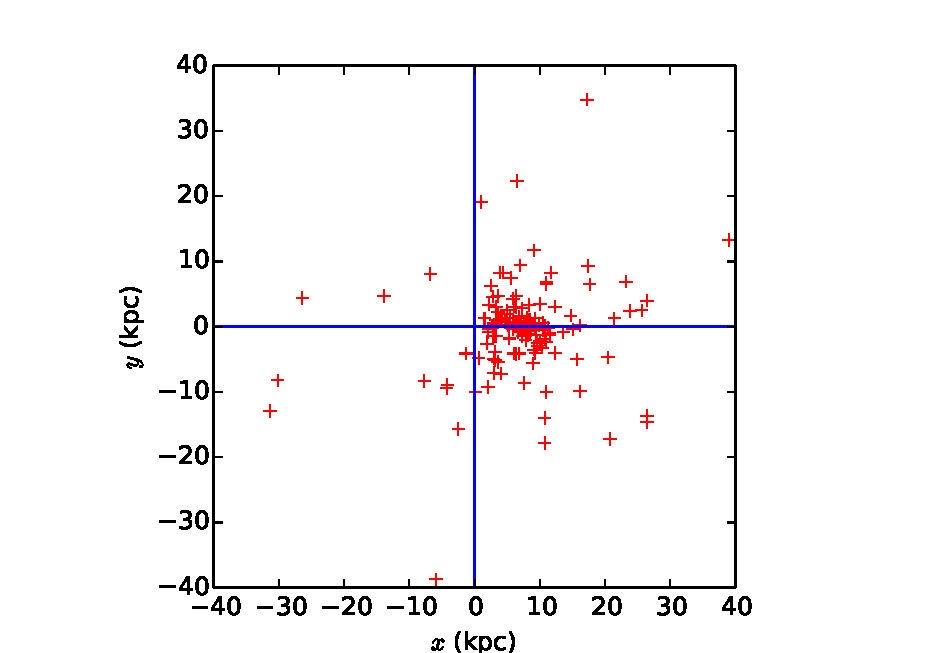
\includegraphics[width=\linewidth]{plan_xOy_GC.pdf}
				\end{minipage}\hfill
				\begin{minipage}{0.33\linewidth}
						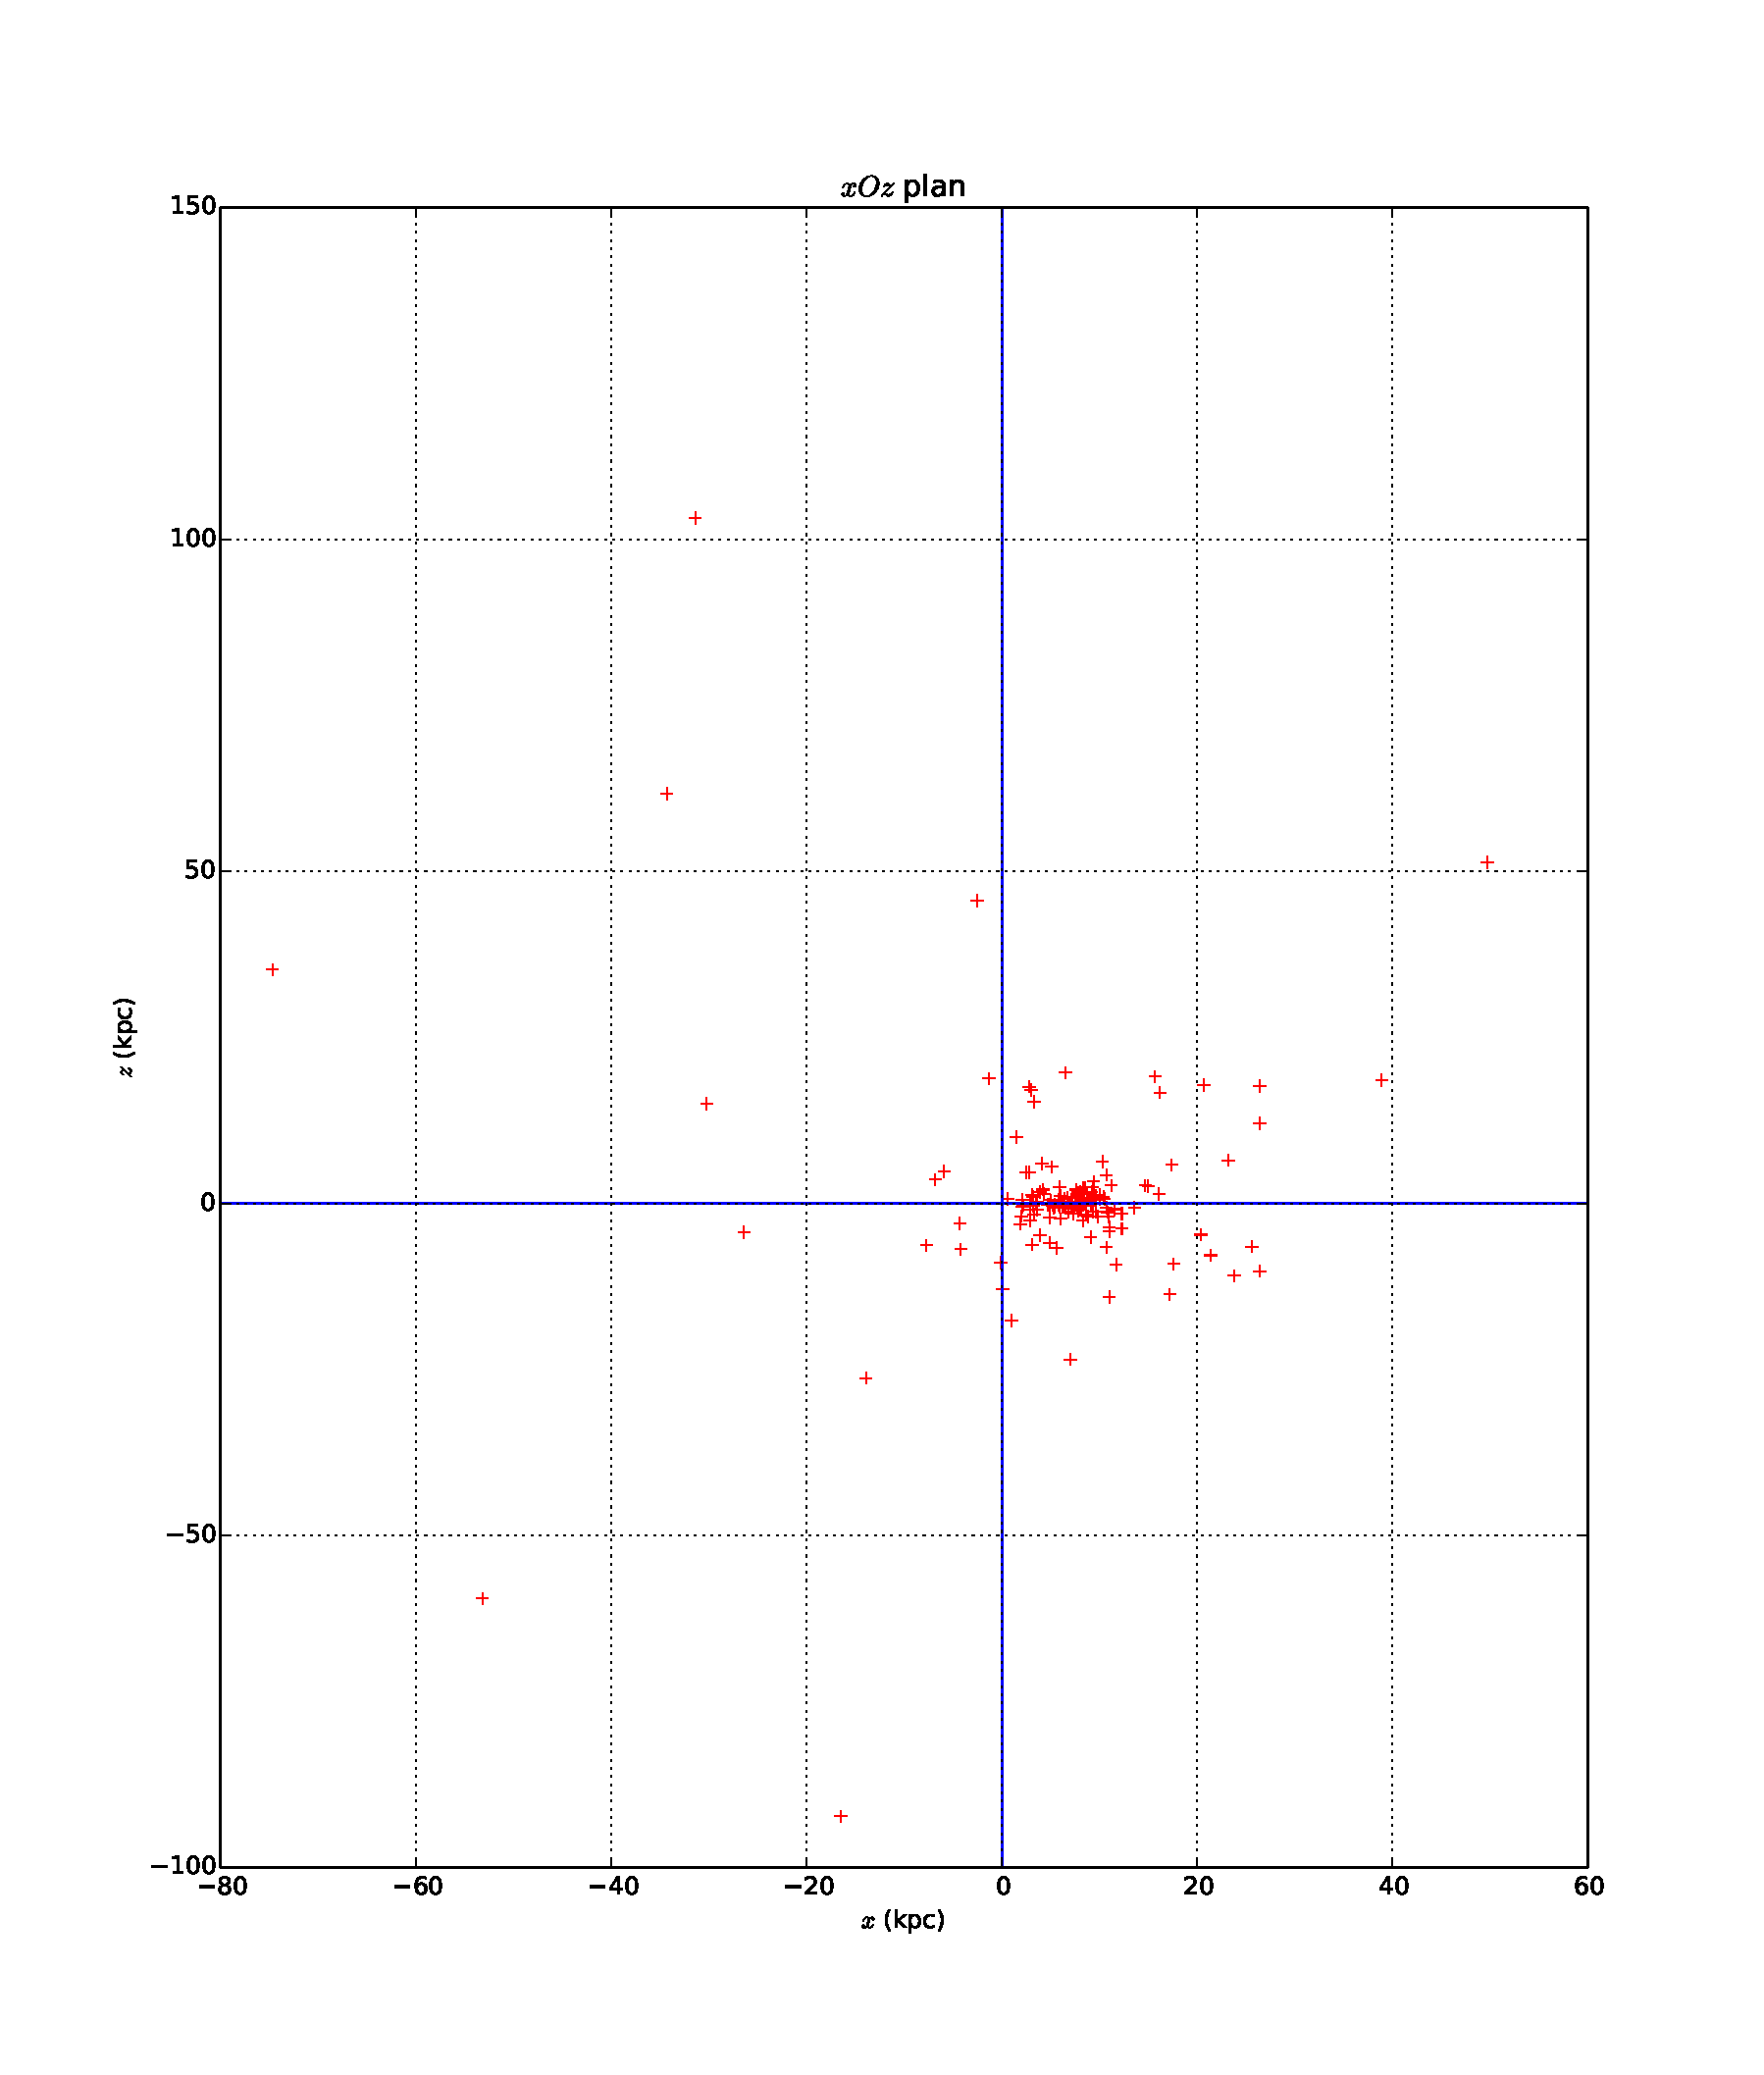
\includegraphics[width=\linewidth]{plan_xOz_GC.pdf}
				\end{minipage}\hfill
				\begin{minipage}{0.33\linewidth}
						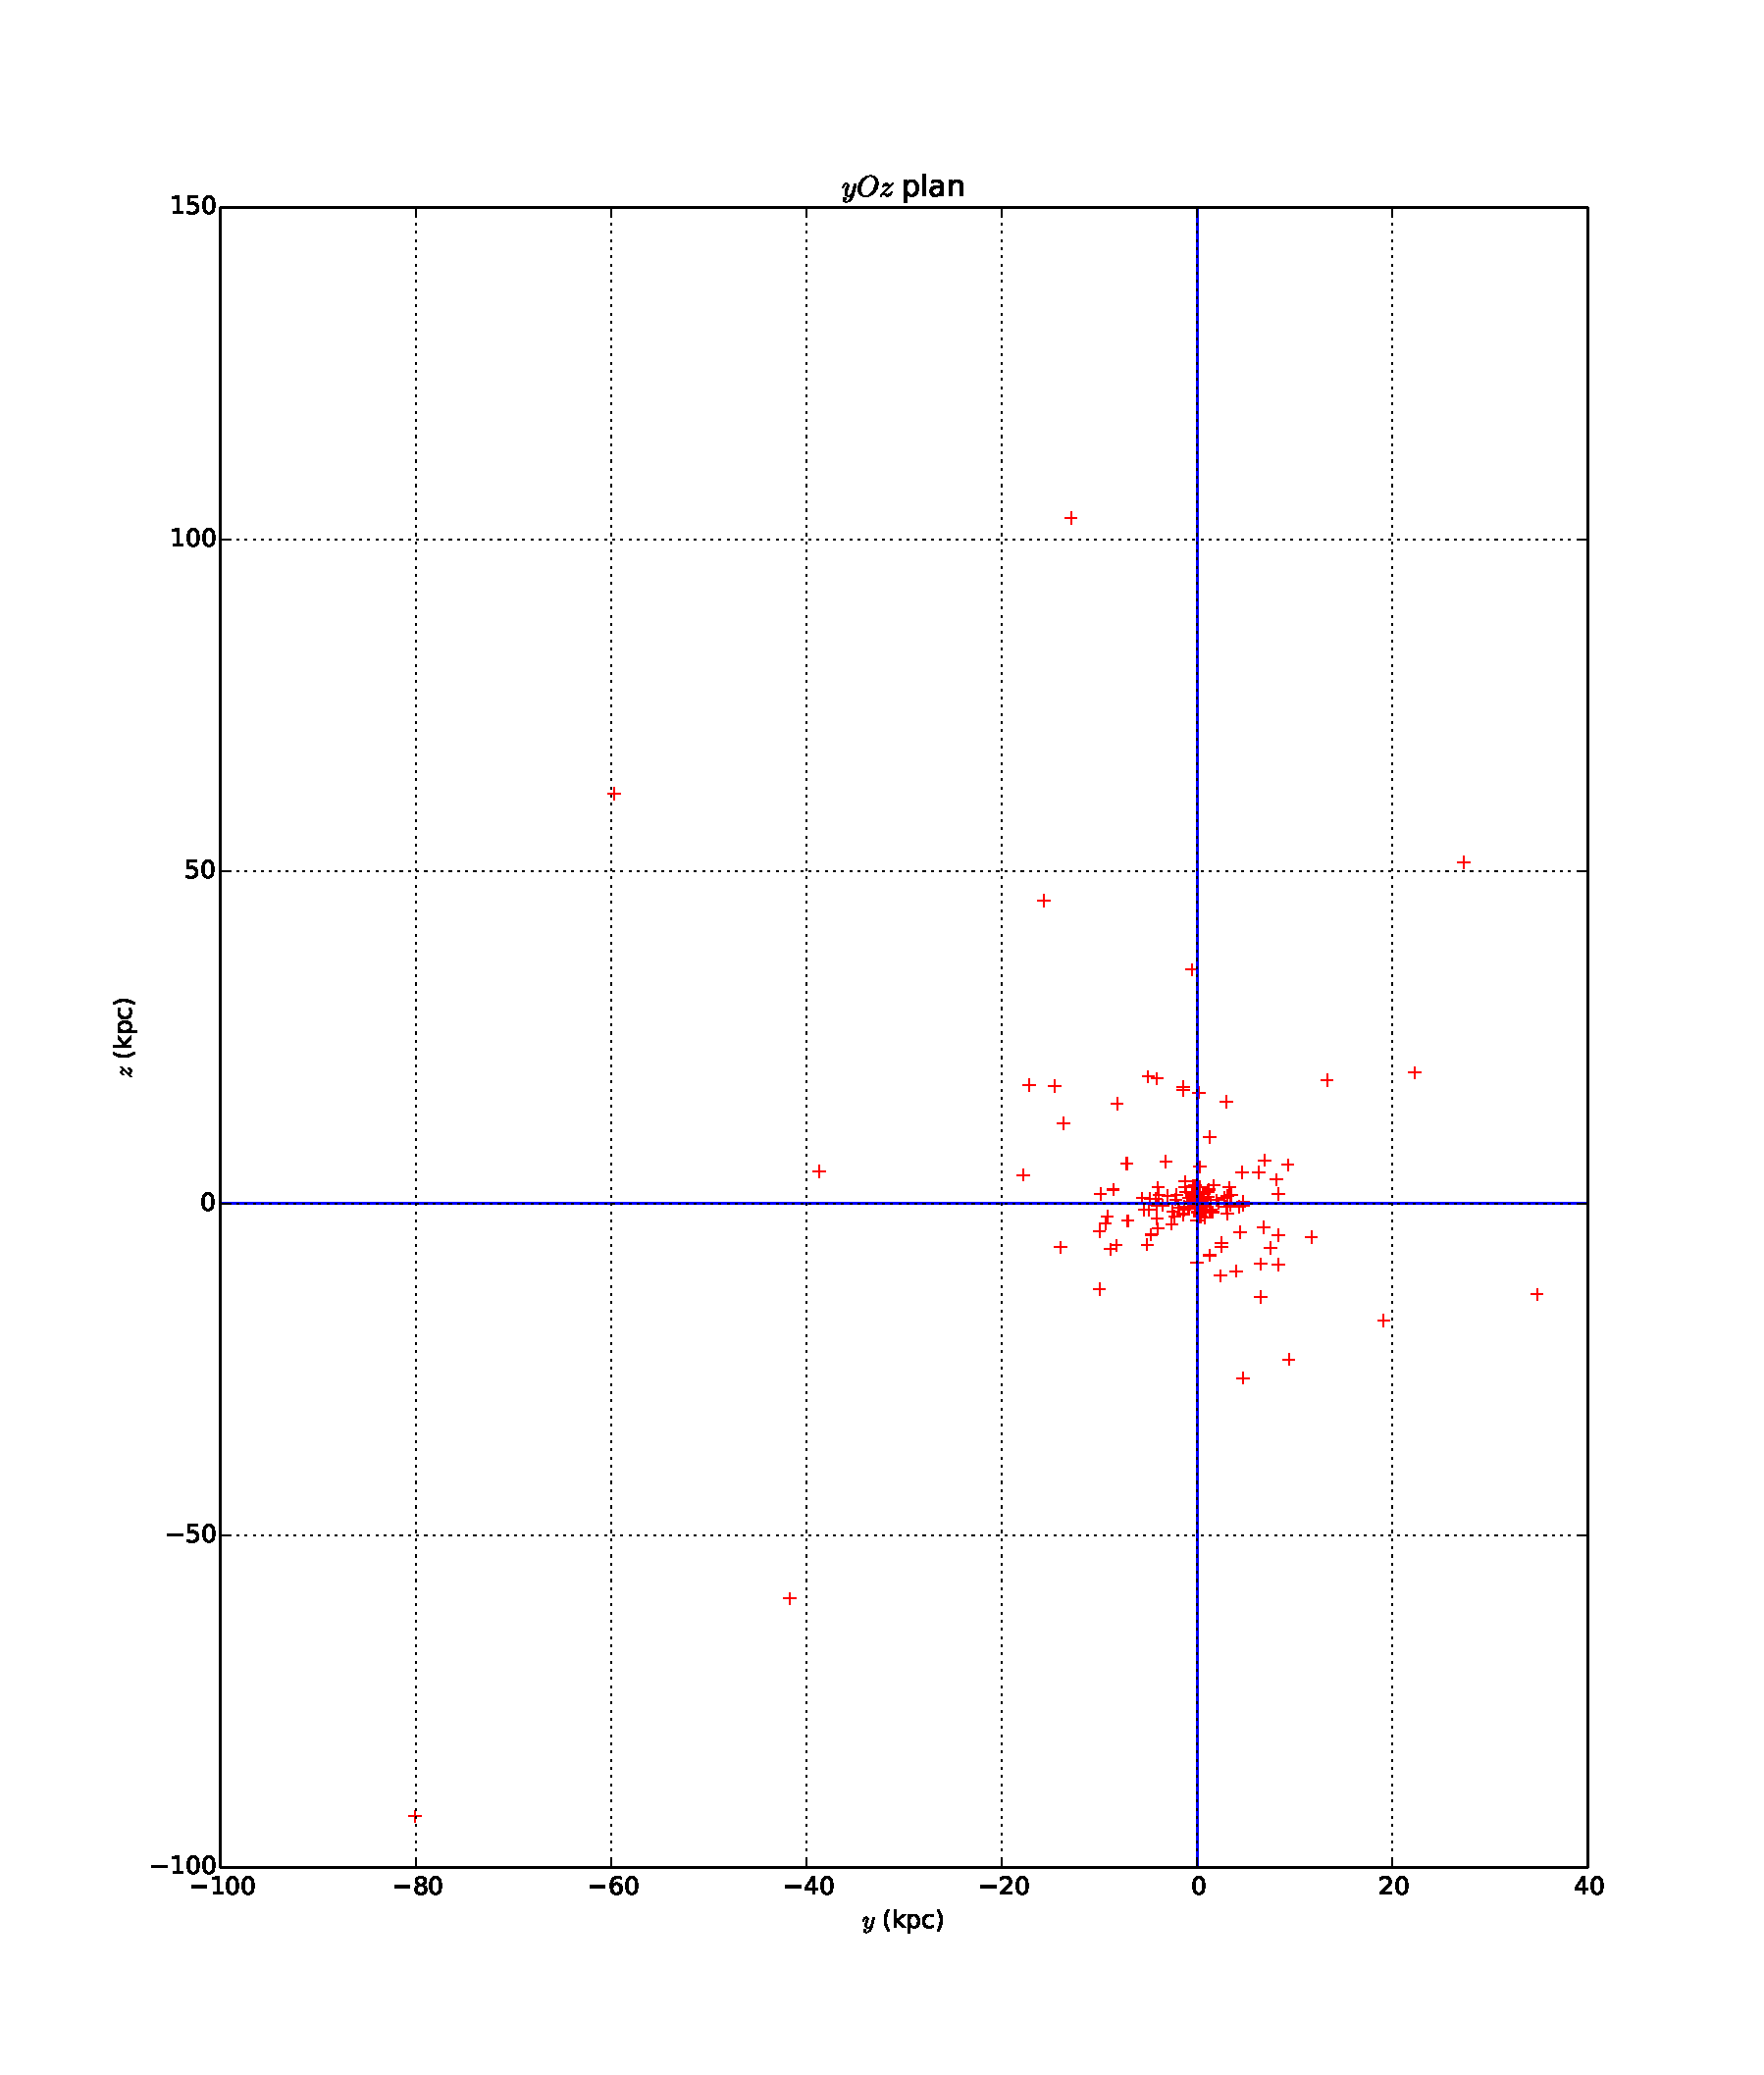
\includegraphics[width=\linewidth]{plan_yOz_GC.pdf}
				\end{minipage}
					\end{center}
				\caption{\label{Fig::Intro::repartition}Répartition des amas globulaires connus dans
				notre galaxie. Les graphiques utilisent le système de coordonnées galactiques (et donc centré sur le soleil).}
			\end{figure}


		\subsection{Profil de densité}

			L'étude des propriétés physiques des amas globulaires s'étale aujourd'hui sur plus d'un siècle d'observations et de
			modélisation. Une caractéristique commune aux amas est leur forme sphérique, l'ellipticité maximale observée étant de l'ordre
			de 10\% et s'explique par une faible rotation solide. Un consensus est maintenant établi sur le fait que leur profil de
			densité volumique de masse -- en abrégé densité et noté $\rho(r)$ -- est un excellent traceur de leur évolution. Les amas
			globulaires se répartissent en deux catégories (voir la figure~\ref{Fig::Intro::images}):
			\begin{itemize}

				\item 80\% des amas présentent une densité caractérisée par 2 régions: le cœur pour lequel la densité est quasiment
					constante ($\rho(r) \approx \mathrm{cte}$) et le halo dans lequel la densité évolue globalement comme une loi
					de puissance ($\rho(r) \propto r^{-\alpha}$): ils ont un profil de type cœur-halo (core-halo dans la
					littérature anglo-saxonne);

				\item la densité du cœur des 20\% restant est remplacée par une loi de puissance. Ils sont dits cœur effondré
					(core-collapsed).

			\end{itemize}

			La plupart des modèles d'amas globulaire sont issus de la sphère isotherme. Nous en
			aborderons certains au cours de ce document. Parmi ces modèles, un en particulier
			permet d'ajuster le profil de densité des amas globulaires durant une grande
			partie de leur évolution: le modèle de King
			(voir~\cite{1966AJ.....71...64K} et le chapitre~\ref{King::Chapitre}).

			\begin{figure}[h]
				\begin{center}
					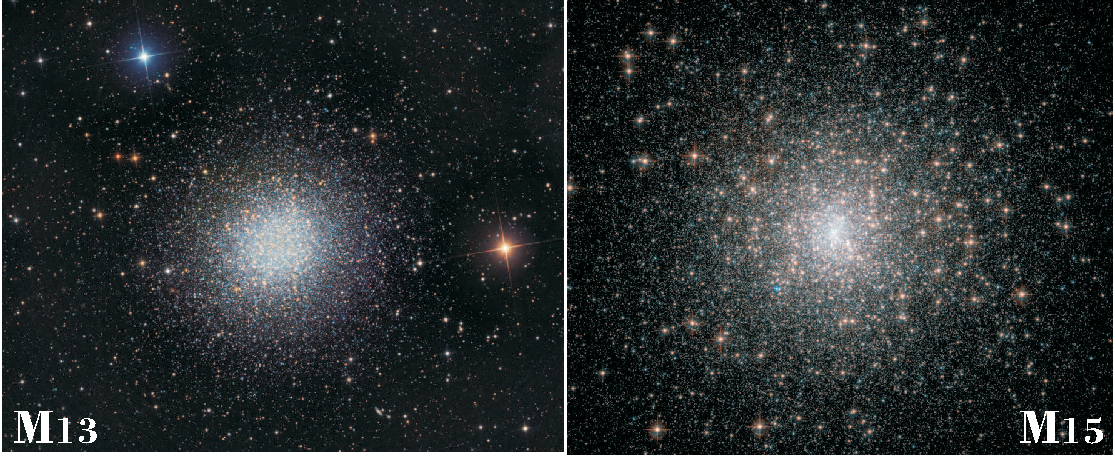
\includegraphics[width=\linewidth]{gc_photo}
				\end{center}
				\begin{minipage}{0.45\textwidth}
					\begin{center}
						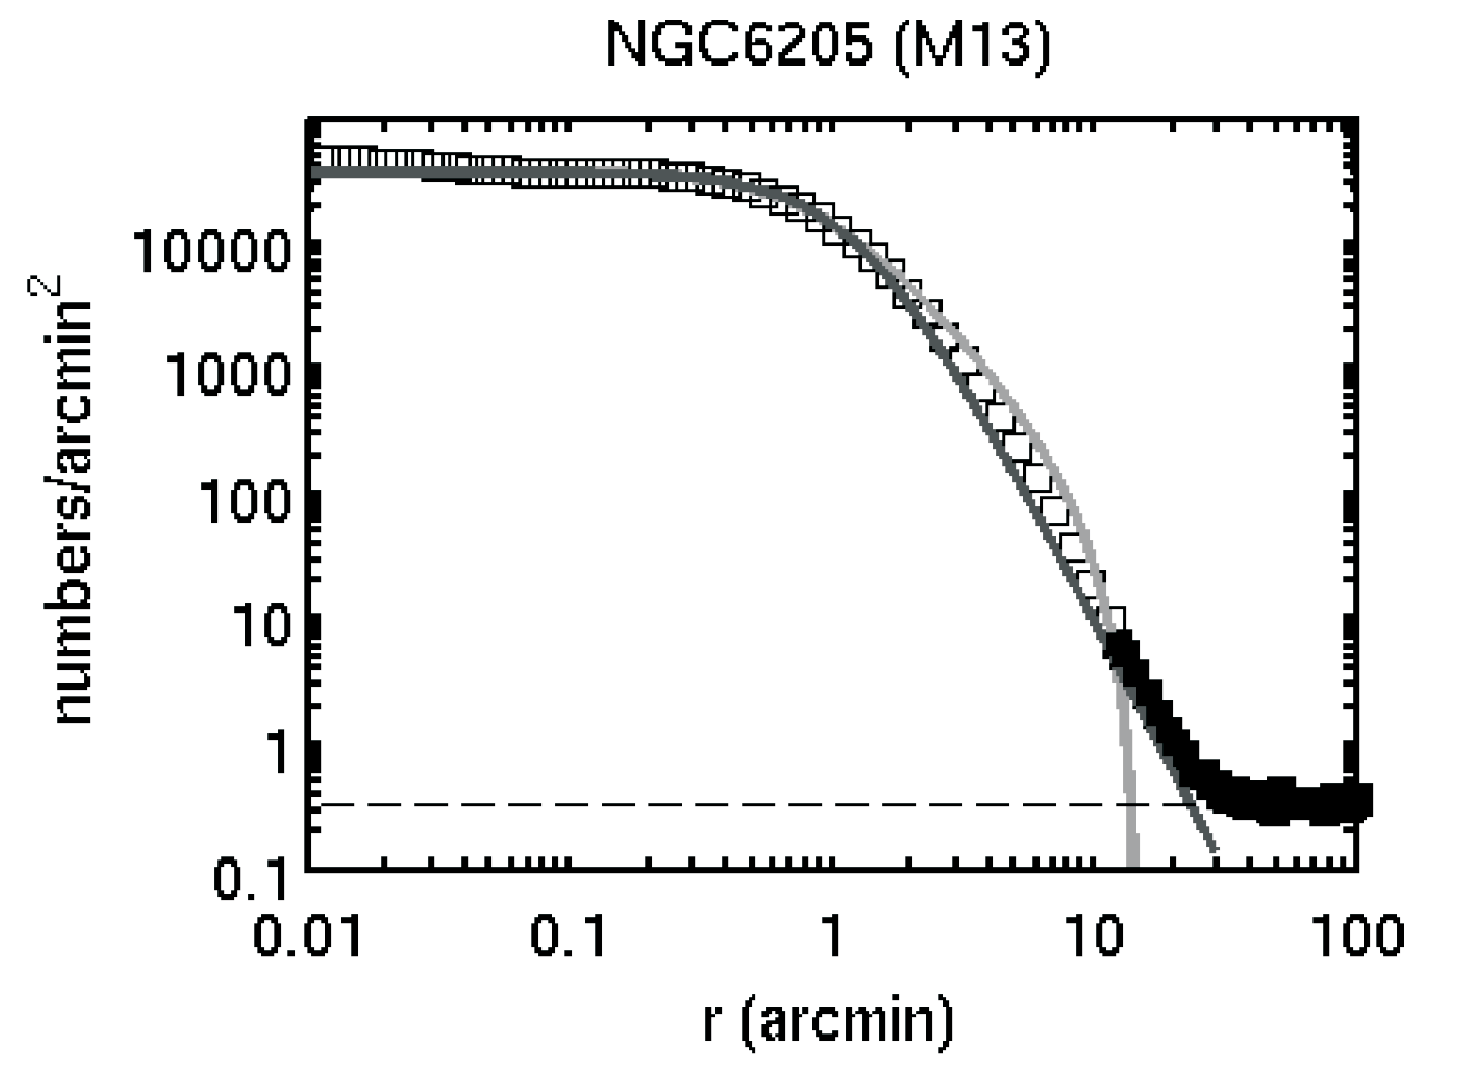
\includegraphics[width=\linewidth]{M13}
					\end{center}
				\end{minipage}\hfill
				\begin{minipage}{0.45\textwidth}
					\begin{center}
						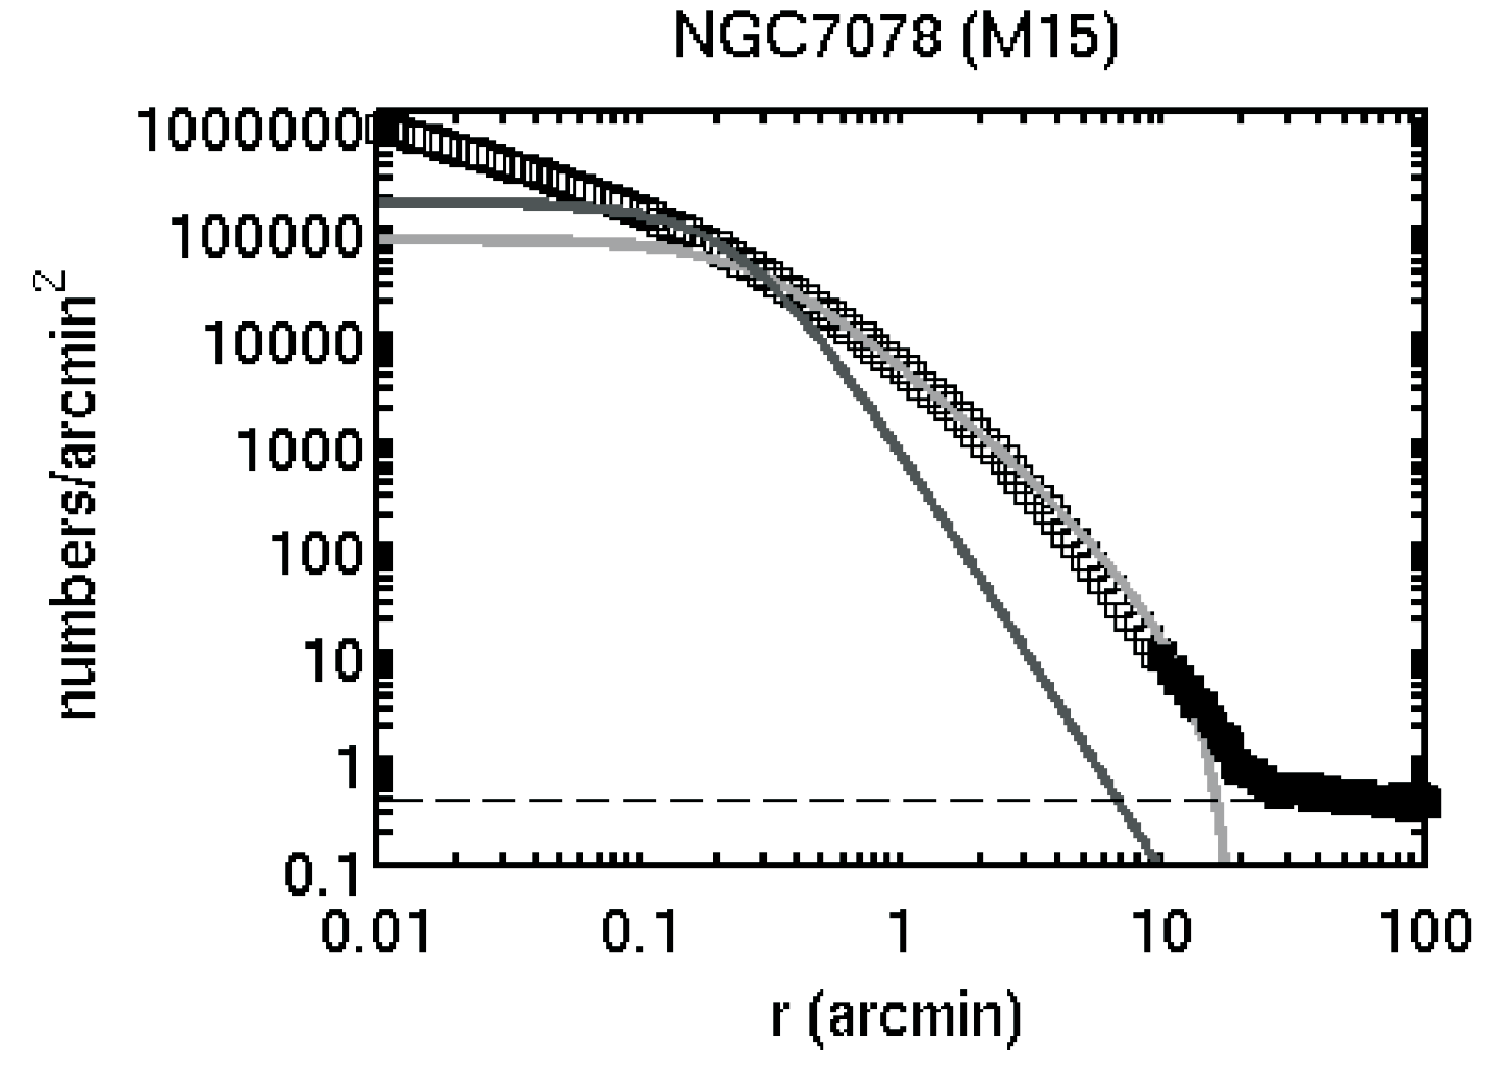
\includegraphics[width=\linewidth]{M15}
					\end{center}
				\end{minipage}
				\caption{\label{Fig::Intro::images}Deux amas globulaires
					caractéristiques et leurs comptages d'étoiles (tiré de~\cite{2010A&A...522A..71J}).
					M13 est un amas présentant une structure cœur-halo,
					M15 est un amas au cœur dit effondré}
			\end{figure}

		\subsection{Simulation numérique des amas globulaires}

			Dès les années 1960, des simulations numériques sont utilisées en plus de la théorie afin de modéliser l'évolution de ces
			objets. Plusieurs méthodes numériques ont été utilisées, les principales sont:
			\begin{itemize}

					\item les simulations Fokker-Planck permettent de
						simuler l'évolution d'un amas sphérique de plusieurs millions
						d'étoiles sur une grande période de temps en quelques
						jours de calcul. Même si ce type de simulation permet d'intégrer une
						certaine forme de dissipation dans l'évolution du système, une telle
						efficacité n'est possible qu'en faisant l'hypothèse que le système
						conserve ses propriétés sphériques et isotropes tout au long de son
						évolution.% L'algorithme utilisé est alors celui de Monte-Carlo;
						Un algorithme de type Monte-Carlo est alors utilisé;

					% \item les simulations Monte-Carlo, elles permettent de
						% simuler l'évolution d'un amas de plusieurs millions
						% d'étoiles sur une grande période de temps en quelques
						% jours, en adaptant les propriétés globales des
						% orbites des étoiles au gré de leur évolution
						% numérique;

					\item les simulations $N$-corps utilisant une méthode de sommation directe modifient à chaque pas de
						temps les positions et vitesses des étoiles du modèle. Ces simulations sont beaucoup plus lentes mais
						laissent plus de liberté au système quant à son évolution.

					% \item les simulations $N$-corps utilisant un tree-code, méthode intermédiaire que nous utiliserons et qui sera
						% détaillée plus loin (voir le chapitre~\ref{Chap::Simu::Analysis}).

			\end{itemize}
			La figure~\ref{Fig::Intro::HeggieFigure}, issue de la présentation de D.~Heggie au trimestre Gravasco, montre les amas du
			catalogue de Harris tracés dans le plan (temps de relaxation)/(magnitude intégrée en bande V). Les droites parallèles
			indiquent le temps que durerait une simulation $N$-Corps (avec une sommation directe) ou Fokker-Planck d'un amas globulaire
			avec ces paramètres. Par exemple, une simulation $N$-Corps de l'évolution dynamique complète de M4 prendrait environ 300 ans
			tandis que son équivalent Fokker-Planck ne prendrait qu'une journée.

			\begin{figure}[h]
				\centering 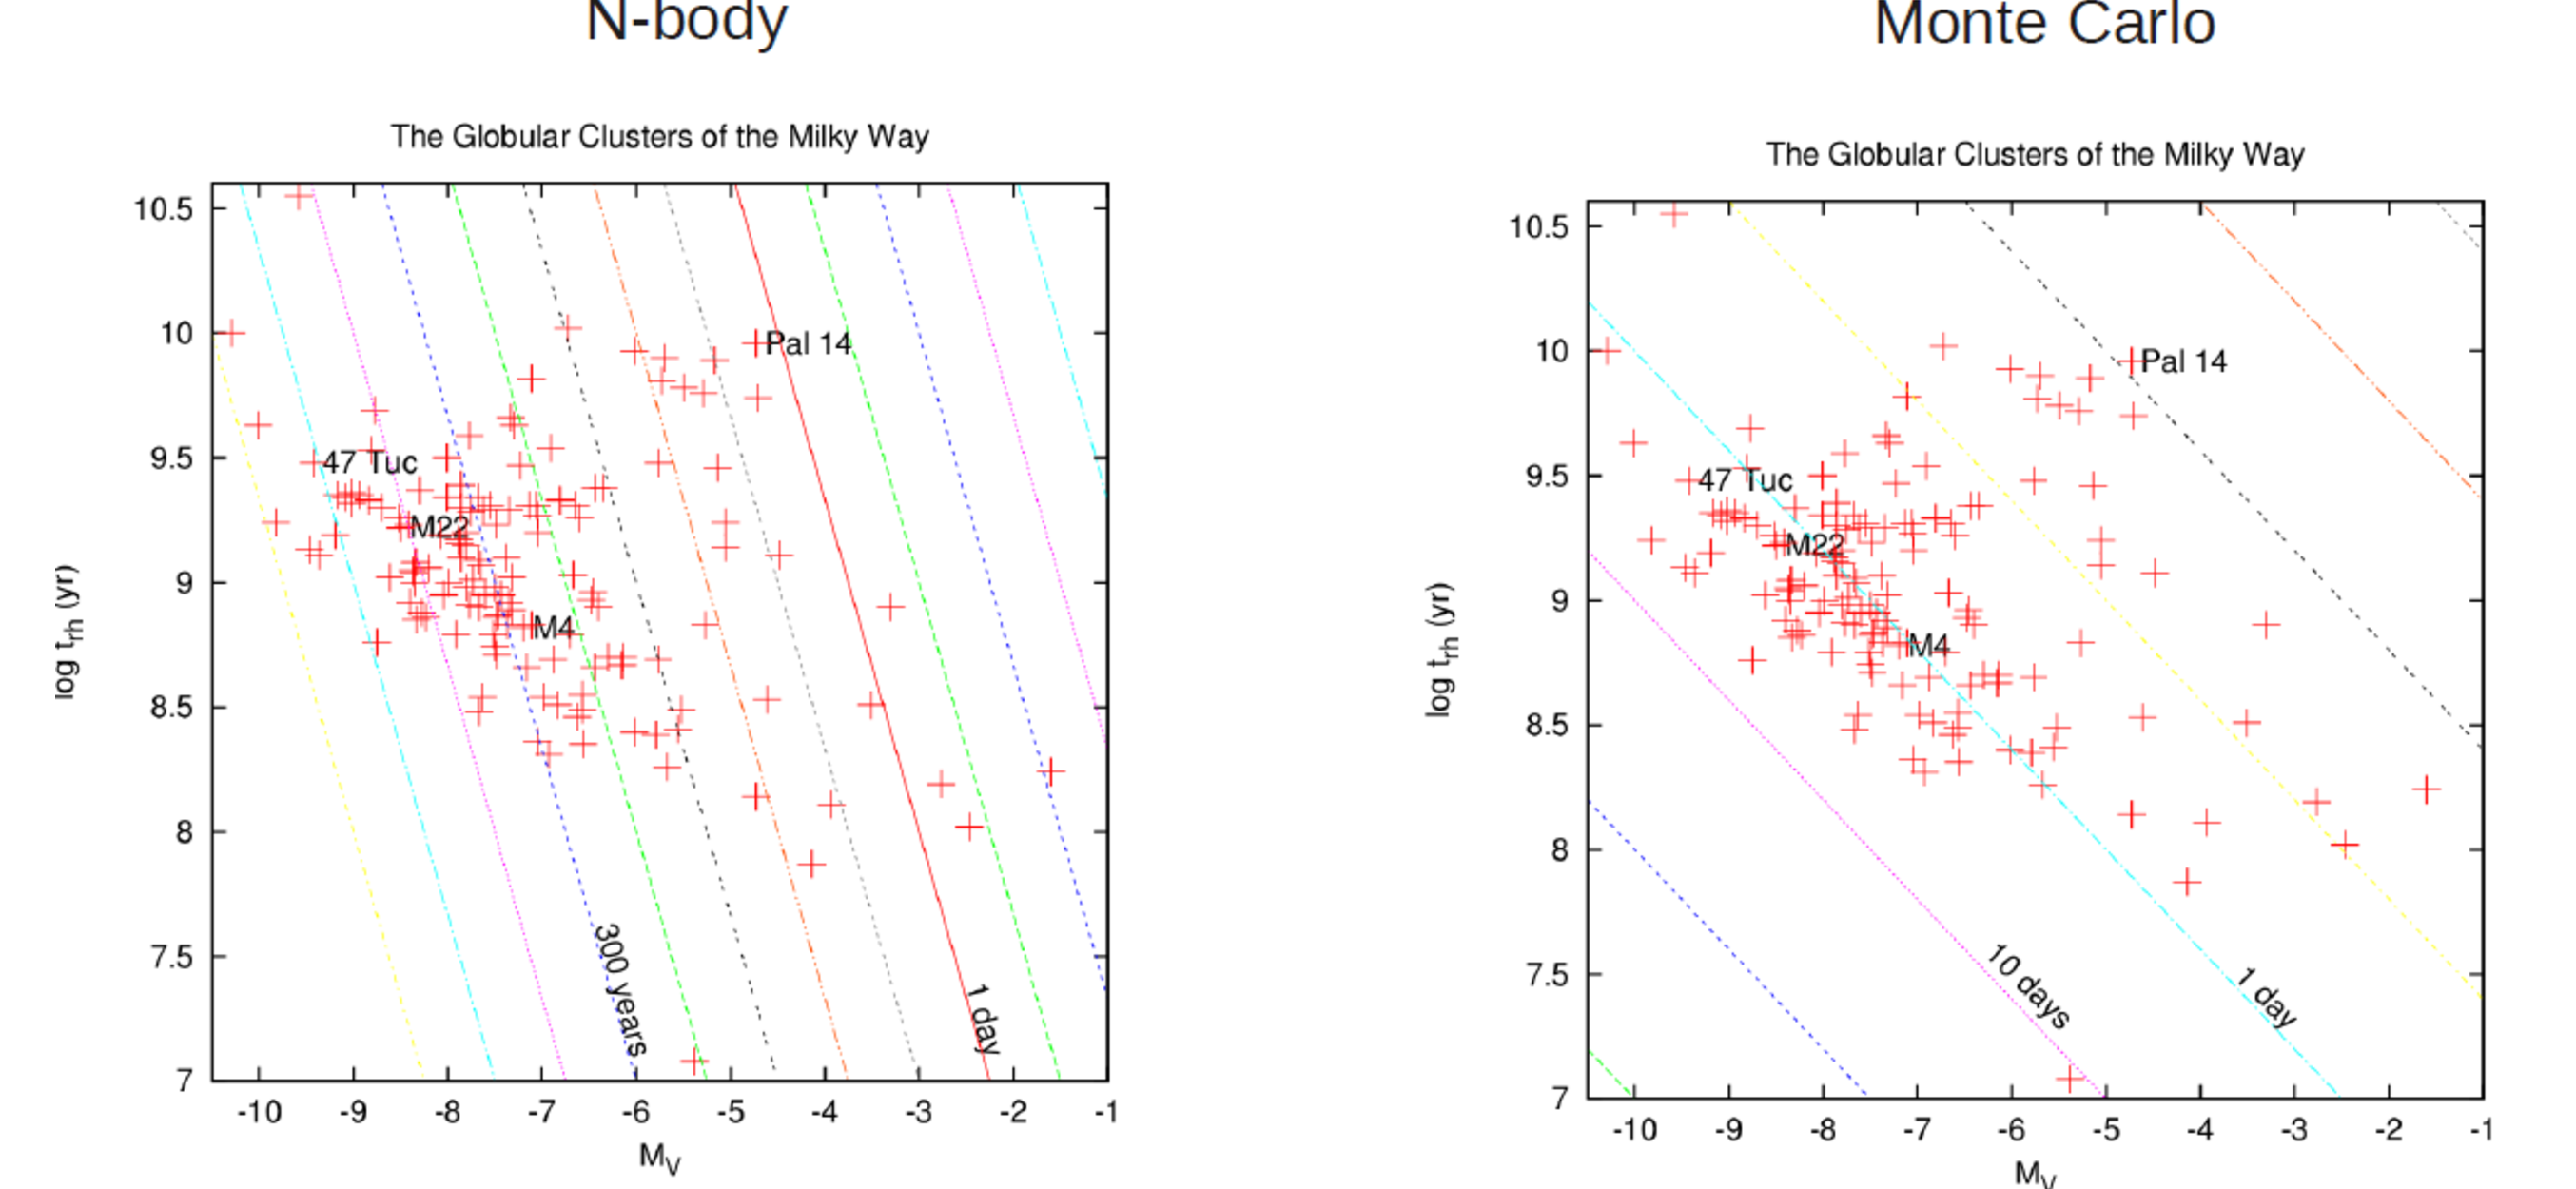
\includegraphics[width=\linewidth]{Heggie_figure.pdf}
				\caption{\label{Fig::Intro::HeggieFigure}Évolution du temps de
				calcul selon l'amas globulaire et du type de simulation.}
			\end{figure}

			Les simulations ont permis de prendre de l'avance sur les observations en
			confirmant certains phénomènes prévus par la théorie, notamment
			les oscillations gravothermales (voir~\cite{1996ApJ...471..796M}). Ce phénomène
			intervient après l'effondrement du cœur, une binaire serrée vient alors
			contrôler la dynamique du centre de l'amas. Sous l'effet d'interactions à 3
			corps, cette binaire est remplacée par une autre produisant un pic de
			densité. Ces pics se succèdent à un rythme dépendant des caractéristiques de
			l'amas.

			% Contrairement aux galaxies
			De façon générique,
			les amas globulaires ne semblent pas contenir
			en leur centre de trou noir massif. Par cet aspect, mais
			aussi par le fait qu'ils ne semblent pas contenir de grandes quantités de
			matière noire, ils se distinguent des galaxies.

		\subsection{Une première étude personnelle}

			Comme nous l'avons précisé plus haut, il est généralement admis que le
			profil de densité est un traceur de l'évolution des amas globulaires. Nous
			n'avons cependant pas trouvé d'étude exhaustive sur ce sujet et avons donc
			tenté de préciser ce lien.
			La principale caractéristique du profil de densité d'un amas globulaire est
			la pente de son halo. Celle-ci n'ayant pas fait l'objet d'une étude globale nous
			avons donc fabriqué notre propre catalogue à partir des données
			de~\cite{Trager-graphe} donnant le profil de brillance de surface en fonction de la taille angulaire
			de chaque amas.


			%Parallèlement, nous avons construit un catalogue
			%des temps de relaxation par collision de ces amas à partir du catalogue de
			%\textsc{Harris}~\cite{Harris}.

			%	Ce qui va nous intéresser ici, c'est de pouvoir lier à chaque étape d'évolution d'un amas, et donc à son âge,
			%	une pente.
				%Notre objectif est de trouver une relation entre l'âge d'un amas et la pente de son halo.
				%Nous avons parlé dans la section précédente du profil de densité
				%comme d'un marqueur de l'évolution des amas globulaires, nous allons
				%voir en quoi.
				%S'il est possible de trouver, à partir de ces profils, plusieurs
				%marqueur d'évolution, celui qui nous intéresse plus particulièrement
				%est la pente du halo. Pour vérifier que cette pente évolue bien avec
				%l'âge dynamique de l'objet, et comment, nous avons utilisé les
				%données du catalogue de \textsc{Harris}~\cite{Harris} qui nous a
				%permis d'obtenir l'âge d'une centaine d'amas
				%globulaire. Pour les profils de densité, nous
				%utilisons~\cite{Trager-graphe}.
				
				%Nous avons donc besoin d'une relation entre cette quantité et l'âge
				%de l'amas, si une telle relation existe.

				% Après avoir déprojeté les profils de brillance de surface
				% pour avoir la densité et donc obtenir la pente du halo, nous
				% l'avons tracé en fonction du temps de relaxation. Nous avons alors
				% ajusté la courbe ainsi obtenue par une droite d'équation $ \alpha =
				% \mathrm{pente} = a \log_{10}(T_c) + b$.

				% La première étape pour transformer les données
				% de~\cite{Trager-graphe} (récupérable ici~\cite{TragerTable}) d'une
				% brillance de surface de l'objet en fonction d'un rayon en seconde
				% d'arc en densité volumique de masse.

				%Le premier traitement à effectuer consiste donc à transformer
				%cette brillance de surface par arc seconde carrée en une densité
				%(~kilogramme par kilomètre au cube~).

				%Une définition de cette brillance de surface, telle qu'elle semble avoir été utilisée, peut-être trouvé dans~\cite{SBP}.
				%Comme indiqué dans ce texte, la brillance de surface va s'écrire :
				%\begin{align}
					%\mu_V = \mu_{\mathrm{ref}} - 2.5 \log_{10}\(\frac{f/\Omega}{f_{\mathrm{ref}}/\Omega_{\mathrm{ref}}}\)
					%\label{mu_V}
				%\end{align}
				%avec $\Omega$ l'angle solide, exprimé en seconde d'arc au carrée, sous lequel nous voyons l'objet.
			%	\begin{align}
			%		\mu_V = m_V - 2.5 \log_{10}\(\frac{(1\mathrm{"})^2}{\Omega}\)
			%		\label{mu-astuce}
			%	\end{align}
			%	avec $m_V$ la magnitude apparente de l'objet sur une seconde d'arc au carrée.

				La brillance de surface utilisée dans cet article est la suivante:
				\begin{align}
					\mu = -2.5 \log\(\frac{10^{-0.4 m_2} - 10^{-0.4 m_1}}{\pi \(r_2^2 - r_1^2\)}\)
					\label{Trager-eq}
				\end{align}
			%	où ils prendraient comme référence les points autour de celui considéré (~ou quelque chose comme ça~),
				$m_i$ étant la magnitude en un point de l'objet et $r_i$ le rayon en seconde d'arc pour ce point.

				La conversion de cette brillance surfacique en densité surfacique de masse est possible
				en connaissant le rapport masse-luminosité de ces amas. L'article~\cite{McL} ne donne cette
				quantité que pour 40 des 150 amas de notre galaxie.
				% Les rapports masse-luminosité dont nous avons besoin pour terminer
				% la conversion peuvent être trouvés dans~\cite{McL},
				% mais cette article ne contient que 40 des 140 amas de notre galaxie.
				Par contre, il est aisé de remarquer que ces rapports sont %en
				répartis dans un intervalle de faible amplitude
				% moyenne très peu différents de la valeur $2$
				avec une
				valeur minimum de $1.87$ pour NGC4147 et une valeur maximum de
				$2.66$ pour NGC6441. Pour simplifier, nous avons utilisé:
				%Dans la suite, nous prendrons donc:
				\begin{align}
					\Upsilon = \dfrac{M}{L} = 2
				\end{align}
				pour les 110 amas dont nous ne connaissons pas $\Upsilon$. %autres amas.
				%Les données de~\cite{Trager-graphe} nous ont donc permis d'obtenir
				Un algorithme de déprojection permet alors d'obtenir la densité $\rho(r)$ de chaque amas du catalogue de Harris.

				%\begin{enumerate}
					%\item $10^{-0.4 m_i}$ est proportionnel à un flux, % (~ou au rapport d'un flux par rapport à un flux de référence !?!~),
					%\item $r_i$ est le rayon de l'objet au point $i$ en seconde d'arc,
					%\item[$\Rightarrow$] nous avons donc bien notre flux par seconde d'arc au carrée.
				%\end{enumerate}
				%Pour pouvoir revenir aux quantités que nous cherchons, il va falloir calculer un peu :
				%\begin{align}
					%\mu = -2.5 \log\(\frac{10^{-0.4 m_2} - 10^{-0.4 m_1}}{\pi \(r_2^2 - r_1^2\)}\) &\equiv -2.5 \log\(\frac{F}{\pi \(r_2^2 - r_1^2\)}\) \text{avec $F$ le flux}\notag \\
					%\intertext{par rapport à toute la documentation que j'ai trouvé, le $\log$ correspond ici à $\log_{10}$ et non à $\ln$.}
					%\Rightarrow \frac{F}{\pi \(r_2^2 - r_1^2\)} &= 10^{-\mu/2.5} \label{F--mu} \\
					%\intertext{Grâce à~\cite{McL}, nous avons les rapports masse luminosité :}
					%\Upsilon &= \frac{M}{L} \label{M/L}\\
					%\intertext{or}
					%F &= \frac{L}{4\pi D^2} \label{def-F}\\
					%\intertext{avec $D$ la distance soleil--amas. D'où}
					%\frac{L}{4 \pi^2 \(r_2^2 - r_1^2\) D^2} &= \frac{M}{4 \pi^2 \Upsilon \(r_2^2 - r_1^2\) D^2} = 10^{-\mu/2.5} \notag \\
					%\intertext{en combinant~\ref{F--mu}, \ref{M/L} et~\ref{def-F}.}
					%\Rightarrow \frac{M}{4\pi \(r_2^2 - r_1^2\)} &= \pi\Upsilon D^2 10^{-\mu/2.5} \notag \\
					%\intertext{Mais $r_2^2 - r_1^2 \propto r_i^2$ doit être converti en mètre :}
					%%r_2^2 - r_1^2 &\propto r_i^2 \Rightarrow \(D \tan(r_i)\)^2 \varpropto \(D r_i\)^2 \notag \\
					%\Rightarrow \frac{M}{4\pi \(D \tan(r_i/3600)\)^2} &= \pi\Upsilon D^2 10^{-\mu/2.5} \label{M-don}
				%\end{align}
				%Normalement, nous avons maintenant une masse surfacique donnée par~\ref{M-don}.
			%	mais, étonnamment, la conversion de seconde d'arc à mètre n'a fait paraître
			%	aucun facteur numérique !!! J'ai peut-être un peu trop truandé.

				%Les rapports masse-luminosité peuvent être trouvés dans~\cite{McL}, mais cette article ne contient que 40 des 140 amas de notre galaxie.
			%	mais il n'y a qu'une quarantaine de rapport comparé à notre échantillon d'environ 140 amas.
				%Par contre, il est aisé de remarquer que ces rapports sont
				%en moyenne très peu différents de la valeur $\Upsilon = 2$ avec une valeur minimum de $1.87$ pour NGC 4147 et une valeur maximum de
				%$2.66$ pour NGC 6441. Dans la suite, nous prendrons donc $\Upsilon = 2$.
			%	Nous avons alors utilisé les données du catalogue pour redimensionner le tout, mais pour passer à la densité, nous avons besoin du rapport masse
			%	sur luminosité de l'amas qui peut-être trouvé dans~\cite{McL}.
			%	Cet article ne donne qu'une quarantaine d'amas sur les 150 de notre galaxie, mais les valeurs de ces rapports étant compris entre $1.87$ pour NGC 4147
			%	(~et quelques autres~) et $2.66$ pour NGC 6441, et tournant surtout autour de $2$, nous pouvons supposer que ces rapports sont les mêmes pour chaque amas et
			%	valent $\Upsilon = \frac{M}{L} = 2$.
			%	Selon~\cite{Trager-graphe}, nous avons donc :
			%	\begin{align}
			%		\mu_V &\propto \text{Flux par $m^{-2}$} = \frac{L}{4\pi D^2} \\
			%		\intertext{or}
			%		L &= \frac{M}{\Upsilon} \notag \\
			%		\intertext{donc}
			%		\mu_V &= \frac{M}{4\pi D^2 \Upsilon} \notag \\
			%		M &= \Upsilon \mu_V 4\pi D^2
			%	\end{align}
			%	avec $D$ la distance entre nous et l'amas. Nous pouvons supposer que cette distance est la même quelque soit l'étoile considéré dans l'amas
			%	(~$D_{min} = 3000\mathrm{pc} \gg R_{amas} \approx 10\mathrm{pc}$~).

			%	Du fait des rapports masse-luminosité manquant, notre échantillon d'une quarantaine d'amas est passé à seulement 12 amas.

				Afin de déterminer la pente du halo, nous
				normalisons cette densité par la densité du cœur, puis mesurons la
				pente dans l'intervalle: %la région vérifiant:
				\begin{align*}
					10^{-4} \leq \dfrac{\rho(r)}{\rho(0)} \leq 0.1.
				\end{align*}
				Nous avons alors construit un catalogue des temps de relaxation par
				collisions et des temps dynamiques de ces amas en utilisant d'une part le catalogue de
				\cite{Harris} et d'autre part en intégrant le profil de densité obtenu
				pour chaque amas.
				Nous obtenons alors les graphiques~\ref{Pente-lin_dim} et~\ref{Pente-Td-lin}. L'ajustement a été effectué à l'aide
				d'une méthode de moindre carré, donnant une valeur de la pente de chaque droite de $-1.31\pm0.44$ pour la
				figure~\ref{Pente-Td-lin} et $-1.23\pm0.46$ pour la figure~\ref{Pente-lin_dim}. La valeur numérique de cette pente
				n'est pas fondamentale, une tendance est cependant bien présente: la pente diminue lorsque le temps dynamique ou le
				temps de collision augmente.

				%Le calcul de pente a été refait en utilisant : les données de
				%l'article~\cite{TragerTable}, le traitement décrit ci-dessus, et en
				%ajustant une droite pour des densités comprises entre $10^{-4}$ et
				%0,1. Nous obtenons alors le graphique~\ref{Pente-lin_dim},
				%l'ajustement utilisant la fonction $f(T_c) = a \log(T_c) + b$ (~les
				%coefficients ont été donnés dans la
				%table~\ref{pente-lin-coeff_dim}~). Nous avons donc maintenant une
				%relation linéaire entre l'âge de l'amas et la pente du halo.

				\begin{figure}[h!]
			%		\centering \includegraphics[scale=0.9]{../Amas/Graphe_Rapport/pente-Tc.pdf}
					\centering 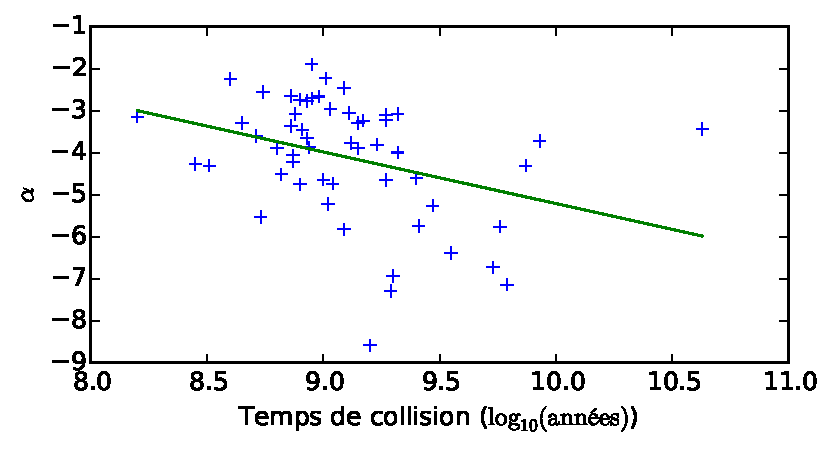
\includegraphics[scale=1.0]{graphe/pente_tc.pdf}
					\caption{Évolution des pentes pour différents âges collisionnels}
					\label{Pente-lin_dim}
				\end{figure}
				%\begin{table}[hbt!]
					%\begin{center}
						%\begin{tabular}{|c|c|}%c|}
							%\hline
							%Coefficient & Valeur \\ %& Erreur \\
							%\hline
							%\hline
							%$a$       &         $-2.3341$   \\ %&    $\pm 0.2075$      (~$32.34\%$~) \\
							%\hline
							%$b$       &         $16.913$   \\  %&    $\pm 1.638$       (~$199.5\%$~) \\
							%\hline
						%\end{tabular}
					%\end{center}
					%\caption{Valeurs des coefficients donnée par l'ajustement pour les pentes pour le temps de croisement}
					%\label{pente-lin-coeff_dim}
				%\end{table}

				%Nous avons également utilisé le catalogue de \textsc{Harris} pour obtenir le lien entre la pente du halo et le temps dynamique
				%grâce à l'équation~\ref{Td:sig}. Nous obtenons alors le graphique~\ref{Pente-Td-lin}.
				\begin{figure}[h!]
			%		\centering \includegraphics[scale=0.9]{../Amas/Graphe_Rapport/pente-Td.pdf}
					\centering 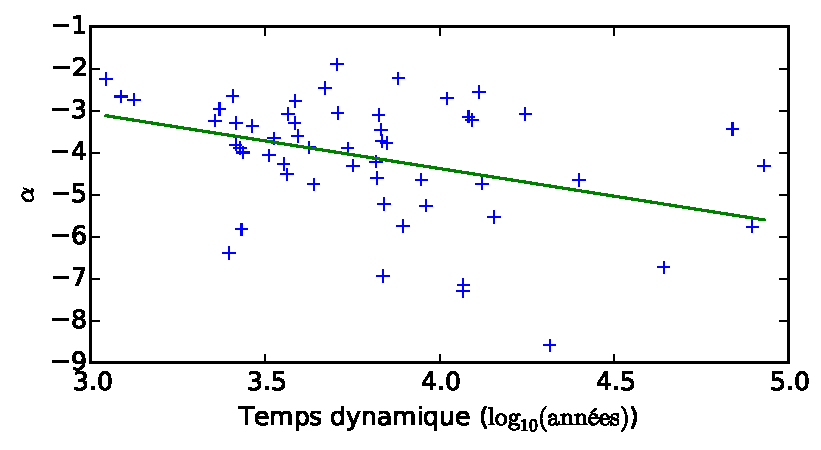
\includegraphics[scale=1.0]{graphe/pente_td.pdf}
					\caption{Évolution des pentes pour différents âges dynamiques}
					\label{Pente-Td-lin}
				\end{figure}
				%\begin{table}[hbt!]
					%\begin{center}
						%\begin{tabular}{|c|c|}%c|}
							%\hline
							%Coefficient & Valeur \\ %& Erreur \\
							%\hline
							%\hline
							%$a$       &        $-1.6567$   \\ %&   $\pm 0.6523$      (~$278.9\%$~) \\
							%\hline
							%$b$       &        $1.8927$     \\ %&   $\pm 2.825$       (~$88.57\%$~) \\
							%\hline
						%\end{tabular}
					%\end{center}
					%\caption{Valeurs des coefficients donnée par l'ajustement pour les pentes pour le temps dynamique}
					%\label{pente-Td-lin-coeff}
				%\end{table}

				%Sur la figure~\ref{Pente-lin_dim}, nous pouvons noter la présence de 2 points avec des pentes inférieures à $-10$. Ces points correspondent aux amas NGC 5024 et NGC 5139
				%(~leurs densités sont donnée en annexe, page~\pageref{Graphe-bofbof}~) pour lesquelles la détermination des pentes n'a pas été très concluante.
				%\FloatBarrier

		%\subsection{Préliminaire}
%	Ce qui va nous intéresser ici, c'est de pouvoir lier à chaque étape d'évolution d'un amas, et donc à son âge,
%	une pente.
	Notre objectif est de trouver une relation entre l'âge d'un amas et la pente de son halo.
	%Nous avons donc besoin d'une relation entre cette quantité et l'âge de l'amas, si une telle relation existe.
	Nous avons alors utilisé le temps de relaxation donné dans le catalogue de \textsc{Harris}~\cite{Harris}.
	Pour obtenir les pentes des amas, nous avons utilisé les relevés observationnels~\cite{Trager-graphe}. % (~les données ainsi obtenues et utilisées sont dans la table~\ref{pente-Tc:BSP}~).
	Nous avons commencé par calculer les pentes directement sur les courbes avec un double décimètre, n'ayant alors pas pu obtenir les données correspondant aux graphiques.
	Après avoir tracé la pente mesurée en fonction du temps de relaxation à 2 corps, nous avons ajusté la
	courbe ainsi obtenue par une droite d'équation $ \alpha = \mathrm{pente} = a \log_{10}(T_c) + b$ (~graphe~\ref{Pente-lin}~).
	\begin{figure}[hbt!]
		\centering \includegraphics[scale=0.9]{graphe/Pente-Tc.pdf}
		\caption{Évolution des pentes pour différents âges}
		\label{Pente-lin}
	\end{figure}
%	\begin{table}[hbt!]
%		\begin{center}
%			\begin{tabular}{|c|c|c|}
%				\hline
%				Coefficient & Valeur & Erreur \\
%				\hline
%				\hline
%				$a$       &        $-1.19506$   &   $\pm 0.1576$ (~$13.19\%$~) \\
%				\hline
%				$b$       &        $2.52082$     &   $\pm 1.213$   (~$48.11\%$~) \\
%				\hline
%			\end{tabular}
%		\end{center}
%		\caption{Valeur des coefficients donnée par l'ajustement pour les pentes}
%		\label{pente-lin-coeff}
%	\end{table}

	Cette approche indiquant clairement une relation linéaire entre ces deux paramètres, nous avons décidé d'entreprendre une démarche plus globale et automatique.
	Pour commencer, nous avons donc récupéré les données auprès des auteurs de l'article sur~\cite{TragerTable}. Nous nous sommes alors confronté au problème des unités.

\subsection{Retraitement}
	Le graphique~\ref{Pente-lin} a été obtenu en utilisant~\cite{Trager-graphe} avec ses unités. % (~les données permettant de retracer, nous les avons finalement trouvé,
%	les graphiques de cet article sont données dans~\cite{TragerTable}~).
	La pente donnée ici n'est donc pas la pente de la densité, mais de la brillance de surface de l'objet en fonction d'un rayon en seconde d'arc.
	Le premier traitement à effectuer consiste donc à transformer cette brillance de surface par arc seconde carrée en une densité (~kilogramme par kilomètre au cube~).

	Une définition de cette brillance de surface, telle qu'elle semble avoir été utilisée, peut-être trouvé dans~\cite{SBP}.
	Comme indiqué dans ce texte, la brillance de surface va s'écrire :
	\begin{align}
		\mu_V = \mu_{\mathrm{ref}} - 2.5 \log_{10}\(\frac{f/\Omega}{f_{\mathrm{ref}}/\Omega_{\mathrm{ref}}}\)
		\label{mu_V}
	\end{align}
	avec $\Omega$ l'angle solide, exprimé en seconde d'arc au carrée, sous lequel nous voyons l'objet.
%	\begin{align}
%		\mu_V = m_V - 2.5 \log_{10}\(\frac{(1\mathrm{"})^2}{\Omega}\)
%		\label{mu-astuce}
%	\end{align}
%	avec $m_V$ la magnitude apparente de l'objet sur une seconde d'arc au carrée.

	Cette définition rappelle celle de~\cite{Trager-graphe}, section~3.2.3 :
	\begin{align}
		\mu = -2.5 \log\(\frac{10^{-0.4 m_2} - 10^{-0.4 m_1}}{\pi \(r_2^2 - r_1^2\)}\)
		\label{Trager-eq}
	\end{align}
%	où ils prendraient comme référence les points autour de celui considéré (~ou quelque chose comme ça~),
	$m_i$ étant la magnitude en un point de l'objet et $r_i$ le rayon en seconde d'arc pour ce point.
	Par conséquent, les unités de $\mu$ sont un flux par arc seconde carrée en échelle logarithmique :
	\begin{enumerate}
		\item $10^{-0.4 m_i}$ est proportionnel à un flux, % (~ou au rapport d'un flux par rapport à un flux de référence !?!~),
		\item $r_i$ est le rayon de l'objet au point $i$ en seconde d'arc,
		\item[$\Rightarrow$] nous avons donc bien notre flux par seconde d'arc au carrée.
	\end{enumerate}
	Pour pouvoir revenir aux quantités que nous cherchons, il va falloir calculer un peu :
	\begin{align}
		\mu = -2.5 \log\(\frac{10^{-0.4 m_2} - 10^{-0.4 m_1}}{\pi \(r_2^2 - r_1^2\)}\) &\equiv -2.5 \log\(\frac{F}{\pi \(r_2^2 - r_1^2\)}\) \text{avec $F$ le flux}\notag \\
		\intertext{par rapport à toute la documentation que j'ai trouvé, le $\log$ correspond ici à $\log_{10}$ et non à $\ln$.}
		\Rightarrow \frac{F}{\pi \(r_2^2 - r_1^2\)} &= 10^{-\mu/2.5} \label{F--mu} \\
		\intertext{Grâce à~\cite{McL}, nous avons les rapports masse luminosité :}
		\Upsilon &= \frac{M}{L} \label{M/L}\\
		\intertext{or}
		F &= \frac{L}{4\pi D^2} \label{def-F}\\
		\intertext{avec $D$ la distance soleil--amas. D'où}
		\frac{L}{4 \pi^2 \(r_2^2 - r_1^2\) D^2} &= \frac{M}{4 \pi^2 \Upsilon \(r_2^2 - r_1^2\) D^2} = 10^{-\mu/2.5} \notag \\
		\intertext{en combinant~\ref{F--mu}, \ref{M/L} et~\ref{def-F}.}
		\Rightarrow \frac{M}{4\pi \(r_2^2 - r_1^2\)} &= \pi\Upsilon D^2 10^{-\mu/2.5} \notag \\
		\intertext{Mais $r_2^2 - r_1^2 \propto r_i^2$ doit être converti en mètre :}
		%r_2^2 - r_1^2 &\propto r_i^2 \Rightarrow \(D \tan(r_i)\)^2 \varpropto \(D r_i\)^2 \notag \\
		\Rightarrow \frac{M}{4\pi \(D \tan(r_i/3600)\)^2} &= \pi\Upsilon D^2 10^{-\mu/2.5} \label{M-don}
	\end{align}
	Normalement, nous avons maintenant une masse surfacique donnée par~\ref{M-don}.
%	mais, étonnamment, la conversion de seconde d'arc à mètre n'a fait paraître
%	aucun facteur numérique !!! J'ai peut-être un peu trop truandé.

	Les rapports masse-luminosité peuvent être trouvés dans~\cite{McL}, mais cette article ne contient que 40 des 140 amas de notre galaxie.
%	mais il n'y a qu'une quarantaine de rapport comparé à notre échantillon d'environ 140 amas.
	Par contre, il est aisé de remarquer que ces rapports sont
	en moyenne très peu différents de la valeur $\Upsilon = 2$ avec une valeur minimum de $1.87$ pour NGC 4147 et une valeur maximum de
	$2.66$ pour NGC 6441. Dans la suite, nous prendrons donc $\Upsilon = 2$.
%	Nous avons alors utilisé les données du catalogue pour redimensionner le tout, mais pour passer à la densité, nous avons besoin du rapport masse
%	sur luminosité de l'amas qui peut-être trouvé dans~\cite{McL}.
%	Cet article ne donne qu'une quarantaine d'amas sur les 150 de notre galaxie, mais les valeurs de ces rapports étant compris entre $1.87$ pour NGC 4147
%	(~et quelques autres~) et $2.66$ pour NGC 6441, et tournant surtout autour de $2$, nous pouvons supposer que ces rapports sont les mêmes pour chaque amas et
%	valent $\Upsilon = \frac{M}{L} = 2$.
%	Selon~\cite{Trager-graphe}, nous avons donc :
%	\begin{align}
%		\mu_V &\propto \text{Flux par $m^{-2}$} = \frac{L}{4\pi D^2} \\
%		\intertext{or}
%		L &= \frac{M}{\Upsilon} \notag \\
%		\intertext{donc}
%		\mu_V &= \frac{M}{4\pi D^2 \Upsilon} \notag \\
%		M &= \Upsilon \mu_V 4\pi D^2
%	\end{align}
%	avec $D$ la distance entre nous et l'amas. Nous pouvons supposer que cette distance est la même quelque soit l'étoile considéré dans l'amas
%	(~$D_{min} = 3000\mathrm{pc} \gg R_{amas} \approx 10\mathrm{pc}$~).

%	Du fait des rapports masse-luminosité manquant, notre échantillon d'une quarantaine d'amas est passé à seulement 12 amas.

\subsection{Résultat}
	Le calcul de pente a été refait en utilisant : les données de l'article~\cite{TragerTable}, le traitement décrit ci-dessus, et le critère donné dans la section~\ref{pente-critére}.
	Nous obtenons alors le graphique~\ref{Pente-lin_dim}, l'ajustement utilisant la fonction
	$f(T_c) = a \log(T_c) + b$ (~les coefficients ont été donnés dans la table~\ref{pente-lin-coeff_dim}~).
	Nous avons donc maintenant une relation linéaire entre l'âge de l'amas et la pente du halo.

	\begin{figure}[hbt!]
%		\centering \includegraphics[scale=0.9]{../Amas/Graphe_Rapport/pente-Tc.pdf}
		\centering \includegraphics[scale=0.9]{graphe/pente-Tc.pdf}
		\caption{Évolution des pentes pour différents âges}
		\label{Pente-lin_dim}
	\end{figure}
	\begin{table}[hbt!]
		\begin{center}
			\begin{tabular}{|c|c|}%c|}
				\hline
				Coefficient & Valeur \\ %& Erreur \\
				\hline
				\hline
				$a$       &         $-2.3341$   \\ %&    $\pm 0.2075$      (~$32.34\%$~) \\
				\hline
				$b$       &         $16.913$   \\  %&    $\pm 1.638$       (~$199.5\%$~) \\
				\hline
			\end{tabular}
		\end{center}
		\caption{Valeurs des coefficients donnée par l'ajustement pour les pentes pour le temps de croisement}
		\label{pente-lin-coeff_dim}
	\end{table}

	Nous avons également utilisé le catalogue de \textsc{Harris} pour obtenir le lien entre la pente du halo et le temps dynamique
	grâce à l'équation~\ref{Td:sig}. Nous obtenons alors le graphique~\ref{Pente-Td-lin}.
	\begin{figure}[hbt!]
%		\centering \includegraphics[scale=0.9]{../Amas/Graphe_Rapport/pente-Td.pdf}
		\centering \includegraphics[scale=0.9]{graphe/pente-Td.pdf}
		\caption{Évolution des pentes pour différents âges dynamiques}
		\label{Pente-Td-lin}
	\end{figure}
	\begin{table}[hbt!]
		\begin{center}
			\begin{tabular}{|c|c|}%c|}
				\hline
				Coefficient & Valeur \\ %& Erreur \\
				\hline
				\hline
				$a$       &        $-1.6567$   \\ %&   $\pm 0.6523$      (~$278.9\%$~) \\
				\hline
				$b$       &        $1.8927$     \\ %&   $\pm 2.825$       (~$88.57\%$~) \\
				\hline
			\end{tabular}
		\end{center}
		\caption{Valeurs des coefficients donnée par l'ajustement pour les pentes pour le temps dynamique}
		\label{pente-Td-lin-coeff}
	\end{table}

	Sur la figure~\ref{Pente-lin_dim}, nous pouvons noter la présence de 2 points avec des pentes inférieures à $-10$. Ces points correspondent aux amas NGC 5024 et NGC 5139
	(~leurs densités sont donnée en annexe, page~\pageref{Graphe-bofbof}~) pour lesquelles la détermination des pentes n'a pas été très concluante.
	\FloatBarrier



	%\section{Interprétation}

%Nous avons maintenant une équation liant la valeur de la pente au temps de relaxation : $ \mathrm{pente} = \alpha = d * \log_{10}(T_c) + e $ (~coefficients table~\ref{pente-lin-coeff_dim}~)
%et une autre liant la pente à $W_0$ : $ \alpha = a e^{ b W_0 } + c $.
%En combinant ces deux équations, nous pouvons obtenir une relation entre le temps de
%relaxation et $W_0$ :
%\begin{align}
	%\mathrm{pente} &= d \log_{10}(T_c) + e = a e^{b W_0} + c \notag \\
	%\Rightarrow W_0 &= \frac{1}{b} \ln\( \frac{d \log_{10}(T_c) + e - c}{a} \) \label{Tc:W0->fct}
%\end{align}
%avec :
%\begin{table}[h!]
	%\begin{center}
		%\begin{tabular}{|c|r|}
			%\hline
			%Coefficient	&	Valeur \\
			%\hline
			%\hline
			%$a$		&	$ -10.0698 $ \\
				%\hline
			%$b$		&	$ 0.220152 $ \\
			%\hline
			%$c$		&	$ -1.53409 $ \\
			%\hline
			%$d$		&	$ -2.3341 $ \\
			%\hline
			%$e$		&	$ 16.913 $ \\
			%\hline
		%\end{tabular}
	%\end{center}
%\end{table}

%Le comportement que nous avions observé en étudiant le modèle de \textsc{King}, à savoir une évolution de la pente avec $W_0$, se retrouve avec l'âge de notre amas. Ce qui nous a permis de relier
%l'âge et $W_0$.
%Il nous reste à interpreter ces résultats, ce que nous allons faire dans la section suivante.
		%Nous avons maintenant une équation liant la valeur de la pente au temps de relaxation : $ \mathrm{pente} = \alpha = d * \log_{10}(T_c) + e $ (~coefficients table~\ref{pente-lin-coeff_dim}~)
et une autre liant la pente à $W_0$ : $ \alpha = a e^{ b W_0 } + c $.
En combinant ces deux équations, nous pouvons obtenir une relation entre le temps de
relaxation et $W_0$ :
\begin{align}
	\mathrm{pente} &= d \log_{10}(T_c) + e = a e^{b W_0} + c \notag \\
	\Rightarrow W_0 &= \frac{1}{b} \ln\( \frac{d \log_{10}(T_c) + e - c}{a} \) \label{Tc:W0->fct}
\end{align}
avec :
\begin{table}[h!]
	\begin{center}
		\begin{tabular}{|c|r|}
			\hline
			Coefficient	&	Valeur \\
			\hline
			\hline
			$a$		&	$ -10.0698 $ \\
				\hline
			$b$		&	$ 0.220152 $ \\
			\hline
			$c$		&	$ -1.53409 $ \\
			\hline
			$d$		&	$ -2.3341 $ \\
			\hline
			$e$		&	$ 16.913 $ \\
			\hline
		\end{tabular}
	\end{center}
\end{table}

Le comportement que nous avions observé en étudiant le modèle de \textsc{King}, à savoir une évolution de la pente avec $W_0$, se retrouve avec l'âge de notre amas. Ce qui nous a permis de relier
l'âge et $W_0$.
Il nous reste à interpreter ces résultats, ce que nous allons faire dans la section suivante.


	%\section{Petit Scénario\label{petit_scenar}}

%Nous avons vu que les courbes~\ref{King_Modele-test} peuvent être divisées en deux parties : l'une, caractérisée par une densité constante, constituant un cœur, et l'autre constituant un halo.
%Nous allons donc considérer un amas d'étoile composé d'un cœur dense et d'un halo.
%Le halo a peu de gravité et se comporte comme un gaz parfait.
%Le comportement observé dans notre étude est résumé sur le schéma~\ref{schema-effondrement} :
%
	\begin{figure}[ht!]
		\begin{minipage}[b]{0.20\linewidth}
			\begin{center}
				\begin{tikzpicture}
%					Tracé de la grille :
					\draw[step=.5cm,gray,very thin] (0,0) grid (2.5,2.5);
%					Tracé des axes :
					\draw (0,0) -- (0,2.5);
					\draw (0,0) -- (2.5,0);
%					Tracé du graphe :
					\draw[red,very thick] (0,1.0) -- (1.5,1.0) -- (1.75,0);
%					\draw[red,very thick] (1.5,1.0) -- (1.75,0);
					\draw (1.75,0.5) node[right]{$r^{-4}$};
					\draw (1.25,2.5) node[above]{$t = 0$};
				\end{tikzpicture}
			\end{center}
		\end{minipage}\hfill
		\begin{minipage}[b]{0.20\linewidth}
			\begin{center}
				\begin{tikzpicture}
%					Tracé de la grille :
					\draw[step=.5cm,gray,very thin] (0,0) grid (2.5,2.5);
%					Tracé des axes :
					\draw (0,0) -- (0,2.5);
					\draw (0,0) -- (2.5,0);
%					Tracé du graphe :
					\draw[red,very thick] (0,1.5) -- (1,1.5) -- (1.5,0);
%					\draw[red,very thick] (1,1.5) -- (1.5,0);
					\draw (1.25,0.5) node[above right]{$r^{-3}$};
					\draw (1.25,2.5) node[above]{$t = 1$};
				\end{tikzpicture}
			\end{center}
		\end{minipage}\hfill
		\begin{minipage}[b]{0.24\linewidth}
			\begin{center}
				\begin{tikzpicture}
%					Tracé de la grille :
					\draw[step=.5cm,gray,very thin] (0,0) grid (2.5,2.5);
%					Tracé des axes :
					\draw (0,0) -- (0,2.5);
					\draw (0,0) -- (2.5,0);
%					Tracé du graphe :
					\draw[red,very thick] (0,2) -- (0.5,2) -- (1.5,0);
%					\draw[red,very thick] (0.5,2) -- (1.5,0);
					\draw (1,1) node[right]{$r^{-2}$};
					\draw (1.25,2.5) node[above]{$t = 2$};
				\end{tikzpicture}
			\end{center}
		\end{minipage}\hfill
		\begin{minipage}[b]{0.20\linewidth}
			\begin{center}
				\begin{tikzpicture}
%					Tracé de la grille :
					\draw[step=.5cm,gray,very thin] (0,0) grid (2.5,2.5);
%					Tracé des axes :
					\draw (0,0) -- (0,3.2);
					\draw (0,0) -- (2.5,0);
%					Tracé du graphe :
					\draw[red,very thick] (0,3) -- (1.5,0);
					\draw (1,1) node[right]{$r^{-2}$};
					\draw (1.25,2.5) node[above]{$t = \infty$};
				\end{tikzpicture}
			\end{center}
		\end{minipage}
		\caption{Schéma d'évolution dynamique d'un amas globulaire.\label{schema-effondrement}}
	\end{figure}


%(~la pente $-4$ avec laquelle commence le schéma vient des résultats de simulations numériques~).
%La question à laquelle nous souhaitons répondre est : comment expliquer qu'un amas évolu en augmentant la densité de son cœur et en diminuant la pente avec laquelle le halo décroit ?

%Pour commencer, un amas doit, lorsqu'il est à l'équilibre, suivre un modèle de \textsc{King} ou de sphère isotherme en boîte. Par conséquent, notre amas est au Viriel.
%De plus, le cœur est un systéme auto-gravitant décrit par la thermodynamique. L'un de ses propriétés thermodynamique les plus importante à ce niveau est sa capacité calorifique. En effet :
%Nous cherchons à concentrer la matière dans le cœur de l'amas, et donc y rajouter de la matière à partir du halo (~qui va se diluer~).
%Pour faire diminuer le rayon de l'orbite d'un astre, il faut augmenter sa vitesse~\footnote{rappel : $v^2 = K\left(\frac{2}{r} - \frac{1}{a}\right)$ avec $K = G\left(M+m\right)$
%pour des interactions à deux corps}, et donc sa température. En se rappelant les résultats sur les diagrammes d'énergie de la sphère isotherme, nous nous rendons bien compte que, si la température
%augmente trop, le cœur va passer dans la zone instable, et s'effondrer.

%Le processus pour faire augmenter la température auquel nous nous attèlerons dans la suite est assez simple : l'amas évolue dans le potentiel galactique ; il va en traverser le disque de façon périodique.
%Moments pendant lesquels il va se faire harceler par des forces de marée qui vont lui faire perdre des étoiles. En considérant la description micro canonique, l'énergie est fixé ; or perdre une étoile
%diminue l'énergie potentielle de l'amas. La température va devoir augmenter pour conserver l'énergie totale constante.

%La perte d'étoile apparaît alors comme un processus intéressant pour expliquer l'évolution observée. Les chapitres suivants nous permettront de déterminer, à l'aide de simulation numérique, si la perte
%d'étoile par effet de marée est suffisante pour l'expliquer.





		Pour comprendre ces résultats, il est utile de savoir que plus un amas est âgé
		dynamiquement (plus il est évolué), plus ces temps vont être petits. Ainsi, un amas
		ayant un temps dynamique de $10^{11}$ ans est plus jeune qu'un amas ayant un temps
		dynamique de $10^{8}\ \mathrm{ans}$.

		%: elle passe de très faibles valeurs (entre -10 et -4) pour des amas dynamiquement
		%jeunes, à la valeur caractéristique -2 pour des amas dynamique évolués et
		%correspondant à la pente des coeurs effondrés.
		
		Les graphiques~\ref{Pente-lin_dim} et~\ref{Pente-Td-lin} nous apprennent que
		plus les amas sont âgés, plus la pente de leur halo diminue: elle passe de
		valeurs importantes (entre $-10$ et $-4$) pour des amas dynamiquement jeunes, à la valeur
		$-2$ pour des amas dynamiquement évolués. Notons que cette dernière valeur correspond à la pente des cœurs
		effondrés.
		Le schéma~\ref{schema-effondrement} résume schématiquement cette évolution,
		d'un amas jeune à un amas évolué dont le cœur s'est effondré.

		% Cette évolution est généralement acceptée dans la communauté des spécialiste des amas
		% globulaires. Il n'en demeure pas moins vrai que de nombreux points restent à
		% éclaircir, c'est l'un des objectifs de ce travail.

		Si l'augmentation de la densité centrale au fur et à mesure de l'évolution de l'amas est souvent décrite
		dans la littérature, il n'en est pas de même pour l'évolution de la pente du halo. Nous tenterons de
		préciser ce constat observationnel lors de nos études théoriques et numériques.

		%Cette dernière étude nous montre que plus un amas est âgé, plus la pente de son halo
		%est importante. Dans le chapitre précédent, nous avons relié la pente au paramètre
		%$W_0$ qui, en plus de jouer sur les pentes, joue sur la densité centrale, comme le
		%montre la figure~\ref{King_Modele-test}. Par ailleurs, des simulations partant d'un
		%nuage homogène nous apprennent que la pente du halo après sa formation vaut $-4$. Un
		%amas va donc partir d'une structure cœur-halo avec un cœur de taille importante, un
		%halo de pente $-4$ et va tendre, en vieillissant, vers un amas ayant une densité
		%centrale très élevée dont la pente tend vers $-2$. Puis après un temps infini,
		%l'amas va tendre vers une sphère isotherme. C'est ce que représente le schéma
		%suivant.

		
	\begin{figure}[ht!]
		\begin{minipage}[b]{0.20\linewidth}
			\begin{center}
				\begin{tikzpicture}
%					Tracé de la grille :
					\draw[step=.5cm,gray,very thin] (0,0) grid (2.5,2.5);
%					Tracé des axes :
					\draw (0,0) -- (0,2.5);
					\draw (0,0) -- (2.5,0);
%					Tracé du graphe :
					\draw[red,very thick] (0,1.0) -- (1.5,1.0) -- (1.75,0);
%					\draw[red,very thick] (1.5,1.0) -- (1.75,0);
					\draw (1.75,0.5) node[right]{$r^{-4}$};
					\draw (1.25,2.5) node[above]{$t = 0$};
				\end{tikzpicture}
			\end{center}
		\end{minipage}\hfill
		\begin{minipage}[b]{0.20\linewidth}
			\begin{center}
				\begin{tikzpicture}
%					Tracé de la grille :
					\draw[step=.5cm,gray,very thin] (0,0) grid (2.5,2.5);
%					Tracé des axes :
					\draw (0,0) -- (0,2.5);
					\draw (0,0) -- (2.5,0);
%					Tracé du graphe :
					\draw[red,very thick] (0,1.5) -- (1,1.5) -- (1.5,0);
%					\draw[red,very thick] (1,1.5) -- (1.5,0);
					\draw (1.25,0.5) node[above right]{$r^{-3}$};
					\draw (1.25,2.5) node[above]{$t = 1$};
				\end{tikzpicture}
			\end{center}
		\end{minipage}\hfill
		\begin{minipage}[b]{0.24\linewidth}
			\begin{center}
				\begin{tikzpicture}
%					Tracé de la grille :
					\draw[step=.5cm,gray,very thin] (0,0) grid (2.5,2.5);
%					Tracé des axes :
					\draw (0,0) -- (0,2.5);
					\draw (0,0) -- (2.5,0);
%					Tracé du graphe :
					\draw[red,very thick] (0,2) -- (0.5,2) -- (1.5,0);
%					\draw[red,very thick] (0.5,2) -- (1.5,0);
					\draw (1,1) node[right]{$r^{-2}$};
					\draw (1.25,2.5) node[above]{$t = 2$};
				\end{tikzpicture}
			\end{center}
		\end{minipage}\hfill
		\begin{minipage}[b]{0.20\linewidth}
			\begin{center}
				\begin{tikzpicture}
%					Tracé de la grille :
					\draw[step=.5cm,gray,very thin] (0,0) grid (2.5,2.5);
%					Tracé des axes :
					\draw (0,0) -- (0,3.2);
					\draw (0,0) -- (2.5,0);
%					Tracé du graphe :
					\draw[red,very thick] (0,3) -- (1.5,0);
					\draw (1,1) node[right]{$r^{-2}$};
					\draw (1.25,2.5) node[above]{$t = \infty$};
				\end{tikzpicture}
			\end{center}
		\end{minipage}
		\caption{Schéma d'évolution dynamique d'un amas globulaire.\label{schema-effondrement}}
	\end{figure}



		%Pour expliquer cette évolution, nous devons trouver quels phénomènes, de dynamique gravitationnelle, pourraient diluer le halo et concentrer de la matière au centre de l'amas. Le phénomène qui vient le plus naturellement à l'esprit est la perte d'étoiles, pouvant s'effectuer par 2 scénarios :
		%\begin{enumerate}
			%\item des collisions internes qui éjectent des étoiles de l'amas, permettant ainsi au cœur de s'effondrer en essayant de compenser cette perte d'énergie.
			%\item des interactions avec un autre objet massif qui va retirer par effet de marée des étoiles à l'amas, causant l'effondrement de son cœur.
		%\end{enumerate}
		%C'est ce deuxième scénario que nous allons tenter d'étudier.
















%Si la température cinétique du halo augmente, celle du
%cœur va changer pour s'adapter. La capacité calorifique à volume
%constant est négative pour le cœur (~et pour tout système
%auto gravitant~) :
%\begin{align*}
%	E_p &= -2E_c & \text{(~Viriel~)} \\
%	\Rightarrow E &= E_p + E_c = -E_c \\
%	\intertext{or}
%	E_c &\varpropto T \Rightarrow E\varpropto -T \\
%	\intertext{donc}
%	\Rightarrow C_v &= \frac{\partial E}{\partial T} < 0
%\end{align*}
%Cela implique que notre système ne peut que prendre de l'énergie.

%Si la température du cœur augmente, la vitesse de rotation des
%étoiles va augmenter (~$E_c\varpropto T\varpropto v$~), et donc
%leur demi grand axe va diminuer~\footnote{rappel : $v^2 =
%K\left(\frac{2}{r} - \frac{1}{a}\right)$ avec $K = G\left(M+m\right)$
%pour des interactions à deux corps}.
%En conséquent la densité au centre du cœur augmente, augmentant
%ainsi le contraste de densité. Si la température augmente
%suffisamment, le contraste de densité du halo va dépasser la
%valeur critique $\R_c^H$ (~l'énergie est fixé, seul la
%température change, nous utilisons donc la description micro
%canonique~). Le cœur va alors devenir instable.


%	L'interprétation semble simple ici : par exemple : quand les étoiles
%	ont des vitesses de rotation élevées la sphère a une température élevée,
%	et donc sa capacité calorifique à volume constant, $C_v = \frac{\partial H}{\partial T} < 0$
%	(~négatif car $E_p=-2E_c\Rightarrow H=E_c+E_p=-E_c\varpropto-T$~),
%	tend vers $0$ : elle ne peut plus acquérir d'énergie.
%	Si on dépasse la limite de température, elle va devoir se \og~réorganiser~\fg pour
%	rester à l'équilibre et donc pour retourner à un contraste de densité $\R < \R^\beta_c$.
%	Le raisonnement est le même pour la limite en énergie.
		%%Nous avons vu que les courbes~\ref{King_Modele-test} peuvent être divisées en deux parties : l'une, caractérisée par une densité constante, constituant un cœur, et l'autre constituant un halo.
%Nous allons donc considérer un amas d'étoile composé d'un cœur dense et d'un halo.
%Le halo a peu de gravité et se comporte comme un gaz parfait.
%Le comportement observé dans notre étude est résumé sur le schéma~\ref{schema-effondrement} :
%
	\begin{figure}[ht!]
		\begin{minipage}[b]{0.20\linewidth}
			\begin{center}
				\begin{tikzpicture}
%					Tracé de la grille :
					\draw[step=.5cm,gray,very thin] (0,0) grid (2.5,2.5);
%					Tracé des axes :
					\draw (0,0) -- (0,2.5);
					\draw (0,0) -- (2.5,0);
%					Tracé du graphe :
					\draw[red,very thick] (0,1.0) -- (1.5,1.0) -- (1.75,0);
%					\draw[red,very thick] (1.5,1.0) -- (1.75,0);
					\draw (1.75,0.5) node[right]{$r^{-4}$};
					\draw (1.25,2.5) node[above]{$t = 0$};
				\end{tikzpicture}
			\end{center}
		\end{minipage}\hfill
		\begin{minipage}[b]{0.20\linewidth}
			\begin{center}
				\begin{tikzpicture}
%					Tracé de la grille :
					\draw[step=.5cm,gray,very thin] (0,0) grid (2.5,2.5);
%					Tracé des axes :
					\draw (0,0) -- (0,2.5);
					\draw (0,0) -- (2.5,0);
%					Tracé du graphe :
					\draw[red,very thick] (0,1.5) -- (1,1.5) -- (1.5,0);
%					\draw[red,very thick] (1,1.5) -- (1.5,0);
					\draw (1.25,0.5) node[above right]{$r^{-3}$};
					\draw (1.25,2.5) node[above]{$t = 1$};
				\end{tikzpicture}
			\end{center}
		\end{minipage}\hfill
		\begin{minipage}[b]{0.24\linewidth}
			\begin{center}
				\begin{tikzpicture}
%					Tracé de la grille :
					\draw[step=.5cm,gray,very thin] (0,0) grid (2.5,2.5);
%					Tracé des axes :
					\draw (0,0) -- (0,2.5);
					\draw (0,0) -- (2.5,0);
%					Tracé du graphe :
					\draw[red,very thick] (0,2) -- (0.5,2) -- (1.5,0);
%					\draw[red,very thick] (0.5,2) -- (1.5,0);
					\draw (1,1) node[right]{$r^{-2}$};
					\draw (1.25,2.5) node[above]{$t = 2$};
				\end{tikzpicture}
			\end{center}
		\end{minipage}\hfill
		\begin{minipage}[b]{0.20\linewidth}
			\begin{center}
				\begin{tikzpicture}
%					Tracé de la grille :
					\draw[step=.5cm,gray,very thin] (0,0) grid (2.5,2.5);
%					Tracé des axes :
					\draw (0,0) -- (0,3.2);
					\draw (0,0) -- (2.5,0);
%					Tracé du graphe :
					\draw[red,very thick] (0,3) -- (1.5,0);
					\draw (1,1) node[right]{$r^{-2}$};
					\draw (1.25,2.5) node[above]{$t = \infty$};
				\end{tikzpicture}
			\end{center}
		\end{minipage}
		\caption{Schéma d'évolution dynamique d'un amas globulaire.\label{schema-effondrement}}
	\end{figure}


%(~la pente $-4$ avec laquelle commence le schéma vient des résultats de simulations numériques~).
%La question à laquelle nous souhaitons répondre est : comment expliquer qu'un amas évolu en augmentant la densité de son cœur et en diminuant la pente avec laquelle le halo décroit ?

%Pour commencer, un amas doit, lorsqu'il est à l'équilibre, suivre un modèle de \textsc{King} ou de sphère isotherme en boîte. Par conséquent, notre amas est au Viriel.
%De plus, le cœur est un systéme auto-gravitant décrit par la thermodynamique. L'un de ses propriétés thermodynamique les plus importante à ce niveau est sa capacité calorifique. En effet :
%Nous cherchons à concentrer la matière dans le cœur de l'amas, et donc y rajouter de la matière à partir du halo (~qui va se diluer~).
%Pour faire diminuer le rayon de l'orbite d'un astre, il faut augmenter sa vitesse~\footnote{rappel : $v^2 = K\left(\frac{2}{r} - \frac{1}{a}\right)$ avec $K = G\left(M+m\right)$
%pour des interactions à deux corps}, et donc sa température. En se rappelant les résultats sur les diagrammes d'énergie de la sphère isotherme, nous nous rendons bien compte que, si la température
%augmente trop, le cœur va passer dans la zone instable, et s'effondrer.

%Le processus pour faire augmenter la température auquel nous nous attèlerons dans la suite est assez simple : l'amas évolue dans le potentiel galactique ; il va en traverser le disque de façon périodique.
%Moments pendant lesquels il va se faire harceler par des forces de marée qui vont lui faire perdre des étoiles. En considérant la description micro canonique, l'énergie est fixé ; or perdre une étoile
%diminue l'énergie potentielle de l'amas. La température va devoir augmenter pour conserver l'énergie totale constante.

%La perte d'étoile apparaît alors comme un processus intéressant pour expliquer l'évolution observée. Les chapitres suivants nous permettront de déterminer, à l'aide de simulation numérique, si la perte
%d'étoile par effet de marée est suffisante pour l'expliquer.








Cette dernière étude nous montre que plus un amas est âgé, plus la pente de son halo est importante.
Dans le chapitre précédent, nous avons relié la pente au paramètre $W_0$ qui, en plus de jouer sur les pentes, joue sur la densité centrale, comme le montre la figure~\ref{King_Modele-test}.
Par ailleurs, des simulations partant d'un nuage homogène nous apprennent que la pente du halo après sa formation vaut $-4$.
Un amas va donc partir d'une structure cœur-halo avec un cœur de taille importante, un halo de pente $-4$ et va tendre, en vieillissant, vers un amas ayant une densité centrale très élevée dont la pente tend vers $-2$.
Puis après un temps infini, l'amas va tendre vers une sphère isotherme.
C'est ce que représente le schéma suivant.


	\begin{figure}[ht!]
		\begin{minipage}[b]{0.20\linewidth}
			\begin{center}
				\begin{tikzpicture}
%					Tracé de la grille :
					\draw[step=.5cm,gray,very thin] (0,0) grid (2.5,2.5);
%					Tracé des axes :
					\draw (0,0) -- (0,2.5);
					\draw (0,0) -- (2.5,0);
%					Tracé du graphe :
					\draw[red,very thick] (0,1.0) -- (1.5,1.0) -- (1.75,0);
%					\draw[red,very thick] (1.5,1.0) -- (1.75,0);
					\draw (1.75,0.5) node[right]{$r^{-4}$};
					\draw (1.25,2.5) node[above]{$t = 0$};
				\end{tikzpicture}
			\end{center}
		\end{minipage}\hfill
		\begin{minipage}[b]{0.20\linewidth}
			\begin{center}
				\begin{tikzpicture}
%					Tracé de la grille :
					\draw[step=.5cm,gray,very thin] (0,0) grid (2.5,2.5);
%					Tracé des axes :
					\draw (0,0) -- (0,2.5);
					\draw (0,0) -- (2.5,0);
%					Tracé du graphe :
					\draw[red,very thick] (0,1.5) -- (1,1.5) -- (1.5,0);
%					\draw[red,very thick] (1,1.5) -- (1.5,0);
					\draw (1.25,0.5) node[above right]{$r^{-3}$};
					\draw (1.25,2.5) node[above]{$t = 1$};
				\end{tikzpicture}
			\end{center}
		\end{minipage}\hfill
		\begin{minipage}[b]{0.24\linewidth}
			\begin{center}
				\begin{tikzpicture}
%					Tracé de la grille :
					\draw[step=.5cm,gray,very thin] (0,0) grid (2.5,2.5);
%					Tracé des axes :
					\draw (0,0) -- (0,2.5);
					\draw (0,0) -- (2.5,0);
%					Tracé du graphe :
					\draw[red,very thick] (0,2) -- (0.5,2) -- (1.5,0);
%					\draw[red,very thick] (0.5,2) -- (1.5,0);
					\draw (1,1) node[right]{$r^{-2}$};
					\draw (1.25,2.5) node[above]{$t = 2$};
				\end{tikzpicture}
			\end{center}
		\end{minipage}\hfill
		\begin{minipage}[b]{0.20\linewidth}
			\begin{center}
				\begin{tikzpicture}
%					Tracé de la grille :
					\draw[step=.5cm,gray,very thin] (0,0) grid (2.5,2.5);
%					Tracé des axes :
					\draw (0,0) -- (0,3.2);
					\draw (0,0) -- (2.5,0);
%					Tracé du graphe :
					\draw[red,very thick] (0,3) -- (1.5,0);
					\draw (1,1) node[right]{$r^{-2}$};
					\draw (1.25,2.5) node[above]{$t = \infty$};
				\end{tikzpicture}
			\end{center}
		\end{minipage}
		\caption{Schéma d'évolution dynamique d'un amas globulaire.\label{schema-effondrement}}
	\end{figure}



Pour expliquer cette évolution, nous devons trouver quels phénomènes, de dynamique gravitationnelle, pourraient diluer le halo et concentrer de la matière au centre de l'amas. Le phénomène qui vient le plus naturellement à l'esprit est la perte d'étoiles, pouvant s'effectuer par 2 scénarios :
\begin{enumerate}
	\item des collisions internes qui éjectent des étoiles de l'amas, permettant ainsi au cœur de s'effondrer en essayant de compenser cette perte d'énergie.
	\item des interactions avec un autre objet massif qui va retirer par effet de marée des étoiles à l'amas, causant l'effondrement de son cœur.
\end{enumerate}
C'est ce deuxième scénario que nous allons tenter d'étudier.
















%Si la température cinétique du halo augmente, celle du
%cœur va changer pour s'adapter. La capacité calorifique à volume
%constant est négative pour le cœur (~et pour tout système
%auto gravitant~) :
%\begin{align*}
%	E_p &= -2E_c & \text{(~Viriel~)} \\
%	\Rightarrow E &= E_p + E_c = -E_c \\
%	\intertext{or}
%	E_c &\varpropto T \Rightarrow E\varpropto -T \\
%	\intertext{donc}
%	\Rightarrow C_v &= \frac{\partial E}{\partial T} < 0
%\end{align*}
%Cela implique que notre système ne peut que prendre de l'énergie.

%Si la température du cœur augmente, la vitesse de rotation des
%étoiles va augmenter (~$E_c\varpropto T\varpropto v$~), et donc
%leur demi grand axe va diminuer~\footnote{rappel : $v^2 =
%K\left(\frac{2}{r} - \frac{1}{a}\right)$ avec $K = G\left(M+m\right)$
%pour des interactions à deux corps}.
%En conséquent la densité au centre du cœur augmente, augmentant
%ainsi le contraste de densité. Si la température augmente
%suffisamment, le contraste de densité du halo va dépasser la
%valeur critique $\R_c^H$ (~l'énergie est fixé, seul la
%température change, nous utilisons donc la description micro
%canonique~). Le cœur va alors devenir instable.


%	L'interprétation semble simple ici : par exemple : quand les étoiles
%	ont des vitesses de rotation élevées la sphère a une température élevée,
%	et donc sa capacité calorifique à volume constant, $C_v = \frac{\partial H}{\partial T} < 0$
%	(~négatif car $E_p=-2E_c\Rightarrow H=E_c+E_p=-E_c\varpropto-T$~),
%	tend vers $0$ : elle ne peut plus acquérir d'énergie.
%	Si on dépasse la limite de température, elle va devoir se \og~réorganiser~\fg pour
%	rester à l'équilibre et donc pour retourner à un contraste de densité $\R < \R^\beta_c$.
%	Le raisonnement est le même pour la limite en énergie.


	\section{Les Galaxies}%{Que peut-on dire des autres ...!}
		En reprenant l'introduction de~\cite{binntre},
		nous pouvons proposer la définition suivante d'une galaxie:
		\begin{quote}
			Une galaxie est un objet composé de $10^5$ à plusieurs milliards d'étoiles, liées gravitationnellement, de gaz et dont la masse
			est supérieure à $10^7M_\odot$.
		\end{quote}

		\subsection{Historique}

			L'observation des galaxies a commencé avec Charles Messier, qui les
			catalogua alors qu'il recherchait des comètes pour éviter de passer
			inutilement du temps sur ces objets \og nébuleux\fg{}.

			Depuis, les techniques d'observation ont évolué, les astronomes ont
			commencé à pouvoir distinguer de plus en plus de détails, et ont pu
			mesurer leurs profils de luminosité. Ces objets \og{}nébuleux\fg ont été classés dans
			plusieurs catégories:
			\begin{itemize}
				\item les nébuleuses, composées de gaz et peut-être d'étoiles en formation;
				\item les amas globulaires;
				\item les galaxies.
			\end{itemize}
			Une autre catégorie d'objet est apparue plus tardivement: les groupes de galaxies.

			Au début des années 1930, Zwicky, travaillant sur l'amas de galaxies Coma, se rendit compte que la masse
			gravitationnelle ne correspondait pas à la masse lumineuse (voir~\cite{1933AcHPh...6..110Z}): si l'on suppose, comme le fait
			Zwicky, que l'amas de la Coma est dans un état d'équilibre, le théorème du viriel impose alors que sa masse, son rayon
			$R$ et la vitesse caractéristique de ses composantes vérifient la relation $GM = R v^{1/2}$. À l'époque, un facteur 100
			apparaissait entre la masse visible (obtenue en sommant la masse de chaque galaxie de l'amas) et la masse nécessaire pour être
			au viriel. Malgré la précision plus importante des données d'aujourd'hui, et la meilleure prise en compte des différentes
			composantes (gaz, étoiles...), le problème persiste toujours et a permis l'introduction de la matière noire. Quelques années
			plus tard, \cite{1939LicOB..19...41B} pointa que la courbe de rotation des galaxies elle-même nécessitait également
			l'introduction de matière noire.
			% Un autre problème observationnel ayant besoin de matière noire: la courbe de rotation des galaxies
			% (voir~\cite{1939LicOB..19...41B}): passé un certain rayon, la vitesse de rotation des étoiles dans la galaxie devient
			% constante~! Là aussi, il a fallu ajouter de la matière invisible.

			% Au début des années 30, \bsc{Zwicky}, travaillant sur le groupe de galaxies \bsc{Coma}, se rendit compte que la masse
			% gravitationnelle et la masse lumineuse (le ratio masse-luminosité) ne correspondait pas: il y a de la masse invisible. La
			% confirmation suivante arriva lors de l'observation des courbes de vitesse de rotation des galaxies, au début des années 1970
			% par Vera Rubin. Ces courbes présentait un plateau qui n'était explicable par la théorie que en ajoutant une nouvelle
			% composante de matière: la matière noire.

			Depuis lors, nombre de travaux ont été menés, à la fois sur les halos de
			matière noire et sur les profils de luminosité (et donc de densité de masse)
			des galaxies.

		\subsection{Les différents types de galaxies}

			Les galaxies naines sphéroïdales, ou galaxies à faible brillance de surface (LSB), sont des
			galaxies très difficile à observer. Elles ne le sont actuellement que dans notre groupe local,
			où elles sont les plus nombreuses (d'après \citet{2013MNRAS.429.3068T}). Ce sont des galaxies
			avec peu de gaz et un grand rapport masse/luminosité, ce dernier point laissant entendre qu'elles
			sont dominées par la matière noire. \cite{2001ApJ...552L..23D} ont étudié le profil
			de densité d'une cinquantaine de ces LSB et remarqué qu'elles avaient toutes un profil cœur-halo.

			Les galaxies spirales ont une structure plus compliquée, dont la partie visible, détaillée sur la
			figure~\ref{Fig::Intro::schemaGS}, se décompose  habituellement de la façon suivante:
			\begin{itemize}
				\item le bulbe, pouvant abriter un trou noir super-massif;
				\item le disque, composé lui-même de deux parties: le disque épais
					et le disque mince;
				\item le halo stellaire, dans lequel évoluent notamment les amas globulaires.
			\end{itemize}
			Un halo de matière noire sphéroïdal (non représenté sur la figure~\ref{Fig::Intro::schemaGS}) englobe le tout.

			\begin{figure}[h]
				\begin{center}
					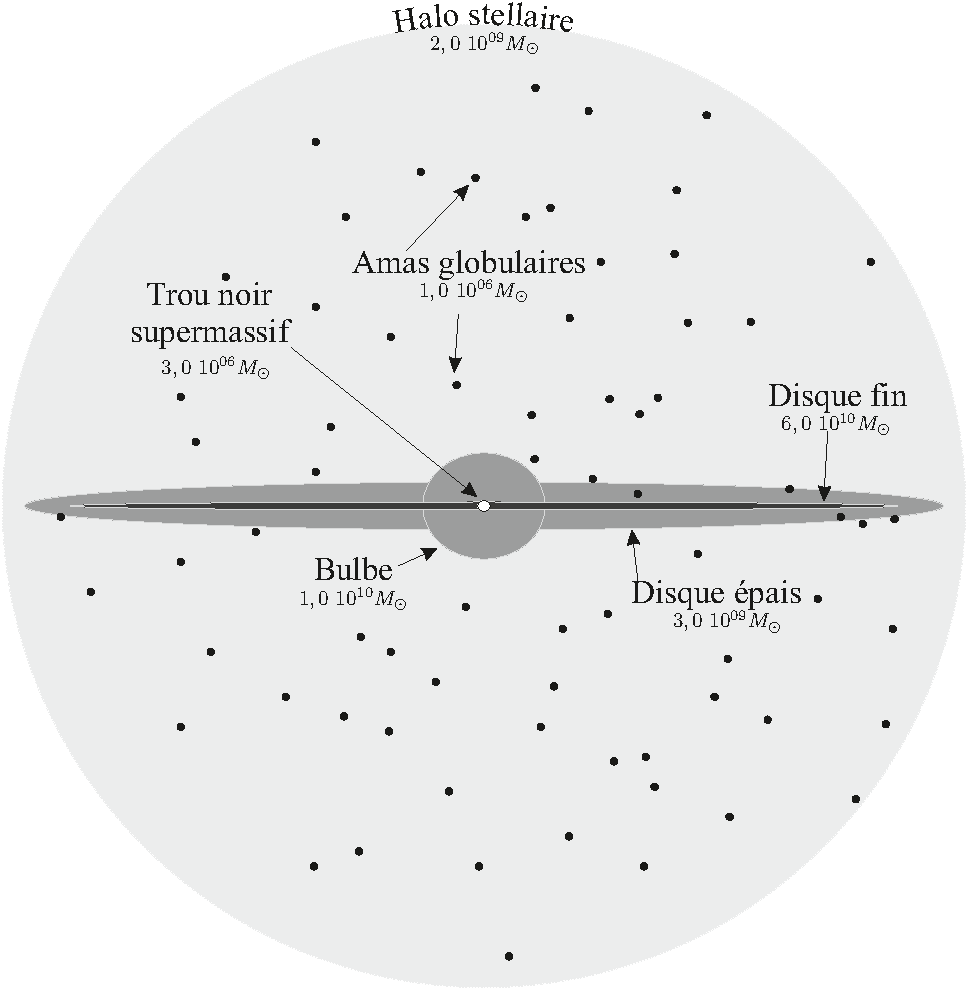
\includegraphics[scale=0.5]{voielactee}
				\end{center}
				\caption{Structure visible d'une galaxie spirale (figure extraite de~\citet{CoursJP}).\label{Fig::Intro::schemaGS}}
			\end{figure}

			% Et enfin les galaxies elliptiques qui sont généralement les
			La dernière classe principale est celle des galaxies elliptiques. Ces galaxies sont essentiellement
			constituées d'étoiles vieilles et ne contiennent que très
			peu de gaz.

		\subsection{Profils de matière noire}

			% Merrit et al
			\cite{2006AJ....132.2685M,2006AJ....132.2701G,2006AJ....132.2711G}
			ont menés une étude exhaustive des profils de matière
			noire dont la distribution a pu être mise en évidence
			autour des galaxies et dans les simulations numériques.

			Il ressort de cette étude qu'il n'existe pas réellement de profil universel, contrairement à ce qu'il fut suggéré par les travaux de la fin du \romannumeral 20
			\textsuperscript{e}~siècle (voir par exemple~\cite{NFW+97}). Chaque halo de matière noire pour chaque
			type de galaxie doit être ajusté par un profil différent. Comme nous l'avons vu plus haut, les galaxies naines ont un profil
			de type cœur-halo, et ce sont les seules à posséder un cœur. Les galaxies spirales et elliptiques possèdent généralement un profil
			montrant un cusp à la place du cœur (un profil de type cupside) ajusté correctement par un profil de Vaucouleurs.
			% correctement par un profil dit de Dehnen-McLaughin. Ce profil est directement issu d'une généralisation du profil de
			% Vaucouleurs: le profil de Einasto $R^{1/N}$.

			%ont une préférence pour les profil cupsy de Prugniel \&
			%Simien ou encore Dehnen-McLaughlin.

			Dès 1948, Gérard de Vaucouleurs remarqua que de nombreuses galaxies elliptiques possédaient une
			brillance de surface projetée variant comme:
			\begin{align}
				I(R) = I_\mathrm{eff} 10^{-3.3307\left[\(\dfrac{R}{R_\mathrm{eff}}\)^{1/4} - 1\right]}
			\end{align}
			avec $R$ le rayon projeté.
			C'est la fameuse loi de de Vaucouleurs. Depuis de nombreux modèles ont étendu celle-ci:
			\begin{itemize}
				\item le modèle empirique d'Einasto~\footnote{Ce modèle est bel et bien empirique car il est obtenu directement en
					remplaçant la brillance par la densité sans aucun calcul.} qui propose une densité volumique de masse de la
					forme:
					\begin{align}
						\rho(r) = \rho_e \exp\left[-d_n\left\{\(\dfrac{r}{r_e}\)^{1/n} - 1\right\}\right] \label{Intro::Eq::Einasto}
					\end{align}
					avec $\rho_e = \rho(r_e)$ et $r_e$ le rayon à 50\% de masse;
				\item le modèle de Prugniel-Simien, moins empirique que le précédent, est obtenu en déprojetant partiellement la loi de de
					Vaucouleurs, la densité est de la forme:
					\begin{align}
						\rho(r) = \rho_0\(\dfrac{r}{R_e}\)^{-p_n}\exp\left[-b_n\left\{\(\dfrac{r}{R_e}\)^{1/n}-1\right\}\right].\label{Intro::Eq::P-S}
					\end{align}
			\end{itemize}

			% Les profils des structures formées à l'échelle
			Les profils de matière noire formés à l'échelle
			galactique dans les simulations numériques sont quelque
			peu différents. En première approximation, le modèle
			NFW, couramment utilisé, convient. Mais les études plus
			fines menées par \cite{2006AJ....132.2685M,2006AJ....132.2701G,2006AJ....132.2711G} montrent que
			les profils de de Vaucouleurs généralisé~\ref{Intro::Eq::Einasto} et~\ref{Intro::Eq::P-S} conviennent mieux.
			% Einasto (issu d'une déprojection d'une brillance de
			% surface projetée en $R^{1/N}$) convient mieux. Ce
			% profil est issu de la même famille que les modèle de
			% Prugniel-Simien et Dehnen-McLaughin.

			%Pour les simulations numériques, c'est un peu
			%différent; de par sa simplicité les gens préfère
			%utiliser le profil de Navarro-Frenk-White, NFW. Or, et
			%cela est démontré dans la série d'article, le meilleur
			%profil pour les halos de matière noire est le Einasto
			%$R^{1/N}$.

		\subsection{Scénario de formation}
			Le scénario de formation des galaxies le plus généralement admis aujourd'hui est le scénario
			hiérarchique. Dans ce scénario, les plus petites structures, comme les galaxies naines, ont
			été les premières à se former. Puis, au fil des interactions, elles fusionnent pour former
			des structures de plus en plus grosses. Ainsi arrivent les galaxies spirales, puis
			elliptiques.

			% Cependant, ce modèle apporte son lot de problème. Notamment, il prévoit que les halos de matière
			% noire soit des cupsides là où les observations trouvent des cœur-halo, ou encore la quantité de
			% petite structure, tel les amas globulaire et les LSB, qui devrait être beaucoup plus importante autour de
			% notre galaxie.

			Cependant, ce modèle apporte son lot de problème:
			\begin{itemize}
				\item les simulations mettant en jeu ce processus montrent des profils de type cupside pour les halos de matière noire
					% il prévoit une structure de type cupside pour les halos de matière noire
					alors que les observations montrent que les galaxies naines possèdent un cœur et un halo et qu'elles sont très
					nombreuse;
				\item dans les modèles numériques de formation hiérarchique, le nombre de petites
					structures (amas globulaire et LSB) est beaucoup plus important que dans les
					observations (voir \citet{2006CombesBook} et les nombreuses références contenues dans ce livre).
				% \item la quantité de petite structure, tel les amas globulaire et les LSB, qui devrait
					% être beaucoup plus importante autour de notre galaxie.
			\end{itemize}

			Ces problèmes sont observés dans les simulations de formation de grande structures. Très peu d'études théoriques peuvent être
			menées sur ces échelles spatiales et temporelles. Nous pouvons cependant envisager certaines situations théoriques dans
			lesquelles certains aspects de ces problèmes peuvent être étudiés. C'est l'objet de la prochaine partie.


	\part{Théorie}
%		\minitoc
		\chapter{Temps caractéristiques et équation de Vlasov\label{Chap::TempsCarac}}
	\minitoc

	\section{Temps caractéristiques\label{chap_trelax}}

Les systèmes autogravitants possèdent plusieurs temps caractéristiques dont la connaissance est importante pour comprendre la dynamique.

\subsection{Le temps de croisement et le temps dynamique}

% Le temps de croisement $T_{cr}$ d'un système physique est défini comme le rapport d'une vitesse caractéristique par une taille caractéristique. La
% vitesse $V$ est par exemple celle d'un constituant représentatif du système, ou une dispersion de vitesse $\sigma=\sqrt{\left\langle
% V^{2}\right\rangle}$:
Pour un système quelconque, le temps de croisement est défini comme le temps caractéristique que mettrait une particule à parcourir le système dans son ensemble. Il est défini
comme le rapport entre une taille caractéristique et une vitesse caractéristique du système, typiquement la dispersion de vitesse du système $\sigma=\sqrt{\left\langle v^2\right\rangle}$:
\begin{align*}
	T_{cr}\propto\frac{R}{\sigma}%
\end{align*}
Le temps dynamique correspond au temps de croisement pour un système autogravitant isolé à l'équilibre. Le théorème du viriel donne:
\begin{align*}
	2E_{c}+E_{p}=0
\end{align*}
Pour un système de taille caractéristique $R$ composé de $N$ particules de masse $m$ et dont la dispersion de vitesse est $\sigma$ nous pouvons écrire:
\begin{align*}
	E_{c}=\frac{1}{2}Nm\sigma^{2}\ \ \ \text{et\ \ \ }E_{p}=-\frac{G\left(Nm\right)^{2}}{R}%
\end{align*}
le viriel donne donc:
\begin{align*}
	\sigma=\left(  \frac{GNm}{R}\right)  ^{1/2}=\left(  \frac{GM}{R}\right) ^{1/2}%
\end{align*}
En remplaçant la dispersion de vitesse $\sigma$ dans le temps de croisement par ce résultat, nous obtenons le temps dynamique:
\begin{align*}
	T_{d}\propto\sqrt{\frac{R^{3}}{GM}}%
\end{align*}
Le rapport $R^{3}/M$ est proportionnel à l'inverse de la densité moyenne de masse $\overline{\rho}$ du système, nous avons alors:
\begin{align}
	T_{d}\propto\left(  G\overline{\rho}\right)  ^{-1/2} \label{def:T-dyn_tcr} % \propto T_{cr}
\end{align}

Le problème de la relation~\refeq{def:T-dyn_tcr} est la définition précise de la densité moyenne. Si l'on se contente d'un ordre de grandeur pour $T_d$,
la question ne se pose pas mais pour l'analyse précise de simulation il faudra faire un choix. Nous aurons l'occasion d'y revenir dans la
section~\ref{Sec::2ndStudy} du chapitre~\ref{Chap::Resultat}.
Une option est de se donner un potentiel ou une répartition de masse et de calculer $\bar{\rho}$. % dans un sens statistique.
Nous pouvons alors écrire l'équation du mouvement d'une particule test à l'intérieur du système.
% Plusieurs temps caractéristiques apparaissent alors:
% \begin{itemize}

	% \item le temps de chute libre est celui pris par une particule pour rejoindre le centre depuis le bord du système;

	% \item le temps orbital est celui mis par une particule pour effectuer une période de son mouvement radial.

% \end{itemize}

% Tous ces temps sont de l'ordre de grandeur de $T_{d}$.

\subsection{Le temps de relaxation à deux corps}

Considérons un système constitué de $N$ particules ponctuelles de masse $m$ avec $N\gg1$. À l'équilibre, et sur de petites échelles de temps (de
l'ordre de $T_{d})$, il semble intéressant de considérer que l'une de ces particules soit en orbite dans le champ moyen créé par toutes les autres. Sur
de plus longues échelles de temps, le passage proche d'une voisine va affecter la trajectoire et modifier la vitesse de cette
particule test. Nous définissons donc le temps de relaxation à 2 corps comme:
\begin{align}
	T_{rel}\propto\left[  \overline{\frac{1}{v^{2}}\left(  \frac{dv^{2}}{dt}\right)  }\right]  ^{-1}. \label{TREL}%
\end{align}
Il s'interprète classiquement comme le temps mis par les interactions à 2 corps\footnote{Les interactions à plus de 2 corps sont négligeables.} pour modifier significativement
$v^{2}$. Le calcul de ce temps ainsi que des définitions plus précises abondent dans la littérature (voir par exemple le chapitre 14 de\ \cite{HH}),
nous privilégions ici l'extraction d'un ordre de grandeur basé sur un raisonnement de S. Chandrasekhar.

Tous les corps ont la même masse $m$. Lors d'un passage à une distance $p$ d'un voisin, une particule test de vitesse $v$ ressent une force de module:
\begin{align*}
	F=\frac{Gm^{2}}{p^{2}}%
\end{align*}
pendant un temps caractéristique:
\begin{align*}
	\delta\tau=\frac{p}{v}
\end{align*}
La variation de vitesse $\delta v$ de la particule test induite par cette rencontre peut s'obtenir en utilisant le principe fondamental de la dynamique:
\begin{align}
	m\frac{\delta v}{\delta\tau}=F\Rightarrow\delta v=\frac{F\delta\tau}{m}=\frac{Gm}{pv} \label{deltavrel}
\end{align}
Le paramètre $p$ est souvent appelé paramètre d'impact de la rencontre qui prend alors le statut de collision. Supposons que la particule test soit
en orbite circulaire de rayon $r$ dans le système de densité $\rho$. Sur une période, le nombre de collisions avec
un paramètre d'impact compris entre $p$ et $p+dp$ s'écrit:
\begin{align}
	dn  &= \left(  2\pi pdp\right)  \times\left(  2\pi r\right)  \times\left(\frac{\rho\left(  r\right)  }{m}\right) \label{dnrel}\\
	    &= \frac{4\pi^{2}}{m}pr\rho\left(  r\right)  dp
\end{align}
Les collisions sont suffisamment aléatoires pour que la moyenne des variations de vitesse $\overline{\delta v}$ soit nulle. Pour obtenir l'action des
collisions sur la vitesse, il faut donc considérer une dispersion de vitesse. Sur une période, la variation $\left(\Delta v^{2}\right)_{orb}$ de
$\delta v^{2}$ s'obtient en combinant~\refeq{deltavrel} et~\refeq{dnrel} et en sommant sur toutes les valeurs possibles de $p$, soit:
\begin{align*}
	\left(\Delta v^{2}\right)_{orb}=\int_{p_{\min}}^{p_{\max}}\delta v^{2}dn=\frac{4\pi^{2}G^{2}mr\rho\left(r\right)}{v^{2}}\int_{p_{\min}}^{p_{\max}}\frac{dp}{p}
\end{align*}
Si l'on veut éviter les infinis, il est nécessaire à ce stade d'introduire une coupure haute et basse pour les valeurs de $p$. Avec nos ordres de
grandeurs et en suivant le calcul de S. Chandrasekhar, nous introduisons le logarithme coulombien:
\begin{align*}
	\ln\Lambda=\ln\left(\frac{p_{\max}}{p_{\min}}\right)
\end{align*}
où $p_\mathrm{max}$ et $p_\mathrm{min}$ vont être des grandeurs caractéristiques du système.
% et utiliseront le fait que $p_{\max}=r$ tandis que $p_{\min}$ peut correspondre au rayon d'une particule test.
% que nous estimons par la relation crue%
% \begin{align*}
	% p_{\min}=\left(\frac{\frac{4}{3}\pi r^{3}}{N}\right)^{1/3}=\left(\frac{4\pi}{3N}\right)  ^{1/3}r
% \end{align*}
% ainsi%
% \begin{align*}
	% \ln\Lambda &=-\frac{1}{3}\ln\left(  \frac{4\pi}{3N}\right)=-\frac{1}{3}\left[\ln\left(\frac{4\pi}{3}\right)-\ln\left(N\right)\right] \\
	     % &\approx\frac{1}{3}\ln N
% \end{align*}
Finalement, sur une période nous obtenons:
\begin{align*}
	\left(\Delta v^{2}\right)_{orb}=4\pi^{2}\frac{G^{2}mr\rho\left(r\right)}{v^{2}}\ln \Lambda
\end{align*}
% Toujours sur une période nous avons vu au paragraphe précédent que:
Le temps dynamique étant à peu près le temps que met une particule à parcourir son orbite, nous pouvons écrire:
\begin{align*}
	\left(  \Delta t\right)  _{orb}\approx T_{d}%
\end{align*}
Ce qui nous permet d'écrire:
% il n'en faut pas plus pour écrire%
\begin{align*}
	\frac{1}{v^{2}}\left(\frac{dv^{2}}{dt}\right)_{orb}\approx4\pi^{2}\frac{G^{2}mr\rho\left(r\right)}{v^{4}}\frac{\ln \Lambda}{T_{d}}%
\end{align*}
La moyenne permettant de calculer le temps de relaxation à 2 corps peut s'envisager sur une période, l'expression~\refeq{TREL} s'écrit donc:
\begin{align*}
	\frac{T_{rel}}{T_{d}}\approx\frac{1}{4\pi^{2}}\frac{v^{4}}{G^{2}mr\rho\left(  r\right)  }\frac{1}{\ln \Lambda}%
\end{align*}
le théorème du viriel, car nous sommes à l'équilibre, nous donne:
\begin{align*}
	v^{4}=\left(\frac{GNm}{r}\right)^{2}%
\end{align*}
ainsi:
\begin{align*}
	\frac{T_{rel}}{T_{d}}\approx\frac{1}{4\pi^{2}}\frac{m}{r^{3}\rho\left(r\right)}\frac{N^{2}}{\ln \Lambda}
\end{align*}
% Au point où nous en sommes on peut toujours tenter
Nous écrivons:
\begin{align*}
	\rho\left(r\right)=\frac{Nm}{\frac{4}{3}\pi r^{3}}%
\end{align*}
et nous obtenons finalement:
\begin{align*}
	\frac{T_{rel}}{T_{d}}\approx\frac{3}{16\pi^{3}}\frac{N}{\ln \Lambda}%
\end{align*}
Dans un amas d'étoiles ou une galaxie, le temps de relaxation à deux corps est donc généralement beaucoup plus grand que le temps dynamique. Le
tableau~\ref{Tab::TempsCarac::OG} donne un ordre de grandeur de ces temps pour différents objets. %résume bien l'affaire
\begin{table}[htbp]
	\centering \begin{tabular}[c]{l|c|c|c|c|c|}
		\cline{2-6} & $N$ & $R\left[  \text{kpc}\right]  $ & $\sigma\left[  \text{km.s}^{-1}\right]$ & $T_{dyn}\left[  \text{Gan}\right]  $ & $T_{rel}\left[\text{Gan}\right]$\\\hline
		\multicolumn{0}{|l|}{\small {Amas ouverts}} & $250$ & $1\times10^{-3}$ & $1$ & $1\times10^{-3}$ & $8\times10^{-4}$\\\hline
		\multicolumn{0}{|l|}{\small {Amas globulaires}} & $5\times10^{5}$ & $1\times10^{-2}$ & $7$ & $1\times10^{-3}$ & $1$\\\hline
		\multicolumn{0}{|l|}{\small {Galaxies elliptiques}} & $10^{11}$ & $5$ & $200$ & $2\times10^{-2}$ & $2\times10^{6}$\\\hline
		\multicolumn{0}{|l|}{\small {Groupes diffus de galaxies}} & $5$ & $400$ & $100$ & $4$ & $2\times 10^{-1}$\\\hline
		\multicolumn{0}{|l|}{\small {Groupes compacts de galaxies}} & $4$ & $40$ & $200$ & $2\times 10^{-1}$ & $1\times10^{-2}$\\\hline
		\multicolumn{0}{|l|}{\small {Amas riches de galaxies}} & $400$ & $1200$ & $700$ & $2$ & $2$\\\hline
	\end{tabular}
	\caption{Ordres de grandeur des temps dynamiques et temps de relaxation à 2 corps pour divers objets.\label{Tab::TempsCarac::OG}}
\end{table}
Avec un univers âgé de $13$ Gan, les galaxies sont très peu influencées par les collisions à deux corps % les galaxies sont loin d'avoir acquis le statut d'objet relaxé par les collisions,
l'hypothèse Vlasov
est donc entièrement justifiée. En ce qui concerne les autres objets autogravitants, il est clair que les amas ouverts relaxent très vite alors que le
statut des amas globulaires est plus discutable: l'importance des collisions dans leur dynamique est différente entre les régions centrales denses et
le halo externe plus diffus.

Notons que le calcul du temps de relaxation à deux corps que nous avons présenté ici est sous-estimé en ce qui concerne les groupes et amas de galaxies,
pour lesquels l'effet de la matière noire doit être pris en compte.

Un phénomène de ségrégation de masse est associé au processus de collision. Une fois encore, ce calcul ne le prend pas en compte. Une rencontre
entre deux étoiles de masses différentes ne produit pas la même variation de vitesse. L'effet net de cette ségrégation est de ralentir les étoiles
les plus lourdes et donc de les faire tomber dans le puits de potentiel formé par le système. Sur l'échelle de temps de la relaxation, nous devrions
observer une organisation des objets dans le système: les plus lourds au centre, les plus légers à l'extérieur.

Dans le cadre de simulations numériques, l'estimation du temps de relaxation est une véritable question. Les valeurs de $p_{\min}$ et $p_{\max}$
utilisées pour le calcul du logarithme coulombien $\ln \Lambda$ doivent s'adapter à la simulation tout comme l'estimation de la densité. Nous
présenterons notre stratégie en la matière dans la section~\ref{Sec::2ndStudy} du chapitre~\ref{Chap::Resultat}.


	% \chapter{Le système de Vlasov-Poisson}

\section{Le système de Vlasov-Poisson}

\subsection{L'équation de Poisson}

%%%%%%%%%%%%%%%%%%%%%%%%%%%%%%%%%%%%%%%%%%%%%%%%%%%%%%%%%%%%%%%%%%%%%%%%%%%%%%%%%%%%%%%%%%%%%%%%%%%%%%%%%%%


Les systèmes que nous étudions en dynamique stellaire possèdent des tailles caractéristiques de l'ordre du parsec pour les amas globulaires et du
millier de parsecs pour les galaxies. En négligeant le rôle du gaz interstellaire et sur de telles échelles, la seule des quatre interactions pouvant
intervenir dans la dynamique de ces systèmes est la gravitation.

Nous considérons donc un système $\Omega\subset\mathbb{R}^{3}$ dont la masse est distribuée selon une certaine densité:
\begin{align*}
	\rho = \begin{cases}
		\rho(\vec{r}^{\,\prime}) & \text{si } \vec{r}^{\,\prime}\in\Omega\\
		0 & \text{si } \vec{r}^{\,\prime}\notin\Omega
	\end{cases}
	% \rho=\left\{
		% \begin{array}[c]{l}%
			% \rho(\vec{r}^{\,\prime})\\
			% 0
		% \end{array}%
		% \begin{array}[c]{l}%
			% \text{si}\qquad\vec{r}^{\,\prime}\in\Omega\\
			% \text{si}\qquad\vec{r}^{\,\prime}\notin\Omega
		% \end{array}
	% \right\}
\end{align*}
La loi de la gravitation de Newton nous indique alors que la force $\vec{f}(\vec{r})$ que crée le système en tout point
$\vec{r}\in\mathbb{R}^{3}$ de masse unité, est obtenue en sommant toutes les contributions infinitésimales:
\begin{align}
	\delta\vec{f}(\vec{r})=G\frac{\vec{r}^{\,\prime}-\vec{r}}{\left\vert\vec{r}^{\,\prime}-\vec{r}\right\vert ^{3}}\rho(\vec{r}^{\,\prime}%
	)\delta^{3}\vec{r}^{\,\prime}\label{poisss}%
\end{align}
issues de chaque élément de volume $\delta^{3}\vec{x}^{\,\prime}$. Dans l'hypothèse d'une distribution continue de matière nous avons donc:
\begin{align}
	\vec{f}(\vec{r})=G\displaystyle\int\frac{\vec{r}^{\,\prime}-\vec{r}}{\left\vert \vec{r}^{\,\prime}-\vec{r}\right\vert ^{3}}\rho
	(\vec{r}^{\,\prime})d^{3}\vec{r}^{\,\prime}\label{eq1}%
\end{align}

En introduisant le potentiel gravitationnel:
\begin{align}
	\psi(\vec{r})=-G\displaystyle\int\frac{\rho(\vec{r}^{\,\prime})}{\left\vert \vec{r}^{\,\prime}-\vec{r}\right\vert }d^{3}\vec{r}%
	^{\,\prime}\label{eq2}%
\end{align}
et en remarquant que:
\begin{align*}
	\mathrm{grad}_{\vec{r}}\left(  \frac{1}{\left\vert \vec{r}^{\,\prime}-\vec{r}\right\vert }\right)  =\frac{\vec{r}^{\,\prime}-\vec{r}%
	}{\left\vert \vec{r}^{\,\prime}-\vec{r}\right\vert ^{3}}
\end{align*}
Nous avons donc:
\begin{align*}
	\vec{f}(\vec{r})=G\displaystyle\int\mathrm{grad}_{\vec{r}}\left(\frac{1}{\left\vert \vec{r}^{\,\prime}-\vec{r}\right\vert }\right)
	\rho(\vec{r}^{\,\prime})d^{3}\vec{r}^{\,\prime}
\end{align*}
pour une large classe de densités suffisamment régulières (celles permettant à~\ref{eq1} de converger), la force dérive donc du potentiel~\ref{eq2} et
nous avons:
\begin{align}
	\vec{f}(\vec{r})=-\mathrm{grad}_{\vec{r}}\psi(\vec{r})\label{eq3}%
\end{align}
le système est alors dit conservatif. Plutôt que d'utiliser le champ vectoriel $\vec{f}(\vec{r})$, il est préférable de trouver une relation
entre champs scalaires. Ceci est possible en remarquant que l'équation~\ref{eq2} est une convolution:
\begin{align}
	\psi(\vec{r},t)=-G\,\,\,\rho(\vec{r},t)\ast\frac{1}{\left\vert\vec{r}\right\vert }\ .\label{poiconvlap}%
\end{align}
La deuxième fonction de cette convolution est, à une constante près, la fonction de Green du laplacien. Un calcul montre en effet que si
$u$ est une fonction test au sens des distributions, alors le produit scalaire:
\begin{align*}
	\left\langle \Delta\left(  \frac{1}{\left\vert \vec{r}\right\vert }\right),u\right\rangle =-4\pi\,u\left(  0\right)  =\left\langle -4\pi\delta\left(
	\vec{r}\right)  \text{ },u\right\rangle\text{.}
\end{align*}
Nous allons donc appliquer le laplacien à l'équation~\ref{poiconvlap} qui s'écrit alors:
\begin{align*}
	\left\langle \Delta\psi(\vec{r},t),u\right\rangle =\left\langle-G\,\,\Delta\left(  \rho(\vec{r},t)\ast\frac{1}{\left\vert \vec{r}%
	\right\vert }\right),u\right\rangle
\end{align*}
soit:
\begin{align*}
	\left\langle \Delta\psi(\vec{r},t),u\right\rangle =\left\langle-G\,\,\rho(\vec{r},t)\ast\Delta\left(  \frac{1}{\left\vert \vec{r}%
	\right\vert }\right)  ,u\right\rangle =\left\langle 4\pi G\,\,\rho(\vec{r},t)\ast\delta\left(  \vec{r}\right)  ,u\right\rangle
\end{align*}

Le Dirac étant l'élément neutre de l'algèbre de convolution, nous obtenons finalement l'équation de Poisson:
\begin{align*}
	\Delta\psi(\vec{r},t)=4\pi G\,\,\rho(\vec{r},t)
\end{align*}

Cette équation, seule ou couplée avec d'autres, est à la base de nombreux problèmes d'astrophysique théorique.

\begin{itemize}

	\item Utilisée seule elle nécessite la donnée (théorique ou expérimentale) de la fonction $\rho(\vec{r})$. La résolution de l'équation de
		Poisson fournit alors la force générée par le système en tout point de l'espace, il devient donc formellement possible de
		connaître les propriétés dynamiques de la trajectoire d'une particule test évoluant dans le champ de gravitation créé par la
		distribution $\Omega$.

	\item Dans le cadre d'une théorie fournissant la densité du système, l'équation de Poisson sera alors utilisée comme équation de fermeture
		du problème.

\end{itemize}

\subsection{L'équation de Vlasov}

Pour étudier la dynamique des systèmes autogravitants comme les galaxies ou les amas globulaires, la mise en œuvre des méthodes de la mécanique
classique conduit à écrire, donc à résoudre, un nombre d'équations différentielles égal au nombre d'étoiles composant le système, ce qui est en
pratique irréalisable.\ Il convient d'utiliser des méthodes statistiques de champ moyen, dans le cas gravitationnel la théorie de Vlasov-Poisson.

Supposons que le système que nous considérons possède $3N$ degrés de liberté. Cela signifie que les positions des différents points du système sont
définies par $N$ vecteurs $\vec{r}_{\alpha}$ comportant chacun 3 composantes, l'indice $\alpha$ prenant toutes les valeurs $1,2,\cdots,N$. À un
instant donné, l'état du système sera complètement déterminé par les $N$ vecteurs position et les $N$ vecteurs impulsion
$\vec{p}_{\alpha}=m_{\alpha}\vec{\dot{r}}_{\alpha}$ correspondants. On peut représenter mathématiquement les différents états d'un système par
des points dans un espace à $6N$ {dimension}s appelé espace des phases. La trajectoire, ou le lieu de ces points, permet de représenter de manière
univoque l'évolution du système.

En s'intéressant à un volume infinitésimal $d\Gamma$ de cet espace des phases:
\begin{align*}
	d\Gamma:=d\vec{r}_{1}d\vec{r}_{2}\cdots d\vec{r}_{N}d\vec{p}_{1}d\vec{p}_{2}\cdots d\vec{p}_{N}
\end{align*}
nous pouvons introduire la probabilité $d\Omega$ des états représentés par des points contenus dans ce volume à l'instant $t$. C'est-à-dire, la probabilité
pour qu'à cet instant les positions $\vec{r}_{\alpha}$ et les {impulsion}s $\vec{p}_{\alpha}$ soient comprises dans les intervalles
infinitésimaux $[\vec{r}_{\alpha }+d\vec{r}_{\alpha}]$ et $[\vec{p}_{\alpha}+d\vec{p}_{\alpha}]$. Cette probabilité s'exprime
par:
\begin{align*}
	d\Omega\;=\;f^{(N)}(\vec{r}_{1},\cdots,\vec{r}_{N},\vec{p}_{1},\cdots,\vec{p}_{N},t)\,d\Gamma
\end{align*}
où la quantité $f^{(N)}(\vec{r}_{1},\cdots,\vec{r} _{N},\vec{p}_{1},\cdots,\vec{p}_{N},t)$ est appelée fonction de distribution à $N$
particules du système. Cette fonction est positive et de norme unité:
\begin{align*}
	1=\int f^{\left(N\right)}\left(\vec{w}_{1},...,\vec{w}_{N},t\right)d\vec{w}_{1}\,...d\vec{w}_{N}
\end{align*}
Elle représente la densité, au sens probabiliste, de la variable aléatoire $\vec{w}=(\vec{w}_{1},...,\vec{w}_{N})$ avec
$\vec{w}_{\alpha}=\left(  \vec{r}_{\alpha},\vec{p}_{\alpha}\right) $. Si le nombre de particules est conservé au cours de l'évolution, cette
densité obéit à une équation de continuité (exprimant le fait que $df$ est une différentielle totale exacte, ou physiquement que le nombre de
particules est conservé):
\begin{align}
	\frac{\partial f^{(N)}}{\partial t}\;+\;\mathrm{div}_{\vec{w}}(f^{(N)}\vec{\dot{w}})\;=\;0\label{continu}%
\end{align}
où $\vec{\dot{w}}=(\vec{\dot{r}}_{1},\vec{\dot{p}}_{1} ,...,\vec{\dot{r}}_{N},\vec{\dot{p}}_{N})$ représente la vitesse du flot des
points dans l'espace des phases. En explicitant la divergence de l'équation~\ref{continu}, il vient:
\begin{align*}
	\frac{\partial f^{(N)}}{\partial t}\;+\;\sum_{\alpha=1}^{N}\left[\mathrm{div}_{\vec{r}_{\alpha}}\left(  f^{(N)}\vec{\dot{r}}_{\alpha
	}\right)  +\mathrm{div}_{\vec{p}_{\alpha}}\left(  f^{(N)}\vec{\dot{p}}_{\alpha}\right)  \right]=0
\end{align*}
Après dérivation, nous obtenons:
\begin{align*}
	&  \frac{\partial f^{(N)}}{\partial t}+\displaystyle\sum\limits_{\alpha=1}%
	^{N}\left\{  \vec{\dot{r}}_{\alpha}.\mathrm{grad}_{\vec{r}_{\alpha}%
	}\left(  f^{(N)}\right)  +\vec{\dot{p}}_{\alpha}.\mathrm{grad}%
	_{\vec{p}_{\alpha}}\left(  f^{(N)}\right)  \right. \\
	&  \,\;\;\;\;\;\;\;\left.  +~f^{(N)}\left[  \mathrm{div}_{\vec{r}_{\alpha}%
	}\left(  \vec{\dot{r}}_{\alpha}\right)  +\mathrm{div}_{\vec{p}_{\alpha}%
	}\left(  \vec{\dot{p}}_{\alpha}\right)  \right]  \right\}=0
\end{align*}
Nous introduisons alors les équations de Hamilton pour chaque particule (qui reviennent ici à écrire le principe fondamental de la dynamique):
\begin{align*}
	\forall~1\leq\alpha\leq N~~~~\vec{\dot{r}}_{\alpha}=\frac{\partial H}{\partial\vec{p}_{\alpha}}~~~~\text{et}~~~~\vec{\dot{p}}_{\alpha
	}=-\frac{\partial H}{\partial\vec{r}_{\alpha}}
\end{align*}
où $H$ est le hamiltonien du système:
\begin{align*}
	\begin{array}[c]{cccc}
		H= & \displaystyle\sum\limits_{\alpha=1}^{N}\dfrac{\vec{p}_{\alpha}^{2}}{2m_{\alpha}} & + & \displaystyle\sum\limits_{\alpha\neq\beta=1}^{N,N}%
		-\dfrac{G}{2}\dfrac{m_{\alpha}m_{\beta}}{\left\vert \vec{r}_{\alpha}-\vec{r}_{\beta}\right\vert }%
	\end{array}
\end{align*}
nous constatons alors que:
\begin{align*}
	\forall~1\leq\alpha\leq N~~~~\mathrm{div}_{\vec{r}_{\alpha}}\left(\vec{\dot{r}}_{\alpha}\right)  =\frac{\partial^{2}H}{\partial
	\vec{r}_{\alpha}\partial\vec{p}_{\alpha}}=-\mathrm{div}_{\vec{p}_{\alpha}}\left(  \vec{\dot{p}}_{\alpha}\right)
\end{align*}
Ainsi l'équation de continuité se met sous la forme:
\begin{align}
	\frac{\partial f^{(N)}}{\partial t}+\sum_{\alpha=1}^{N}\left[  \vec{\dot{r}}_{\alpha}.\mathrm{grad}_{\vec{r}_{\alpha}}\left(  f^{(N)}\right)
	+\vec{\dot{p}}_{\alpha}.\mathrm{grad}_{\vec{p}_{\alpha}}\left(f^{(N)}\right)  \right]  =0\label{liouville}%
\end{align}
Il s'agit de l'équation de Liouville.

Dans notre contexte gravitationnel, la forme du hamiltonien permet de
l'expliciter plus avant:
\begin{align*}
	\frac{\partial f^{(N)}}{\partial t}+\sum_{\alpha=1}^{N}\left\{  \dfrac{\vec{p}_{\alpha}}{m_{\alpha}}.\dfrac{\partial f^{(N)}}{\partial
	\vec{r}_{\alpha}}-\dfrac{\partial U_{\alpha}}{\partial\vec{r}_{\alpha}}.\dfrac{\partial f^{(N)}}{\partial\vec{p}_{\alpha}}\right\}  =0
\end{align*}
où nous avons posé:
\begin{align*}
	U_{1}=\displaystyle\sum\limits_{\beta=2}^{N}-G\dfrac{m_{1}m_{\beta}}{\left\vert \vec{r}_{1}-\vec{r}_{\beta}\right\vert }\ ,\ \ U_{2}%
	=-G\dfrac{m_{2}m_{1}}{\left\vert \vec{r}_{2}-\vec{r}_{1}\right\vert}+\displaystyle\sum\limits_{\beta=3}^{N}-G\dfrac{m_{1}m_{\beta}}{\left\vert
	\vec{r}_{2}-\vec{r}_{\beta}\right\vert }\ ,\ \ \ \text{etc...}
\end{align*}
En pratique, lorsque le système devient plus grand qu'une paire, cette équation s'avère inutilisable, et nous devons faire des hypothèses de nature
statistique. À partir de la fonction de distribution à $N$ particules $f^{(N)}$, nous pouvons construire une fonction de distribution à une particule
(densité marginale):
\begin{align*}
	f^{(1)}=f^{(1)}(\vec{w}_{1},t)=\int\cdots\int f^{(N)}d\vec{w}_{2}\cdots d\vec{w}_{N}
\end{align*}
En intégrant l'équation de Liouville sur $\vec{w}_{2}\cdots\vec{w}_{N}$, il vient:
\begin{align*}%
	\begin{array}[c]{ll}%
		\dfrac{\partial f^{(1)}}{\partial t} & +\displaystyle\sum\limits_{\alpha=1}^{N}\left\{  \displaystyle\int\dfrac{\vec{p}_{\alpha}}{m_{\alpha}%
		}.\dfrac{\partial f^{(N)}}{\partial\vec{r}_{\alpha}}d\vec{w}_{2}\cdots d\vec{w}_{N}\right\} \\
		& \\
		& -\displaystyle\sum\limits_{\alpha=1}^{N}\left\{  \displaystyle\int\dfrac{\partial U_{\alpha}}{\partial\vec{r}_{\alpha}}.\dfrac{\partial
		f^{(N)}}{\partial\vec{p}_{\alpha}}d\vec{w}_{2}\cdots d\vec{w}_{N}\right\}  =0
	\end{array}
\end{align*}
Les deux sommes d'intégrales se simplifient considérablement en utilisant le fait que la fonction de distribution s'annule sur le bord du système:
\begin{align*}
	\forall\alpha=1,...,N\qquad\lim_{\vec{w}_{\alpha}\rightarrow\infty}f^{\left(  N\right)  }=0
\end{align*}
ainsi toutes les intégrations sur $\vec{r}_{2},...,\vec{r}_{N}$ s'annulent et:
\begin{align*}%
	\begin{array}[c]{ll}%
		\displaystyle\sum\limits_{\alpha=1}^{N}\left\{  \displaystyle\int%
		\dfrac{\vec{p}_{\alpha}}{m_{\alpha}}.\dfrac{\partial f^{(N)}}%
		{\partial\vec{r}_{\alpha}}d\vec{w}_{2}\cdots d\vec{w}_{N}\right\}  &
		=\displaystyle\int\dfrac{\vec{p}_{1}}{m_{1}}.\dfrac{\partial f^{(N)}%
		}{\partial\vec{r}_{1}}d\vec{w}_{2}\cdots d\vec{w}_{N}\\
		& \\
		& =\dfrac{\vec{p}_{1}}{m_{1}}.\dfrac{\partial}{\partial\vec{r}_{1}%
		}\displaystyle\int f^{(N)}d\vec{w}_{2}\cdots d\vec{w}_{N}\\
		& \\
		& =\dfrac{\vec{p}_{1}}{m_{1}}.\dfrac{\partial f^{(1)}}{\partial
		\vec{r}_{1}}%
	\end{array}
\end{align*}

Pour les mêmes raisons mais en vitesse:
\begin{align*}%
	\begin{array}[c]{ll}%
		\displaystyle\sum\limits_{\alpha=1}^{N}\left\{  \displaystyle\int%
		\dfrac{\partial U_{\alpha}}{\partial\vec{r}_{\alpha}}.\dfrac{\partial
		f^{(N)}}{\partial\vec{p}_{\alpha}}d\vec{w}_{2}\cdots d\vec{w}%
		_{N}\right\}   & =\displaystyle\int\dfrac{\partial U_{1}}{\partial
		\vec{r}_{1}}.\dfrac{\partial f^{(N)}}{\partial\vec{p}_{1}}%
		d\vec{w}_{2}\cdots d\vec{w}_{N}%
	\end{array}
\end{align*}
% de l'équation de Liouville il ne reste alors plus que:
L'équation de Liouville devient alors:
\begin{align*}
	\frac{\partial f^{(1)}}{\partial t}+\dfrac{\vec{p}_{1}}{m_{1}}.\dfrac{\partial f^{(1)}}{\partial\vec{r}_{1}}-\displaystyle\int%
	\dfrac{\partial U_{1}}{\partial\vec{r}_{1}}.\dfrac{\partial f^{(N)}}{\partial\vec{p}_{1}}d\vec{w}_{2}\cdots d\vec{w}_{N}=0
\end{align*}
% L'hypothèse qu'il convient alors de faire est de supposer les particules indiscernables.
Nous allons maintenant supposer que les particules sont indiscernables.
Explicitons cette subtilité sur le calcul de l'énergie potentielle:
\begin{align*}
	U_{1} &  =U_{1}\left(  \vec{r}_{1},...,\vec{r}_{N}\right)  =\sum_{\beta=2}^{N}U_{1\beta}\\
	\intertext{où}
	U_{\alpha\beta} &  =U_{\alpha\beta}\left(  \vec{r}_{\alpha},\vec{r}_{\beta}\right)  :=-\frac{Gm_{\alpha}m_{\beta}}{\left\vert\vec{r}_{\alpha}-\vec{r}_{\beta}\right\vert }%
\end{align*}
Dans cette somme, l'indiscernabilité des particules fait jouer à toutes le même rôle. Nous pouvons donc en choisir une (la particule 1) pour représenter
toutes les autres et subir leur action globale, et une autre (la particule 2) pour représenter toutes les particules du système et agir sur la
particule 1 de façon globale. Il s'agit de l'hypothèse de champ moyen. Elle est fondamentale. En pratique cela revient à considérer que:
\begin{align*}
	U_{12}=U_{13}=\cdots=U_{1N}\ \ \ \Rightarrow\ U_{1}=\sum_{\beta=2}^{N}U_{1\beta}\ =\left(  N-1\right)  U_{12}
\end{align*}
ainsi l'intégrale devient:
\begin{align*}
	\displaystyle\int\dfrac{\partial U_{1}}{\partial\vec{r}_{1}}.\dfrac{\partial f^{(N)}}{\partial\vec{p}_{1}}d\vec{w}_{2}\cdots d\vec{w}%
	_{N}=\left(  N-1\right)  \displaystyle\int\dfrac{\partial U_{12}}{\partial\vec{r}_{1}}.\dfrac{\partial f^{(N)}}{\partial\vec{p}_{1}%
	}d\vec{w}_{2}\cdots d\vec{w}_{N}%
\end{align*}
La particule 1 est appelée \og\emph{particule test}\fg, elle évolue dans le système moyen représenté par la particule 2.

En introduisant la densité marginale à 2 particules:
\begin{align*}
	f^{(2)}=f^{(2)}(\vec{w}_{1},\vec{w}_{2},t)=\int\cdots\int f^{(N)}d\vec{w}_{3}\cdots d\vec{w}_{N}
\end{align*}
et comme $U_{12}$ ne dépend que de $\vec{w}_{1}$ et $\vec{w}_{2}$, on peut finir l'intégration du terme contenant l'énergie potentielle pour
obtenir la version intégrée de Liouville suivante:
\begin{align}
	\frac{\partial f^{(1)}}{\partial t}+\dfrac{\vec{p}_{1}}{m_{1}}.\dfrac{\partial f^{(1)}}{\partial\vec{r}_{1}}=\left(  N-1\right)
	\displaystyle \int\dfrac{\partial U_{12}}{\partial\vec{r}_{1}}.\dfrac{\partial f^{(2)}}{\partial\vec{p}_{1}}d\vec{w}_{2}%
	\label{liouint}%
\end{align}
Cette équation permet donc de calculer $f^{(1)}$ à partir de $f^{(2)}$, en poursuivant nous obtenons:
\begin{align*}
	f^{(1)}\hookleftarrow f^{(2)}\hookleftarrow...\hookleftarrow f^{(N)}
\end{align*}
Cette cascade d'équations est généralement appelée
hiérarchie BBGKY.

La technique habituelle consiste à stopper la hiérarchie, c'est-à-dire trouver dans quelles conditions:
\begin{align*}
	\exists p<N,\qquad\text{tel que \qquad}\forall n>p\qquad f^{\left(  n\right) }=0
\end{align*}


Dans ce contexte, l'hypothèse de chaos moléculaire de Boltzmann est utile, elle revient à poser:
\begin{align*}
	f^{(2)}(\vec{w}_{1},\vec{w}_{2},t)=f^{(1)}(\vec{w}_{1},t)f^{(1)}(\vec{w}_{2},t)+g(\vec{w}_{1},\vec{w}_{2},t)
\end{align*}
la fonction $g(\vec{w}_{1},\vec{w}_{2},t)$ décrivant les corrélations ou interactions binaires.

Les particules étant indiscernables, il convient de poser:
\begin{align*}
	f\left(  \vec{w},t\right)  =N\,f^{(1)}(\vec{w},t) \\
	\intertext{ainsi}
	\int f\left(  \vec{w},t\right)  d\vec{w=}N
\end{align*}
Sous toutes ces hypothèses, la version intégrée~\ref{liouint} de l'équation de Liouville s'écrit donc:
\begin{align*}
	\frac{\left(  \frac{\partial f}{\partial t}+\frac{\vec{p_{1}}}{m_{1}}.\frac{\partial f}{\partial\vec{r}}\right)  }{{\ N}}=\left(  {\ N-1}%
	\right)  \displaystyle\int\tfrac{\partial U_{12}}{\partial\vec{r}_{1}}.\frac{{\ \partial}\left(  \frac{f\left(  \vec{w}_{1},t\right)  }{N}%
	\frac{f\left(  \vec{w}_{2},t\right)  }{N}+{\ g}\right)  }{{\ \partial}\vec{p}_{1}}d\vec{w}_{2}%
\end{align*}
soit:
\begin{align*}%
	\begin{array}[c]{ll}%
		\dfrac{\partial f}{\partial t}+\dfrac{\vec{p_{1}}}{m_{1}}.\dfrac{\partial f}{\partial\vec{r}}= & \dfrac{\left(  N-1\right)  }{N}\dfrac{\partial
		f\left(  \vec{w}_{1},t\right)  }{\partial\vec{p}_{1}}\dfrac{\partial}{\partial\vec{r}_{1}}\displaystyle\int U_{12}f\left(  \vec{w}%
		_{2},t\right)  d\vec{w}_{2}\\
		& \\
		& +N\left(  N-1\right)  \displaystyle\int\dfrac{\partial U_{12}}{\partial\vec{r}_{1}}.\dfrac{\partial g}{\partial\vec{p}_{1}}%
		d\vec{w}_{2}%
	\end{array}
\end{align*}
un petit rappel s'impose alors:
\begin{align*}
	\displaystyle\int U_{12}f\left(  \vec{w}_{2},t\right)  d\vec{w}_{2}=-Gm_{1}m_{2}\displaystyle\int\dfrac{f\left(  \vec{w}_{2},t\right)
	}{\left\vert \vec{r}_{1}-\vec{r}_{2}\right\vert }d\vec{r}_{2}d\vec{p}_{2}%
\end{align*}
dans le second membre de cette relation, l'intégration sur les impulsions nous fait reconnaître la densité de masse:
\begin{align*}
	\rho\left(  \vec{r_{2}},t\right)  =m_{2}\displaystyle\int f\left(\vec{w_{2}},t\right)  d\vec{p}%
\end{align*}
Nous avons donc:
\begin{align*}
	\displaystyle\int U_{12}f\left(  \vec{w}_{2},t\right)  d\vec{w}_{2}=-Gm_{1}\displaystyle\int\dfrac{\rho\left(  \vec{r}_{2},t\right)
	}{\left\vert \vec{r}_{1}-\vec{r}_{2}\right\vert }d\vec{r}_{2}%
\end{align*}
où l'on voit sourdre le potentiel gravitationnel impliqué dans l'équation de Poisson:
\begin{align*}
	\displaystyle{\ \int U_{12}f\left(  \vec{w}_{2},t\right)  d\vec{w}_{2}=m_{1}\psi\left(  \vec{r}_{1},t\right)  }%
\end{align*}
en prenant $N-1\approx N$, et en laissant de côté l'indice 1 nous obtenons finalement
\begin{align}
	\frac{\partial f}{\partial t}+\frac{\vec{p}}{m}.\frac{\partial f}{\partial\vec{r}}-m\frac{\partial f}{\partial\vec{p}}\frac{\partial\psi
	}{\partial\vec{r}}=N^{2}GC\left(  \vec{w},t\right)  \label{boltzman}%
\end{align}
où nous avons introduit le terme de corrélation:
\begin{align*}
	C\left(  \vec{w},t\right)  =\displaystyle\int\dfrac{\partial g\left(\vec{w},\vec{w}_{2},t\right)  }{\partial\vec{p}}\dfrac{\vec{r}%
	-\vec{r}_{2}}{\left\vert \vec{r}-\vec{r}_{2}\right\vert ^{3}}d\vec{w}_{2}%
\end{align*}
L'équation~\ref{boltzman} est appelée équation de Boltzmann.

Dans le cas des systèmes gravitationnels, et contrairement au gaz de Van Der Waals, les collisions sont dynamiquement inefficaces pendant de longues
périodes, Chandrasekhar montre que pour un système autogravitant composé de $N$ particules, le temps dynamique $T_{d}$ et le temps de
relaxation par collisions $T_{rel}$ vérifient (voir~\ref{chap_trelax}):
\begin{align*}
	T_{rc}\approx N\ln\left(  N\right)  T_{d}%
\end{align*}
Sur une centaine de temps dynamiques, les amas globulaires et galaxies en tous genres sont dits non collisionnels, i.e. $C\left(  \vec{w}
,t\right)  \equiv0$, et l'équation de la dynamique des galaxies est l'équation de Vlasov (Boltzmann sans collisions):
\begin{align*}
	\dfrac{\partial f}{\partial t}+\dfrac{\vec{p}}{m}\ \dfrac{\partial f}{\partial\vec{r}}-m\dfrac{\partial f}{\partial\vec{p}}\dfrac
	{\partial\psi}{\partial\vec{r}}=0
\end{align*}
dans cette équation le potentiel $\psi$ est lui-même relié à la fonction de distribution $f$ via l'équation de Poisson, nous avons donc le système
intégro-différentiel suivant:
\begin{align*}
	\left\{
		\begin{array}[c]{l}%
			\dfrac{\partial f}{\partial t}+\dfrac{\vec{p}}{m}\ \dfrac{\partial f}{\partial\vec{r}}-m\dfrac{\partial f}{\partial\vec{p}}\dfrac
			{\partial\psi}{\partial\vec{r}}=0\\
			\\
			\psi(\vec{r},t\vec{)}=~-Gm\displaystyle\int\dfrac{f(\vec{r}^{\,\prime},\vec{p}^{\,\prime},t)}{\mid\vec{r}-\vec{r}^{\,\prime}\mid}%
			d^{3}\vec{r}^{\,\prime}d^{3}\vec{p}^{\,\prime}%
		\end{array}
	\right.
\end{align*}
dit système de Vlasov-Poisson, en introduisant l'énergie moyenne par particule:
\begin{align*}
	E=\frac{\vec{p}^{2}}{2m}+m\psi
\end{align*}
ce système s'écrit sous forme canonique:
\begin{align*}
	\left\{
		\begin{array}[c]{lll}%
			\dfrac{\partial f}{\partial t}=\left\{  \,E\,,\,f\,\right\}   &  & \text{{\ {Vlasov} : dynamique}}\\
			\Delta\psi=~4\pi G\rho &  & \text{{\ {Poisson} : champ {moyen}}}%
		\end{array}
	\right.
\end{align*}


Ce système est à la base de l'étude de la dynamique des galaxies. Nous proposons deux axes principaux d'études pour ce problème:
\begin{itemize}

	\item L'étude des solutions stationnaires du système de Vlasov-Poisson qui devrait nous permettre de rendre compte des diverses propriétés des
		galaxies lorsqu'elles peuvent être considérées en équilibre.

	\item L'étude de la stabilité des solutions stationnaires du système de Vlasov-Poisson afin de connaître les configurations d'équilibre
		privilégiées pour un système auto-gravitant.

\end{itemize}




\chapter{Le problème de la sphère isotherme}
		\minitoc
		
		\section{La sphère isotherme et son problème intrinsèque}
	La sphère isotherme est la solution classique fournie par une approche thermodynamique du problème de l'équilibre d'un système autogravitant.
	Elle apparait lorsque nous cherchons un maximum de l'entropie statistique de Boltzmann $S(f) = -k_B \int f\ln(f) d\vec{r}d\vec{p}$, où $k_B$ est la constante de Boltzmann.
	En imposant les contraintes d'une masse fixée:
	\begin{align}
		M = \int \rho(\vec{r},t) d\vec{r}
	\end{align}
	et une énergie totale fixée:
	\begin{align}
		H = \int \frac{\vec{p}\,^2}{2m} f d\vec{r}d\vec{p}-\frac{Gm^2}{2}\int \int 
		\frac{f(\vec{r},\vec{p})f(\vec{r}\,^{\prime},\vec{p}\,^{\prime})}
		      {\left|\vec{r}-\vec{r}\,^{\prime}\right|}
		d^3\vec{r}\,^{\prime}d^3\vec{p}\,^{\prime}
	\end{align}
	Pour le système sa fonction de distribution s'écrit :
	\begin{align}
		f(\vec{r},\vec{p})=f(E) = \(\frac{2\pi \alpha^2 m}{\beta}\)^{-3/2} e^{-\beta E}
		\label{sph-iso}
	\end{align}
	La fonction $E=\frac{\vec{p}\,^2}{2m}+m\psi(\vec{r})$ caractérise l'énergie d'une particule test.
	Les constantes $\beta = \frac{1}{k_B T}$ et $\alpha$ sont des multiplicateurs de \textsc{Lagrange} associés aux contraintes imposées lors de la recherche de l'extremum de l'entropie :
	$\beta \Leftrightarrow H = \mathrm{cte}$ et $\alpha \Leftrightarrow M = \mathrm{cte}$.

	Les différents problèmes posés par cette solution ont émaillé la recherche dans ce domaine tout au long du
	\textsc{xx}$^{e}$ siècle d'\cite{emden07} à \cite{1989ApJS...71..651P}  en passant par
	\cite{chandra39}, la revue de \cite{2006IJMPB..20.3113C} pourra être consulté à ce sujet.
	% on pourra consulter à ce sujet la revue de \cite{2006IJMPB..20.3113C}.
	Nous en reprendrons les éléments principaux.
	
\section{Formulation générale du problème}
	
	La densité de la sphère isotherme se calcule directement à partir de la définition \ref{sph-iso}:
	\begin{align}
		\rho(r) &= m \int \(\frac{2\pi \alpha^2 m}{\beta}\)^{-3/2} e^{-\beta \(\frac{p^2}{2m} + m\psi\)} d^3 p \notag \\
			&= 4\pi m \(\frac{2\pi \alpha^2 m}{\beta}\)^{-3/2} \int_0^\infty e^{-\beta \(\frac{p^2}{2m} + m\psi\)} p^2 dp \notag \\
			&= \frac{m}{\alpha^3} e^{-m\beta\psi}
	\end{align}
	Nous avons $\rho(\vec{r}) = \rho(\psi)$, le théorème Gidas-Ni-Niremberg s'applique (voir~\cite{CoursJP}) et le système est donc à symétrie sphérique $\rho(\vec{r}) = \rho(r)$  dans l'espace des positions.
	Avec cette symétrie radiale l'équation de Poisson s'écrit:
	\begin{align}
		\frac{1}{r^2}\frac{d}{dr}\(r^2\frac{d\psi(r)}{dr}\) &= 4\pi G \rho(r) = 4\pi G \frac{m}{\alpha^3} e^{-m\beta\psi(r)} \notag \\
		\intertext{En introduisant les variables $y = m\beta\psi$ et $x = r/r_0$, nous obtenons :}
		\frac{1}{x^2}\frac{d}{dx}\(x^2\frac{d y}{dx}\) &=  \frac{4\pi G m r_0^2}{\alpha^3} e^{-y} \notag \\
		\intertext{Nous pouvons alors choisir $r_0^2 = \frac{\alpha^3}{4\pi G m r_0^2}$ afin d'adimensionner l'équation de Poisson sous la forme:}
		\frac{1}{x^2}\frac{d}{dx}\(x^2\frac{d y}{dx}\) &= e^{-y} \label{Pois:sis}
	\end{align}
	
	Nous pouvons chercher dans un premier temps  des solutions autosimilaires pour cette équation, elles sont de la forme $\Tilde{y}$ telles que :
	\begin{align}
		\Tilde{\rho}(r) &= \frac{A}{r^2} = e^{-\Tilde{y}} \quad
		\Rightarrow \quad \Tilde{y} = - \ln\(\frac{A}{x^2}\)
	\end{align}
	Il est facile de vérifier que de telles solutions n'existent que si $A = 2$.
	% , nous avons donc 
	% \begin{align}
		% \Tilde{\rho}(r) &= \frac{m}{\alpha^3} e^{\ln\(\frac{2}{x^2}\)} = \frac{2 m r_0^2}{\alpha^3 r^2}
		% \intertext{La masse $M(r)$ contenue dans la sphère de rayon $r$ incluse dans ce système s'écrit}
		% \Tilde{M}(r)    &= \int_0^{\infty} \Tilde{\rho}(r) d^3 r = \frac{4\pi m r_0^2}{\alpha^3} \int_0^{r} r^2\frac{1}{r^2} dr = \frac{4\pi m r_0^2}{\alpha^3} r
	% \end{align}

	Les propriétés physiques de cette solution autosimilaire sont singulières :
	\begin{itemize}
		\item la densité diverge en zéro :
		\begin{align*}
			\lim\limits_{r \to 0} \Tilde{\rho}(r) &= \infty
		\end{align*}
		\item la masse est infinie si le support du système n'est pas limité (ce qui est inclu dans les hypothèses):
		\begin{align*}
			\lim\limits_{r \to \infty} \Tilde{M}(r) &= \infty
		\end{align*}
	\end{itemize}
	
	Cette solution forme ce que l'on appelle une sphère isotherme singulière (\textsc{sis}), elle ne peut en aucun cas
	correspondre à la solution thermodynamique recherchée qui doit posséder une masse finie.

	Étudions à présent l'existence de solutions plus générales pouvant avoir une densité et une masse qui ne
	diverge pas. Nous pratiquons pour cela un changement de fonction, en introduisant  $\zeta = y - \Tilde{y}$, la
	différence entre la solution générale $y$ du problème et la \textsc{sis}. Il vient successivement
	\begin{align}
		\frac{1}{x^2}\frac{d}{dx}\(x^2\frac{d\zeta}{dx}\) &= e^{-\zeta - \Tilde{y}} - \frac{1}{x^2}\frac{d}{dx}\(x^2\frac{d\Tilde{y}}{dx}\) \notag \\
								  &= e^{-\zeta - \Tilde{y}} - e^{-\Tilde{y}} \notag \\
								  &= \(e^{-\zeta} - 1\)\frac{2}{x^2}
			\end{align}
et en utilisant l'inconnue%
\begin{align*}
t=\ln\left(  x\right)
\end{align*}
il vient%
\begin{align}
\frac{d^{2}\zeta}{dt^{2}}+\frac{d\zeta}{dt}=2\left(  e^{-\zeta}-1\right)
\label{eq_diff_iso}%
\end{align}
Le problème consiste donc à étudier les propriétés générales de cette équation.

\section{Propriétés de la solution générale et conséquences}

Dans la littérature, le seul cas traité explicitement est celui de la linéarisation de l'équation autour de $\zeta=0$
(voir~\citet{chandra39}).
% Notons que les seuls résultats trouvés dans la littérature concernant le comportement asymtotique de ce système
% concernent son linéarisé au voisinage de l'origine (voir \cite{chandra39} qui demeure la référence absolue).
Nous proposons ici une étude plus générale dans la totalité du plan de phase. Posons $\vec{z}=\left[
\zeta,\dot{\zeta}=\frac{d\zeta}{dt}\right]^{\top}$, nous avons:
\begin{align}
\frac{d\vec{z}}{dt} =F\left(  \vec{z}\right)  =
\left[\dot{\zeta},2\left(  e^{-\zeta}-1\right)-\dot{\zeta}\right]^{\top} \label{sysdif}%
\end{align}
Le seul point d'équilibre est l'origine $\vec{z}_0=\left[  0,0\right]
^{\top}$. Considérons à présent:
\begin{align*}
\mathcal{E}(\zeta,\dot{\zeta}) = \frac{1}{2}\dot{\zeta}^2+2(e^{-\zeta}-\zeta-1)
\end{align*}
% Il est clair que :
Il est apparaît que :
\begin{itemize}
\item La fonction $\mathcal{E}$ est nulle en $\vec{z}=\vec{z}_0$ ;
\item La hessienne de $\mathcal{E}$ est définie positive sur $\mathbb{R}^2_*$: 
\begin{align*}
H_{\mathcal{E}}:=
\left[
\begin{array}
[c]{cc}%
\frac{\partial^2 \mathcal{E}}{\partial \zeta^2}         & \frac{\partial^2 \mathcal{E}}{\partial \zeta \partial \dot{\zeta}}\\
 & \\
\frac{\partial^2 \mathcal{E}}{\partial \dot{\zeta} \partial \zeta}& \frac{\partial^2 \mathcal{E}}{\partial \dot{\zeta}^2}
\end{array}
\right]
=\left[\begin{array}
[c]{cc}%
2e^{-\zeta}         & 0\\
0& 1
\end{array}
\right]
\end{align*}
et donc le point $\vec{z}_0$ est un minimum global de $\mathcal{E}$;
\item La fonction $\mathcal{E}$ est strictement décroissante de la variable $t$, en effet:
\begin{align*}
\frac{d\mathcal{E}}{dt}&=\frac{d\zeta}{dt}\frac{\partial \mathcal{E}}{\partial \zeta}+\frac{d\dot{\zeta}}{dt}\frac{\partial \mathcal{E}}{\partial \dot{\zeta}} \\
\\
&=-\dot{\zeta}^2 
\end{align*}

\end{itemize}
Les trois propriétés énumérées ci-dessus font de la fonction $\mathcal{E}$ une fonction de Lyapounov\index{Fonction! de Ljapounov}\index{Ljapounov, fonction de} stricte du système, l'équilibre $\vec{z}_0$ est donc globalement asymptotiquement stable. 

Le comportement asymptotique $\left(t\rightarrow+\infty\right)$ de la
solution $\zeta(t)$ s'obtient en considérant une combinaison linéaire
des exponentielles des valeurs propres de la matrice
\begin{align*}
	A:=D\left[F(\vec{z})\right](\vec{z}_0)=\left[
\begin{array}
[c]{cc}%
0     & 1\\
-2 & -1\\
\end{array}
\right]
\end{align*}
soit $\left(  -1\pm i\sqrt
{7}\right)  /2$, ainsi lorsque $x\rightarrow+\infty$ nous avons
\begin{align*}
\zeta\left(  x\right)
\sim\frac{k_{1}\cos\left[  \ln\left(  x^{\sqrt{7}/2}\right)  \right]
+k_{2}\sin\left[  \ln\left(  x^{\sqrt{7}/2}\right)  \right]  }{\sqrt{x}%
}\ \ \ \text{avec }k_{1},k_{2}\in\mathbb{R}%
\end{align*}
En majorant les fonctions trigonométriques, nous avons donc $\zeta\left(
x\right)  \sim k/x^{1/2}$ en $x\rightarrow+\infty$, soit $y\left(  x\right)
\sim k/x^{-1/2}-\ln\left(  2/x^{2}\right)  $ soit pour la densité en
variable $r$:
\begin{align}
\rho\left(  r\right)  \sim\frac{2mr_{o}^{2}}{\alpha^{3}r^{2}}\left(
1\pm\left(  \frac{r_{k}}{r}\right)  ^{1/2}\right)  \ \ \ \text{quand
}r\rightarrow+\infty\text{.}\label{asymp_sph_iso}%
\end{align}
% La longueur $r_{k}$ se calcule en écrivant proprement la majoration, en
% revenant aux variables physiques et en calculant le laplacien, elle n'a que
% peu d'intér\^{e}t. Le signe $\pm$ provient de l'encadrement des fonctions
% trigonométriques. Ce qu'il faut remarquer dans cette
% relation, c'est que la masse d'une sphère isotherme est \emph{toujours} infinie si
% celle-ci est d'extension infinie $\left(  r\rightarrow+\infty\right)$.
La longueur $r_{k}$ se calcule en écrivant proprement la majoration, en
revenant aux variables physiques et en calculant le laplacien. Le signe $\pm$ provient de l'encadrement des fonctions
trigonométriques. Ce qu'il faut remarquer dans cette
relation, c'est que la masse d'une sphère isotherme est \emph{toujours} infinie si
celle-ci est d'extension infinie $\left(  r\rightarrow+\infty\right)$.

La fonction de distribution (\ref{sph-iso}) de la sphère isotherme n'est donc pas acceptable car elle est en contradiction avec les hypothèses posées pour l'obtenir.

Le problème de l'équilibre thermodynamique d'un système autogravitant est donc posé !

Pour palier à ce problème, plusieurs approches ont été développées au fil des ans :

\begin{enumerate}
	\item Une approche \og{}rigoureuse\fg consiste à chercher le maximum de l'entropie dans un ensemble de fonctions de distribution à support compact :
		% l'extension spatiale du système est alors finie. Ce problème est communément appelé sphère isotherme en boîte (~SIB~). Il sera étudié en détail dans le chapitre \label{SIB::Chapitre}.
		l'extension spatiale du système est alors finie. Ce problème est communément appelé sphère
		isotherme en boîte (\textsc{sib}). Il sera étudié en détail dans le chapitre \ref{SIB::Chapitre}.
		
	\item Une solution \og{}pragmatique\fg: développée par \cite{King-1966AJ} consiste à tronquer à la main
		et après coup la sphère isotherme. Au-dessus d'une certaine énergie, la fonction de
		distribution est nulle. Bien que empirique cette solution est devenue un modèle de choix pour
		l'ajustement du profil de densité de nombreux amas globulaires et de galaxies naines. Ses trois
		paramètres libres rendent en effet son utilisation adaptée à la modélisation de tels objets.
		Nous y consacrerons le chapitre~\ref{King::Chapitre}.
	
	\item Plus récemment une prise en compte fine des spécificités des modèles gravitationnels semble avoir fait progresser les choses :
		il s'agit du paradigme Darkexp (voir~\citet{2010ApJ...722..851H}). En physique statistique, l'approximation $\ln x! = x\ln x
		-x$, valide pour $x\gg1$, est souvent utilisé. Dans ce type de calcul, $x$ est une fonction du nombre de particule $N$
		présentes dans le système. Les auteurs de ce paradigme remarque que dans notre cas (étude des galaxies ou des amas
		globulaire), ce nombre $N$ n'est pas suffisamment grand pour que nous puissions utiliser l'approximation de Stirling. Cette
		correction semble, selon les auteurs de ce paradigme, pouvoir effectuer une coupure rendant la sphère isotherme plus
		compatible avec un modèle physique acceptable.

\end{enumerate}


\chapter{Sphère isotherme en boîte\label{SIB::Chapitre}}
	\minitoc

	\section{Diagramme de \textsc{Milne}}
		\subsection{Présentation du problème}
	Comme nous l'avons vu dans le chapitre précédent, les sphères isothermes ne sont pas une solution satisfaisante, du fait de leurs masses infinies.
	Nous allons présenter dans ce chapitre une solution de sphère isotherme intégrée sur un support borné. Cette solution est toujours obtenue en recherchant des maxima  de l'entropie statistique de \textsc{Boltzmann} :
	\begin{align*}
		S(f) = - k_B \int f \ln f d\Gamma
	\end{align*}
	mais pour une fonction $f$ possédant un support borné. Ce dernier est par exemple une boule (~souvent appelée boîte, d'où le nom du chapitre~) définie comme :
	\begin{align}
		B = \left\{ \vec{r} \in \mathbb{R}^3\ ;\ \left|\vec{r}\right| < R\right\}
	\end{align}
	où $R$ est le rayon de la boule support de $f$. Dans la suite, nous noterons $\mathbb{I}_{B_R}$ la fonction indicatrice sur cette boule.

\subsection{Obtention des équations}
	La fonction de distribution d'une sphère isotherme en boîte, s'écrit (~voir par exemple \cite{CoursJP}~) :
	\begin{eqnarray}
		f^+(E) = \left(\frac{2\pi\alpha^2m}{\beta}\right)^{-3/2}e^{-\beta E}\times\mathbb{I}_{B_R}
	\end{eqnarray}
	où $\alpha$, en mètre, et $\beta=(k_B T)^{-1}$, en Joule, sont des multiplicateurs de \textsc{Lagrange} imposés par les contraintes respectives de masse $M$ et d'énergie totale $H$ finie que l'on impose au système.
	Ils assurent également la normalisation de la fonction de distribution.
	La quantité \mbox{$E = \frac{p^2}{2m} - m\psi(r)$} est l'énergie d'une particule test de masse $m$ se déplacant dans
	le potentiel $\psi$ créé par la sphère isotherme.
	Le calcul de la densité de masse donne alors \mbox{$\rho(r) = \frac{m}{\alpha^3}e^{-\beta m \psi(r)}\times\mathbb{I}_{B_R}$}. % \psi'(r)}$}, dans la suite nous utiliserons :
	%\mbox{$\psi'(r) = \psi(r) - \psi(0)$}~\footnote{pour faciliter les calculs dans les variables \textsc{Milne} définies ci-dessous}.
	L'équation de \textsc{Poisson} s'écrit :
	\begin{equation}
		 \frac{1}{x^2}\frac{d}{dx}\left(x^2\frac{d h}{dx}\right) = e^{-h} \times\mathbb{I}_{B_R} \notag
	\end{equation}
	où nous avons utilisé l'adimensionnement  :
	\begin{eqnarray}
		x &= \frac{r}{r_0}\mathrm{ avec }\ r_0 = \sqrt{\frac{\alpha^3}{4\pi G m^2\beta}}e^{-\frac{m\beta\psi(0)}{2}} \label{toto11} \\
		h &= m\beta\psi(x) - m\beta\psi(0) \label{toto12}
		\end{eqnarray}
		Il est important de noter que l'inconnue du problème $h(x)$ est différente de $y(x)$ utilisée pour la présentation du problème de la sphère isotherme illimitée. Nous avons ici $h(0) = 0$ alors que $y(0) = m\beta\psi(0)$.
		
		En notant par un $^\prime$ toutes les dérivées par rapport à la variable $x$, on introduit les variables dites de \textsc{Milne :}
		$$\begin{cases}
			v = x \dfrac{d h}{dx} = x \x{h} \\
			\\
			u = \dfrac{e^{-h} x}{h'} = \dfrac{e^{-h} x^2}{v}
		\end{cases}$$ \label{syst_uv}
		
Un calcul simple donne alors :
\begin{equation}
	\dfrac{d(xv)}{dx} = uv \;\;\Rightarrow\;\; \x{v} = \frac{v \left( u - 1\right)}{x} \notag
\end{equation}
La dérivée de $u$ s'obtient directement à partir de sa définition, on trouve :
	$$\begin{cases}
		\x{v} = \dfrac{v \left( u - 1\right)}{x} \\
		\x{u} = \dfrac{u}{x}\left(3 - v - u\right)
	\end{cases} \label{systdudv}$$
	
	que l'on peut écrire de façon compacte
	\begin{equation}
		\fbox{$
		\dfrac{d v}{d u} = \dfrac{v \left( u - 1\right)}{u \left(3 - u - v\right)}
		$} \label{eqdudv}
	\end{equation}
	La courbe résultant de cette équation, tracée dans le plan $\left(u, v\right)$, forme le diagramme
	de \textsc{Milne}. L'étude de ce diagramme permet d'accéder à de nombreuses caractéristiques de la sphère isotherme en boîte. L'équation \ref{eqdudv} ne peut être résolue explicitement mais sa solution peut être obtenue numériquement; il faut pour cela préciser les conditions au bord et au centre du système; c'est l'objet de la section suivante.
	

\subsection{Conditions au centre et sur le bords de la sphère}
	Pour obtenir les conditions initiales permettant la résolution de l'équation~\ref{eqdudv}, nous devons obtenir les conditions aux limites pour la sphère isotherme en boîte.
\subsubsection{En $x = 0$}
	Pour ce faire, nous nous plaçons dans le voisinage de $x=0$, et faisons donc des développements limités de la variable $h$ représentant le potentiel.
	Cela nous permettra d'obtenir le comportement approché de $u(x)$ et de $v(x)$ au centre.
	Nous avons donc :
	\begin{eqnarray*}
		h(x) = h(0) + \x{h}(0)x + \frac{d^2 h}{dx^2}(0)\frac{x^2}{2!} + \frac{d^3 h}{dx^3}(0)\frac{x^3}{3!} + o(x^3) = ax^2 + bx^3 + o(x^3)
	\end{eqnarray*}
	En effet, \mbox{$h(0) = m\beta\left(\psi(0) - \psi(0)\right) = 0$} et \mbox{$\x{h}(0) = m\beta\x{\psi}(0) = 0$} car \mbox{$\x{\psi} = r_0\frac{d \psi}{dr}\propto F$},
	$F$ étant la force s'appliquant sur la particule test.
	Au centre de la sphère, les forces qui s'appliquent à une particule test s'opposent les unes aux autres, d'où $\x{h}(0) = 0$.

	Les variables $u$ et $v$ vont alors se développer comme :
	\begin{eqnarray}
		v &=& x\x{h} = 2ax^2 + 3bx^3 + o(x^3)\label{vDL} \\
		u &=& \frac{x^2e^{-ax^2 - bx^3 + o(x^3)}}{2ax^2 + 3bx^3 + o(x^3)} \\
		  &=& \frac{1 - ax^2 - bx^3 + o(x^3)}{2a + 3bx +o(x)} \\
		  &=& \frac{1}{2a} - \frac{3b}{4a^2}x + o(x)\label{uDL}
	\end{eqnarray}
	Nous utilisons ensuite l'équation de Poisson pour déterminer, par identification, les valeurs de $a$ et de $b$ :
	\begin{eqnarray}
		\x{\left(xv\right)} = 6ax^2 + 12bx^3 + o(x^3) = uv = x^2 + o(x^3)\label{PoisDL}
	\end{eqnarray}
	D'où :
	\begin{eqnarray}
		\left\{\begin{array}{l}
			a = \frac{1}{6} \\
			b = 0
		\end{array}\right.
	\end{eqnarray}
	Maintenant que nous avons nos développements, nous en déduisons les conditions initiales :
	$$(u,v) \substack{\longrightarrow \\ r\to 0} (3,0)$$

\subsubsection{Sur le bords de la sphère : $r = R$}
	Soit $X = \frac{R}{r_0}$. Nous allons tenter d'exprimer nos variables $u$ et $v$ au point $X$ en fonction des quantités connues du problème,
	telles que l'énergie totale $H$, la masse totale $M$, le rayon de la sphère $R$.
	Et, selon la description canonique ou micro canonique choisie, en fonction de la température cinétique du système.

	On introduit les constantes adimensionnées suivantes :
	\begin{eqnarray*}
		\left\{\begin{array}{l}
			\lambda = - \frac{H R}{G M^2} \\
			\\
			\mu     = \frac{m\beta GM}{R}
		\end{array}\right.
	\end{eqnarray*}
	où $\lambda$ représente l'énergie adimensionnée et $\mu$ l'inverse de la température adimensionnée.

	Au bord du système, nous pouvons écrire que $\frac{d \psi}{dr} \equiv \frac{GM}{R^2}$~\footnote{Théorème de Gauss}. De plus :
	\begin{eqnarray*}
		\x{h}(X) = m\beta r_0 \frac{d \psi}{dr} = m\beta r_0 \frac{GM}{R^2} = \frac{\mu}{X} \Rightarrow \mu = X\x{h}(X)
	\end{eqnarray*}
	Or $v(X) = X\x{h}(X)$, d'où :
	\begin{eqnarray}
		v\left(X\right) := v_m = \mu\label{vmmu}
	\end{eqnarray}

	Il nous reste l'énergie à exprimer.
	Pour cela, nous allons commencer par calculer l'énergie totale $H$ à l'aide du théorème du Viriel adapté à une sphère isotherme en boîte~\footnote{Pour un système tronqué, le calcul permettant d'arriver au théorème du Viriel fait apparaître des termes dû aux intégrations par partie qui vont rester.} :
	\begin{eqnarray}
		2T + W = \frac{4}{3}\pi R^3 P_e
	\end{eqnarray}
	avec $P_e$ la pression qui s'exerce sur le bord de la sphère.
	L'énergie cinétique s'écrit \mbox{$K = \frac{1}{2}mv^2 = \frac{3}{2} N k_B T = \frac{3}{2} \frac{M}{m} k_B T$}.
	Donc :
	\begin{eqnarray*}
		H &=& K + W = \frac{3}{2} \frac{M}{m\beta} + \frac{4}{3}\pi R^3 P_e - 2K \\
		  &=& -\frac{3}{2} \frac{M}{m\beta} + \frac{4}{3}\pi R^3 P_e \\
		\Rightarrow \lambda &=& \frac{3}{2}\frac{MR}{m\beta GM^2} - \frac{4}{3}\pi R^3 P_e \frac{R}{GM^2}
	\end{eqnarray*}
	Une sphère isotherme est un système barotropique. Elle a donc une équation d'état polytropique d'indice 1 : $P = \frac{\rho(r)}{m\beta} \Rightarrow P_e = \frac{\rho(R)}{m\beta}$ que nous remplaçons :
	\begin{eqnarray}
		\lambda &=& \frac{3}{2}\frac{1}{X\x{h}(R)} - \frac{4}{3}\pi R^3 \frac{\rho(R)}{m\beta} \frac{R}{GM^2} \notag \\
			&=& \frac{3}{2}\frac{1}{X\x{h}(R)} - \frac{4}{3}\pi R^3 \frac{e^{-h(R) + m\beta\psi(0)}}{\alpha^3\beta} \frac{R}{GM^2} \notag \\
			&=& \frac{3}{2}\frac{1}{X\x{h}(R)} - \frac{4}{3}\pi R^3 \frac{4\pi G \beta m^2 e^{\beta m \psi(0)}}{\alpha^3} r_0^2\frac{e^{-h(R)}}{(\x{h}(R))^2} \notag \\
			&=& \frac{3}{2}\frac{1}{X\x{h}(R)} - \frac{e^{-h(R)}}{(\x{h}(R))^2}\label{lamum}
	\end{eqnarray}

	Nous avons ensuite, par substitution, les valeurs maximales $u_m$ et $v_m$ de $u$ et $v$ en fonction des paramètres du problème :
	\begin{eqnarray}
		\label{uv_max}
		\fbox{$
		\left\{\begin{array}{l}
			v_m = \mu \\
			u_m = \frac{3}{2} - \lambda \mu
		\end{array}\right.
		$}
	\end{eqnarray}



\subsection{Droites de \textsc{Padmanabhan} et diagramme de \textsc{Milne}}
	On peut facilement éliminer $\mu$ dans le système \ref{uv_max} et obtenir
	\begin{equation}
		v_m = \frac{3}{2\lambda} - \frac{u_m}{\lambda}\label{droitePb}
	\end{equation}
	Cette relation montre que si l'on ne fixe que la valeur de $\lambda$,  les couples $(u_m,v_m)$  se répartissent dans le plan $(u,v)$ le long d'une droite de pente $-1/\lambda$, dite de \textsc{Padmanabhan} en référence à sa remarque dans l'article \cite{1989ApJS...71..651P}. On remarque aussi que toutes ces droites passent par le point $(\frac{3}{2},0)$.
	
	Le choix de $\lambda$ est indépendant de la valeur de la température, le point $(u_m,v_m)$ associé à la sphère isotherme en boite de rayon $R$, de masse $M$, d'énergie $H$ et de température $\beta$ se trouve donc à l'intersection de la droite de Padmanabhan fixée par $\lambda$ et de la courbe v(u) solution de l'équation \ref{eqdudv}. 
	
	
	Cette courbe est obtenue numériquement à l'aide d'un solveur RK4, en utilisant les variables adimensionnées le seul paramètre physique pour la résolution est la valeur de $X$ caractérisant le rayon et la température de la sphère.  L'ensemble de ces courbes et des droites de Padmanabhan correspondantes sont représentées sur la figure \ref{Milne}. Pour une température fixée, on constate que plus la valeur de $R$ augmente plus la courbe solution est longue et finit par s'enrouler dans une spirale convergeant vers un point. Ce point correspond au cas $R\to\infty$ et donc celui de la SIS.
	
	\'{A} la l'inspection de ce diagramme et de ces droites, on comprend aisément que l'on ne peut pas mettre n'importe quelle sphère isotherme dans n'importe qu'elle boîte !
	En effet, si l'on impose des valeurs de $R$, $M$ et $H$ qui donnent une valeur trop grande $\lambda>\lambda_c$, la droite ne pourra pas avoir d'intersection avec la courbe. Cette intersection qui aurait fixé le dernier paramètre, la température, n'existant pas il en va de même de la sphère isotherme en boîte possédant ces caractéristiques physiques.
	
	On remarque même l'existence d'une seconde valeur caractéristique $\lambda_0$ telle que :
	\begin{itemize}
		\item si $\lambda < \lambda_0$ : il n'existe qu'une seule et unique sphère isotherme possible;
		\item si $\lambda \in \left[\lambda_0,\lambda_c\right]$ : il existe plusieurs possibilités;
		\item si $\lambda > \lambda_c$ : il n'y a plus d'intersection possible !
	\end{itemize}

Comme nous allons le voir dans la prochaine section, cette multiplicité de possibilité est associée à la stabilité des sphères concernées.

	\begin{figure}[h!]
		\begin{minipage}[b]{0.40\linewidth}
			\centering \includegraphics[scale=0.60]{graphe/r_max-1.pdf}
		\end{minipage}\hfill
		\begin{minipage}[b]{0.48\linewidth}
			\centering \includegraphics[scale=0.60]{graphe/r_max-5.pdf}
		\end{minipage}
		\begin{minipage}[b]{0.40\linewidth}
			\centering \includegraphics[scale=0.60]{graphe/r_max-10.pdf}
		\end{minipage}\hfill
		\begin{minipage}[b]{0.48\linewidth}
			\centering \includegraphics[scale=0.60]{graphe/r_max-300.pdf}
		\end{minipage}
		\caption{Diagramme de \textsc{Milne} pour $X=1$, $X=5$, $X=10$ et pour $X=300$}
		\label{Milne}
	\end{figure}

	\section{Courbe calorique}
		\subsection{Motivation et définition}
	
	Les variables $(u,v)$ de Milne ne sont pas directement reliées aux grandeurs physiques caractérisant la sphère
	isotherme en boîte considérée. Nous utilisons souvent plutôt un autre moyen de représentation issu de la
	thermodynamique et appellé courbe calorique. Cette courbe est en fait directement reliée à celle de Milne et
	consiste à représenter $\mu$ en fonction de $\lambda$ ou de son opposé $-\lambda$ car l'énergie d'un système
	autogravitant est souvent négative. En pratique nous résolvons le système différentiel $u(v)$ en fixant $X$, on
	détermine les coordonnées du point extrême $(u_m,v_m)$, puis en utilisant (\ref{uv_max}) nous en déduisons la valeur
	du couple $(\lambda,\mu)$ correspondant au choix de $X$.
	
	Contrairement aux variables de Milne qui sont des fonctions de $x$ (et donc de $r$), $\lambda$ et $\mu$ sont des
	constantes qui sont fixées dès que nous avons choisi $H$, $M$, $R$ et $\beta$. Une sphère isotherme dans une boîte
	donnée est donc associée à une courbe de Milne dont l'extrémité est fixée par la droite de Padmanabhan ou bien
	par un point de la courbe calorique. Chaque point de la courbe calorique est donc une sphère isotherme
	particulière et l'ensemble de tous les points de la courbe, qui forme lui aussi une spirale comme nous pouvons le
	voir sur la figure \ref{Ener}, représente donc une classe de systèmes physiques.
	
	\begin{figure}[h!]
		\centering \includegraphics[scale=1.00]{graphe/Energie_tg.pdf}
		\caption{Courbe calorique de la sphère isotherme en boîte : $\mu(-\lambda)$}
		\label{Ener}
	\end{figure}

	Dans le diagramme de Milne, la sphère isotherme singulière correspondait au point $\left(1,2\right)$.
	Dans cette nouvelle représentation elle est associée au point $\left(\lambda = \frac{u_m - 3/2}{v_m} = -1/4, \mu = v_m = 2\right)$.
	De la même manière que sur le diagramme précédent, la courbe tend en spiralant vers la sphère isotherme singulière, mais avant de l'atteindre,
	elle passe par un minimum de température, puis un maximum d'énergie délimitant ainsi des intervalles possibles d'existence d'une sphère gravitationelle isotherme en boîte.

\subsection{Stabilité de la sphère isotherme en boîte}
\subsubsection{Description statistique}
	En physique statistique, il existe deux ensembles capables de décrire la sphère isotherme telle que nous l'avons construite :
	\begin{enumerate}

		\item l'ensemble micro-canonique: nous imposons la valeur de l'énergie totale de la sphère, et
			l'équilibre est atteint pour une certaine valeur de la température. C'est par exemple le cas
			d'une sphère isotherme constituée de particules enfermées dans une boîte aux parois
			réfléchissantes. La dispersion de vitesse de ces particules, où température cinétique du
			système, s'ajuste pour atteindre l'équilibre du viriel sans dissipation d'énergie.
		
		\item l'ensemble canonique: nous imposons la valeur de la température de la sphère, le système rejoint
			l'équilibre en ajustant son énergie totale. Ce processus peut par exemple se produire en mettant
			la sphère en contact avec un bain thermique qui imposera la température et rendra possible
			l'échange d'énergie susceptible d'atteindre l'état d'équilibre.
		
	\end{enumerate}

	Lorsque l'on progresse le long de la courbe calorique vers la partie en spirale, en partant des petites valeurs
	de $X$ i.e. les grandes valeurs de $-\lambda$, nous passons successivement par les deux points remarquables : le
	premier est caractérisé par une tangente horizontale et correspond à la valeur minimale que l'on peut imposer à
	la température, le second est caractérisé par une tangente verticale et correspond à la valeur minimale de
	l'énergie susceptible d'être atteinte par une sphère isotherme de masse donnée et contenue dans une boîte de
	rayon fixé.
	
	Les deux points correspondants et leurs tangentes ont été représentés sur la courbe calorique~(\ref{Ener}).
	
	De nombreuses analyses dynamiques ont été menées concernant ces limites et ont révélés un lien étroit avec la stabilité du système. Une approche simple de cette problématique est d'étudier le constraste de densité de la sphère et son influence.
	
\subsection{De l'importance du contraste de densité\label{contraste-dens-SIB}}
	La densité de la sphère isotherme s'écrit :
	\begin{align*}
		\rho(r) = \frac{m}{\alpha^3}e^{-\beta m\psi(r)}
	\end{align*}
	En dehors du cas de la \textsc{sis} cette densité est toujours finie au centre du système, nous pouvons donc former la quantité sans dimension $\rho^s(r) = \frac{\rho(r)}{\rho_0}$. Un rapide calcul montre alors que 
		\begin{align}
		\rho^s(x) = e^{-h(x)}=\frac{u(x) v(x)}{x^2}
	\end{align}
	Par définition, ou en utilisant les expressions asymptotiques de $u$ et $v$ en $x=0$, nous avons $\rho^s(0)=1$.
	Au bord du système, nous avons par contre $\rho^s(X) =u_m v_m x^{-2}$, la relation  \ref{uv_max} permet donc d'écrire
	\begin{align*}
		\rho^s(X) = \mu X^{-2}\left(\frac{3}{2} - \lambda\mu\right) \notag
	\end{align*}
	Nous pouvons donc former le contraste de densité entre le centre et le bord du système, il s'écrit :
	\begin{align}
		\R = \frac{\rho(0)}{\rho(R)} = \frac{\rho^s(0)}{\rho^s(X)} = \frac{X^2}{\mu\left(\frac{3}{2} - \lambda\mu\right)}
	\end{align}

	Il est possible de déterminer numériquement les coordonnées des points de tangentes remarquables et donc en déduire les valeurs correspondantes du contraste de densité :
	\begin{itemize}
		\item La tangente horizontale est obtenue pour une sphère telle que $X = 9,00$ avec $\(\lambda, \mu\) = \left(-0.199, 2.518\right)$. Son contraste de densité est de $\R^\beta_c \thickapprox 32.1$.
		\item La tangente verticale est obtenue pour une sphère telle que $X = 34,3$ avec $\(\lambda, \mu\) = \left(-0.335, 2.032\right)$. Son  contraste de densité est de $\R^H_c \thickapprox 709$.
	\end{itemize}
	
	Il est même possible d'obtenir numériquement les courbes $\lambda(\R)$ et $\mu(\R)$, c'est l'objet de la figure \ref{Cal_stab}. L'analyse de stabilité est alors possible. 
	\begin{figure}[h!]
		\centering 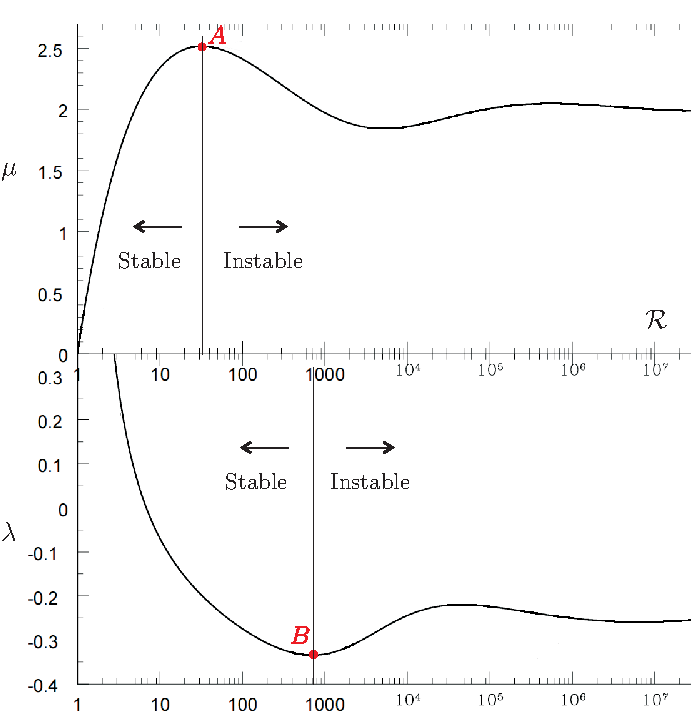
\includegraphics[scale=1.00]{graphe/calorique_stabilite.pdf}
		\caption{Courbes $\lambda(\R)$ et $\mu(\R)$ tirées de l'article \cite{2011MNRAS.414.2728Y}}
		\label{Cal_stab}
	\end{figure}
	Le maximum de l'entropie dans l'ensemble microcanonique ($\delta S=0$ avec $H=\mathrm{cte}$) dans un domaine
	borné correspond à la sphère isotherme en boite. Tous les points de la courbe $\lambda(\R)$ correspondent à
	$\delta S=0$, au point critique $B$ de coordonnées $\R=709$ et $\lambda=-0.335$ nous avons $\frac{d\lambda}{d\R}=0$ et
	$\delta^2 S=0$ (voir \cite{1968MNRAS.138..495L}, \cite{1989ApJS...71..651P} et \cite{1990PhR...188..285P}). Dans
	ces deux derniers articles Padmanabhan (\cite{1989ApJS...71..651P} et \cite{1990PhR...188..285P}) montre que
	tous les points de la courbe $\lambda(\R)$ situés avant $B$ , i.e. $\R < 709$, correspondent à des situations
	telles que $\delta^2 S>0$, ils correspondent à des maxima locaux d'entropie et sont donc des configurations
	stables. Par contre tout ceux situés après le point $B$, i.e. $\R > 709$, sont toujours instables : soit parce
	que $\delta^2 S<0$ dans un premier temps (\cite{1989ApJS...71..651P}), soit pour des raisons dynamiques plus
	compliquées (voir \cite{Katz-Stab} et \cite{1979MNRAS.189..817K}). 
	
	Comme le montre \cite{2002A&A...381..340C}, dans l'ensemble canonique la situation est différente. En lieu et
	place de l'entropie, le potentiel d'étude de la stabilité est l'énergie libre $F=H-TS$. La courbe à étudier est
	maintenant $\mu(\R)$. Elle fait apparaitre deux régions. Tous les points de cette courbe situés avant le point
	$A$ de coordonnées $\R=32,1$ et $\lambda=2,518$, i.e. $\R<32,1$, sont tels que $\delta^2 F>0$ : ils
	correspondent à des sphères isothermes en boite stables. Au delà du point $A$, i.e. $\R>32,1$, le système est
	instable dans l'ensemble canonique.
	
	De manière concrète nous retiendrons que l'étude de la stabilité d'une sphère isotherme en boite est de manière générale contrôlée par son contraste de densité et l'étude des tangentes horizontales ou verticales de sa courbe calorique.   
	\begin{itemize}

		\item Pour une boite isolée aux parois réfléchissantes (situation microcanonique), le point critique de
			stabilité est associé à la tangente verticale la plus à gauche sur la courbe calorique
			$\mu(-\lambda)$ de la figure \ref{Ener}.

		\item Pour une boite dont les parois (conductrices de chaleur...) sont en contact avec un thermostat, le
			point critique de stabilité est associé à la tangente horizontale la plus en haut sur la courbe
			calorique $\mu(-\lambda)$ de la figure \ref{Ener}.

	\end{itemize}
	


%		\section{Numérique}
%			Écrire partie numérique sur milne, ...


\chapter{Le modèle de \textsc{King}\label{King::Chapitre}}
	\minitoc

	Face aux problèmes soulevés par la sphère isotherme singulière et afin de prendre en considération les contingences observationnelles, Ivan
	King proposa en 1966 un nouveau modèle qui consiste à limiter par des arguments physiques et \og à la main\fg l'extension la sphère. Il
	introduit pour cela une énergie maximum, au-delà de laquelle une particule n'est plus liée au système. Cette énergie, qui s'interprète comme
	une énergie de libération, implique une vitesse maximale ainsi qu'un rayon au-delà desquels une particule quitterait le système.

	\section{Équation de \textsc{Poisson}}
		%\subsection{Calcul v2.0}

La fonction de distribution associée à ce modèle de King s'écrit (~voir~\cite{King-1966AJ}~) :
\begin{equation}
	f_K(E) = \begin{cases}
		\rho_0 \(2\pi m\sigma^2\)^{-3/2}\( e^{\frac{E_l-E}{\sigma^2}} - 1\) & \text{si $E < E_l$} \\
		0 & \text{si $E > E_l$}
	\end{cases}
\end{equation}
%\begin{equation}
%	f_K(E) = \left\{\begin{array}{l} \rho_0 \(2\pi m\sigma^2\)^{-3/2}\( e^{\frac{E_l-E}{\sigma^2}} - 1\)\ \mathrm{si}\ E < E_l \\
%		\\
%		0\ \mathrm{si}\ E > E_l
%	\end{array}\right.
%\end{equation}
où la dimension de $\sigma^2$ est celle d'une énergie. Ce paramètre représente la dispersion d'énergie du système.
Le paramètre $\rho_0$ est la densité de masse au centre du système. L'énergie $E_l$  de libération d'une particule s'écrit : $E_l = \frac{p_l^2}{2m} + m\psi(r)$, où $\psi(r)$ est le potentiel gravitationnel de la sphère de King et  $p_l$ l'impulsion de libération fonction de $r$.

La densité de masse s'écrit toujours à partir de la fonction de distribution :
\begin{eqnarray*}
	\rho(r) &=& \int^{p_l}_0\,f_K(E)4\pi p^2dp \\
		&=& \frac{\rho_0}{\(2\pi m\sigma^2\)^{3/2}}\int_0^{p_l}\,\left\{e^{\frac{E_l-E}{\sigma^2}} -1\right\} 4\pi p^2 dp\\
\end{eqnarray*}
L'énergie d'une particule test s'écrit  $E = \frac{p^2}{2m} + m\psi$, on a donc :
\begin{eqnarray*}
	\rho(r) &=& \frac{\rho_0}{\(2\pi m\sigma^2\)^{3/2}} \int_0^{p_l}\,\left\{e^{\frac{E_l - \frac{p^2}{2m} - m\psi}{\sigma^2}} -1\right\} 4\pi p^2 dp\\
		&=& \frac{4\pi \rho_0}{\(2\pi m\sigma^2\)^{3/2}} \(e^{\frac{E_l - m\psi}{\sigma^2}} \int_0^{p_l}\,e^{-\frac{p^2}{2m\sigma^2}} p^2 dp - \int_0^{p_l}\,p^2 dp\)\\
\end{eqnarray*}
Une intégration par partie de la première intégrale permet alors d'écrire
\begin{equation*}
	\rho(r) = \frac{4\pi\rho_0}{\(2\pi m\sigma^2\)^{3/2}} 
	\(e^{\frac{E_l - m\psi}{\sigma^2}} 
	\left[
	-m\sigma^2p_l e^{-\frac{p_l^2}{2m\sigma^2}} + m\sigma^2\int_0^{p_l}\,e^{-\frac{p^2}{2m\sigma^2}} dp
	\right] - \frac{p_l^3}{3}\)
\end{equation*}
En introduisant un nouveau potentiel $\phi(r)$ tel que :
\begin{equation}
	p_l^2 = 2m\(E_l - m\psi(r)\) = 2m\phi(r)
\end{equation}
il vient  maintenant :
\begin{equation*}
	\rho(r) = 
	\rho_0 \(-\sqrt{\frac{4\phi}{\pi\sigma^2}}\(1 + \frac{ 2\phi }{3\sigma^2}\) 
	+ 
	\frac{2e^{\frac{\phi}{\sigma^2}}}{\sqrt{2m\pi\sigma^2}} \int_0^{p_l}\,e^{-\frac{p^2}{2m\sigma^2}} dp\)\\
\end{equation*}
la dernière intégrale s'exprime directement en utilisant la fonction d'erreur
$$\mathrm{erf}(t) = \displaystyle{\frac{2}{\sqrt{\pi}}\int_0^t e^{-u^2}du}$$
la densité du modèle de King s'écrit donc
\begin{eqnarray}
	\rho(r) = \rho_0 \(-\sqrt{\frac{4\phi}{\pi\sigma^2}}\(1 + \frac{ 2\phi }{3\sigma^2}\) + e^{\frac{\phi}{\sigma^2}}\mathrm{erf}\(\sqrt{\phi}/\sigma\)\)
	\label{rho_r}
\end{eqnarray}
L'équation de \textsc{Poisson} pour le potentiel $\phi(r) = E_l - m\psi(r)$ s'écrit donc :
\begin{eqnarray}
	\frac{d}{dr}\(r^2\frac{d\phi}{dr}\) = -4m\pi G r^2\rho_0 \left\{-\sqrt{\frac{4\phi}{\pi\sigma^2}}\(1 + \frac{ 2\phi }{3\sigma^2}\) + e^{\frac{\phi}{\sigma^2}}\mathrm{erf}\(\sqrt{\phi}/\sigma\)\right\} \label{King-Pois}
\end{eqnarray}
Malgré le fait que cette équation n'admette pas de solution explicite, son étude numérique ne pose pas de problème majeur.



	\section{Étude numérique}
		\subsection{Adimensionnement de l'équation de Poisson}
%	Pour adimensionner l'énergie, nous allons nous servir de la quantité $\sigma^2$. % qui à la dimension d'une énergie.
%	Nous introduisons la quantité $r_c$, pour adimensionner les distances, puis
%	nous faisons donc le changement de variable suivant :
	L'adimensionnement des énergies se fait au moyen de $\sigma^2$ et celui des longueurs via $r_c$, en posant :
	\[
			\gamma = \dfrac{\phi}{\sigma^2}
			\quad \mathrm{et}\quad 
			x = \dfrac{r}{r_c}
	\]

	Il vient alors :
	\begin{equation}
		\frac{d}{dx}\(x^2\frac{d\gamma}{dx}\) = -\frac{4m\pi G r_c^2 \rho_0}{\sigma^2}x^2 \left\{-\sqrt{\frac{4\gamma}{\pi}}\(1 + \frac{ 2\gamma }{3}\) + e^{\gamma}\mathrm{erf}\(\sqrt{\gamma}\)\right\}
	\end{equation}

	L'adimensionnement est complet en prenant comme chaque fois dans ce contexte 
	\begin{equation}
		r_c^2 = \frac{\sigma^2}{4m\pi G\rho_0}
		\label{r_c}
	\end{equation}
	L'équation de \textsc{Poisson} a résoudre numériquement s'écrit finalement :
	\begin{equation}
		\frac{d}{dx}\(x^2\frac{d\gamma}{dx}\) = x^2\frac{d^2\gamma}{dx^2} +
		2x\frac{d\gamma}{dx} = -x^2 \left\{-\sqrt{\frac{4\gamma}{\pi}}\(1 + \frac{ 2\gamma }{3}\) + e^{\gamma}\mathrm{erf}\(\sqrt{\gamma}\)\right\}
		\label{Pois-no_dim}
	\end{equation}

\subsection{Conditions aux limites et paramètres du modèle}
	
			Le système étant isolé et à l'équilibre, son centre d'inertie est au repos. Sa symétrie sphérique implique que la résultante des force qui s'applique à une particule test située en $r=0$ s'annule. Cette force est proportionnelle au gradient du potentiel, on a donc
			
			\begin{equation}
				\left.\frac{d\gamma}{dr}\right|_{r=0} = \left.\frac{d}{dr}\(\frac{E_l - m\psi}{\sigma^2}\)\right|_{r=0} = -\frac{m}{\sigma^2}\left.\frac{d\psi}{dr}\right|_{r=0} = 0
			\end{equation}
			En l'absence de vitesse, l'énergie minimale est atteinte pour la plus petite valeur de $m\psi(r)$, soit $m\psi(0)$.

			La quantité $\phi(r)=E_l-m\psi(r)$ représente la quantité d'énergie qu'il faut fournir à une particule située à la distance $r$
			du centre du système afin qu'elle sorte du système. 
			Il est clair que le potentiel $\psi(r)$ est une fonction partout négative ou nulle, ainsi
			$\phi(r)$ est à l'inverse positive ou nulle. Au centre, cette quantité vaudra :
			$$\phi(0)=E_l-m\psi(0)$$

			Il est donc commode d'introduire la quantité initiale adimensionnée :
			\begin{equation}
				W_0 = \gamma(0)=\frac{E_l - m\psi(0)}{\sigma^2} > 0
				\label{W_0}
			\end{equation}

			Nous éviterons de la prendre nulle, car, dans ce cas, le système contient au
			plus une étoile !

	Le choix de $\gamma(0)=W_0$ et le fait que la dérivée de $\gamma$ en $r=0$ soit nulle permettent la résolution numérique de l'équation (\ref{Pois-no_dim}). Cette résolution permet d'obtenir le rayon $R$ de la sphère de King, premier zéro de la fonction $\phi(r)$. La vitesse d'une particule test située en $r=R$ est la vitesse de libération du système, en introduisant $X=\frac{R}{r_c}$ on a bien
		\begin{equation}
			 E_l = m\psi(X) \;\Leftrightarrow\; \gamma(X) = 0
		\end{equation}

	Le paramètre $W_0$ fixe donc toutes les caractéristiques nécessaires à la résolution numérique du modèle de King. Le rayon de la sphère de King est une fonction croissante de $W_0$. Comme on peut le voir sur la définition (\ref{W_0}), une même valeur de $W_0$ peut correspondre à des systèmes possédant des caractéristiques physiques différentes caractérisées par une profondeur du puits de potentiel $\psi(0)$, une dispersion de vitesse $\sigma^2$ ou une énergie de libération différente. Ces différences ne concernent que le système une fois redimensionné. 

\subsection{Résolution numérique}
	L'algorithme que nous utiliserons pour résoudre cette équation est un \textsc{Runge-Kutta}
	d'ordre $4$ (~RK4~). Nous devons écrire l'équation différentielle comme un système d'ordre 1, ce que nous faisons en posant $u = \frac{d\gamma}{dx}$ :
	\begin{equation}
		\left\{\begin{array}{l}
			u = \x{\gamma}\\
			\\
			\x{u} = -\left\{-\sqrt{\frac{4\gamma}{\pi}}\(1 + \frac{ 2\gamma }{3}\) + e^{\gamma}\mathrm{erf}\(\sqrt{\gamma}\)\right\} - 2\frac{u}{x}
		\end{array}\right.\label{sys2dking}
	\end{equation}

%	Euh .... Outre un problème évident de division par zéro en $x=0$, qui peut-être résolu à
%	l'aide d'un développement limité du potentiel au centre, lors de l'intégration, la solution
%	pour le potentiel est positive !!! \textcolor{red}{$\Rightarrow$ Normal, j'ai
%	oublié de repasser au potentiel !!! Je trace $\gamma$, et non $\psi$, qui est forcément
%	positif !!!}
	Un terme en $1/x$ est apparu, l'équation semble donc singulière en $0$. Un rapide
	développement limité de la fonction $\gamma$ autour de $0$ nous apprend qu'il n'en est rien, il n'y a
	pas de divergence. Un rapide calcul montre que toutes les dérivées d'ordre impair de $\gamma(x)$ s'annulent en $x=0$, et que 
	$$
	\gamma(0) = W_0\, ,\;\; \gamma''(0) = -\frac{\rho(W_0)}{3\rho_0}\; \mathrm{et}\; \gamma^{(4)}(0) = \frac{2\rho(W_0)}{5\rho_0}\left\{\sqrt{\frac{W_0}{\pi}} -
			\frac{e^{W_0}\mathrm{erf}(\sqrt{W_0})}{2}\right\} 
	$$
On peut donc écrire directement un développement de Taylor de $\gamma(x)$ à l'ordre 5 en $x=0$. 
	La résolution des équations nous permet alors d'avoir les graphiques de la
	figure~\ref{King_Modele-test} (~les graphes sont adimensionnés~).% mais pas normalisé~).
%	\paragraph{Problème : Résolu :}
%	Tant que la variable $x$ est proche de $0$, j'utilise les développements limités, puis passé
%	un certain seuil, je réutilise l'équation différentielle. Le résultat obtenu est la figure~\ref{King_Modele-err}
%	au lieu de la figure~\ref{King_Modele} (~figure pour laquelle je démarre à $x=1.10^{-6}$ au
%	lieu de $x=0$~). Il semblerait que mon algorithme de RK4 à pas variable ait du mal à suivre,
%	en plus d'avoir, apparemment, une erreur d'adimensionnement/normalisation.
%	\subparagraph{Solution pour le RK4 ne suivant pas :} J'utilisais le développement de $\gamma(x)$ pour calculer la pente
%	et celui de $\x{\gamma(x)}$ pour calculer la dérivée seconde.

%	\textcolor{red}{RAAAAAAHHHHHHHHH !!!!!!!!!! Plein d'erreur de signe dans les calculs et le
%	programme !!!!!!!!!!! Faut tout revérifier !!!!!!!!!!!!!!!!!!!}

%	\begin{figure}[ht!]
%			\begin{minipage}[b]{0.40\linewidth}
%				\centering 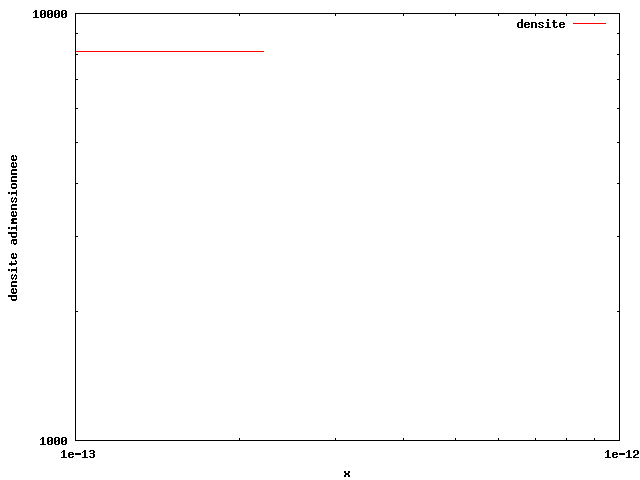
\includegraphics[scale=0.40]{graphe/erreur_king.png}
%			\end{minipage}\hfill
%			\begin{minipage}[b]{0.48\linewidth}
%				\centering 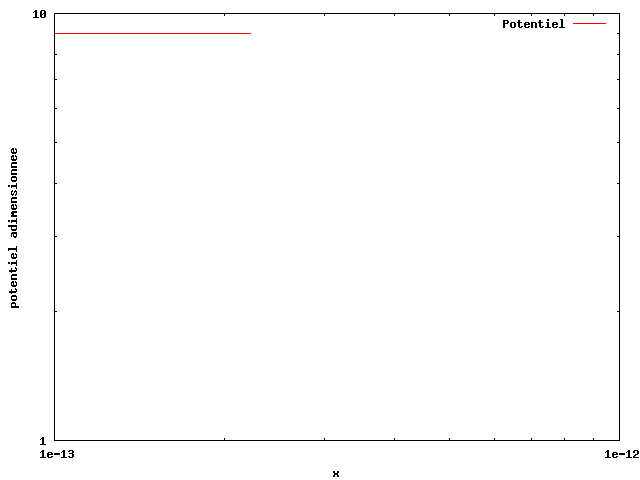
\includegraphics[scale=0.40]{graphe/erreur-pot_king.png}
%			\end{minipage}
%			\caption{Densité et potentiel d'un modèle de \textsc{King} pour les
%			conditions initiales (~au centre~) : $\gamma(0) = \frac{E_l -
%			m\psi(0)}{\sigma^2} = 9$}
%			\label{King_Modele-err}
%	\end{figure}
%	\begin{figure}[ht!]
%			\begin{minipage}[b]{0.40\linewidth}
%				\centering \includegraphics[scale=0.60]{graphe/densite_king.pdf}
%			\end{minipage}\hfill
%			\begin{minipage}[b]{0.48\linewidth}
%				\centering \includegraphics[scale=0.60]{graphe/potentiel_king.pdf}
%			\end{minipage}
%			\caption{Densité et potentiel d'un modèle de \textsc{King} pour les
%			conditions initiales (~au centre~) : $\gamma(0) = \frac{E_l - m\psi(0)}{\sigma^2} = 3$, $\x{\gamma}(0) = 0$}
%			\label{King_Modele}
%	\end{figure}

	\begin{figure}[ht!]
			\begin{minipage}[b]{0.40\linewidth}
				\centering \includegraphics[scale=0.60]{graphe/densite_pluri-king.pdf}
			\end{minipage}\hfill
			\begin{minipage}[b]{0.48\linewidth}
				\centering \includegraphics[scale=0.60]{graphe/densite_pluri_limite-king.pdf}
			\end{minipage}
			\caption{CETTE LEGENDE N4EST PAS SUFFISANTE ! IL FAUT INDIQUER CE QU4EST CETTE FONCTION $\rho(x)$ PARCE CE QUE L4ON CALCULE C4EST $\gamma(x)$.
			Densité d'un modèle de \textsc{King} pour les conditions initiales
			(~au centre~) : $\gamma(0) = 1$ (~courbe rouge~), $5$ (~courbe verte~), $9$ (~courbe bleu~), $14$ (~courbe violette~), $\x{\gamma}(0) = 0$}
			\label{King_Modele-test}
	\end{figure}

	%La figure~\ref{King_Modele-test} montre l'aspect de la densité d'un modèle de \textsc{King} en fonction de $W_0$ et nous indique aussi que ce modèle posséde une structure cœur-halo
	%(~une partie quasiment constante suivi d'une décroissance auto-similaire de pente $\alpha$~).
	%Plus $\phi$ est grand, plus le cœur est dense (~le graphe de droite trace $\rho(x)/\rho(0)$~). Nous pouvons aussi observer que la pente n'est pas la même :
	%elle diminue (~la courbe tend plus vite vers $0$~). Ce constat nous amène à nous poser une question : existe-t-il un
	%lien entre la pente et le rayon du cœur ?
	
	La résolution numérique du système (\ref{sys2dking}) permet d'obtenir la fonction $\gamma(x)$ pour chaque donnée initiale $W_0$. De cette fonction on déduit la densité volumique de masse du système $\rho(x)$ par la relation XXXXXXXXXX. Une sphère de King adimensionnée est donc entièrement définie par le paramètre $W_0$. En échelle logarithmique, sa densité normalisée est très bien approchée sur plus de 5 décades par deux segments de droites : l'un horizontal décrit le c\oe ur de la sphère de densité quasiment constante, l'autre de pente $-\alpha$ décrit un halo autosimilaire entourant le c\oe ur. L'intersection des droites portant ces deux segments est une bonne approximation de ce que l'on pourrait appeler le rayon du c\oe ur de la sphère de King considérée.
		
	Pour les petites valeurs de $W_0$, typiquement $W_0\leq 5$, la sphère de King est essentiellement constituée d'un très large c\oe ur de densité quasiment constante. Par contre dès que  $W_0\geq 15$, le c\oe ur ne renferme plus qu'une faible proportion de la masse du système et la sphère de King est essentiellement constituée d'un halo autosimilaire dont la densité est comparable à celle d'une sphère isotherme. Cette comparaison n'est valide que jusqu’à un certain rayon où la densité de la sphère de King chute violemment  à cause de la troncature introduite par l'énergie de libération.
	Une étude plus fine menée pendant notre stage de M2 montre que les halos des sphères de King sont associés à des profils autosimilaires de pente étagées entre $-5$  et $-2$ lorsque $W_0$ varie de $5$ à $15$.
	
	\begin{figure}[hbt!]
%		\centering \includegraphics[scale=1.00]{../Resol_King/img-king/pente-w0.pdf} %{graphe/evo-coeff_ci.pdf}
		\centering \includegraphics[scale=1.00]{graphe/pente-w0.pdf}%{img-king/pente-w0.pdf} %{graphe/evo-coeff_ci.pdf}
		\caption{Évolution de la pente du halo de la sphère de King en fonction de $W_0$}
		\label{coeff_evo}
	\end{figure}
	
	Une sphère de King définie par une grande valeur de $W_0$ est donc très proche d'une sphère isotherme, sa température est donc vraisemblablement indépendante de la distance au centre. Il est intéressant de préciser cette idée de façon plus quantitative. C'est l'objet de la prochaine section.
	
	\FloatBarrier


%%		\newpage
	%\section[Relation entre les paramètres]{Relation entre les différents paramètres d'un modèle de \textsc{King}\label{pente-coeff_sec}}
		%	Nous nous intéressons maintenant à l'existence d'un lien entre le rayon du cœur et la pente
du halo. Il n'y a apparemment aucun moyen de faire ça analytiquement (~en tout cas, je n'ai pas encore trouvé~).
Par contre, lorsque je traçais des graphes, obtenu avec le code abordé ci-dessus,
j'ai remarqué une forte dépendance\footnote{logique~!?!} entre la pente, en $\log-\log$, et $W_0$
(~voir graphe de droite de la figure~\ref{King_Modele-test}~). De même pour le rayon à $10\%$
de l'objet étudié. L'idée que j'ai utilisé pour faire le lien entre les deux quantités a été de
regarder leur comportement en fonction des conditions initiales puis de combiner ensuite les 2
comportements pour obtenir une relation empirique entre ces deux paramètres. %courbe les reliant.

\subsection{Calcul des pentes pour différentes conditions initiales\label{pente-critére}}

	Pour obtenir les pentes, nous traçons dans un diagramme $\log-\log$ la densité, puis, à l'aide
du logiciel \textsc{GNUPlot}\footnote{\url{http://www.gnuplot.info/}} nous ajustons une équation du type $a x+b$ à la partie linéaire de la
courbe, le coefficient $a$ représentant la pente.

	Le problème avec cette méthode, c'est que, pour certaines conditions initiales, il n'y a
presque pas de halo : la densité d'étoile chute brutalement (~voir figure~\ref{ci-pente_1}
page~\pageref{ci-pente_1} en annexe~). Les valeurs des pentes pour des systèmes ayant une énergie de
libération et une énergie minimale très proche, ou une grande dispersion d'énergie, sont donc assez
peu fiables. Cette brusque pente vient de la faible quantité d'énergie à fournir pour faire
s'échapper une ou plusieurs particules du système.

	Le traitement a ensuite été automatisé en considérant que le halo correspond à la zone :
	\begin{align}
		10^{-4} < \dfrac{\rho(r)}{\rho(0)} < 0.1 \label{pente::critere}
	\end{align}

	Pour obtenir les points rouge de la figure~\ref{coeff_evo}, nous avons fait varier $\gamma(0) = W_0 = 1$ à $W_0 = 21$.
	La courbe verte est obtenu en ajustant aux points rouge, et en respectant le critère~\ref{pente::critere}, une équation du type $a e^{b x} + c$. %$a x^2 + b x + c$.
	Les coefficients obtenus sont donnés sur la courbe~\ref{coeff_evo}.
%	\begin{table}[hbt!]
%		\begin{center}
%			\begin{tabular}{|c|c|c|}
%				\hline
%				Coefficient & Valeur & Erreur \\
%				\hline
%				\hline
%				$a$       &         -10.0698      &  $\pm 0.2423$       (~$2.406\%$~) \\
%				\hline
%				$b$       &         0.220152      &  $\pm 0.01075$      (~$4.883\%$~) \\
%				\hline
%				$c$       &         -1.63409      &  $\pm 0.09393$      (~$5.748\%$~) \\
%				$a$       &        $-0.0157022$   &   $\pm 0.002226$ (~$14.18\%$~) \\
%				$b$       &        $0.443128$     &   $\pm 0.03663$  (~$8.266\%$~) \\
%				$c$       &        $-5.33431$     &   $\pm 0.1274$   (~$2.388\%$~) \\
%				\hline
%			\end{tabular}
%		\end{center}
%		\caption{Valeur des coefficients donnée par l'ajustement pour les pentes}
%		\label{pente-fit}
%	\end{table}
	\begin{figure}[hbt!]
%		\centering \includegraphics[scale=1.00]{../Resol_King/img-king/pente-w0.pdf} %{graphe/evo-coeff_ci.pdf}
		\centering \includegraphics[scale=1.00]{graphe/pente-w0.pdf}%{img-king/pente-w0.pdf} %{graphe/evo-coeff_ci.pdf}
		\caption{Évolution des pentes pour différentes conditions initiales}
		\label{coeff_evo}
	\end{figure}

	Il est réconfortant de remarquer sur cette courbe la présence d'une asymptote horizontale autour de $-2$ correspondant à la pente d'une sphère isotherme singulière.
	En effet, pour $W_0 \to \infty$ le modèle de \textsc{King} se rapproche d'une sphère isotherme de rayon infini dont le halo est très proche de celui d'une SIS.
%	\FloatBarrier

\subsection{Calcul du rayon à $10\%$ pour différentes conditions initiales\label{r_10}}

	L'un des paramètres libres les plus utilisés du modèle de \textsc{King} est le rayon du cœur (formule~\ref{r_c}, page~\pageref{r_c}~).
%	Il serait ainsi intéressant de prendre cette valeur et de la tracer en fonction de la condition initiale $W_0$,
%	ce qui nous permettrait ainsi de la relier à la pente.
	Il est donc intéressant de relier les paramètres $r_c$ et $W_0$. Ainsi, en utilisant la relation que nous avons déterminé entre $W_0$ et la pente $\alpha$ du halo, nous obtiendrons une relation entre $r_c$ et $\alpha$

	Mais deux problèmes se posent :
	\begin{enumerate}
		\item de la même manière que dans le paragraphe précédent, la détermination de $r_c$ a un problème : quand
	$W_0$ devient trop grand, le système se \og~dilue~\fg, c'est-à-dire que la différence entre
	cœur et halo est de moins en moins évidente, comme sur la figure~\ref{w_0-5_10}
	page~\pageref{w_0-5_10} (~nous sommes dans le cas d'un amas effondré~),
		\item le programme de résolution qui nous permet d'avoir ces courbes est adimensionné par rapport à ce rayon, rendant ainsi très difficile
			le redimensionnement des résultats et leur comparaison avec les données observationnelles.
	\end{enumerate}

	Pour palier à ce dernier problème, il est possible de prendre, plutôt que le rayon du cœur, le rayon à $10\%$.
%	Le rayon à $10\%$ est le rayon à partir duquel $10\%$ de la masse totale de l'amas se trouve à l'intérieur.
	Il est défini comme :
	\begin{quote}
		Le rayon à $10\%$ du système est atteint lorsque, du centre vers le bord du
		système, la densité a diminué de $10\%$ :
		\begin{align}
			\frac{\rho(x_{10})}{\rho(0)} = 0.1
		\end{align}
	\end{quote}

%	Le rayon à $10\%$ est plus délicat à obtenir.
%	Pour obtenir la figure~\ref{coeur_evo}, nous avons considéré que le rayon à $10\%$ correspondait à la distance pour laquelle la densité
%	ne pouvait plus être considérée comme constante : nous avons placé, à la main, la valeur du
%	rayon au moment où la pente devenait nette\footnote{cette contrainte dépend des gens et n'est donc
%	pas très adapté à ce que nous faisons}.

	Une fois ces valeurs de rayon mesurées, nous avons tracé la courbe rouge de la
	figure~\ref{coeur_evo2} que nous avons ajustée avec la fonction $a e^{b x} + c$ et avons
	obtenu les coefficients indiqués sur la courbe.

%	\begin{table}[hbt!]
%		\begin{center}
%			\begin{tabular}{|c|c|c|}
%				\hline
%				Coefficient & Valeur & Erreur \\
%				\hline
%				\hline
%				$d$       &       $1.86332$      &   $\pm 0.04078$ 	(~$2.189\%$~)\\
%				\hline
%				$e$       &       $-0.635746$    &   $\pm 0.01585$    	(~$2.494\%$~)\\
%				\hline
%				$f$       &       $0.0049355$    &   $\pm 0.003953$     (~$80.1\%$~)\\
%				\hline
%			\end{tabular}
%		\end{center}
%		\caption{Valeur des coefficients donnée par l'ajustement pour les rayons à $10\%$}
%		\label{coeur-fit}
%	\end{table}
%	\begin{figure}[hbt!]
%		\centering \includegraphics[scale=1.00]{graphe/evo-coeur_ci.pdf}
%		\caption{Évolution du rayon à $10\%$ calculé à la main pour différents $W_0$}
%		\label{coeur_evo}
%	\end{figure}

%	\textcolor{red}{\underline{Attention :}} il peut être intéressant de refaire ces courbes en
%	incluant le calcul du rayon à $10\%$ directement dans le code (~selon la définition choisi~).

%	Le calcul a été refait en sortant le rayon à $10\%$ directement du code résolvant les
%	équations. De cette manière, la courbe reste sensiblement la même, et les coefficients ont par contre
%	bien changé, comme nous pouvons le voir sur la courbe~\ref{coeur_evo2}.
	\begin{figure}[hbt!]
		\centering \includegraphics[scale=1.00]{graphe/evo-coeur_ci2.pdf}
		\caption{Évolution du rayon à $10\%$ calculé lors de la résolution numérique pour différents $W_0$}
		\label{coeur_evo2}
	\end{figure}
%	\begin{table}[hbt!]
%		\begin{center}
%			\begin{tabular}{|c|c|c|}
%				\hline
%				Coefficient & Valeur & Erreur \\
%				\hline
%				\hline
%				$d$        &       $7.36877$      &   $\pm 0.2352$       (~$3.191\%$~)\\
%				\hline
%				$e$        &       $-0.633846$    &   $\pm 0.02309$      (~$3.642\%$~)\\
%				\hline
%				$f$        &       $0.0419222$    &   $\pm 0.02291$      (~$54.66\%$~)\\
%				\hline
%			\end{tabular}
%		\end{center}
%		\caption{Valeur des coefficients donnée par l'ajustement pour les rayons à $10\%$
%		(~v2.0~)}
%		\label{coeur-fit2}
%	\end{table}
	\FloatBarrier

\subsection{Lien entre les deux\label{ssec::LinkBetween}}

	Maintenant que nous avons la dépendance des rayons à $10\%$ et des pentes en fonction de la
	condition initiale $W_0$, nous pouvons regarder comment varie la pente en fonction de la
	taille de l'amas. Sur la figure~\ref{coeff-coeur2}, nous avons tracé en vert les données, et
	en rouge la courbe formée par nos deux expressions obtenues par ajustement (~les coefficients
	utilisés sont les mêmes que ceux donnés sur les figures~\ref{coeff_evo} et~\ref{coeur_evo2}~).
%	\begin{figure}[hbt!]
%		\centering \includegraphics[scale=1.00]{graphe/evo-coeff_coeur.pdf}
%		\caption{Évolution de la pente calculé à la main en fonction du rayon à $10\%$}
%		\label{coeff-coeur}
%	\end{figure}

	En supposant que nos ajustements sont valables pour toutes les valeurs possibles de $W_0$,
	nous pouvons tenter d'obtenir une expression analytique reliant nos deux quantités. En
	partant de :
	\begin{align}
		\left\{\begin{array}{l}
			f(W_0) = \alpha = a e^{b W_0} + c \\ %a W_0^2 + b W_0 + c \\
			g(W_0) = x_{10\%} = d e^{e W_0} + f
		\end{array}\right.
	\end{align}
	Et en les combinant :
	\begin{align}
		\Rightarrow e^{e W_0} &= \frac{x_{10\%} - f}{d} \notag\\
				W_0   &= \frac{1}{e}\ln\(\frac{x_{10\%} - f}{d}\) \\
		\Rightarrow \alpha &= a \exp\(\frac{1}{e}\ln\(\frac{x_{10\%} - f}{d}\)\) + c %\frac{a}{e^2}\ln^2\(\frac{x_{10\%} - f}{d}\) +
					%\frac{b}{e}\ln\(\frac{x_{10\%} - f}{d}\) + c \notag \\
%		\intertext{Nous obtenons :}
%		\beta &= a e^{1/e} %\frac{1}{e}\ln\(\frac{x_{10\%} - f}{d}\)\(\frac{a}{e}\ln\(\frac{x_{10\%} - f}{d}\) + b\) + c
	\end{align}

	Cette expression s'ajuste \og~bien~\fg~à la courbe, mais \textsc{GNUPlot} donne des erreurs
	assez élevées.
%	\begin{table}[hbt!]
%		\begin{center}
%			\begin{tabular}{|c|c|c|}
%				\hline
%				Coefficient & Valeur & Erreur \\
%				\hline
%				\hline
%				$q=a/e^2$       &      $-0.0394991$   &   $\pm 0.02115$ (~$53.55\%$~)\\
%				\hline
%				$s=1/d$         &      $0.524033$     &   $\pm 4.538$   (~$865.9\%$~)\\
%				\hline
%				$j=f/d$         &      $0.00254127$   &   $\pm 0.02122$ (~$835.2\%$~)\\
%				\hline
%				$k=b/e$         &      $-0.688944$    &   $\pm 0.8111$  (~$117.7\%$~)\\
%				\hline
%				$l=c$           &      $-5.3267$      &   $\pm 6.127$   (~$115\%$~)\\
%				\hline
%			\end{tabular}
%		\end{center}
%		\caption{Valeur des coefficients donnée par l'ajustement pour les pentes en
%		fonctions des rayons à $10\%$}
%		\label{param-fit}
%	\end{table}
%	Les corrections dans la détermination du rayon à $10\%$ ont amélioré l'ajustement de cette courbe, en plus d'avoir changé l'échelle des $x$. Les changements sont
%	donnés sur la figure~\ref{coeff-coeur2}.
%	\begin{table}[hbt!]
%		\begin{center}
%			\begin{tabular}{|c|c|c|}
%				\hline
%				Coefficient & Valeur & Erreur \\
%				\hline
%				\hline
%				$q$       &       $-0.0526849$    &  $\pm 0.02245$      (~$42.6\%$~)\\
%				\hline
%				$s$       &       $0.211927$      &  $\pm 0.4648$       (~$219.3\%$~)\\
%				\hline
%				$j$       &       $0.0081136$     &  $\pm 0.02144$      (~$264.2\%$~)\\
%				\hline
%				$k$       &       $-0.716362$     &  $\pm 0.1606$       (~$22.42\%$~)\\
%				\hline
%				$l$       &       $-5.01452$      &  $\pm 1.478$        (~$29.47\%$~)\\
%				\hline
%			\end{tabular}
%		\end{center}
%		\caption{Valeur des coefficients donnée par l'ajustement pour les pentes en
%		fonctions des rayons à $10\%$ (~v2.0~)}
%		\label{param-fit2}
%	\end{table}
	\begin{figure}[hbt!]
		\centering \includegraphics[scale=1.00]{graphe/evo-coeff_coeur3.pdf}
		\caption{Évolution de la pente en fonction du rayon à $10\%$}
		\label{coeff-coeur2}
	\end{figure}

%	Ensuite, il est intéressant de comparer les données observationnelle à notre travail. Le problème auquel auquel nous avons fait face est
%	que nous avons adimensionné le problème par rapport au rayon de cœur, qu'il n'est donc pas possible d'obtenir par la résolution numérique.
%	Ce travail n'est donc pas utilisable directement pour une comparaison avec les observations. Par contre, le rayon de cœur est mesurable, comme indiqué dans~\cite{Djo-rc}.
	\FloatBarrier

\subsection{Paramètre de concentration : $c$}
	Le dernier paramètre d'un modèle de \textsc{King} sur lequel nous pouvons jouer est le paramètre de concentration $c$.
	Dans le modèle de King, la concentration s'écrit :
	\begin{align}
		c = \log_{10}\(\frac{R}{r_c}\)
	\end{align}
	avec $R$ la taille du système (~tel que $\rho(R) = 0$~) et $r_c$ le rayon de cœur. Ce paramètre est infini pour la sphère isotherme singulière, comme $W_0$.
	Notons que dans le cas de la SIS $W_0$, $R$ et $c$ sont infini.

	Ce paramètre permet aussi de fixer l'état du système. Trouver une fonction ou une équation permettant de faire le lien entre la concentration et la condition
	initiale $W_0$ nous permettrait de trouver le modèle de King correspondant à un amas (~les paramètres $c$, $r_c$ et $\sigma^2$ le représentant~). Nous avons donc inclus
	dans la résolution des équations un calcul de ce paramètre de concentration. Nous avons ainsi pu obtenir la courbe~\ref{concentre}
	\begin{figure}[hbt!]
		\centering \includegraphics[scale=1.00]{graphe/concentration-king.pdf}
		\caption{Évolution de la concentration avec la condition initiale $W_0$}
		\label{concentre}
	\end{figure}

	Le paramètre de concentration est mesurable pour chaque amas (~en tout cas, c'est un des paramètres du catalogue de \textsc{Harris}~\cite{Harris}~).
	Mais le fait que la courbe ne soit pas bijective nous impose plusieurs modèles pour un seul paramètre de concentration.
	\FloatBarrier


	\section{Température d'un modèle de \King \label{sec::temp}}
		L'une des premières questions que l'on peut se poser, par rapport au modèle précèdent~: le modèle de \King est il isotherme~?

%Dans un premier temps, nous rappelons les expressions des fonctions de distribution et densité pour ce modèle~:
%\begin{align}
%	f_K(E) &= \begin{cases}
%		\rho_0 \(2\pi m\sigma^2\)^{-3/2}\( e^{\frac{E_l-E}{\sigma^2}} - 1\) & \text{si $E < E_l$} \\
%		0 & \text{si $E > E_l$}
%	\end{cases} \\
%	\rho(r) &= \rho_0 \(-\sqrt{\frac{4\phi}{\pi\sigma^2}}\(1 + \frac{ 2\phi }{3\sigma^2}\) + e^{\frac{\phi}{\sigma^2}}\mathrm{erf}\(\sqrt{\phi}/\sigma\)\)
%\end{align}

La température est définit comme étant proportionnelle à la dispersion de vitesse tel que~:
\begin{align}
	T(r) &\propto \dfrac{\int p^2 f_K(E) \vdp}{m^2 \int f_K(E) \vdp} & v^2 = \frac{p^2}{m^2}
\end{align}

\subsection{Évolution de la température avec le rayon}

Le numérateur s'écrit~:
\begin{align}
	\int_0^{p_l} \dfrac{p^2}{m^2} f_K\(E\) \mathrm{d}\vec{p} &= \int_0^{p_l} \dfrac{p^2}{m^2} \rho_0 \(2\pi m\sigma^2\)^{-3/2}\( e^{\frac{E_l-E}{\sigma^2}} - 1\) 4\pi p^2 \ddp \notag \\
	    &= \dfrac{4\pi\rho_0}{\(2\pi m\sigma^2\)^{3/2}}\(\int_0^{p_l} \frac{p^4}{m^2} e^{\frac{E_l-E}{\sigma^2}}\ddp -
	    \int_0^{p_l} \frac{p^4}{m^2}\ddp \) \notag
\intertext{En utilisant $E = \dfrac{p^2}{2m} + m\psi$, et à l'aide d'intégration par partie, il est possible de simplifier plusieurs étapes de l'intégration~:}
	    &= \frac{4\pi\rho_0}{m^2\(2\pi m\sigma^2\)^{3/2}}
	    	\(
			e^{\frac{E_l - m\psi}{\sigma^2}}
			\left[
				3m\sigma^2\int_0^{p_l} p^2 e^{-\frac{p^2}{2m\sigma^2}}\ddp
				- m\sigma^2 p_l^3 e^{-\frac{p_l^2}{2m\sigma^2}}
			\right]
			- \dfrac{p_l^5}{5}
	    	\) \notag \\
	    &= \frac{4\pi\rho_0}{m^2\(2\pi m\sigma^2\)^{3/2}}
		\(
			e^{\frac{E_l - m\psi}{\sigma^2}}
	    		\left[
				  3\(m\sigma^2\)^2 \int_0^{p_l} e^{-\frac{p^2}{2m\sigma^2}} \ddp
				- 3\(m\sigma^2\)^2p_le^{-\frac{p_l^2}{2m\sigma^2}}
			\right. \right. \notag \\
				&\qquad \left.\vphantom{ e^{-\frac{p_l^2}{2m\sigma^2}}}\left.\vphantom{e^{-\frac{p_l^2}{2m\sigma^2}}}
				- m\sigma^2 p_l^3 e^{-\frac{p_l^2}{2m\sigma^2}}
			\right]
	    		- \dfrac{p_l^5}{5}
		\) \notag \\
	    &= \frac{4\pi\rho_0}{m^2\(2\pi m\sigma^2\)^{3/2}}
		\(
			e^{\frac{E_l - m\psi}{\sigma^2}}\(m\sigma^2\)^2
	    		\left[
				  3 \int_0^{p_l} e^{-\frac{p^2}{2m\sigma^2}} \ddp
				- 3p_le^{-\frac{p_l^2}{2m\sigma^2}}
				\(1 + \dfrac{p_l^2}{3m\sigma^2}\)
			\right] \right. \notag \\
	    &\qquad \left.\vphantom{ e^{-\frac{p_l^2}{2m\sigma^2}}}
	    		- \dfrac{p_l^5}{5}
		\) \notag \\
	    &= \frac{4\pi\rho_0}{m^2\(2\pi m\sigma^2\)^{3/2}}
		\(
			e^{\frac{E_l - m\psi}{\sigma^2}}\(m\sigma^2\)^2
	    		\left[
				3 \dfrac{\sqrt{\pi}}{2}\sqrt{2m\sigma^2}\erf\(\dfrac{p_l}{\sqrt{2m\sigma^2}}\)
				- 3p_le^{-\frac{p_l^2}{2m\sigma^2}}
				\(1 + \dfrac{p_l^2}{3m\sigma^2}\)
			\right] \right. \notag \\
	    &\qquad \left.\vphantom{ e^{-\frac{p_l^2}{2m\sigma^2}}}
	    		- \dfrac{p_l^5}{5}
		\) \notag \\
%	    &= \frac{12\pi\rho_0 \sigma^4}{\(2\pi m\sigma^2\)^{3/2}} e^{\frac{E_l - m\psi\(r\)}{\sigma^2}} h\(p_l\)\dr
\intertext{avec $p_l = \sqrt{2m\(E_l - m\psi(r)\)} = \sqrt{2m\phi(r)}$~:}
	    &= \frac{4\pi\rho_0}{m^2\(2\pi m\sigma^2\)^{3/2}}
		\(
			e^{\frac{\phi}{\sigma^2}}\(m\sigma^2\)^2
	    		\left[
				3\dfrac{\sqrt{\pi}}{2} \sqrt{2m\sigma^2}\erf\(\dfrac{\sqrt{2m\phi(r)}}{\sqrt{2m\sigma^2}}\)
			\right. \right. \notag \\
	    &\qquad \left.\vphantom{ e^{-\frac{2m\phi(r)}{2m\sigma^2}}}\left.\vphantom{ e^{-\frac{2m\phi(r)}{2m\sigma^2}}}
			        - 3\sqrt{2m\phi(r)}e^{-\frac{2m\phi(r)}{2m\sigma^2}}
				\(1 + \dfrac{2m\phi(r)}{3m\sigma^2}\)
			\right]
			- \dfrac{\(2m\phi(r)\)^{5/2}}{5}
		\) \notag \\
	    &= \frac{4\pi\rho_0}{m^2\(2\pi m\sigma^2\)^{3/2}}
		\(
			\dfrac{3}{2} \(m\sigma^2\)^2\sqrt{2m\pi\sigma^2}
	    		\left[
				e^{\frac{\phi}{\sigma^2}}\erf\(\sqrt{\dfrac{\phi(r)}{\sigma^2}}\)
			\right. \right. \notag \\
	    &\qquad \left.\vphantom{\(\sqrt{\dfrac{\phi(r)}{\sigma^2}}\) }\left.\vphantom{\(\sqrt{\dfrac{\phi(r)}{\sigma^2}}\)}
				- \sqrt{\dfrac{4\phi(r)}{ \pi\sigma^2}}
				\(1 + \dfrac{2\phi(r)}{3\sigma^2}\)
			\right]
			- \dfrac{\(2m\phi(r)\)^{5/2}}{5}
		\) \notag
\end{align}

La température va alors s'écrire~:
\begin{align}
	T(r) &\propto \frac{4\pi\rho_0}{m^2\(2\pi m\sigma^2\)^{3/2}}
		\(
		\dfrac{
			\dfrac{3}{2} \(m\sigma^2\)^2\sqrt{2m\pi\sigma^2}
	    		\left[
				e^{\frac{\phi}{\sigma^2}}\erf\(\sqrt{\dfrac{\phi(r)}{\sigma^2}}\)
				- \sqrt{\dfrac{4\phi(r)}{ \pi\sigma^2}}
				\(1 + \dfrac{2\phi(r)}{3\sigma^2}\)
			\right]
		}
		{
			\rho_0 \(-\sqrt{\frac{4\phi}{\pi\sigma^2}}\(1 + \frac{ 2\phi }{3\sigma^2}\) + e^{\frac{\phi}{\sigma^2}}\mathrm{erf}\(\sqrt{\phi}/\sigma\)\)
		}
			\right. \notag \\
	    &\qquad \left.
		- \dfrac{
			\(2m\phi(r)\)^{5/2}
		}
		{
			5 \rho_0 \(-\sqrt{\frac{4\phi(r)}{\pi\sigma^2}}\(1 + \frac{ 2\phi(r) }{3\sigma^2}\) + e^{\frac{\phi(r)}{\sigma^2}}\mathrm{erf}\(\sqrt{\phi(r)}/\sigma\)\)
		}
		\) \notag \\
	&\propto \frac{4\pi}{m^2\(2\pi m\sigma^2\)^{3/2}} \(m\sigma^2\)^2
		\(
			\dfrac{3}{2}\sqrt{2m\pi\sigma^2}
		- \dfrac{
			\(2m\phi(r)\)^{5/2} \(m\sigma^2\)^{-2}
		}
		{
			5 \(-\sqrt{\frac{4\phi(r)}{\pi\sigma^2}}\(1 + \frac{ 2\phi(r) }{3\sigma^2}\) + e^{\frac{\phi(r)}{\sigma^2}}\mathrm{erf}\(\sqrt{\phi(r)}/\sigma\)\)
		}
		\) \notag \\
	&\propto \sqrt{\dfrac{2\sigma^2}{m^3\pi}}							%\frac{4\pi}{m^2\(2\pi m\sigma^2\)^{3/2}} \(m\sigma^2\)^2
		\(
			\dfrac{3}{2}\sqrt{2m\pi\sigma^2}
		- \dfrac{
			\(2m\phi(r)\)^{5/2} \(m\sigma^2\)^{-2}
		}
		{
			5 \(-\sqrt{\frac{4\phi(r)}{\pi\sigma^2}}\(1 + \frac{ 2\phi(r) }{3\sigma^2}\) + e^{\frac{\phi(r)}{\sigma^2}}\mathrm{erf}\(\sqrt{\phi(r)}/\sigma\)\)
		}
		\)
\end{align}
Nous obtenons alors une expression de la température qui n'est pas analytique. Pour obtenir la température, nous reprenons le noyau développé autour
du modèle de \King pendant le stage, puis nous appliquons la formule obtenue.
Les courbes obtenues sont données tracé sur les graphes~\ref{courbe::Temp}.
\begin{figure}[H]
	\begin{minipage}[b]{0.40\linewidth}
		\centering \includegraphics[scale=0.60]{theorie/graphe/temperature_0-997636.pdf}
	\end{minipage}\hfill
	\begin{minipage}[b]{0.48\linewidth}
		\centering \includegraphics[scale=0.60]{theorie/graphe/temperature_3-98531.pdf}
	\end{minipage}
	\centering \includegraphics[scale=0.60]{theorie/graphe/temperature_11-1096.pdf}
	\caption{Courbes de température pour différents $W_0$\label{courbe::Temp}}
\end{figure}
%\FloatBarrier

Toutes ces courbes sont normalisées par rapport à la température centrale donnée par~:
\begin{align}
	T(0) &\propto \sqrt{\dfrac{2\sigma^2}{m^3\pi}}								%\frac{4\pi\rho_0}{m^2\(2\pi m\sigma^2\)^{3/2}} \(m\sigma^2\)^2
		\(
			\dfrac{3}{2}\sqrt{2m\pi\sigma^2}
		- \dfrac{
			\(2m\phi(0)\)^{5/2} \(m\sigma^2\)^{-2}
		}
		{
			5 \(-\sqrt{\frac{4\phi(0)}{\pi\sigma^2}}\(1 + \frac{ 2\phi(0) }{3\sigma^2}\) +
			e^{\frac{\phi(0)}{\sigma^2}}\mathrm{erf}\(\sqrt{\phi(0)}/\sigma\)\)
		}
		\) \notag \\
	   &\propto \sqrt{\dfrac{2\sigma^2}{m^3\pi}}								%\frac{4\pi\rho_0}{m^2\(2\pi m\sigma^2\)^{3/2}} \(m\sigma^2\)^2
		\(
			\dfrac{3}{2}\sqrt{2m\pi\sigma^2}
		- \dfrac{
			\(2m\sigma^2W_0\)^{5/2} \(m\sigma^2\)^{-2}
		}
		{
			5 \(-\sqrt{\frac{4W_0}{\pi}}\(1 + \frac{ 2W_0 }{3}\) +
			e^{W_0}\mathrm{erf}\(\sqrt{W_0}\)\)
		}
		\)
\end{align}
%\FloatBarrier

\subsection{Température moyenne d'un modèle de \King}
\label{Calc::Temp}

Au vu de ces courbes, nous pouvons considérer que la sphère de \King est bien isotherme. Il est alors possible de déterminer une température moyenne~:
\begin{align}
%	T_{\mathrm{moy}} &= \dfrac{\displaystyle{\int}_0^R 4\pi r^2 T(r) f_K(E) \dr}{\displaystyle{\int}_0^R 4\pi r^2 \dr} \\
%			 &= \dfrac{\displaystyle{\int}_0^R r^2 T(r) \rho_0 \(2\pi m\sigma^2\)^{-3/2}\( e^{\frac{E_l-E}{\sigma^2}} - 1\)}
%			 	  {\displaystyle{\int}_0^R r^2      \rho_0 \(2\pi m\sigma^2\)^{-3/2}\( e^{\frac{E_l-E}{\sigma^2}} - 1\)}
T_{\mathrm{moy}} &= \dfrac{\displaystyle{\int}\displaystyle{\int}\frac{p^2}{m^2}f_K(E)\vdp\vdr}{\displaystyle{\int}\displaystyle{\int}f_K(E)\vdp\vdr} \notag \\ %\int_0^R 4\pi r^2 T(r) \dr \\
	    &= \frac{4\pi\rho_0}{Mm^2\(2\pi m\sigma^2\)^{3/2}}
		    \displaystyle{\int}_0^R 4\pi r^2\(
			\dfrac{3}{2} \(m\sigma^2\)^2\sqrt{2m\pi\sigma^2}
	    		\left[
				e^{\frac{\phi}{\sigma^2}}\erf\(\sqrt{\dfrac{\phi(r)}{\sigma^2}}\)
			\right. \right. \notag \\
	    &\qquad \left.\vphantom{\(\sqrt{\dfrac{\phi(r)}{\sigma^2}}\) }\left.\vphantom{\(\sqrt{\dfrac{\phi(r)}{\sigma^2}}\)}
				- \sqrt{\dfrac{4\phi(r)}{ \pi\sigma^2}}
				\(1 + \dfrac{2\phi(r)}{3\sigma^2}\)
			\right]
			- \dfrac{\(2m\phi(r)\)^{5/2}}{5}
		\) \dr \notag \\
	    &= \frac{4\pi}{Mm^2\(2\pi m\sigma^2\)^{3/2}}
		    \(
			\dfrac{3}{2} \(m\sigma^2\)^2\sqrt{2m\pi\sigma^2}
	    		\displaystyle{\int}_0^R 4\pi r^2 \rho_0\left[
				e^{\frac{\phi}{\sigma^2}}\erf\(\sqrt{\dfrac{\phi(r)}{\sigma^2}}\)
			\right. \right. \notag \\
	    &\qquad \left.\vphantom{\(\sqrt{\dfrac{\phi(r)}{\sigma^2}}\) }\left.\vphantom{\(\sqrt{\dfrac{\phi(r)}{\sigma^2}}\)}
				- \sqrt{\dfrac{4\phi(r)}{ \pi\sigma^2}}
				\(1 + \dfrac{2\phi(r)}{3\sigma^2}\)
			\right] \dr
			-\displaystyle{\int}_0^R 4\pi r^2 \rho_0 \dfrac{\(2m\phi(r)\)^{5/2}}{5} \dr
		\) \notag \\
	    &= \frac{4\pi}{Mm^2\(2\pi m\sigma^2\)^{3/2}}
		    \(
			\dfrac{3}{2} \(m\sigma^2\)^2\sqrt{2m\pi\sigma^2}
	    		\displaystyle{\int}_0^R 4\pi r^2 \rho(r) \dr
			-\displaystyle{\int}_0^R 4\pi r^2 \rho_0 \dfrac{\(2m\phi(r)\)^{5/2}}{5} \dr
		\) \notag \\
	    &= \frac{4\pi}{Mm^2\(2\pi m\sigma^2\)^{3/2}}
		    \(
			\dfrac{3}{2} \(m\sigma^2\)^2\sqrt{2m\pi\sigma^2}
	    		M
			-\displaystyle{\int}_0^R 4\pi r^2 \rho_0 \dfrac{\(2m\phi(r)\)^{5/2}}{5} \dr
		\) \notag \\
	    &= \frac{4\pi}{Mm^2\(2\pi m\sigma^2\)^{3/2}}
			\dfrac{3}{2} \(m\sigma^2\)^2\sqrt{2m\pi\sigma^2}
	    		M
			-\frac{4\pi}{Mm^2\(2\pi m\sigma^2\)^{3/2}}\displaystyle{\int}_0^R 4\pi r^2 \rho_0 \dfrac{\(2m\phi(r)\)^{5/2}}{5}\dr \notag \\
	    &= \frac{3\sigma^2}{m} - \frac{4\pi}{Mm^2\(2\pi m\sigma^2\)^{3/2}}\displaystyle{\int}_0^R 4\pi r^2 \rho_0
	    \dfrac{\(2m\phi(r)\)^{5/2}}{5}\dr \notag \\
	    &= \frac{3\sigma^2}{m} - \frac{32\pi^2\rho_0}{5 M m\(\pi \sigma^2\)^{3/2}}\displaystyle{\int}_0^R r^2 \(\phi(r)\)^{5/2}\dr
\end{align}
\begin{figure}[h!]
	\centering \includegraphics[width=1.00\textwidth]{theorie/graphe/Temperature_centre-moyenne.pdf}
	\caption{Températures maximums et moyennes en fonction de $W_0$\label{courbe::Moy}}
\end{figure}
La courbe~\ref{courbe::Moy} représente la variation des températures moyennes et centrales pour notre amas. Sur la courbe verte représentant la
température moyenne, un régime assez étrange commence à apparaître vers les $W_0$. Ce nouveau régime peut avoir 2 source possible~:
\begin{enumerate}
	\item une instabilité numérique apparaissant à cause de valeurs trop importante ou trop faible (~présence de \textsc{Not A Number} dans le
		fichier de donnée~),
	\item le $W_0$ à une valeur maximum au-delà de laquelle les équations ne sont plus valable.
\end{enumerate}
La première chose à faire dans ce cas est de tracer le maximum de profil de densité pour ces valeurs, de même il va falloir étudier la variation de
$\rho(r=0)$ en fonction de $W_0$.

Il est utile de rappeler que le but de ces travaux est de trouver les quantités à utiliser pour tracer un diagramme d'énergie similaire à celui de la
sphère isotherme en boîte, et ceci afin d'en étudier la stabilité.

Pour ceci nous avons d'avoir chercher à vérifier que le modèle est isotherme, ce qui est vérifié par les courbes~\ref{courbe::Temp}. Puis nous devions
savoir si la quantités à utiliser comme température est la température moyenne ou la température centrale. Ce dernier point est assez délicat
\FloatBarrier



	\section{Synthèse}
		Nous avons maintenant étudié trois modèles pouvant décrire l'état d'équilibre d'un amas d'étoile:
\begin{description}
	\item[La sphère isotherme] (\textsc{si}) est un modèle thermodynamique étudié sur un support spatial infini. Ce modèle avait l'avantage de posséder une solution analytique,
		mais cette solution possède, comme nous l'avons montré, une masse infinie.
	\item[La sphère isotherme en boîte] (\textsc{sib}) est une variante du modèle de \textsc{si} avec une extension
		finie. Grâce à ce modèle, nous avons appris que l'étude de la stabilité était pilotée par un seul paramètre important:
		le contraste de densité $\R_c$.
	\item[Le modèle de King] est lui aussi une variante de \textsc{si}, mais avec une coupure plus physique, effectuée après coup. Il nous a permis de montrer que l'évolution
		de la pente du halo, et donc du contraste de densité, pouvait être liée à un seul paramètre: $W_0$.
		Une étude de sa température nous a confirmé que ce modèle pouvait être considéré comme isotherme dès lors qu'il est un peu évolué
		($W_0 > 5$) et qu'il correspond à un amas globulaire (pente du halo supérieur à $-5$).
		% Cette évolution peut-être décrite par une équation de la forme $\alpha = a e^{b W_0} + c$.
\end{description}



\chapter{Gravitation et instabilités}
	\minitoc

	Les instabilités dans le domaine de la gravitation ne sont pas très variées. L'instabilité gravitationnelle de base qui fait s'effondrer un
	système froid et trop dense sous l'effet de son propre poids reçoit l'appellation générale d'instabilité de Jeans. L'instabilité dite
	d'Antonov ou instabilité gravothermale, que nous avons étudiée dans le cas particuliers de la sphère isotherme en boite au chapitre
	\ref{SIB::Chapitre}, résulte du fait que les systèmes autogravitants ont une chaleur spécifique négative qui conduit à un réaction
	d'emballement dans certaines conditions. Enfin, la plus subtile est sans doute l'instabilité d'orbites radiales caractérisant ces systèmes
	sphériques dont l'anisotropie radiale dans l'espace des vitesses est démesurée.

	Dans ce chapitre de référence pour notre propos, nous présenterons les fondamentaux des deux instabilités que nous n'avons pas encore étudié,
	puis nous mèneront une analyse de stabilité du produit final de l'instabilité de Jeans dans un cadre idéalisé.

	En fin de chapitre, nous serons alors en mesure de présenter un scénario dynamique basé sur ces instabilités et visant à rendre compte des
	différentes observations ou simulations dont nous disposons actuellement.

	Dans la partie suivante nous testerons numériquement certains points de ce scénario global à travers un certain nombre de cas test bien
	choisis.

	\section{L'instabilité d'orbites radiales}

L'un des vieux problèmes de la dynamique galactique est l'étude des systèmes autogravitants formés de particules majoritairement en orbite radiale,
très allongées et passant donc près du centre du système. Il est très vite apparu que de tels systèmes initialement sphériques pourraient être
instables et perdre leur symétrie dans ce qu'il est convenu d'appeler l'instabilité d'orbite radiale \textsc{ior} ou \textsc{roi} en anglais. Ce
mécanisme pourrait même être à l'origine de la forme de certains objets à l'échelle galactique attendu que la gravitation peine à former des
structures possédant une direction privilégiée.


\subsection{L'histoire de l'instabilité d'orbites radiales}

\subsubsection{Les pionniers}

Le premier résultat publié est l'œuvre de Vadim \cite{antonov}. Il s'agit d'un résultat analytique concernant un système constitué de $N$ particules.
L'équation de Poisson correspondante est étudiée en perturbation dans un cas limite correspondant aux orbites radiales. Un système différentiel est
alors produit pour un certain \og déplacement\fg des orbites. Le résultat est obtenu en utilisant une fonction de Lyapunov stricte pour ce système
différentiel.

La même année 1973, Michel \cite{henon} publie l'un des tout premier résultats numérique dans ce domaine. Utilisant $N=1000$ coquilles concentriques
distribuées selon un modèle polytropique $f\left(  E\right)  \propto E^{n}$, il vérifie la stabilité obtenue analytiquement par Antonov dès les années
60 pour ce type de systèmes. Puis, en étendant son modèle au cas anisotrope (dans l'espace des vitesses) des polytropes généralisés  $f\left(  E\right)
\propto E^{n}L^{2m}$, il montre numériquement que le système devient instable lorsque $m\rightarrow-1$, qu'il identifie à la fonction de distribution
$f\left(  E\right)  \propto E^{n}\delta\left(  L^{2}\right) $ et donc aux systèmes présentant de plus en plus d'orbites radiales. L'instabilité est
identifiée dans l'espace des phases qui montre une évolution du système dès que celui-ci est trop anisotrope dans l'espace des vitesses. Le mécanisme
de cette instabilité n'est pas précisé, l'effet de cette instabilité dans l'espace des positions (la fameuse barre) n'est pas non plus abordé. Cet
article ne fait pas référence au travail d'\cite{antonov}. L'utilisation de coquilles sphériques ne permet pas de prendre en compte d'éventuelles
interactions non radiales.

En utilisant les méthodes de Water-Bag, qui consistent à décomposer la fonction de distribution sur une base de fonctions continues par morceaux,
l'équipe française \cite{waterbag} publie un résultat affirmant la stabilité de tous les systèmes autogravitants $f\left(  E,L^{2}\right)  $ contre
des perturbations non-sphériques\footnote{La seule condition requise est le fait que $\partial f/\partial E<0$ et $\partial f/\partial L^{2}<0$, ce
qui correspond au cas physique.}. Le même Antonov ayant déjà réglé le cas des perturbations à symétrie sphérique pour ces même systèmes anisotropes, tout les
cas étaient traités: tout système autogravitant sphérique (isotrope ou non dans l'espace des vitesses) est stable contre toutes les formes de
perturbations. Le cas des systèmes constitués d'orbites de plus en plus radiales, inclus dans le champ d'action du résultat de l'équipe française est
donc prédit stable par cette analyse, en désaccord patent avec le résultat analytique d'\cite{antonov}, et les simulations de \cite{henon}.

\subsubsection{Des avancées conséquentes\label{roiadvances}}

Sans faire référence au résultat de l'équipe française, \citet{polyach} proposent une formulation matricielle du problème de
la stabilité (basée sur une décomposition en série de Fourier des pertubations) qui leur permet de prouver qu'une fonction de distribution de la forme
$f\left(  E-\lambda L^{2}/r_{a}^{2}\right)$, modèle que l'on appelera plus tard Ossipkov-Merritt, décrit un modèle instable si $r_{a}^{2}$ est
suffisamment petit. Leurs résultat est contraire à celui proposé par \cite{waterbag}, et va dans
le sens d'Antonov et Hénon. Cet article contient de plus un critère de stabilité qui sera repris dans le livre de \citet{1984pgs1.book.....F,1984pgs2.book.....F}
% Friedmann et Polyachenko
, et qui
affirme qu'un système sphérique déclenche une instabilité d'orbite radiale dès que l'on a $2T_{r}/T_{\perp}>1.75\pm0.25$ o\`{u} $T_{r}$ et
$T_{\perp}$ représentent respectivement les énergies cinétiques radiale et perpendiculaire totales contenues dans le système.

La première étude numérique globale et à peu près réaliste du problème de l'effondrement gravitationnel est effectuée par  \cite{albada}. Cette étude
considère des ensembles de $N=5000$ particules de même masse dont les conditions initiales sont réparties en 2 catégories : les sphères homogènes de
taille 1 et des systèmes composés de 20 sphères homogènes (clumps) contenant chacune 250 particules. Ces clumps possèdent initialement un rayon égal à
0,4 et leurs centres sont positionnés uniformément dans une boule de rayon 1$.$ Ces différentes conditions initiales sont abandonnées à leur gravité
dans 3 conditions initiales de vitesse déterminées par le rapport du viriel initial : $-2T/U=0.5,~0.2$ et $0.1$. Le résultat est clair : les sphères
homogènes ne souffrent pas (dans les cas d'effondrement condidérés) d'instabilité d'orbite radiale. Par contre, les assemblages de grumeaux qui
s'éffondrent violemment ($-2T/U=0.1$)~produisent un équilibre triaxial. Même si cet article ne parle pas de l'instabilité d'orbite radiale, il confirme
que les profils (luminosité et densité) obtenus numériquement sont compatibles avec ceux qui sont observés pour les galaxies (loi en $r^{1/4}$).

Dans un article à la fois numérique et analytique, \cite{barneshut} abordent l'une des premières études globale de l'instabilité. L'étude numérique
consiste à refaire les expériences avec des coquilles de Michel Hénon en utilisant maintenant des techniques à $N$ corps pour des valeurs de $N$
comprises entre $10^{3}$ et $10^{4}$. Ils confirment les résultats de leur prédécesseur en faisant une étude plus exhaustive dans l'espace des
paramètres des modèles utilisés par Hénon, Polyachenko et Shukhman;  ils confirment d'ailleurs le critère de stabilité des russes et proposent une
explication analytique qui ferait passer l'instabilité d'orbite radiale pour une sorte d'instabilité de
Jeans\footnote{Instabilité qui survient lorsque la pression cinétique ne suffit plus à compenser la tendance qu'à le système à s'effondrer sous
l'effet de son propre poids.} : la pression stellaire dans la direction tangentielle devient insuffisante pour compenser la tendance naturelle qu'ont
les orbites radiales à se condenser. Il est à noter que l'école russe propose le même style d'interprétation pour l'instabilité dans le livre de
\citet{1984pgs2.book.....F} (p. 148).
% Polyachenko et Friedmann (Vol2, p. 148).

Le travail suivant sur le sujet est publié par \cite{merritt_aguilar}.
% Il fait référence aux travaux précédents de Barnes et al., en le résumant en quelques lignes.
Il se concentre sur les aspects numériques et
sur l'opportunité que représente cette instabilité dans le contexte de la formation des galaxies, c'est la première fois que cette idée surgit dans la
littérature. Les auteurs utilisent une première famille de systèmes dont le profil de densité est \og de type galactique\fg: $\rho\left(  r\right)
$ $\propto (r/r_{o})^{-2}(1+r/r_{o})^{-2}$ (c'est le modèle de Jaffe qui est compatible avec le profil de luminosité en $r^{1/4}$ ). Il possède
en outre la bonne propriété d'être facilement transposable en un modèle anisotrope en suivant l'algorithme d'Ossipkov-Merritt\footnote{Il s'agit de
modèles sphériques dont la fonction de distribution étend un modèle isotrope à un système présentant une anisotropie radiale de plus en plus forte en
s'éloignant du centre du système.}. Il s'agit d'expériences à $N$ corps avec $N=5\cdot10^{3}$, l'état initial est un équilibre dont le degré
d'anisotropie radiale est contrôlé par la valeur de $r_{o}$. Les conclusions sont les suivantes : la transition stable/instable est très rapide et
elle se produit pour un rapport $2T_{r}/T_{\perp}\approx2.5$, soit un peu plus que ce qui est prévu par le critère russe. L'étude de deux familles
complémentaires (l'une avec une anisotropie indépendante du rayon et l'autre avec une fonction de distribution décroissante en $E$ \emph{et} en
$L^{2}$) semble indiquer d'une part que la valeur de $2T_{r}/T_{\perp}$ n'est pas un critère de stabilité et d'autre part que le résultat
de \cite{waterbag} est définitivement infirmé. L'idée de l'importance de cette instabilité dans le processus de formation des galaxies
est avancée en conclusion de l'article, en reprenant ses termes \og elle ne doit pas être écartée\fg.

Une étude analytique d'une équipe anglaise (\cite{palmerpapa}) basée sur une analyse spectrale de la perturbation d'un système sphérique anisotrope
conclut à l'instabilité. C'est, depuis les résultats de \cite{polyach} et hormis le résultat water-bag de \cite{waterbag}, la seule approche
analytique de ce problème et toujours par des méthodes consistant à décomposer les perturbations sur des bases de fonctions orthogonales.
Deux autres aspects importants de cet article sont la démonstration de la non validité du critère de stabilité russe déjà écorné par Merritt
et Aguilar et la présentation d'un nouveau mécanisme pour la croissance de l'instabilité inspiré d'un travail de \cite{lyndenbell}. Ce dernier point
mérite une attention particulière. Le travail de \cite{lyndenbell} étudie l'influence d'une perturbation axisymétrique dans le plan de symétrie d'un
potentiel de galaxie spirale sur l'orbite d'une étoile. Il tend à montrer un effet d'élongation des orbites qui ont alors tendance à s'aligner le long
de la perturbation. Cet effet serait à l'œuvre dans la formation des barres des galaxies spirales. Pour la première fois dans l'histoire de
l'instabilité d'orbites radiales, \cite{palmerpapa} suggèrent que c'est le mécanisme de Lynden-Bell qui est à l'œuvre.

Une synthèse de tous ces résultats est effectuée par \cite{merritt1987}. Les 2 mécanismes sont détaillés et expliqués, l'instabilité de Jeans est
critiquée car elle nécessite un système homogène ce qui n'est pas le cas, \cite{merritt1987} met donc en avant le mécanisme de Lynden Bell.

Un article de \cite{katz} propose alors de nouvelles simulations cosmologiques montrant que le processus hiérarchique de
formation des structures cosmologiques avec ses effondrements successifs tend à gommer les traces possibles d'une instabilité d'orbite radiale qui
aurait pu se produire dans les phases initiales de cette formation.

Un article de \cite{saha} vient étendre la portée des méthodes spectrales de modes normaux aux systèmes d'extension
infinie. %, ce qui n'était apparement pas le cas des études précédentes.
Une étude de \cite{weinberg}, reprend les méthodes matricielles initiées par l'école russe de Polyachenko, retrouve des résultats et présente dans sa
section IV-c une analyse détaillée du mécanisme de Lynden-Bell appliqué à l'instabilité d'orbites radiales. Cette analyse fait l'objet d'un
article complet de \cite{cincotta} qui étudie la transformation d'orbites de type boucle en type boite, ce qui est dans la veine du mécanisme de
Lynden-Bell et confirme l'intuition de \cite{merritt1987}.

% \subsubsection{Un regain d'intérêt}
\subsubsection{De nouveaux travaux}


Mettant à profit certains de leurs résultats analytiques \cite{JPerez96} et \cite{perez_et_al} proposent et testent un critère de stabilité
pour les systèmes auto-gravitants construit sur la nature des perturbations qu'ils reçoivent. Ce critère est validé sur des modèle Ossipkov-Merritt
appliqués à des polytropes. Le nombre de particules mis en jeu devient pour la première fois raisonnable $N\approx10^{4}$ pour l'ensemble des
simulations. Dans leurs résultats analytiques, ils expliquent la carence des méthodes de Water-Bag dans le domaine des orbites radiales, ce qui
pourrait expliquer le résultat de \cite{waterbag}.

Une étude numérique systématique de l'instabilité d'orbite radiale, utilisant les machines dédiées \og{}GRAPE\fg, est produite par \cite{theis}. Les
simulations effectuées sont des effondrements de sphères de Plummer de température initiale variable. Le taux de croissance de \textsc{roi} est
grandement affecté par le softening $\epsilon$ du potentiel et très peu par des variations du nombre de particules. Ces simulations ont mis en
évidence une évolution à très long terme (de l'ordre du temps de relaxation à 2 corps) du système triaxial produit par \textsc{roi} vers un système
plus ou moins sphérique, selon les auteurs cette transformation est due aux interactions à deux particules.

Un étude systématique de l'effondrement gravitationnel (collapse) avec test des paramètres numériques ($N,\varepsilon$, ...) par
\cite{roy}, permet, entre autres résultats, de mettre en évidence un aspect pressenti de l'instabilité d'orbites radiales. Son déclenchement dans un
collapse est subordonné à la présence d'inhomogénéités robustes. Ce ne sont en effet que les effondrements en au moins deux phases successives qui sont le
siège de \textsc{roi}: l'effondrement d'une sphère homogène ne remplit pas cette condition. Ces résultats sont complétés et raffinés par
\cite{boily} qui montrent un léger effet du nombre de particules sur l'état final de \textsc{roi}.

Bien que le rôle de \textsc{roi} dans la formation des structures ait été atténué par le travail de \cite{katz}, deux analyses
complémentaires par \cite{huss} et \cite{macmillan} observent le résultat de la formation de structures à moyenne
échelle par des expériences de collapse en se donnant la possibilité de supprimer numériquement l'instabilité d'orbite radiale (en retirant la
composante radiale de la force de gravitation). Ils remarquent que si l'on empêche \textsc{roi} dans les phases primordiales, le profil
de densité final de ces structures formées dans un contexte cosmologique est modifié: on obtient un profil à deux pentes au lieu de trois dans NFW par exemple.
La forme allongée que prend le système à cause de l'instabilité d'orbite radiale serait donc progressivement gommée par le processus de formation
hiérarchique comme l'a remarqué Katz, mais le profil de densité final garderait subtilement sa trace. Les différents résultats observationnels ou
numériques indiquent la présence de cette marque.

Un regain d'activité dans le domaine se manifeste sous l'impulsion d'une équipe dirigée par E. Barnes depuis 2005. Ce qu'il est possible de retenir des
articles de cette équipe, notamment \cite{barnes2005} et \cite{ROI_Moderne} est la chose suivante: depuis longtemps nous savons que \textsc{roi} produit
un système triaxial dans l'espace des positions, mais il crée aussi une ségrégation spatiale dans l'espace des vitesse (centre isotrope et halo
radial). C'est cette ségrégation qui serait à l'origine du profil universel observé dans les grandes structures. Dans le cadre de ce
renouveau, deux articles étudient \textsc{roi} (\cite{barneslanzel}, \cite{trenti}) avec de nombreux détails, des
comparaisons de codes. L'équipe de \cite{trenti} s'étonne de ne pas pouvoir produire d'instabilité d'orbite radiale lors de
l'effondrement d'une sphère homogène -- dite de Hénon. Leur explication à ce sujet est discutable: l'effondrement serait trop rapide ou l'anisotropie
ne serait pas suffisante. L'explication de ce phénomène avait déjà été proposée par \cite{roy}: un effondrement monolithique
(sphère de Hénon) se produit en une seule phase. Le germe dont à besoin \textsc{roi} pour se développer n'est donc pas présent dans le cas générique
de ce type d'effondrement.

Enfin \textsc{roi} aurait été observée dans un équilibre triaxial selon \cite{antonini}: elle se produirait lorsque ce dernier serait trop peuplé
d'orbites en forme de boites. Le système deviendrait alors plus prolate et toujours triaxial.

Comme le montre cette perspective historique, l'instabilité d'orbite radiale a connu des développements controversés. Elle demeure cependant
fondamentale dans le processus de formation hiérarchique des structures gravitationnelles. La dernière avancée dans la compréhension de son mécanisme
ainsi que la preuve de l'instabilité par des méthodes d'énergie se trouve dans le travail de \cite{future}. Les principaux éléments
de ce travail sont présentés dans la section suivante.

%%%%%%%%%%%%%%%%%%%%%%%%%%%%%%%%%%%%%%%%%%%%%%%%%%%%%%%%%%%%%%%%
\subsection{La méthode symplectique}
%%%%%%%%%%%%%%%%%%%%%%%%%%%%%%%%%%%%%%%%%%%%%%%%%%%%%%%%%%%%%%%%

\subsubsection{Présentation de la méthode}

La méthode symplectique a été introduite dans le contexte de la stabilité des systèmes autogravitants par \cite{bartho}, elle est issue de
la physique des plasmas. Elle fut popularisée par \cite{kandrupstability}.

Il s'agit de tirer parti de la structure hamiltonienne associée au système de Vlasov-Poisson. Dans ce contexte, nous remarquons tout d'abord que
l'énergie totale contenue dans le système autogravitant décrit par la fonction de distribution $f$, i.e.:

\begin{align*}
	H \left[ f \right]  =
	\int \mathrm{d} {\Gamma}
		\frac{\vec{p}^{\,2}}{2m} f \left( {\Gamma},t \right)
	- \frac{1}{2} Gm^2 \int \mathrm{d} {\Gamma} \int\mathrm{d}{\Gamma}^{\,\prime}
		\frac{f \left({\Gamma},t \right) f\left( {\Gamma}^{\,\prime},t\right)}%
		{\left\vert \vec{q} - \vec{q}^{\,\prime} \right\vert }
\end{align*}
est telle que sa dérivée fonctionnelle est l'énergie moyenne d'une particule test:
\begin{align*}
	\frac{\delta H}{\delta f}=\lim_{\delta f \to 0}\dfrac{H\left[ f +\delta f\right]-H \left[ f \right]}{\delta f}
	= \frac{\vec{p}^{\,2}}{2m} + m \psi=E
\end{align*}
Si $K[f]$ est une fonctionnelle dérivable de la fonction de distribution nous pouvons donc écrire:
\begin{align}
	\frac{\mathrm{d} K[f]}{\mathrm{d} t}
	= \int \frac{\delta K}{\delta f}
		\frac{\partial f}{\partial t} \mathrm{d} \Gamma
	= \int \frac{\delta K}{\delta f} \left\{ E, f \right\} \mathrm{d} \Gamma
	\label{derivk}
\end{align}
où nous avons utilisé la forme canonique de l'équation de Vlasov $\dot f=\left\{ E, f \right\}$.
Nous pouvons alors introduire les crochets popularisés par \cite{morrison}: pour deux fonctionnelles $A$ et $B$ de $f$, nous avons:
\begin{align*}
	\left[ A, B \right](f) :=
	\int f \left\{
		\frac{\delta A}{\delta f}, \frac{\delta B}{\delta f}
	\right\} \mathrm{d} \Gamma
\end{align*}
Ainsi, après une intégration par partie, la relation~\refeq{derivk} s'écrit:
\begin{align}
	\frac{\mathrm{d} K[f]}{\mathrm{d} t}
	= - \int f \left\{
		\frac{\delta H}{\delta f}, \frac{\delta K}{\delta f}
	\right\} \mathrm{d} \Gamma
	= \left[K, H \right](f)
\end{align}

Comme cela est expliqué par \cite{kandrupstability}, toute perturbation linéaire $f^{(1)}$ pouvant physiquement être reçue par l'état décrit par la
fonction de distribution $f_0$ s'écrit:
\begin{align*}
	f^{(1)}\left(  {\Gamma},t \right) = -\left\{ g,f_{0}\right\}
\end{align*}
la fonction $g$ est appelée \emph{générateur} de la perturbation. Introduisons la quantité:
\begin{align*}
	G[f] := \int f g \mathrm{d} \Gamma
\end{align*}
À partir de cette perturbation, il est possible de construire la variation d'énergie correspondante. Au  premier ordre il vient:
\begin{align*}
	H^{(1)} [f_0] = \left[G, H \right](f_0)
	= - \int g \{ f_0, E \} \mathrm{d} \Gamma
	= 0
\end{align*}
Si l'état $f_0$ est un équilibre, $\{ f_0, E \} = 0$ et la variation d'énergie est donc nulle à l'ordre 1. En d'autre terme La fonctionnelle $H[f]$
présente un extremum en $f=f_0$, c'est bien la définition d'un état d'équilibre.

La variation de l'énergie au second ordre
$
	H^{(2)} [f_{0}] = \left[G, [G,H] \right](f_0)
$
donne alors:
\begin{align}
	H^{(2)}[f_{0}]
	& = - \int \left.\frac{\delta [G,H]}{\delta f}\right|_{f=f_{0}} \{g,f_{0}\} \mathrm{d} \Gamma
	\nonumber \\
	& = - \int \left(
		\{g,E\} + \int \frac{Gm^2}{|\vec{q}-\vec{q}\,'|}
		\{g',f'_{0}\} \mathrm{d} \Gamma'
	\right) \{g,f_{0}\} \mathrm{d} \Gamma
	\nonumber \\
	& = - \int \{g,E\} \{g,f_{0}\} \mathrm{d} \Gamma
	- G m^2 \int\!\!\!\int \frac{\{g,f_{0}\}\{g',f'_{0}\}}{|\vec{q} - \vec{q}\,'|}
	\mathrm{d} \Gamma \mathrm{d} \Gamma'
\end{align}

L'étude du signe de cette quantité s'est révélé un outil efficace d'investigation de la stabilité des systèmes autogravitants (voir par exemple
\citet{JPerez96}).

%%%%%%%%%%%%%%%%%%%%%%%%%%%%%%%%%%%%%%%

\subsubsection{Des critères de stabilité}

Dans le cas classique d'une particule soumise à l'influence de forces conservatives, la stabilité locale d'un état d'équilibre est directement reliée
au signe de la variation d'énergie à l'ordre 2 au voisinage de cet état: une variation positive laisse l'équilibre stable alors qu'une variation
négative de l'énergie conduit à une instabilité.

L'extension d'un tel résultat à des situations plus compliquées (forces non conservatives, systèmes de particules, etc...) n'est cependant pas
triviale.

Dans le cas qui nous intéresse de la physique statistique des systèmes non collisionnels évoluant dans un champ moyen la situation n'est cependant pas
désespérée.

Si la variation $H^{(2)}$ est positive pour tous les générateurs $g$, \cite{bartho} montre que le système est stable. Cette méthode a été
largement mise en application dans tous les cas favorables par \cite{perezaly}. Par contre, s'il existe des générateurs $g$
conduisant à des variations $H^{(2)}$ négatives, il n'existe pas de résultat général assurant l'instabilité du système; du moins sans hypothèse
complémentaire.


Dans ce contexte, les résultats de \cite{blochmarsden} mais surtout de \cite{krechet}, permettent l'étude de cas assez généraux.

Ces résultats affirment que l'existence de modes d'énergie négative ($g$ tels que $H^{(2)}<0$ dans notre contexte) rendent instables des systèmes
hamiltoniens dès lors qu'ils ont la possibilité de dissiper leur énergie. Ces résultats sont d'ailleurs connus sous l'appellation \og d'instabilités
dissipatives\fg.


%%%%%%%%%%%%%%%%%%%%%%%%%%%%%%%%%%%%%%%

\subsubsection{L'application à l'instabilité d'orbites radiales}

Il n'est pas question ici de reprendre le détail des calculs présentés par l'article de \cite{future}, nous présenterons
simplement l'idée du résultat.

Un état d'équilibre composé exclusivement de particules en orbite radiale est décrit par une fonction de distribution $f_0(E,L^2) = \varphi(E)
\delta(L^2)$: si $\varphi$ est une fonction acceptable mais quelconque, la distribution de Dirac, qui sélectionne les valeurs $L^2=0$,  assure en
effet le caractère purement radial de toutes les orbites. L'idée mise en œuvre dans la preuve est alors claire. Après avoir rappelé le caractère
hamiltonien de la dynamique de Vlasov-Poisson gravitationnelle, il suffit de calculer la variation de:
\begin{align}
	H^{(2)} =
	\underbrace{- \int \{g,E\} \{g,f\} \mathrm{d} \Gamma}_{(A)}
	\underbrace{- G m^2 %
		\int\!\!\!\int \frac{\{g,f\}\{g',f'\}}{|\vec{q} - \vec{q}\,'|}
		\mathrm{d} \Gamma \mathrm{d} \Gamma'}_{(B)}
		\label{H2AB}
\end{align}
pour un équilibre de la forme $f_{0,a}(E,L^2) = \varphi(E) \delta_a (L^2)$ avec une fonction $\delta_a (L^2)$ admettant $\delta(L^2)$ comme limite lorsque $a$ tend
vers $0$. Le terme $(A)$ dans la variation~\refeq{H2AB} correspond à la variation d'énergie cinétique alors que $(B)$ rend compte de la variation
d'énergie potentielle. Cette dernière est toujours négative compte-tenu des propriétés du laplacien. Il est alors possible de montrer qu'il %un peu laborieux de montrer qu'il
existe toute une classe de perturbations, non radiales, associées à des variations d'énergie négative dès que $a$ est suffisamment petit et donc que
le système est suffisamment radial.

Dans ce contexte la présence de dissipation est donc irrémédiablement associée à une instabilité du système. Il est clair qu'il est impossible de
garantir la totale conservation de l'énergie pour un système physique réel ou numérique. L'instabilité d'orbite radiale peut donc se développer dans
les simulations ou dans la réalité. Le mécanisme est celui par initié par Lynden-Bell (voir section~\ref{roiadvances}): une perturbation non
radiale étire ou compresse certaines régions du système initialement sphérique, le couplage avec les orbites proches conduit à une avalanche dans la
direction sélectionnée et une barre se forme. Sans la dissipation, un tel couplage est impossible, l'instabilité d'orbite radiale est bien d'origine
dissipative.

Nous remarquons dans ce processus qu'un état d'équilibre radial est nécessaire afin que cette instabilité puisse se développer. C'est l'accumulation
d'orbites radiales couplées par une légère dissipation qui en permet le déclenchement.



%%%%%%%%%%%%%%%%%%%%%%%%%%%%%%%%%%%%%%%%%%%%%%%%%%%%%%%%%%%


	\section{L'instabilit\'{e} de Jeans}\label{Chap::Instabilite::Sec::Jeans}

\subsection{Généralités}
L'instabilité de Jeans est sans aucun doute le véritable moteur de la formation des structures autogravitantes.
C'est elle qui fait s'effondrer les nuages du gaz interstellaire pour former les étoiles mais c'est elle aussi qui déclenche et alimente la formation des grandes structures de l'Univers; elle occupe donc quasiment tout le spectre de taille des objets de l'astrophysique. 
D'un point de vue théorique, elle apparait au tout début du \textsc{xx}$^e$ siècle avec Sir James Jeans dans l'article fondateur \cite{jeans02} publié en 1902; elle fut mise en action dès que l'on compris le rôle de la gravitation dans la formation et l'évolution  des objets astrophysique dans les années 20 à 30 de ce siècle. L'avènement de la physique des plasmas lui donnera un cadre théorique solide dans les années 40 ou elle devient le cas particulier gravitationnel de la théorie de l'amortissement de Landau. Ce modèle linéaire 
sera vite controversé  : anarque de Jeans (voir la section 5.2.2 de \cite{2008gady.book.....B}  ou l'article de M. Kiessling \cite{kiessling}), comportement non linéaire complexe, ... L'histoire semble désormais terminée sur le plan théorique avec la démonstration de sa version non linéaire par Cédric Villani et Clément Mouhot en 2008. En physique on pratique généralement trois approches gigognes pour se convaincre de cette instabilité : 
\begin{itemize}
\item L'approche de plus haut niveau (dite cinétique) consiste à partir du système de Vlasov-Poisson et de le linéariser au voisinage d'une distribution d'équilibre; c'est à ce moment qu'apparait l'arnaque de Jeans car dans cette approche on évacue \og à la main \fg et sans autre forme de procès, un terme génant... On fait alors l'hypothèse d'une distribution d'équilibre isotherme dans l'espace des vitesses et uniforme dans l'espace des positions. Au prix de calculs sérieux on obtient une relation de dispersion faisant apparaître une longueur caractéristique pour l'instabilité.

\item L'approche fluide consiste à partir des équations de la mécanique des fluides  -- conservation de la masse et de la quantité de mouvement (Euler) -- fermées par l'équation de Poisson. Ces deux équations fluides sont directement issues de l'équation de Vlasov par intégration sur les impulsions. On linéarise alors au voisinage d'un équilibre  homogène et stationnaire, on fait apparaitre une vitesse du son constante dans le fluide et l'on obtient une relation de dispersion similaire à celle obtenue dans le cas cinétique. Nous détaillerons cette méthode dans la section suivante.

\item L'approche basique consiste simplement à écrire le théorème du viriel scalaire. Une longueur caractéristique apparait alors; elle correspond  à une figure d'équilibre, un raisonnement physique permet de l'identifier à une longueur caractéristique de stabilité.
Cette approche est contenue dans les deux précédentes car le théorème du viriel est d'origine cinétique; la version scalaire utilisée dans ce contexte est simplement la trace de la version complète obtenue en calculant le moment du viriel $\vartheta=\vec p \cdot \vec r$ dans le cadre de la théorie cinétique.
\end{itemize}

Les trois approches fournissent le même résultat et répondent chacun à un niveau d'exigence mathématique de plus en plus élaboré, elles sont équivalentes. On pourra trouver l'ensemble des calculs avec tous les détails dans le cours de J. Perez \cite{CoursJP}. Nous proposons simplement ici de reprendre rapidement les grandes étapes de l'approche fluide.

\subsection{L'instabilité fluide}

Outre le champ de densité $\rho(\vec r, t)$ et le potentiel gravitationnel $\psi(\vec r, t)$ dont nous avons déjà parlé, la description fluide d'un syst\`{e}me autogravitant est assurée par les grandeurs moyennes suivantes :
\begin{itemize}
\item un champ de vitesse moyenne au point $\vec{r}
$ et \`{a} l'instant $t$
\[
\overline{{\vec{v}}\left(  {\vec{r}},t\right)  }
=
\frac{m}{\rho}\int \frac{\vec{p}}{m} f\left(  \vec{r},\vec{p},t\right)  d\vec{p}
\]
\item un \og tenseur\fg\,de pression au point $\vec{r}$ et \`{a} l'instant $t$ dont les composantes cartésiennes s'écrivent
\[
\mathbb{P}_{ij}
=
\frac{1}{m^{2}}\left(  \int p_{i}p_{j}\,f\,d\vec{p} - \int p_{i}\,f\,d\vec{p}\int p_{j}\,f\,d\vec{p}\right)
\]
\end{itemize}
Pour simplifier les notations et s'il n'y a pas d'ambigüité, nous omettrons la barre de moyenne sur le champ de vitesse dans le fluide. La conservation de la masse et de l'impulsion conduisent alors aux deux équations fondamentales suivantes
\begin{subequations}\label{eq:sys-fluide}
  \begin{eqnarray}
  \rho\left[  \dfrac{\partial\vec{v}}{\partial t}+\left(  \vec{v}\cdot\vec{\nabla}\right)  \vec{v}\right]  &=&-\overrightarrow{\nabla\cdot\mathbb{P}}-\rho
\vec{\nabla}\psi
\label{eulerjeans} \\
\dfrac{\partial\rho}{\partial t}+\vec{v}\cdot\vec{\nabla}\rho&=&-\ \rho
\ \vec{\nabla}\cdot\vec{v}
 \label{continuitejeans} 
\end{eqnarray}
\end{subequations} 

Si l'on fait appara\^{\i}tre une vitesse du son $c_{s}$ supposée constante partout dans le
fluide, les champs de pression et de densit\'{e} sont alors reli\'{e}s par
l'\'{e}quation
\[
\overrightarrow{\nabla\cdot\mathbb{P}}=c_{s}^{2}\, \vec{\nabla}\rho
\]
On peut alors \'{e}tudier la stabilit\'{e} d'un \'{e}quilibre d\'{e}crit par
des champs constants et stationnaires $\vec{v}_{eq}=$
$\vec{v}_{o}$, $\rho_{eq}=\rho_{o}$ et $\psi_{eq}=\psi_{o}$. Pour cela, on
d\'{e}veloppe les divers champs du fluide au voisinage de l'\'{e}quilibre%
\[
\left\{
\begin{array}
[c]{c}%
\vec{v}\left(  \vec{r},t\right)  =\vec{v}_{o}+\varepsilon
\vec{v}_{1}\left(  \vec{r},t\right)  \\
\rho\left(  \vec{r},t\right)  =\rho_{o}+\varepsilon\rho_{1}\left(
\vec{r},t\right)  \\
\psi\left(  \vec{r},t\right)  =\psi_{o}+\varepsilon\psi_{1}\left(
\vec{r},t\right)
\end{array}
\right.  \ \ \ \text{avec }\left\vert \varepsilon\right\vert \ll1
\]
On injecte ces relations dans les deux \'{e}quations fondamentales et l'on ne
conserve que les termes d'ordre $\varepsilon$, en n\'{e}gligeant les suivants,
il vient%
\[
\left\{
\begin{array}
[c]{l}%
\rho_{o}\left[  \dfrac{\partial\vec{v}_{1}}{\partial t}+\left(
\vec{v}_{o}\cdot\vec{\nabla}\right)  \vec{v}_{1}\right]  =-c_{s}%
^{2}\ \vec{\nabla}\rho_{1}-\rho_{o}\vec{\nabla}\psi_{1}\\
\\
\dfrac{\partial\rho_{1}}{\partial t}+\vec{v}_{o}\cdot\vec{\nabla}\rho
_{1}=-\ \rho_{o}\ \vec{\nabla}\cdot\vec{v}_{1}%
\end{array}
\right.
\]
Nous n'avons toujours pas pr\'{e}cis\'{e} le r\'{e}f\'{e}rentiel galil\'{e}en
d'usage, on le choisit donc tel que $\vec{v}_{o}=0$, ainsi il ne
reste plus que%
\[
\left\{
\begin{array}
[c]{l}%
\dfrac{\partial\vec{v}_{1}}{\partial t}=-\dfrac{c_{s}^{2}}{\rho_{o}%
}\ \vec{\nabla}\rho_{1}-\vec{\nabla}\psi_{1}\\
\\
\dfrac{1}{\rho_{o}}\dfrac{\partial\rho_{1}}{\partial t}=-\ \ \vec{\nabla
}\cdot\vec{v}_{1}%
\end{array}
\right.
\]
On d\'{e}rive alors la seconde \'{e}quation par rapport au temps et l'on prend
la divergence de la premi\`{e}re : le terme $\ \vec{\nabla}\cdot\dfrac
{\partial\vec{v}_{1}}{\partial t}=\dfrac{\partial}{\partial t}\left(
\vec{\nabla}\cdot\vec{v}_{1}\right)  $ est alors pr\'{e}sent dans les deux
\'{e}quations, on peut l'\'{e}liminer.\ Il vient%
\begin{equation}
\dfrac{\partial^{2}\rho_{1}}{\partial t^{2}}=c_{s}^{2}\Delta\rho_{1}+\rho
_{o}\Delta\psi_{1}\label{inter1jeans}%
\end{equation}
L'\'{e}quation de Poisson pour le potentiel gravitationnel s'\'{e}crit%
\[
\Delta\psi=4\pi G\rho
\]
au voisinage de l'\'{e}quilibre uniforme et stationnaire on a donc%
\[
\Delta\psi_{1}=4\pi G\rho_{1}%
\]
l'\'{e}quation $\left(  \ref{inter1jeans}\right)  $ devient donc%
\[
\dfrac{\partial^{2}\rho_{1}}{\partial t^{2}}=c_{s}^{2}\Delta\rho_{1}+4\pi
G\rho_{o}\rho_{1}%
\]
Il ne reste plus qu'\`{a} d\'{e}composer $\rho_{1}$ sur une base de modes
normaux%
\[
\rho_{1}\left(  \vec{r},t\right)  =\sum_{\alpha}\rho_{1,\alpha}\exp\left[
i\left(  \vec{k}_{\alpha}\cdot\vec{r}+\omega_{\alpha}t\right)  \right]
\]
et l'on obtient une relation de dispersion pour chaque mode $\alpha$%
\[
\omega_{\alpha}^{2}=c_{s}^{2}\left(  k_{\alpha}^{2}-k_{j}^{2}\right)
\ \ \ \ \ \text{avec }k_{j}^{2}:=\frac{4\pi G\rho_{o}}{c_{s}^{2}}\ \text{\ et
\ }k_{\alpha}=\left\vert \vec{k}_{\alpha}\right\vert
\]
On remarque imm\'{e}diatement que :

\begin{itemize}
\item si $k_{\alpha}>k_{j}$ alors $\omega_{\alpha}^{2}>0$, la pulsation du
mode$\ \alpha$ est r\'{e}elle il s'agit donc d'un mode oscillant.

\item si $k_{\alpha}<k_{j}$ alors $\omega_{\alpha}^{2}<0$, la pulsation du
mode$\ \alpha$ est imaginaire pure : $\omega_{\alpha}=\pm i\Omega_{\alpha}$
avec\ $\Omega_{\alpha}\in\mathbb{R}$.\ Le mode $\alpha$ est donc instable (il
poss\`{e}de une partie exponentiellement croissante).
\end{itemize}

Si l'on introduit la longueur d'onde $\lambda_{\alpha}\ $associ\'{e}e au
nombre d'onde $k_{\alpha}$ par la relation%
\[
k_{\alpha}=\frac{2\pi}{\lambda_{\alpha}}
\]
la condition de stabilit\'{e} du mode $\alpha$ s'\'{e}crit
\[
\frac{2\pi}{\lambda_{\alpha}}>k_{j}\ \ \Rightarrow\ \ \lambda_{\alpha}%
<\lambda_{j}\ \ \ \text{avec\ \ }\lambda_{j}:=\frac{2\pi}{k_{j}}=\sqrt{\pi
}\frac{\ c_{s}}{\sqrt{G\rho_{o}}}
\]
Si un mode est associ\'{e} \`{a} une longueur d'onde plus grande que la
longueur d'onde de Jeans $\lambda_{j}$ du syst\`{e}me, il le
d\'{e}stabilisera.

Le critère ci-dessus fait intervenir une longueur caractéristique on peut aussi faire apparaître une masse correspondante. La masse de Jeans $M_j$ correspond à la masse d'une boule homogène de densité $\rho_o$ dont le rayon est la longueur de Jeans
 \begin{equation}
 M_j = \frac{4\pi}{3}\rho_{o} \lambda_{j}^3 =  \frac{4\pi^{5/2}}{3} \frac{c_{s}^3}{G^{3/2}\sqrt{\rho_{o}}}
 \end{equation}
Une sphère homogène plus lourde que sa masse de Jeans est donc instable.

Pour une sphère isotherme l'équation de température $T$  composée de $N$ particules de masse $m$, l'équation d'état s'écrit $P(r)=\dfrac{k_B T}{m}\rho (r)$, la vitesse du son $c_s$ dans la sphère est donc égale à la vitesse quadratique moyenne de ses particules (écart-type de la gaussienne définissant la distribution des vitesses), elle est constante pour la sphère isotherme et s'écrit
$$
c_s^2= \dfrac{ k_B T}{m}
$$
En supposant la sphère isotherme homogène (ce qui est tout de même un peu hardi...)  et de rayon égal à sa longueur de Jeans (pour des raisons d'équilibre), on peut définir la température de Jeans 
\begin{equation}
T_j= \frac{Gm\rho_{o}\lambda_{j}^2}{\pi k_B}=\frac{3Gm^2N}{4\pi^2 k_B\lambda_{j}}
\end{equation}
Une sphère isotherme de rayon égal à sa longueur de Jeans et plus froide que sa température de Jeans est donc instable.

\subsection{Le produit final}

Que se passe-t-il lorsqu'un système autogravitant homogène dépasse sa longueur de Jeans ?
Comment cela est-il possible ?

Si un système autogravitant homogène ne s'effondre pas sous son autogravitation c'est que l'énergie cinétique qu'il contient, c'est-à-dire la température qui le caractérise lui permet de lutter contre cette autogravitation. Nous décrivons ici un état d'équilibre, cette température lui permet donc exactement de contrebalancer son autogravitation, afin que le système soit \og au viriel \fg, s'il était plus chaud le système s'évaporerait. C'est ce qui arrive aux amas ouvert...

Dans son état homogène il peut devenir plus gros, en absorbant sous l'effet de la gravitation un autre système autogravitant homogène... S'il est composé d'étoiles, l'une d'entre elle peut exploser ce qui peut avoir tendance à augmenter la densité moyenne du système tout entier, il peut alors devenir plus grand que sa longueur de Jeans...

Numériquement la situation est plus simple, pour construire une configuration instable au sens de Jeans, il suffit de
fabriquer une boule homogène de $N$ particules massives et de calculer l'énergie potentielle gravitationnelle totale de
cette boule, $W=-\frac{3}{5}\frac{GM^2}{R}$ si sa masse est $M$ et son rayon $R$. On attribue alors une vitesse à chaque
particule de manière à ce que l'énergie cinétique totale $T=\sum_{i=1}^N\frac{1}{2}m_i v_i^2$, soit telle que le rapport
du viriel $\eta=\left|\frac{2T}{W}\right|$ soit plus petit que 1.  Ce jeu de conditions initiales sera ainsi associé à
un système plus gros que sa longueur de Jeans : il s'effondrera. De nombreuses expériences numériques (voir par exemple
\cite{roy} ou \cite{Joyceetal}) ont été menées pour étudier de telles situations le résultat est assez clair. Dès que le
nombre de particules est suffisant pour éviter les problèmes d'interaction a deux corps trop rapides, le système
s'effondre pour former une structure c\oe ur halo à l'équilibre isotrope dans l'espace des vitesses. Le système final
est sphérique indépendamment de sa forme initiale, de la dispersion de vitesse et même du rapport du viriel initial
$\eta\in[0.1, 0.9]$. L'état d'équilibre est atteint en quelques temps dynamiques, le halo homogène contient
approximativement la moitié de la masse totale, le halo possède une densité autosimilaire $\rho(r)\propto r^{-4}$. Ce
type de système est assez bien ajustable par un modèle de King de paramètre $W_0\simeq 5$.

L'introduction de grumeaux ou d'inhomogénéités au sein du système avant son effondrement peut modifier le résultat. Pour ce type de configurations initiales, le processus d'effondrement conduit à des systèmes ne présentant pratiquement plus de c\oe ur. Lorsque que l'on peut ajuster leur densité  par un profil de King le paramètres $W_0$ est alors beaucoup plus grand, typiquement  $W_0>15$. Ces configuration initialement inhomogènes  possèdent aussi une caractéristique qui les distinguent des effondrements homogènes : les configurations initalement très froides ($\eta<0.15$), c'est-à-dire les effondrements les plus violents, conduisent à des états d'équilibre qui ne sont plus sphériques car ils ont développé l'instabilité d'orbite radiale.  


Dans la prochaine section nous allons tenter de proposer, dans un contexte simplifié, une analyse de stabilité permettant de comprendre la diversité des états post-collapse.


	\section{Stabilité de l'état post-collapse\label{Sec::ToyModel}}

Nous avons vu dans la section précédente que l'état final générique de l'effondrement d'un système homogène est une structure cœur-halo ce dernier
étant caractérisé par une densité de la forme $\rho(r)\propto r^{-4}$. Tant qu'elle est isolée une telle structure est stable et n'évolue que sur des
échelles de temps beaucoup plus grandes que le temps dynamique, sous l'effet des collisions ou de divers harcèlements (voir l'évolution des amas
globulaires par exemple).

Une situation plus complexe se présente lors de l'effondrement d'un système présentant des inhomogénéités. Prenons pour simplifier le cas idéalisé
d'un système inhomogène caractérisé par deux structures homogènes emboitées de tailles différentes. L'effondrement du plus petit de ces sous-système
va se produire dans le bain thermique assuré par la présence du plus gros. Si cet effondrement produit une structure cœur-halo, sa stabilité doit
ainsi être envisagée dans l'ensemble canonique. Nous avons vu que ce type d'analyse dans le contexte de la sphère isotherme en boite revenait à
chercher la première tangente horizontale sur la courbe calorique. Nous avons vu par ailleurs que les structures cœur-halo de pente quelconques
sont pratiquement isothermes. Nous proposons une analyse de la courbe calorique d'une structure cœur-halo idéalisée, supposée
isotherme et entourée d'un bain thermique. L'intérêt de l'idéalisation est qu'il permet de mener à la main la totalité des calculs. Nous vérifierons
que dans le cas de l'idéalisation de la sphère isotherme (halo de pente -2), l'analyse de stabilité donne les mêmes résultats que ceux obtenus au
moment de l'étude de la sphère isotherme en boite.

\subsection{Modèle et calculs}
Le système que nous étudions est sphérique de rayon fini $R$, il possède un cœur de rayon $r_0$, le paramètre d'étude sera la quantité sans
dimension:
\begin{align*}
	x=\dfrac{R}{r_0}\,\geq\,1
\end{align*}
La densité idéalisée que nous utilisons est la suivante:
\begin{align}
	\rho(r) &= \begin{cases}
			\rho_0	&	\text{si $r<r_0$}\\
			\rho_0 \(\dfrac{r_0}{rx}\)^4	&	\text{si $R>r > r_0$}\\
			0 & \text{si $r>R$}
	\end{cases}
\end{align}
Nous pouvons avantageusement remplacer la densité centrale par la masse totale du système en utilisant le fait que $\int_0^R \rho(r) = M$, il vient:
\begin{align}
	\rho_0 &= \dfrac{3}{4}\dfrac{M x^4}{R^3 \(4x - 3\) \pi}
\end{align}
La masse contenue dans une sphère de rayon $r$ s'écrit:
\begin{align}
	\mu\(r\) = \begin{cases}
		\dfrac{Mr^3x^4}{R^3\(4x-3\)}	&	\text{si $r < r_0$}\\
		\dfrac{\(3R-4rx\)M}{\(3-4x\)r}	&	\text{si $r>r_0$}
	\end{cases}
\end{align}
L'énergie potentielle totale contenue dans le système est le résultat du calcul d'une intégrale assez simple pour notre modèle:
\begin{align}
	W &= -4\pi G\int_0^R r\rho(r)\mu(r)\mathrm{dr} \\
			 &= -\frac{3 G M^2 \left(5-10 x+6 x^3\right)}{5R (3-4 x)^2}
\end{align}

\subsection{Énergie cinétique}

	La sphère que nous étudions est supposée  isotherme de température $T=(\beta k_B )^{-1}$\footnote{C'est une hypothèse simplificatrice mais
	raisonnable compte-tenu de l'analyse faite sur le modèle de King par exemple}. L'énergie cinétique s'écrit alors:
	\begin{align}
		K &= \dfrac{3M}{2m\beta}
	\end{align}
	L'hypothèse d'isothermie permet de calculer la pression grâce à l'équation d'état $P(r)=\dfrac{\rho(r)}{m\beta}$. Sur le bord de la sphère
	nous avons donc:
	\begin{align}
		P\(R\) = \frac{3 M}{4 m \pi  R^3 (-3+4 x) \beta }
	\end{align}
	Le théorème du Viriel  pour une sphère en boite s'écrit:
	\begin{align}
		4\pi R^3 P(R) &= 2 K + W
	\intertext{grâce aux différentes expression obtenues nous pouvons donc trouver une relation entre $\beta$, $x$ et les caractéristiques de la
	sphère. Il vient:}
		\beta(x) &= \frac{20R \left(3 -7  x+4  x^2\right)}{G m M \left(5-10 x+6 x^3\right)}
	\intertext{Nous pouvons également exprimer l'énergie totale $H=K+W$ contenue dans la sphère en fonction de $x$ et des caractéristiques de
	celle-ci. Finalement, en utilisant les mêmes paramètres sans dimensions ceux utilisés pour la \textsc{sib}, nous obtenons:}
		\mu(x) &= \frac{GMm\beta}{R}=\frac{20 (-1+x) (-3+4 x)}{5-10 x+6 x^3}\\
		\lambda(x) &= -\frac{HR}{GM^2}=\frac{3 (-5+4 x) \left(5-10 x+6 x^3\right)}{40 (3-4 x)^2 (-1+x)}
	\end{align}

	Pour chaque valeur du paramètre $x$ nous avons donc un couple $(\lambda,\mu)$. Le paramètre $x$ varie entre la valeur minimale $x_{\min}=1$
	pour un système de densité constante, et $x_{\max}\to +\infty$ pour une sphère de plus en plus grande avec un cœur occupant
	proportionnellement de moins en moins de place lorsque $x$ grandit. Le contraste de densité est facilement calculable pour ce modèle:
	$\mathcal{R}_4= x^4$. La courbe $(\lambda(x),\mu(x))$ pour $x\in[1,+\infty[$ est donc la courbe calorique de notre sphère. Elle est tracée sur
	la figure~\ref{fig::DET}.

	\begin{figure}
		\centering \includegraphics{theorie/graphe/alpha_4.pdf}
		\caption{Courbe calorique du modèle isotherme idéalisé possédant un halo de pente $-4$ \label{fig::DET}}
	\end{figure}

	Cette courbe présente bel et bien une tangente horizontale, en $x^*_4= \frac{1}{4} \left(5+\sqrt{5}\right) \approx 1.81$, qui correspond à une
	instabilité dans l'ensemble canonique dans le cadre de notre calcul (bain thermique). Le contraste de densité correspondant est
	$\mathcal{R}_4\approx 10.71$

\subsection{Conclusion du modèle}

	Une conclusion raisonnable de cette étude est qu'un système cœur-halo dont le contraste de densité est plus important que $\mathcal{R}_4$ est
	instable s'il est entouré d'un bain thermique de même température que la sphère. Cette instabilité conduit à l'effondrement du cœur du
	système.

	Cette instabilité pourrait être à l'origine de l'absence de cœur dans le résultat de l'effondrement d'un système inhomogène.

	La courbe calorique peut être calculée dans les mêmes conditions pour des systèmes cœur-halo de pentes différentes. Nous les avons rassemblé
	sur la figure~\ref{ToyModel::AllAlpha}.
	\begin{figure}
			\centering \includegraphics{theorie/graphe/alpha_all.pdf}
			\caption{Courbe calorique pour des systèmes cœur--halo de pente $\alpha=4, 5, 6, 7, 8$\label{ToyModel::AllAlpha}}
	\end{figure}
	La même instabilité est toujours présente. Dans le cas $\alpha=2$, les calculs sont identiques, il conduisent au couple:
	\begin{eqnarray}
		\mu(x) =& \frac{10 (3x-2) (x-1)}{x(15x-14-10\ln(x))} \\
		\lambda(x) =& -\frac{3x(15x-14-10\ln(x))(x-2)}{20(x-1)(3x-2)^2}
	\end{eqnarray}
	Nous remarquons que $\lim(\lambda,\mu)_{x\to\infty}=(-\frac{1}{4},2)$ correspond bien à la spahère isotherme. La tangente verticale n'a pas
	résisté à l'idéalisation, par contre la tangente horizontale reste présente pour une valeur $x^*_2=3.48$ correspondant à un contraste de
	densité $\mathcal{R}_2= 12.1$. Cette valeur est environ trois fois plus petite que la valeur exacte (32.1) mais la transition stable/instable
	est bien respectée par le modèle approché. Il semble légitime de penser que la valeur de $\mathcal{R}_4$ trouvée pour le modèle cœur-halo de
	pente -4 soit également un peu sous-estimée.





	\part{Simulation}
		\chapter{Étude numérique}
\label{Chap::Simu::Analysis}
	\minitoc

	Après avoir évoqué diverses propriétés des amas globulaires de notre galaxie puis étudié certains résultats
	analytiques concernant les propriétés dynamiques des systèmes auto-gravitant, il est temps de mener des
	expériences numériques. Nous présenterons dans un premier temps le code d'évolution dynamique que nous avons
	utilisé, les conditions initiales de nos expériences et enfin les différentes observables de nos simulations.

	% \todo[inline]{FAIRE LA TRANSITION EN ANNONÇANT POURQUOI ON PASSE D'UNE DESCRIPTION FLUIDE À UNE PARTICULE À NOUVEAU.}

	% Après avoir mentionné l'importance des collisions à plusieurs corps pour expliquer le vieillissement des amas
	% d'étoiles, nous sommes passés dans la limite fluide afin de voir si d'autres phénomènes pouvait participer à
	% cette évolution. Nous allons maintenant nous tourner vers les simulations numériques.
	% Nous commencerons par présenter le treecode public Gadget-2. Nous enchaînerons sur la génération de nos
	% conditions initiales. Nous terminerons sur la présentation des diagnostiques nous servant à analyser les
	% simulations.

	% Après avoir montré l'importance des collisions à plusieurs corps dans les amas, puis être passé dans la
	% limite fluide afin de voir si d'autres phénomènes pouvait aussi faire évoluer ces amas. Nous nous retrouvons à
	% nouveau avec un système de particules que nous allons faire évoluer. Attention, il ne s'agit pas d'étoiles mais
	% de macro particules ayant une masse et une taille bien supérieur à celles des étoiles composant normalement ces
	% objets.

	% Les problèmes à $N$ corps sont des problèmes physiques extrêmement complexes mathématiquement: ils
	% font partie d'une famille d'équation du second ordre qui n'ont pas de solution pouvant
	% s'exprimer avec les fonctions mathématiques usuelles. Le seul cas connu pouvant s'écrire
	% simplement est le problème à 2 corps.

	\section{Le programme de simulation}
		% \todo[inline]{Parler macro-particule et limite fluide pour le $N$-corps.}

		Les expériences numériques que nous souhaitons réaliser ont pour objectif de modéliser l'évolution
		dynamique d'un système auto-gravitant. Dans ces simulations, nous souhaitons respecter au mieux le
		système dans son approche macroscopique (correspondant à la limite fluide de nos simulations) tout en
		laissant la possibilité à certains effets microscopiques d'apparaître (accrétion, relaxation).

		% Notre objectif est de résoudre numérique les équations de Vlasov-Poisson. Pour ceci, nous utilisons la
		% traditionnelle méthode $N$-corps: la fonction de distribution est échantillonée par des particules de
		% taille $\epsilon$, afin d'adoucir la force à petite échelle. En effet, nous souhaitons être au plus
		% proche de la limite fluide pour éviter les effets de relaxation à $N$-corps.

		% Le programme que nous utilisons pour faire évoluer notre système est
		Dans ce contexte, le programme que nous utilisons pour faire évoluer notre système est
		\textsc{Gadget-2}~\footnote{\url{http://www.mpa-garching.mpg.de/gadget/}} (voir \cite{gadget2} et \cite{gadget1}),
		écrit par Volker \textsc{Springel}.
		Ce programme allie un octree pour la gestion spatiale des particules et un algorithme de type \og
		prédicteur-correteur\fg pour la partie temporelle.
		% Ce programme allie un octree pour calculer le potentiel avec un schéma d'intégration temporel de type \og prédicteur
		% correcteur\fg d'ordre 2 basé sur un \og leag-frog\fg.

		% En plus de permettre de faire des simulations cosmologiques, gadget implémente la physique nécessaire
		% pour faire des simulations de galaxie avec du gaz. Ou juste des simulations de systèmes de particules
		% sans effets autre que l'attraction gravitationnelle.

		% Ainsi, seule une petite partie de ce qu'il fait nous intéresse. En effet, nous n'allons utiliser que les options
		% concernant l'oct-tree. Toutes les autres options ne concernent que les simulations
		% cosmologiques ou pourraient induire un comportement non voulu du système ou du programme.
		% qui nous ferait perdre de la précision sur
		% les calculs.

		\subsection{Calcul du potentiel: $\mathrm{k}^\mathrm{d}$-Tree}
			\label{Sec::KdTree}
			% Numériquement, les problèmes à $N$-corps sont très couteux en terme de calculs. En effet, un
			% calcul simple de la force s'appliquant sur une particule peut se faire en sommant la force exercée par
			% chacune des autres particules dessus. Cette méthode nécessite une première itération sur toutes les
			% particules de la simulation, qui sera ensuite répétée pour toutes les particules. Elles
			% nécessitent donc $N^2$ opérations.
			% Ainsi, dés que nous allons tenter de simuler un grand nombre de particules, sur un grand nombre
			% de temps dynamique, les temps de calculs vont exploser.
			% Nous avons donc besoin d'un algorithme qui va nous permettre de faire évoluer le
			% système avec beaucoup de particule et sur un grand nombre de temps dynamique, dans des temps
			% raisonnables.

			Un calcul direct des forces d'interaction entre chaque particules nécessite $N^2$ opérations.
			Bien que très couteuse, cette méthode est encore très utilisée pour suivre finement la dynamique
			d'un amas. À ce jour, la plus grosse simulation $N$-corps est le travail de D. Heggie avec
			presque 300 000 particules (voir sa présentation au trimestre Gravasco) en utilisant la version
			GPU de NBODY6. Dans la limite fluide, nous aurons parfois besoin d'un grand nombre de particules
			pour représenter la fonction de distribution dans l'espace des phases. Nous avons donc besoin
			d'une approche nous permettant d'accélérer les calculs. Il existe de nombreuses méthodes pour
			ceci (une revue des différentes méthodes a été faîte dans \citet{2014arXiv1404.5175C}). Celle
			que nous utilisons est basée sur un algorithme en arbre.

			% Un tel algorithme a été développé par J. Barnes et P. Hut dans~\citet{1986Natur.324..446B}. Il se
			% base sur un kd-tree de dimension 3, un oct-tree. Le principe est de subdiviser l'espace,
			% représenté par un cube, en 8 sous cubes, eux-mêmes subdivisé en 8 nouveaux sous cubes...
			% Chaque cube est à nouveau divisé s'il contient encore trop de particules.
			% Dans~\citet{1986Natur.324..446B}, ils arrêtent de subdiviser un cube quand il ne contient plus
			% qu'une particule; en pratique nous nous arrêterons lorsqu'un cube contiendra une quinzaine de
			% particules. La figure~\ref{Fig::KDTree::Repr} montre la structure d'un quad-tree, un
			% kd-tree à 2 dimension se construisant de la même façon.

			Un tel algorithme a été appliqué en astrophysique pour la première fois par
			\cite{1986Natur.324..446B}. Il se base sur une représentation en arbre
			($\mathrm{k}^\mathrm{d}$-Tree) des particules du système de dimension 3, cet arbre est appelé
			octree ($k=2$, $d=3$). Le principe est de subdiviser un espace cubique en 8 sous cubes, eux-mêmes subdivisés en
			8 nouveaux sous cubes... Chaque cube est à nouveau divisé s'il contient encore trop de
			particules.
			% Les auteurs arrêtent de diviser un cube
			% quand il ne contient plus qu'une particule;
			En pratique nous nous arrêterons lorsqu'un cube contiendra au plus $N_\mathrm{max}=15$ particules.
			Les carrées et les points de la figure~\ref{Fig::KDTree::Parcours} montre la structure d'un
			quadtree ($k=2$, $d=2$) se construisant de la même façon.
			% La figure~\ref{Fig::KDTree::Parcours} montre la structure d'un quadtree (un kd-tree à 2
			% dimension) se construisant de la même façon.

			Avant de continuer il peut être utile de définir un peu de vocabulaire lié aux arbres:
			\begin{itemize}
				\item la racine constitue la base de l'arbre;
				\item un nœud est un cube ayant un père et des fils, il s'agit d'un embranchement;
				\item une feuille est un cube n'ayant plus de fils, et donc terminant une branche de
					l'arbre;
				\item une branche est le chemin à suivre pour aller de la racine vers une feuille.
			\end{itemize}

			% \begin{figure}
				% \begin{center}
					% \includegraphics[scale=0.4]{repre_tree}
					% \caption{\label{Fig::KDTree::Repr}Représentation de la structure d'un quad-tree
						% (kd-tree en 2 dimension) sur 15 particules.}
				% \end{center}
			% \end{figure}

			Une fois l'arbre construit, le calcul de la force ou du potentiel se fait en descendant dans les nœuds
			tant que l'angle d'ouverture reste supérieur à une valeur critique.
			% (les cubes qui ont été subdivisés) selon un critère: l'angle d'ouverture du cube par rapport à une
			% particule est-il supérieur à une valeur $\theta$ choisie.
			L'angle d'ouverture correspond à la taille angulaire du nœud vue par la particule sélectionnée.
			Si cette taille est suffisamment petite, nous n'entrons pas à l'intérieur et résumons son
			contenu à une macro-particule, sinon la descente continue (voir figure~\ref{Fig::KDTree::Parcours})% nous testons chacune des
			% subdivisions. Par exemple, sur la figure~\ref{Fig::KDTree::Parcours}, le cône vert indique un
			% cube que nous ne voulons pas parcourir, tandis que le rouge nous indique qu'il faut continuer
			% à descendre.

			\begin{figure}
				\begin{center}
					\includegraphics[scale=1.0]{accept_treev2}
					\caption{\label{Fig::KDTree::Parcours}Représentation du critère sur l'angle
					d'ouverture pour ouvrir ou non un cube. Le cône vert indique un cube qu'il
					n'est pas nécessaire d'ouvrir, le cône rouge indique un cube à ouvrir.}
				\end{center}
			\end{figure}

		\subsection{Lissage de la force}

			%Nous souhaitons nous placer dans la limite fluide afin
			%de minimiser les effets de relaxations dû aux
			%collisions à deux corps. Pour cela, nous pouvons jouer
			%sur deux paramètres : le nombre de particules que nous
			%mettons dans le système, et le paramètre de lissage.
			%Étant limité en temps, nous ne pouvons pas lancer de
			%simulations avec un très grand nombre de corps : les
			%plus grosses simulations que nous lançons ont 100 000
			%particules, et occasionnellement 500 000. Pour une
			%évolution pendant 100 temps dynamiques, elles prennent
			%environ 709 minutes en les faisant tourner sur 8 cœurs,
			%et cela peut aller jusqu'à 1020 minutes.

			%Toute la théorie a été faîte dans le cadre de l'équation de vlasov, et donc en supposant que nos
			%objet se comporte comme des fluides. Nous devons donc être sûr que les collisions interne de nos
			%objet n'aient que peu d'influence.
			%Pour éviter les soucis de divergence de la force lorsque deux
			%particules deviennent très proches, un paramètre de lissage (softening) a été introduite de façon à ce
			%que la force ne dépasse pas une valeur minimale. C'est aussi

			% Toute la théorie ayant été faite dans le cadre de la limite fluide, % l'équation de Vlasov,
			% nous souhaitons nous y placer aussi % dans la limite fluide
			% afin de nous approcher du mieux possible des conditions théoriques, mais
			% aussi pour minimiser les effets de relaxations à deux corps qui ne manqueront pas d'intervenir sur le long terme
			% dans cette description de nos système. Pour cela, nous allons jouer sur
			% le paramètre de lissage de la force qui adoucit cette dernière. Ceci ce traduit par le potentiel
			% effectif suivant:
			Toute la théorie ayant été faite dans le cadre de la limite fluide, % l'équation de Vlasov,
			il est important de l'approcher du mieux possible. %nous souhaitons nous y placer aussi % dans la limite fluide
			% afin de nous approcher du mieux possible des conditions théoriques, mais
			Les effets de relaxations à deux corps sont également susceptibles d'intervenir sur le long
			terme, il nous faut pouvoir les faire intervenir. % dans cette description de nos système.
			Pour cela, nous allons jouer sur
			le paramètre de lissage de la force $\epsilon$ dans le potentiel
			effectif suivant:
			\todo[inline]{Je ne met pas la formule de Springel par ce que je ne la comprend pas vraiment. Il
			utilise la convolution d'un dirac représentant la particule avec un "spline-kernel". Par
			contre, pour la définition du $\epsilon$, c'est censé être équivalent à ceci.}
			% Classiquement, ce paramètre de lissage
			% est une borne, en distance, en deçà de laquelle nous considérons un potentiel minimum pouvant
			% s'écrire sous la forme:
			\begin{align}
				% \psi(r_{ij} \sim 0) = - G \dfrac{m_i}{r_{ij} + \epsilon}
				% \psi(r_{i}) = - G \sum_{j \neq i}^{N}\dfrac{m_i}{|r_{i}-r_j| + \epsilon}
				\psi(r_{i}) = - G \sum_{j \neq i}^{N}\dfrac{m_i}{r_{ij} + \epsilon}
			\end{align}
			où $r_{ij}$ est le module de distance entre les particules $i$ et $j$
			Afin que la limite fluide soit suffisamment bien décrite, nous devons choisir ce
			paramètre tel que d'une part la sphère de rayon $\epsilon$ contienne un nombre $N_\epsilon$ suffisant de particules
			mais que d'autre part $N_\epsilon$ soit suffisamment petit devant le nombre total de particules du système.
			Ce nombre $N_\epsilon$ peut s'évaluer de la façon suivante; considérons le paramètre
			\begin{align*}
				\alpha = \dfrac{\rho_\epsilon}{\rho_\mathrm{moy}}
			\end{align*}
			où $\rho_\epsilon$ la densité d'un volume de rayon $\epsilon$ suffisamment petit pour être
			supposé homogéne et $\rho_\mathrm{moy}$ la densité
			moyenne de l'objet. Toutes les particules ayant la même masse, nous pouvons écrire:
			\begin{align}
				N_\epsilon    = \alpha N \(\dfrac{\epsilon}{R} \)^{3}
			\end{align}
			$N$ étant le nombre total de particules de l'amas. Les paramètres $N$, $R$ et $\alpha$ étant fixés, nous sommes
			ainsi libres de choisir $N_\epsilon$ ou $\epsilon$ pour répondre à nos besoins.
			% \begin{align}
				% \alpha = \dfrac{\rho_\epsilon}{\rho_\mathrm{moy}} = \dfrac{\rho_\epsilon}{M} \frac{4}{3} \pi R^3
			% \end{align}
			% où $M$ est la masse totale de l'amas, $R$ le rayon de l'amas, et $\rho(0)$ la densité centrale de
			% l'amas. La densité d'un volume de taille $\epsilon$ en fonction de la densité moyenne de l'amas
			% s'écrit alors:
			% \begin{align}
				% \rho_\epsilon &= \alpha \rho_\mathrm{moy}	\notag \\
				% \intertext{le nombre de particule dans un volume de rayon $\epsilon$ s'écrit:}
				% N_\epsilon    &= \alpha \frac{4}{3} \pi \epsilon^3 \dfrac{3N}{4\pi R^3}	\notag \\
					      % &= \alpha N \( \dfrac{\epsilon}{R} \)^{3}
			% \end{align}
			% $N$ étant le nombre total de particules de l'amas. $N$, $R$ et $\alpha$ étant fixés, nous sommes
			% ainsi libres de choisir $N_\epsilon$ ou $\epsilon$ pour répondre à nos besoins.

		\subsection{\og Leap-frog\fg et pas de temps}

			Gadget-2 utilise un schéma d'intégration temporelle de type  \og prédicteur-correcteur\fg qui se
			ramène à un leap-frog dont nous allons étudier le fonctionnement.

			% Le problème simulé peut s'écrire ainsi:
			Pour chaque particule de masse $m$ dy système, le problème à résoudre s'écrit:
			\begin{align*}
				\begin{cases}
					\dfrac{\vdr}{\dx{t}} = \vec{v} \\
					\\
					m\dfrac{\vdx{\vec{v}}}{\dx{t}} = \vec{f}(\vec{r})
				\end{cases}
			\end{align*}
			il peut être approché par:
			\begin{align*}
				\begin{cases}
					\dfrac{\vec{r}_\mathrm{new} - \vec{r}_\mathrm{old}}{\Delta t} = \vec{v}_\mathrm{new} \\
					\\
					m\dfrac{\vec{v}_\mathrm{new} - \vec{v}_\mathrm{old}}{\Delta t} = \vec{f}(\vec{r}_\mathrm{old}) = \vec{a}m
				\end{cases}
			\end{align*}
			La particularité du schéma est le décalage entre l'évaluation des positions est des vitesses:
			les positions vont être évaluées tous les $n\Delta t$ tandis que les vitesses vont l'être tout
			les $(n+\frac{1}{2})\Delta t$.

			Le schéma d'intégration s'écrit alors:
			\begin{align*}
				\begin{cases}
					\vec{v}_{n+1/2} = \vec{v}_{n-1/2} + \Delta t\vec{f}(\vec{r}_n) \\
					\\
					\vec{r}_{n+1} = \vec{r}_n +\Delta t\vec{v}_{n+1/2}
				\end{cases}
			\end{align*}

			Le code Gadget-2 opére une gestion fine du pas de temps $\Delta t$ de manière à ce que le calcul
			de:
			\begin{align*}
				\Delta t = \sqrt{\dfrac{2\eta\epsilon}{|\vec{a}|}}
			\end{align*}
			reste dans un intervalle de contrôle.
			Le paramètre $\eta$ permet de contrôler la précision de l'intégration.
			% Il reste à déterminer comment le pas de temps $\Delta t$ est calculé dans Gadget-2. La première chose à
			% laquelle faire attention est que chaque particules a son propre pas de temps. Ce pas de temps
			% va évoluer au cours de la simulation, tout en restant bornée par un pas de temps minimum et un
			% pas de temps maximum. Le pas de temps est donné par la formule:
			% \begin{align*}
				% \Delta t = \sqrt{\dfrac{2\eta\epsilon}{|\vec{a}|}}
			% \end{align*}
			% où $\epsilon$ est le paramètre de lissage de la force, $|\vec{a}|$ le module de l'accélération
			% de la particule et $\eta$ un paramètre permettant de contrôler la précision de l'intégration.

		%\subsection{Unités}

			%Dans ce fichier, nous n'allons jouer que sur certains paramètres :
			%\begin{itemize}
				%\item \verb|OmegaLambda| : paramètre cosmologique représentant la densité d'énergie du
					%vide, en le mettant à 0, nous faisons savoir à \textsc{Gadget-2} que nous ne faisons pas
					%de simulation cosmologique.
				%\item \verb|UnitLength_in_cm|, \verb|UnitMass_in_g| et \verb|UnitVelocity_in_cm_per_s|
					%sont les unités dans lesquelles sont données, respectivement, les positions, masses et vitesses des particules en
					%centimètre, gramme en centimètre par seconde. Ce sont ces facteurs de conversion
					%qui donne l'unité de temps interne à \textsc{Gadget-2}. Nous utilisons
					%les parsecs ($ 1 pc = 3.086 \times 10^{18} cm$) pour les positions, les kilogrammes
					%($1 kg = 1000 g$) pour la masse, et les mètres par seconde ($ 1 m.s^{-1} = 10^2 cm.s^{-1}$)
					%pour les vitesses. Ces unités nous donnent comme unité de temps
					%interne :
					%\begin{align}
						%v &= \frac{d}{t} \notag \\
						%t &= \frac{d}{v} \notag \\
						%t &= \frac{3.086 \times 10^{18}}{10^2} = 3.086 \times 10^{16} s \notag \\
						%t &= 9.77894 \times 10^8 ans
					%\end{align}
				%\item \verb|SofteningStarsMaxPhys| : paramètre de lissage de la force, permettant d'éviter
					%qu'elle \og~n'explose~\fg~à cause d'une collision entre 2 particules trop proches.
					%C'est sur ce paramètre qu'il faut jouer pour assurer la stabilité du système sur
					%un grand nombre de temps dynamiques.
				%\item \verb|ErrTolTheta| : représente l'angle d'ouverture, ou résolution angulaire, minimum.
					%Celui-ci est fixé à $0.5$ et n'est plus modifié ensuite.
			%\end{itemize}






		%Pour fonctionner, \textsc{Gadget-2} a besoin d'un fichier de
		%configuration, dans lequel nous devrons jouer sur certains
		%paramètres, et d'un fichier de conditions initiales respectant
		%un format précis.

		%\subsection{Pas de temps}
		%\subsection{Paramètre de l'arbre}
		%\subsection{Format de sortie}

		%\subsection{Fichier de conditions initiales}

			%Le fichier de conditions initiales doit avoir le format suivant :
			%\begin{enumerate}
				%\item un en-tête contenant le nombre de particule de chaque type (~Gaz, Halo, Disque, Bulbe, Étoiles, Bndry~),
				%la masse pour chaque type, divers autres informations utiles essentiellement aux simulations cosmologiques,
				%\item les positions de chaque particules,
				%\item leurs vitesses,
				%\item un identifiant permettant de repérer chaque particule.
			%\end{enumerate}
			%Chaque bloc devant être encadré par sa taille en mémoire.

		%\subsection{Fichier de configuration}



	\section{Conditions initiales}

		% Pour générer des nombres aléatoires dans l'intervalle voulu, nous utiliserons une
		% implémentation de la fonction \verb|ran2| tiré de~\citet{NumericalRecipesC}.

		Pour mener à bien nos expériences numériques, nous avons besoin de configurations: une sphère de King,
		une sphère de Hénon et un bain thermique.

		\subsection{Le modèle de \textsc{King}}

			Les particules du modèle de King, de paramètres $W_0$, $\sigma$ et $r_c$ sont générées en
			utilisant une méthode d'acceptation-rejection que nous allons décrire. À partir de ces 3
			paramètres, nous pouvons résoudre l'équation de poisson~\ref{King-Pois} donnant le potentiel
			pour le modèle de King. Nous pouvons alors calculer le potentiel central $\psi(0)$ et l'énergie
			de libération $E_l$.
			% Ces particules sont telles que $r<R$ et $v<v_\mathrm{max}$, avec $R$ et $v_\mathrm{max}$ défini tels que:
			Toutes les particules de la sphère de King ont une vitesse dont le module de vitesse est
			inférieur à une vitesse $v_\mathrm{max}$ et leurs distance au centre est inférieur à un rayon
			$R$. Ces bornes sont définies tel que:
			% Pour obtenir nos conditions initiales, qui devront suivre un profil de \textsc{King}, nous
			% allons utiliser la méthode de réjection. Nous allons tirer aléatoirement la position et la
			% vitesse des particules dans une boîte, puis nous n'en garderons qu'une partie en utilisant la
			% fonction de distribution dans l'espace des phases comme une densité de probabilité. Pour
			% commencer, nous utilisons les limites du modèle pour restreindre nos tirages à une boîte de
			% taille \mbox{$\left[ - R; R \right]$} pour les distances et \mbox{$\left[ -v_{\mathrm{max}};
			% v_{\mathrm{max}}\right]$} pour les vitesses, avec:
			\begin{itemize}
				\item $v_{\mathrm{max}}$ la vitesse maximum: %l'énergie totale du système est bornée supérieurement par l'énergie de libération :
					\begin{align}
						% E = \dfrac{1}{2} m v_i^2 + m\psi(r) &< E_l \notag \\
						% E_l - m\psi(r) &> \dfrac{1}{2} m v_i^2 \notag \\
						% v_\mathrm{max}^2 = 2\(\dfrac{E_l}{m} - \psi(r)\) &> v_i^2 \notag \\
						v_{\mathrm{max}} = \sqrt{2\(\dfrac{E_l}{m} - \psi(0)\)}% > v_i &> - \sqrt{2\(\dfrac{E_l}{m} - \psi(0)\)} = - v_{\mathrm{max}}
					\end{align}
				\item $R$ le rayon de la sphère: ce rayon est obtenue en résolvant numériquement
				% \item $R$ la distance maximum : cette distance est obtenue pour
					% $m\psi(R) = E_l$.
					$\rho(R) = 0$
			\end{itemize}
			% où $E_l$, l'énergie de libération est déterminé, grâce au théorème de Gauss, par:
			% \begin{align*}
				% \dfrac{E_l}{m} = -\dfrac{GM}{R}
			% \end{align*}

			Les paramètres $R$ et $v_\mathrm{max}$ étant connus, nous tirons aléatoirement les positions
			$x_i$, $y_i$, $z_i$ telles que $|\vec{r}_i| \leq R$; puis les vitesses $v^x_i$, $v^y_i$, $v^z_i$
			telles que $|\vec{v}_i|\leq v_\mathrm{max}$.
			% Formule obtenue en considérant que l'énergie qu'une particule de vitesse nulle au centre du
			% système doit acquérir est donnée par l'énergie su
			% Il nous faut donc connaître le potentiel, qui est obtenu numériquement.

			%Le potentiel n'ayant pas d'expression analytique, nous
			%allons devoir réutiliser notre algorithme de résolution numérique utilisé dans les chapitres
			%précédents pour modèliser un King.

			%Il nous faut aussi pouvoir redimensionner les quantités obtenues. Pour cela, le
			%programme récupère dans un fichier de configuration les dispersions de vitesse
			%$\sigma_v^2$, rayon de c\oe ur $r_c$, temps de relaxation $T_c$ et distance au
			%soleil $R_\odot$ dans les unités du catalogue de \textsc{Harris}. Toutes sont
			%ensuite transformées en unités SI (~mètre, kilogramme, seconde~). Comme nous
			%avons pu le voir dans le chapitre~\ref{King::Chapitre} traitant du modèle de
			%King, la masse $m$ d'une particule n'influence pas le profil de densité final :

			% Les simulations utilisant le modèle de \textsc{King} s'effectueront en unités physique,
			% En connaissant le rayon de cœur $r_c$ et la dispersion de vitesse $\sigma_v$, il est possible de
			% déduire la dernière quantité nécessaire au dimensionnement: $\rho_0$ (défini dans le
			% chapitre~\ref{King::Chapitre}). Reste ensuite une degré de
			% liberté qui nous permet de choisir entre la masse d'une particule ou le nombre de
			% particules du système.
			% \begin{align}
				% r_c^2 &= \dfrac{\sigma^2}{4\pi G m \rho_0} \notag \\
				      % &= \dfrac{(\sigma_v^2)^2 m}{8\pi G m \rho_0} \notag \\
				      % % &= \dfrac{(\sigma_v^2)^2}{8\pi G \rho_0} \notag \\
				% \Rightarrow \rho_0 &= \dfrac{(\sigma_v^2)^2}{8\pi G r_c^2}
			% \end{align}
			% Pour redimensionner la densité, nous n'avons donc pas besoin de connaître la
			% masse d'une particule. Ce constat nous permet de laisser ce paramètre libre et
			% de jouer sur le nombre de particules dans le système. En effet, une fois la
			% densité obtenue, nous pouvons l'intégrer sur le volume de l'amas pour trouver la
			% masse totale de ce dernier, puis, connaissant le nombre de particules, en déduire
			% la masse d'une étoile par la relation :
			% \begin{align}
				% m = \dfrac{M_{tot}}{\text{Nombre de particules}}
			% \end{align}
			% Déduire le reste des paramètres utiles pour le redimensionnement est ensuite
			% assez simple.
			% La distance maximum $r_{\mathrm{max}}$ est déduite de la résolution
			% numérique des équations.

			% Pour pouvoir tout redimensionner, nous avons aussi besoin de connaître l'énergie
			% de libération de l'amas $E_l$. Pour cela, nous utilisons le théorème de \textsc{Gauss}.
			%et un petit raisonnement simple.
			% Par définition, nous avons :
			% \todo[inline]{Reformuler cette partie sur les énergies, je ne pense pas transmettre la bonne
			% idée.}
			% \begin{align}
				% E_\mathrm{min} < E < E_l < 0 \ &\text{ et } \ E_l = \frac{p^2}{2 m} + m \psi(r)
				% \intertext{soit:}
				% \intertext{le maximum du potentiel est atteint lorsque $p=0$, en appliquant le théorème
				% de Gauss au bord du système:}
				% \psi(r) = \frac{1}{m}\(E_l - \frac{p^2}{2 m}\)
				% \intertext{La valeur maximale du potentiel est donc atteinte pour $p = 0$ :}
				% \psi_\mathrm{max} = \psi(R) = \frac{E_l}{m} \stackrel{\mathrm{Gauss}}{=} -\frac{G M}{R}
				% \intertext{Hors du système, le théorème de \textsc{Gauss} nous dit qu'il peut être vu comme une particule ponctuelle de masse $M$. Le potentiel hors de l'amas s'écrit donc :}
				% \psi(r) = -\frac{G M}{r}
				% \intertext{Par continuité, nous avons :}
				% \psi(R) = \frac{E_l}{m} = -\frac{G M}{R}
			% \end{align}

			% Pour générer des nombres aléatoires dans l'intervalle voulu, nous utilisons la
			% fonction \verb|double ran2(long seed)| tiré de~\citet{NumericalRecipesC}, dont
			% nous nous servont ainsi :
			% \lstset{language=C, label=algo::tirage, frame=shadowbox}
			% \begin{lstlisting}
				% double  x  = rmax - 2.0 * rmax * ran2(seed),
					% y  = rmax - 2.0 * rmax * ran2(seed),
					% z  = rmax - 2.0 * rmax * ran2(seed),
					% vx = vmax - 2.0 * vmax * ran2(seed),
					% vy = vmax - 2.0 * vmax * ran2(seed),
					% vz = vmax - 2.0 * vmax * ran2(seed);
			% \end{lstlisting}

			% Jusqu'ici, nous avons généré nos particules dans un cube. L'étape suivante consiste à les
			% filtrer selon leur distance au centre.
			% L'étape suivante consiste à les filtrer en utilisant la fonction de distribution dans l'espace
			% des phases comme une densité de probabilité.
			% Pour le modèle de King, nous connaissons $f(E)$ et non $f(\vec{r}, \vec{v})$; nous calculons
			% donc l'énergie à partir des positions et vitesses.

			Nous utilisons alors la fonction de distribution du modèle de King (voir la
			relation~\ref{King::Eq::DistribFunc}) normalisée à $1$ comme une densité de probabilité, en
			utilisant l'énergie $E_i = \frac{1}{2}mv_i^2 + m\psi(r_i)$, pour accepter ou rejeter la
			particule $i$ fabriquée. Le taux de rejection est de l'ordre de $99.99\%$
			mais la vitesse des ordinateurs permet d'utiliser cette méthode très simple pour fabriquer un
			modèle de King discret.
			% mais cette méthode permet de générer simplement un modèle de King.

			% À la fin, nous regardons la probabilité d'avoir une
			% particule avec ces valeurs de positions et vitesses et nous tirons un nombre aléatoire nous
			% disant si la particule est conservée ou non.


			% Notre système étant sphérique, nous ne devons pas avoir
			% de vitesse et de module de distance supérieurs,
			% respectivement, à $v_{\mathrm{max}}$ et
			% $r_{\mathrm{max}}$, de plus nous avons une probabilité
			% \mbox{$f(E)/f(E_\mathrm{min})$} d'avoir une particule
			% d'énergie $E$. Cette énergie minimale est l'énergie
			% potentielle d'une particule au centre de l'amas, et de
			% vitesse nulle. Une fois qu'une particule respecte ces
			% conditions et que \og les probabilités sont avec
			% elle\fg, nous l'enregistrons.

			% Le programme écrit au fur et à mesure les coordonnées cartésiennes et vitesses
			% des particules sélectionnées dans un fichier dans les unités standards : mètre
			% pour les distances et mètre par seconde pour les vitesses.

		\subsection{La sphère de Hénon}

			% Une sphère de Hénon est, comme son nom l'indique, une sphère de densité
			Nous appelons sphère de Hénon une sphère de densité
			constante possédant une distribution de vitesse suivant
			une loi de Gauss:
			\begin{align}
				f_H(r, v) = \rho_0 e^{-v^2/\sigma^2}
			\end{align}
			Nous générons donc indépendamment les positions selon une loi uniforme, et les vitesses selon
			une loi gaussienne. Le choix de la dispersion de vitesse $\sigma$ nous permet de choisir le rapport
			du Viriel $\gamma = -\dfrac{2E_c}{E_p}$.
			% La dernière étape consiste à modifier les vitesses pour mettre le système au
			% Viriel $\gamma = -\dfrac{2E_c}{E_p}$ voulu.

		\subsection{Bain thermique}

			Lors de notre étude numérique, nous allons avoir besoin de créer un objet nous permettant de
			simuler un bain thermique. Pour ceci, nous allons utiliser un cube homogène de côté $R_c$
			possédant un distribution de vitesse gaussienne de dispersion de vitesse $\sigma_c$.
			Nous jouerons sur ces deux paramètres pour tester l'influence du bain.

	\section{Observables des simulations}  %\label{Verif_gene}}

		% Maintenant que nous avons un générateur de conditions
		% initiales, il convient de le vérifier. C'est-à-dire d'utiliser
		% les coordonnées, vitesses et masses des particules pour
		% remonter à des quantités comme la densité ou l'énergie de
		% l'objet créé, puis de comparer ces quantités aux prédictions
		% théoriques. À des fins de Comparaison, nous avons généré un
		% profil de King avec \mbox{100 000} particules, qui se doit donc d'être
		% au Viriel, mais aussi d'avoir un profil de densité de type cœur-halo.

		Lors de nos expériences numériques, nous souhaitons étudier l'évolution des systèmes dans tout l'espace des
		phases. Nous avons donc construit un code effectuant le calcul de différentes observables spatiales
		(densité, position, rapport d'axes, etc) et cinétiques (énergies, température, etc).

		Toutes les courbes présentées dans cette section correspondent à un modèle de King de paramètre $W_0=6$, $r_c =
		3.5\mathrm{pc}$ et $\sigma_v = 2.9 \mathrm{km}.\mathrm{s}^{-1}$ généré avec 100 000 particules.

		% Nous en profiterons pour présenter toutes les quantités diagnostiqué.
		% densité, comme vu dans les précédents chapitres.

		% Pour faire les vérifications, nous avons choisi d'utiliser des histogrammes.

		\subsection{Recentrage}

			Pour calculer avec précision les différentes quantités physiques qui nous intéressent, il est
			important d'avoir la meilleure détermination possible du centre du système, qui a tendance à se
			déplacer. Ce déplacement peut se produire car la vitesse moyenne du système n'est pas exactement
			nulle, ou encore parce que des particules sont éjectées loin du système, emportant une partie
			notable de l'énergie.

			% Lors des simulations, nos systèmes peuvent se déplacer. Par exemple, un système isolé va voir sa
			% vitesse moyenne augmentée en perdant des particules. Ou encore parce que la vitesse moyenne du
			% système à $t=0$ n'est pas exactement nulle.

			Plusieurs méthodes sont envisageables pour recentrer le système. La première est de calculer le
			centre de gravité. Le problème posé par cette approche est que les particules très éloignées du
			centre système ont le même poids statistique que les particules située proche du centre.
			Le calcul du centre de gravité peut s'en trouver largement affecté.
			Par conséquent, nous devons calculer un centre donnant plus de poids aux
			particules se trouvant dans des zones denses du système. Il s'agit du \og centre de densité\fg,
			tel que décrit dans~\citet{1985ApJ...298...80C}. Le principe est de rechercher les $j$ plus
			proches voisins d'une particule et de regarder dans quel volume elles se répartissent; ceci nous
			donne la densité locale de la particule, et donc son poids selon la formule suivante:
			\begin{align}
				\rho_j^i = \dfrac{j-1}{V(r_j)}m
			\end{align}
			avec $j$ le nombre de voisin, $\rho_j^i$ la densité locale à la particule $i$, $V(r_j)$ le volume
			dans lequel se situent les $j$ voisins, et $m$ la masse d'une particule. Pour obtenir le centre
			de densité,
			nous faisons un calcul similaire au centre de gravité mais en pondérant chaque position par sa densité locale.

			Ce calcul peut s'avérer numériquement couteux, nous avons  donc adapté l'algorithme de l'octree
			pour accélérer le calcul.
			% Pour accélérer les calculs, nous utilisons la technique de l'octree décrite précédemment afin de chercher les $j$ plus
			% proches voisins, mais plutôt que d'utiliser l'angle d'ouverture, nous comparons
			% la distance entre la particule $i$ et le coin le plus proche de chaque cube à la distance entre
			% la particule $i$ et le voisin trouvé le plus lointain. Si le cube est plus proche, il est alors
			% sélectionné et nous testons ses fils ou les particules si nous sommes sur une feuille.

		\subsection{Masse et densité}

			\todo[inline]{En fait, j'ai les 2 versions: espacé logarithmiquement et "normal". J'en avais une
			3éme en chantier pour laquelle les bins était calculé de sorte que chacun aient le même nombre
			de particule, mais je ne l'ai jamais fini.}

			\begin{wrapfigure}{l}{0.40\textwidth}
				\begin{center}
					\begin{tikzpicture}[scale=0.8]
						\draw (2.5,2.5) circle(1);
						\draw (2.5,2.5) circle(1.5);
						\draw (2.5,2.5) circle(2);
						\draw (2.5,2.5) circle(2.5);
						\draw[red] (2.5,2.5) -- (3.5,2.5) node[midway, above] {$\mathrm{dr}$};
						\draw[red] (2.5,2.5) -- ++(50:1.5) node[sloped, above, midway] {$2 \mathrm{dr}$};
						\draw[red] (2.5,2.5) -- ++(-50:2) node[sloped, above, midway] {$3 \mathrm{dr}$};
						\draw (2.5,2.5) node[below]{$M_0$};
						\draw (2.5,1.15) node[below]{$M_1$};
						\draw (2.5,1.65) node[below]{$M_2$};
					\end{tikzpicture}
				\end{center}
				\caption{Découpage de l'amas généré\label{schema::bin}}
			\end{wrapfigure}
			Le premier histogramme que nous générerons sera celui
			représentant la masse en fonction du rayon. Notre objet
			étant sphérique, nous allons le découper en coquilles d'épaisseur
			$\mathrm{dr}$ comme sur le schéma ci-contre.
			La fonction de masse représente la masse se trouvant
			dans l'intervalle \mbox{$\left[0; j
			\mathrm{dr}\right]$}. Pour la calculer, nous comptons
			le nombre de particules dans chaque chaque coquille
			sphérique de largeur $\mathrm{dr}$, puis, après avoir
			multiplié par la masse d'un particule, nous sommons,
			pour le bin $j$, tous les bins inférieurs.

			En même temps que nous calculons la fonction de masse, nous pouvons calculer la
			densité en divisant la masse dans un bin par le volume du bin :
			\begin{align}
				\rho_\mathrm{bin} &= \dfrac{M_\mathrm{bin}}{V_\mathrm{bin}} \notag \\
				\rho_i = \rho\( (i+1) \mathrm{dr}\) &= \dfrac{M_{\mathrm{bin}\ i}}{V_{\mathrm{bin}\ i}} = \dfrac{3 \(M_i - M_{i-1}\)}{4 \pi \mathrm{dr}^3 \left[ 3 i^2 + 3 i + 1\right]}
					% &= \dfrac{M_{\mathrm{bin}\ i}}{\frac{4}{3}\pi ( (i+1)\mathrm{dr})^3 - \frac{4}{3}\pi ( i\mathrm{dr})^3} \notag \\
					% &= \dfrac{3 M_{\mathrm{bin}\ i}}{4 \pi \mathrm{dr}^3 \left[ (i+1)^3 - i^3\right]} \notag \\
					% &= \dfrac{3 M_{\mathrm{bin}\ i}}{4 \pi \mathrm{dr}^3 \left[ 3 i^2 + 3 i + 1\right]} \notag \\
			\end{align}
			avec $M_{-1} \equiv 0$. Nous utilisons en parallèle un autre calcul de la densité utilisant
			cette fois des intervalles espacés logarithmiquement.

			La densité obtenue et celle prévue par la résolution numérique sont très proches,
			comme le montre le graphique~\ref{Comp_gene-theo}.
			% \begin{figure}[h!]
				% \centering \includegraphics[scale=0.5]{graphe/Comp_dens_gene-theo_5000.pdf}
				% \caption{Comparaison entre la résolution numérique et la densité donnée par le générateur\label{Comp_gene-theo}}
			% \end{figure}
			\begin{figure}[h!]
				% \centering \includegraphics[scale=0.5]{king_model_verification}
				\centering \includegraphics[scale=0.3]{verif_densite.pdf}
				\caption{Comparaison entre la résolution numérique et la densité donnée par le
				générateur\label{Comp_gene-theo}. La courbe rouge correspond à la densité théorique, la
				courbe verte à la densité utilisant les intervalles espacés logarithmiquement et la courbe bleu
				à la méthode décrite ici.}
			\end{figure}

		\subsection{Énergie et potentiel}

			La partie la plus complexe de l'obtention des observables est le calcul de l'énergie. Deux
			choix s'offrent à nous:
			\begin{itemize}
				\item la méthode force brute dans laquelle nous calculons l'énergie totale en utilisant
					l'expression newtonienne du potentiel:
					$$
						E_{tot} = \frac{1}{2}\sum_{i = 1}^{N} m_i v_i^2 - G \sum_{i = 1}^{N} \sum_{j < i}^N \dfrac{m_i m_j}{|| r_i - r_j ||}
					$$
					avec $N$ le nombre de particule. Le problème de cette méthode est qu'elle nécessite $N^2$
					opérations et n'est donc pas opérationnelle lorsque nous travaillons avec un grand
					nombre de particules.
					% De plus, si deux particules sont très proches, l'énergie
					% potentielle va diverger.

				\item la méthode utilisant l'octree décrit précédemment.
		\end{itemize}
		C'est cette dernière méthode que nous avons utilisée. Nous allons parcourir l'arbre comme décrit dans la
		section~\ref{Sec::KdTree}. Lorsque nous arrivons sur une feuille, nous calculons les interactions de chaque
		particules avec celle dont nous voulons le potentiel. Lorsqu'un cube possède un diamètre angulaire trop
		faible, les particules qu'il contient sont ramenées à une macro particules ayant pour position leur centre
		de masse et comme masse la masse totale des particules du cube. La figure~\ref{potentiel_5000} montre le
		potentiel théorique superposé au modèle de King décrit plus haut.

		En plus du potentiel, nous en profitons pour calculer l'énergie cinétique pour obtenir finalement
		l'énergie totale du système et le rapport du Viriel.

		% c'est le centre de masse des particules qu'il  conti

			% \begin{itemize}
				% \item la méthode force brute : nous calculons l'énergie totale en utilisant
					% l'expression newtonienne du potentiel :
					% $$
						% E_{tot} = \frac{1}{2}\sum_{i = 1}^{N} m_i v_i^2 - G \sum_{i = 1}^{N} \sum_{j < i} \dfrac{m_i m_j}{|| r_i - r_j ||}
					% $$
					% avec $N$ le nombre de particule Le problème de cette méthode est qu'elle nécessite $N^2$
				% opérations et n'est donc pas intéressante lorsque nous travaillons avec un grand
				% nombre de particules. De plus, si deux particules sont très proche,
				% l'énergie potentielle va diverger.
				% \item la réflexion : nous avons déjà calculé la densité, et nous avons
					% la fonction de masse, nous avons tout ce qu'il nous faut pour
					% avoir le potentiel à partir de l'équation de \textsc{Poisson}.
			% \end{itemize}

			% Nous allons calculer le potentiel en résolvant l'équation de \textsc{Poisson}. Voyons
			% comment la résoudre avec ce que nous avons.
			% \begin{align}
				% \Delta\psi &= \frac{1}{r^2}\dfrac{d}{dr}\( r^2 \dfrac{d \psi(r)}{dr} \) = 4\pi G \rho(r) \notag \\
				% r^2 \dfrac{d \psi(r)}{dr} &= 4\pi G \int_0^r \rho(r) r^2 dr = G M(r) \notag \\
				% \intertext{La densité est une fonction continue par morceau, nous pouvons donc écrire :}
				% M(r)    &= 4\pi \int_0^r \rho(r) r^2 dr \notag \\
					% &= 4\pi \sum_{j = 0}^{i - 1} \int_{j \mathrm{dr}}^{(j+1)\mathrm{dr}} \rho_j r^2 dr + 4\pi \int_{r_{i-1}}^r r^2 dr \text{, $r\in\left[ r_{i - 1}; r_i \right]$} \notag \\
					% &= 4\pi \sum_{j = 0}^{i - 1} \rho_j \left[ \dfrac{r^3}{3} \right|_{j \mathrm{dr}}^{(j+1)\mathrm{dr}} + 4\pi\rho_i\left[\dfrac{r^3}{3}\right|_{r_{i - 1}}^{r} \notag \\
					% &= 4\pi \sum_{j = 0}^{i - 1} \dfrac{\rho_j}{3} \mathrm{dr}^3 \( (j+1)^3 - j^3)\) + \dfrac{4\pi \rho_i}{3} \(r^3 - i^3\mathrm{dr}^3\) \notag \\
					% &= M(r_{i-1}) + \dfrac{4\pi \rho_i}{3} \(r^3 - i^3\mathrm{dr}^3\) \notag \\
				% \intertext{Ceci nous permet alors d'écrire le potentiel :}
				% \psi(r) - \psi(0) &= G \int_0^r \dfrac{M(r)}{r^2} dr \notag \\
				% \psi\(r_i\) - \psi(0) &= G \sum_{j = 0}^{i} \left\{\int_{j \mathrm{dr}}^{(j+1)\mathrm{dr}} \dfrac{M(r_{j-1})}{r^2} + \dfrac{4\pi \rho_j}{3 r^2} \(r^3 - j^3\mathrm{dr}^3\) dr\right\} \notag \\
				% \intertext{avec $ r_i = (i+1) \mathrm{dr} $}
				% \psi(r_i) - \psi(0) &= G \sum_{j = 0}^{i} \left\{M_{j-1} \left[ \dfrac{-1}{r}\right|_{j \mathrm{dr}}^{(j+1)\mathrm{dr}} + \dfrac{4\pi \rho_j}{3} \( \left[ \dfrac{r^2}{2} \right|_{j \mathrm{dr}}^{(j+1)\mathrm{dr}} - j^3\mathrm{dr}^3 \left[ \dfrac{-1}{r}\right|_{j \mathrm{dr}}^{(j+1)\mathrm{dr}} \)\right\} \notag \\
						    % &=  G \sum_{j = 0}^{i} \left\{\dfrac{1}{j ( j + 1 ) \mathrm{dr}} \( M_{j - 1} - \dfrac{4\pi \rho_j}{3}j^3\mathrm{dr}^3 \) + \dfrac{4\pi \rho_j}{6}\( 2 j + 1 \)\mathrm{dr}^2\right\}
				% \intertext{Pour le bin central $j = 0$, nous avons :}
				% \psi(dr) - \psi(0)  &=  G \dfrac{4\pi \rho_0}{6}\mathrm{dr}^2
			% \end{align}

			% Pour obtenir la constante $\psi(0)$, nous allons nous servir des conditions sur le bord du système. En effet, nous avons vu plus haut que :
			% \begin{align}
				% \psi_\mathrm{max} = \psi(R) &= - \frac{G M}{R} \\
				% \intertext{Donc :}
				% \psi(R) + \psi(0) - \psi(0) &= - \frac{G M}{R} \\
				% \psi(0) &= - \frac{G M}{R} - \(\psi(R) - \psi(0)\) \\
				% \psi(0) &= \frac{E_l}{m} - \(\psi(R) - \psi(0)\)
			% \end{align}

			% Le graphique~\ref{potentiel_5000} nous montre le potentiel théorique et le potentiel calculé par cette méthode.

			\begin{figure}[h!]
				% \centering \includegraphics{graphe/Potentiel_ci-100000.pdf}
				\centering \includegraphics[scale=0.4]{verif_potentiel.pdf}
				\caption{Comparaison entre le potentiel théorique (courbe rouge) et le potentiel donné par le
					générateur (courbe bleu)\label{potentiel_5000}.}
			\end{figure}

		\subsection{Anisotropie des vitesses et forme de l'amas}

			Nos conditions initiales seront généralement des systèmes sphériques et isotrope en vitesse, mais
			qu'en est-il de l'état final?
			Afin de suivre l'évolution de la forme et de l'anisotropie des vitesses de nos système au cours
			du temps, nous avons dévellopé deux observables:
			% Pour savoir si les systèmes sont resté dans ces conditions ou ont
			% vu leurs forme ou distribution de vitesse changer, nous calculons en plus deux autres quantités:
			l'indicateur d'anisotropie et les rapport d'axe de la matrice d'inertie.

			L'indicateur d'anisotropie des vitesses est défini comme suit:
			\begin{align}
				\beta(r) = 1 - \dfrac{\sigma_t^2(r)}{2\sigma_r^2(r)}
			\end{align}
			avec $\sigma_t$ la dispersion de vitesse tangentielle et $\sigma_r$ la dispersion de vitesse
			radiale. Pour obtenir ces dispersions, nous calculons, pour chacune des coquilles de la
			figure~\ref{schema::bin}, les vitesses tangentielles moyennes et les vitesses radiales moyennes,
			puis les dispersions de vitesses correspondantes.
			Lorsque $\beta(r) \equiv 0$, le système est isotrope, pour $\beta(r) \rightarrow 1$ le système
			est radial en vitesse et enfin quand $\beta(r) < 0$ le système est tangentiel.
			Cet indicateur va nous permettre de déceler l'apparition d'une éventuelle instabilité
			d'orbite radiale.

			% Le dernier point à vérifier est la conservation de la sphéricité de nos systèmes. En effet, sauf
			% dans le cas de conditions particulière, comme une instabilité d'orbite radiale, la forme
			% sphérique doit être conservée au cours de l'évolution, voir~\citet{JPerez96}.
			% Maintenant que la densité et le potentiel de l'amas
			% généré ont été vérifiés, il faut aussi vérifier que
			% l'amas ne change pas de forme : nous générons un amas
			% sphérique, nous devons~\footnote{il a en effet été
			% montré qu'un \textsc{King} non collisionnel est
			% stable~\citet{JPerez96}} conserver un amas sphérique
			% après l'avoir fait évoluer.
			% Pour vérifier que la forme
			% de l'amas ne change pas, nous allons regarder comment
			% évoluent les axes principaux d'inertie. Pour ce faire,
			% nous allons calculer les valeurs propres \mbox{$\lambda_1 > \lambda_2 > \lambda_3$} de la matrice
			% d'inertie:
			Pour surveiller l'évolution de la forme du système, nous calculons les valeurs propres
			\mbox{$\lambda_1 > \lambda_2 > \lambda_3$} de la
			matrice d'inertie:
			\begin{align*}
				% \mathfrak{I} &= \(\begin{array}{ccc}
							% \int \(y^2 + z^2\) dm & - \int xy dm & - \int xz dm \\
							% -\int xy dm & \int \(x^2 + z^2\) dm & - \int yz dm \\
							% -\int xz dm & -\int yz dm & \int \(x^2 + y^2\) dm
						% \end{array}\) \\
				% \intertext{avec $dm$ l'élément de masse.}
				\mathfrak{I}   = \(\begin{array}{ccc}
							A & - D & - E \\
							-D & B & - F \\
							-E & -F & C
						\end{array}\)
				% \intertext{L'équation aux valeurs propres va alors s'écrire :}
				% \left|\mathfrak{I} - \lambda \mathbb{I}\right|  &= \(A - \lambda\)\left[\(B-\lambda\)\( C-\lambda\) - F^2\right] + D \(-D\(C-\lambda\) - F E\) - E \left[ D F + E\(B - \lambda\)\right] \notag
				\intertext{avec:}
				\begin{array}{cc}
					\displaystyle A = \sum_{i= 1}^N y_i^2 + z_i^2  &
					\displaystyle D = \sum_{i= 1}^N x_iy_i  \\
					\displaystyle B = \sum_{i= 1}^N x_i^2 + z_i^2  &
					\displaystyle E = \sum_{i= 1}^N x_iz_i  \\
					\displaystyle C = \sum_{i= 1}^N y_i^2 + x_i^2  &
					\displaystyle F = \sum_{i= 1}^N y_iz_i  \\
				\end{array}
			\end{align*}
			% polynôme d'ordre 3 que l'on résout avec la méthode de \textsc{Cardan}.

			Une fois ces valeurs propres obtenues, nous traçons l'évolution des rapports d'axe (couramment nommés \og axial ratio\fg)
			$a_1 = \lambda_1 / \lambda_2$ et $a_2 = \lambda_3 / \lambda_2$. Quand $a_1 = a_2 = 1$, le
			système est sphérique. Si $a_2 < 1$ et $a_1 = 1$, le système présente une forme allongée
			caratéristique de l'instabilité d'orbite radiale; et enfin, pour $a_1 >
			1$ et $a_2 < 1$ le système est triaxial. Cette observable va donc nous être très utile pour
			détecter l'apparition d'instabilité morphologiques comme l'instabilité d'orbite radiale.
			% les
			% valeurs propres étant numérotées dans l'ordre
			% décroissant .

		\subsection{Température}

			La dernière observable que nous souhaitons obtenir est la température. La température que nous
			calculons est la version discréte de celle donnée dans le chapitre~\ref{King::Chapitre}:
			\begin{align}
				T(r) &= \dfrac{\displaystyle\int_{-\infty}^{\infty}v^2 f(\vec{x}, \vec{p})\vdp}{\displaystyle\int_{-\infty}^\infty\vdr\int_{-\infty}^{\infty}f(\vec{x}, \vec{p})\vdp} \\
				     &= \dfrac{\displaystyle\int_{-\infty}^{\infty}4\pi v^4 f(\vec{x}, \vec{p})\dx{v}}{\displaystyle\int_{-\infty}^\infty\vdr\rho(r)} \\
				T(r) &\simeq \dfrac{\displaystyle\sum_i 4\pi v_i^4 f(r, v_i)}{\displaystyle\int_{-\infty}^\infty\vdr\sum_i 4\pi v_i^2 f(r, v_i)} \\
				     &= \dfrac{\displaystyle\sum_i v_i^2 \rho(r)}{\displaystyle\sum_i 4\pi r_i^2 \rho(r_i)dr}
			\end{align}
			Cette observable va nous permettre de savoir si les sphères sont chauffées ou refroidies par leurs
			interactions avec un bain thermique, et à quelle rythme.

	%\section{Résultat des simulations}
		%Les seules simulations que nous avons pu faire dans le cadre du stage sont des tests pour vérifier la stabilité de nos conditions initiales, ce qui représente déjà un travail important.

Nous avons donc commencé par générer des amas comportant un faible nombre de particules (~1000 ou 5000 particules~) afin de vérifier notre générateur, ce sont les résultats montrés par la courbe~\ref{Comp_gene-theo} pour 5000 particules, puis~\ref{potentiel_5000} pour 100000 particules.
Il nous faut maintenant vérifier que ces amas restent stables sur un grand nombre de temps dynamiques. Les simulations présentées dans cette section utilisent un amas réel dont les données ont été récupéré dans le catalogue de
\textsc{Harris} et à partir du travail fait dans les chapitres précédents. Il s'agit de l'amas NGC 288. Pour cet amas, les calculs analytiques donnent $\alpha = 439.72$.

Passons maintenant à l'étude de la stabilité sur le "long" terme de nos amas. Nous montrerons ici les résultats des tests
décrits dans la section~\ref{Verif_gene}.

Dans la table~\ref{eps_Neps}, nous avons indiqué quelles valeurs de $\epsilon$ nous avons utilisées : la valeur de $N_\epsilon$ correspondante, le nombre de particules qui sont au-delà du rayon des conditions initiales de l'objet,
et quelques autres informations utiles pour trouver la valeur qui nous intéresse.
	\begin{table}[h!]
		\begin{center}
			\begin{tabular}{|c|c|c|c|c|c|}
				\hline
				\multirow{2}{1cm}{$\epsilon\ \(pc\)$}	&	\multirow{2}{1cm}{$N_\epsilon$}	&	\multirow{2}{1cm}{$N_\mathrm{out}$}	&	\multirow{2}{3.5cm}{Fraction d'énergie cinétique emportée}	&	\multirow{2}{3.5cm}{Fraction d'énergie potentielle emportée}	&	\multirow{2}{2cm}{Courbes associées} \\
					&	&	&	&	&	\\
				\hline
				\hline
				$0.0194028$	&	$ 0.44 $		&	380	&	$ 0.00013573$			&	$ 0.00081092$	&	\ref{soft::0.019}, \ref{soft::0.019-Ax}\\
				\hline
				$0.05$		&	$ 7.52 $		&	239	&	$ 8.04628\times 10^{-5}$	&	$ 0.000488421$	&	\ref{soft::0.05}, \ref{soft::0.05-Ax}\\
				\hline
				$0.15$		&	$ 203.17 $		&	282	&	$ 9.91201\times 10^{-5}$	&	$ 0.00106241$	&	\ref{soft::0.15}, \ref{soft::0.15-Ax}\\
				\hline
				$0.20$		&	$ 481.58 $		&	653	&	$ 0.000265688$			&	$ 0.00265207$	&	\ref{soft::0.2}, \ref{soft::0.2-Ax}\\
				\hline
				$0.30$		&	$ 1625.34 $		&	919	&	$ 0.000433181$			&	$ 0.00466071$	&	\ref{soft::0.3}, \ref{soft::0.3-Ax}\\
				\hline
			\end{tabular}
		\end{center}
		\caption{Valeurs testés pour $\epsilon$ et $N_\epsilon$\label{eps_Neps}}
	\end{table}

	Discutons maintenant les résultats.

	\begin{description}
	%\paragraph{$\epsilon = 0.0194028$ :}
	\item[$\epsilon = 0.0194028$]
	Ce paramètre donne des résultats satisfaisants : sa densité évolue assez peu sur le temps de la simulation comparé aux valeur de $\epsilon > 0.05$, et ses axes d'inertie restent constant
	(~le bruit visible sur les graphes est dû au bruit statistique, bruit statistique dû au nombre fini de particules~). Par contre, le nombre de particules dans un volume de taille $\epsilon$ est trop petit : nous sommes trop loin de la limite fluide.

	%\paragraph{$\epsilon = 0.05$ :}
	\item[$\epsilon = 0.05$]
	Les fractions d'énergie potentielle et cinétique emportées par les particules sortantes sont minimum pour ce paramètre. De plus, sa densité et ses axes d'inertie évoluent peu, comme pour la valeur précédente.
	Cette fois, nous avons suffisamment de particules dans le volume de taille $\epsilon$.

\begin{figure}[h!]
	\centering \includegraphics[scale=0.5]{graphe/Comp_dens_gene-theo_0-05.pdf}
	\caption{Comparaison entre la densité numérique et la densité après évolution : $\epsilon = 0.05$\label{soft::0.05}}
\end{figure}

\begin{figure}[h!]
	\centering \includegraphics[scale=0.5]{graphe/Axial_ratio_0-05.pdf}
	\caption{Évolution des rapports des axes d'inertie : $\epsilon = 0.05$\label{soft::0.05-Ax}}
\end{figure}

	%\paragraph{$\epsilon = 0.15$ :}
	\item[$\epsilon = 0.15$]
	Pour ce paramètre, la fraction d'énergie potentielle emportée est de l'ordre de $0.1\%$, ce qui représente un changement important pour le rapport du Viriel $2 E_c/E_p$
	(~avec $E_c$ l'énergie cinétique et $E_p$ l'énergie potentielle~) : le profil de densité a complétement changé, l'amas s'est étendu.
	Par contre, il commence à se passer des choses intéressantes au niveau des axes d'inertie : pendant une grande partie de la simulation l'amas conserve sa forme, puis une instabilité arrive et il se déforme. % selon
%	l'un des axes, mais reste constant sur le second.
	\item[$\epsilon > 0.15$]
	Les valeurs supérieurs de $\epsilon$ ne sont alors clairement pas intéressante. De plus, ces valeurs sont trop proches du rayon de cœur de l'amas qui est de l'ordre de $10^{16}\ m = 0.32\ pc$ : en lissant toute
	la partie centrale de l'amas, nous changeons sa dynamique. En effet, il suffit de voir que, en augmentant le paramètre de lissage, l'instabilité menant à une déformation arrive de plus en plus tôt.
	Les déformations deviennent plus violentes.
	\end{description}

	La valeur de lissage optimale se trouve donc entre $\epsilon = 0.05$ et $\epsilon = 0.15$, pour une dizaine de particule (~pour $N_\epsilon = 10$, $\epsilon \sim 0.05497\ pc$~).





\chapter{Simulation numérique}
	\minitoc
	\section[1ère idée]{1ère idée: SIK dans un bain homogène}
		La première idée qu'il nous est venu pour tester le scénario décrit dans le
chapitre~\ref{chp::toymodel}, était de prendre un objet suivant la fonction de
distribution de la SIK puis de le placer dans un cube homogène faisant office de
bain thermique.

Le premier souci apparent est que le bain va influer sur la SIK en lui donnant
des particules, et cette dernière va déstabiliser le bain, le poussant à
s'effondrer. Pour palier à ce problème, nous avons utilisé une option de
\textsc{GADGET} qui permet de désactiver, pour un ou plusieurs types de
particules, les interactions gravitationnelles qu'elles subissent.
Ainsi, en activant cette option pour les particules de type 4, par exemple,
elles influencerons les autres particules, mais elles-mêmes se déplacerons en
ligne droite, ne ressentant pas les autres particules.

METTRE QUELQUES GRAPHES

Ces simulations ont échoué parce que le bain n'avait aucune influence sur la
SIK.

	\section[2nde idée]{2nde idée: SIK dans une autre SIK}
		Pour ce jeu de simulation, nous nous servons de ce qui a été démontré dans la section~\ref{sec::temp}:
l'isothermalité de la SIK. De plus, il est aisé de jouer sur les paramètres de l'objet pour lui donner
une pente de $-4$, comme dans avec le toy-model. Nous avons donc la possibilité de mettre un \CH{4}
dans une sphère isotherme.

Le premier problème à apparaître est la température à atteindre. Cette température est assez faible
et pour compenser cette faible température, la SIK servant de bain atteignait des tailles tel qu'elle
était complètement dilué.

	\section[3ème idée]{3ème idée: sphère de Hénon dans une SIK}
		\input{simulation/idee3.tex}
	\section[4ème idée]{4ème idée: sphère de Hénon dans un bain homogène en interaction gravitationnelle}
		\label{Simu::Idee4}
		Pour cette gamme de simulation, nous avons choisi de revenir sur un jeu de conditions proche de notre première idée. Nous allons plonger une sphère de Hénon dans un bain homogène remplissant une boîte.
La première chose à faire est de stabiliser le cube. Mais présentons d'abord le système d'unité utilisé ici.

\subsection{Système d'unité}
	Nous nous plaçons dans le système décrit dans \cite{fuji1983}. C'est à dire:
	\begin{itemize}
		\item $\tilde{M_h} = 1$
		\item $\tilde{R_0} = 2$
		\item $\tilde{G} = 1$
	\end{itemize}

	Le changement de variable a effectué pour passer des unités physiques à celle de l'article est le suivant:
	\begin{align}
		\begin{cases}
			\tilde{m} = \frac{m}{M_t} \\
			\\
			\tilde{r} = \frac{r}{R_0} \\
			\\
			\tilde{v} = \frac{v}{\sqrt{\frac{GM_t}{R_0}}}
		\end{cases}
	\end{align}
	Point intéressant, le temps dynamique devient:
	\begin{align}
		T_d = \pi \sqrt{\frac{R_0^3}{2GM}} = 2\pi
	\end{align}

\subsection{Stabilité du cube}
	\begin{wrapfigure}{l}{0.20\textwidth}
		\begin{tikzpicture}[scale=1.5]
			\draw (0, 0) -- (1, 0) -- (1, 1) -- (0, 1) -- (0, 0);
			\draw[<->] (0, -0.1) -- (1, -0.1);
			\draw (0.5, -0.1) node[below] {$\tilde{R_c}$};
			\draw[<->] (-0.5, -0.5) -- (1.5, -0.5);
			\draw (0.5, -0.5) node[below] {$L_\mathrm{Jeans}^c$};
		\end{tikzpicture}
	\end{wrapfigure}
	Vouloir faire une simulation avec un cube interagissant, c'est bien beau, mais un tel objet risque de s'effondrer plutôt vite. Il va nous falloir une condition pour pouvoir le stabiliser.
	Une sphère homogène est stable si sa taille est inférieur à sa longueur de Jeans. Notre critère est donc le suivant:
	\begin{align}
		\tilde{R_c} &< L_\mathrm{Jeans}^c = \frac{\sigma_c}{\sqrt{GM_c}} \notag \\
		\tilde{R_c}^2 &< \frac{\sigma_c^2}{GM_c} \notag \\
		GM_c\tilde{R_c}^2 &< \sigma_c^2
	\end{align}
	Nous imposons aux particules du cube d'avoir la même masse que celle du Hénon, soit:
	\begin{align*}
		m_c = m_h = \dfrac{M_h}{N_h}
	\end{align*}
	où $N_h$ est le nombre de particules du Hénon. Soit $N_c$ le nombre de particules du cube,
	notre critère devient:
	\begin{align}
		GM_h\dfrac{N_c}{N_h}\tilde{R_c}^2 &< \sigma_c^2 \notag \\
		\dfrac{N_c}{N_h}\tilde{R_c}^2 &< \sigma_c^2 \notag \\
		\dfrac{N_c}{N_h} &< \dfrac{\sigma_c^2}{\tilde{R_c}^2} \label{simu::eq::idee4_jeans}
	\end{align}
	en oubliant pas que: $G=1$ et $M_h=1$.

\subsection{Conditions de la simulation}
	Comme nous cherchons à vérifier notre modèle, nous devons placer le bain à une température
	inférieur à celle que la sphère de Hénon atteint une fois à l'équilibre. Soit $\sigma_h^f$ la
	dispersion de vitesse de la sphère après effondrement, on doit avoir:
	\begin{align}
		\sigma_c &< \sigma_h^f \label{simu::eq::idee4_sig}
	\end{align}

	En parallèle, il serait bon d'éviter que le bain détruise la sphère de Hénon. Il faudrait
	donc imposer:
	\begin{align}
		\rho_\mathrm{bord}^f \geq \rho_c \label{simu::eq::idee4_dens}
	\end{align}
	où $\rho_\mathrm{bord}^f$ représente la densité au bord de la sphère, une fois l'équilibre
	atteint.

\subsection{critères de sélections des paramètres}
	En combinant les équations \ref{simu::eq::idee4_dens}, \ref{simu::eq::idee4_sig} et
	\ref{simu::eq::idee4_jeans}, nous obtenons l'ensemble d'équations suivant:
	\begin{align}
		\begin{cases}
			\(\frac{4}{3}\pi R_h^3\frac{N_c}{N_h}\)^{1/3} < R_c \\
			\\
			\(\frac{N_c}{N_h}\)^{5/3} R_h^2 \(\frac{4}{3}\pi\)^{2/3} < \sigma_c^2 < \(\sigma_h^f\)^2
		\end{cases}
	\end{align}
	avec $R_h$ le rayon de la sphère une fois l'équilibre atteint, sans le bain.



	\part*{Conclusion}
		\addstarredpart{Conclusion}
		\chapter*{Conclusion}
			\addstarredchapter{Conclusion}
			\section*{Travail effectué}
				\addcontentsline{toc}{section}{Travail effectué}
				Nous voilà arrivé au terme de ce qui a pu être fait durant les 3 mois du stage.

				Dans un premier temps, nous avons compris et décris les différents modèles thermodynamiques associés aux systèmes auto-gravitant, tel les amas globulaires.
				Nous avons alors étudié et mis en évidence une relation entre les temps de croisements et dynamique des amas et le paramètre principal d'un modèle de \textsc{King} : $W_0$. Nous savons maintenant,
				grâce au modèle de la sphère isotherme en boîte, que la stabilité d'un amas dépend de son contraste de densité, et qu'il y a deux instabilitépouvant intervenir selon la description canonique ou
				micro canonique choisie.

				Puis nous avons commencé à construire les bases pour faire des simulations échappant au mieux aux effets de relaxation. Nous avons donc commencé par construire et stabiliser un générateur de
				conditions initiales.
				Nous avons alors fait évoluer ces conditions initiales sur plusieurs temps dynamique à l'aide du code \textsc{GADGET-2}, dans le but de modifier les paramètres du code influant sur la dynamique ; permettant ainsi de stabiliser notre amas.

			\section*{Reste du travail}
				\addcontentsline{toc}{section}{Reste du travail}
				Maintenant que nous avons obtenu des paramètres corrects pour que nous nous retrouvions dans la limite fluide, il nous faut simuler ce qui a motivé la partie numérique : quelle est l'influence, sur la
				dynamique, des interactions gravitationnelles entre l'amas et la galaxie au sein de laquelle il orbite ?

				Pour effectuer ces simulations, l'idée évoquée est de modifier \textsc{GADGET-2} pour lui ajouter une force dont l'intensité dépendra du temps, et ceci afin de simuler la rotation de l'amas autour de la galaxie.
				Ce travail sera effectué sur le dernier mois de stage et le début de la thèse.

	\bibliographystyle{plain}
	\bibliography{Bibliographie}
	\addstarredchapter{Bibliographie}

	\appendix
	\part{Annexe}
		\chapter{Algorithme : Tree Code}
			\minitoc
			\section{Principe}
				\subsection{Présentation du problème}
	Les problèmes à N corps sont des problèmes physiques extrêmement complexes, mathématiquement: ils font partie d'une
	famille d'équation du second ordre qui n'ont pas de solution pouvant s'exprimer avec les fonctions mathématiques
	usuelles. Le seul cas connu pouvant s'écrire \og simplement\fg est le problème à 2 corps.

	Numériquement, ces problèmes sont très simple à implémenter. De façon basique, bête et méchante:
	\lstset{language=C, label=algo::NBodySimple, frame=shadowbox}
	\begin{lstlisting}
typedef struct {
    double x, y, z, vx, vy, vz, ax, ay, az, m;
} Point;

...

int main(void)
{
    int NbPart = 1e6;
    Point part[NbPart];
    ...
    //Some initialisation
    ...
    while(t < tmax && nbite < itemax)
    {
        for(int i=0; i<NbPart; i++)
        {
            part[i].ax  = part[i].ay  = part[i].az = 0;

            for(int j=0; j<NbPart; j++)
            {
                if( i != j )
                {
                    part[i].ax += -G * part[i].m * part[j].m
			* part[i].x / ( pow(sqrt( (part[i].x
			- part[j].x)*(part[i].x - part[j].x)
			+ (part[i].y - part[j].y)*(part[i].y
			- part[j].y) + (part[i].z - part[j].z)
			*(part[i].z - part[j].z)), 3.0) );
                    part[i].ay += -G * part[i].m * part[j].m
			* part[i].y / ( pow(sqrt( (part[i].x
			- part[j].x)*(part[i].x - part[j].x)
			+ (part[i].y - part[j].y)*(part[i].y
			- part[j].y) + (part[i].z - part[j].z)
			*(part[i].z - part[j].z)), 3.0) );
                    part[i].az += -G * part[i].m * part[j].m
			* part[i].z / ( pow(sqrt( (part[i].x
			- part[j].x)*(part[i].x - part[j].x)
			+ (part[i].y - part[j].y)*(part[i].y
			- part[j].y) + (part[i].z - part[j].z)
			*(part[i].z - part[j].z)), 3.0) );
                }
            }

            part[i].vx += part[i].ax * dt;
            part[i].vy += part[i].ay * dt;
            part[i].vz += part[i].az * dt;

            part[i].x += part[i].vx * dt;
            part[i].y += part[i].vy * dt;
            part[i].z += part[i].vz * dt;
        }
    }
}
	\end{lstlisting}
	Comme vous pouvez le voir, cette algorithme parcours 2 fois le tableau de particule. Par conséquent, le
programme effectue $\mathsf{NbPart}^2$ opérations. Quand le nombre de particules commence à augmenter, le temps de
calcul augmente: pour les ordinateurs actuels, calculer l'évolution d'un système tel un amas globulaire
($\mathsf{NbPart} \thickapprox 1e5 \to 1e6$) sur un temps dynamique (environ $10^6 \mathrm{ans}$) avec un pas de temps
$\mathsf{dt}$ d'environ $1e4 \mathrm{ans}$ prendrait plusieurs mois, voir années. Même en parallélisant le code  et en
le faisant tourner sur un super calculateur le temps de calcul resterait important. Nous avons donc besoin de trouver un
algorithme qui permette de faire ces calculs plus rapidement, mais sans perdre trop de précision sur les calculs. Cet
algorithme, c'est le Tree-Code développé par Barnes \& Hut dans~\cite{1986Natur.324..446B}.

\subsection{Présentation de l'algorithme}
	L'algorithme de Barnes et Hut est relativement simple: au lieu de travailler sur l'espace complet, nous le
séparons en $8$ cube, puis nous séparons à nouveau chacun de ces cubes en $8$ sous cubes, et ainsi de suite jusqu'à ce
que les cubes aient un certain nombre de particules à l'intérieur ou que l'arbre de cubes ainsi créé ait atteint un
certain niveau de raffinement.

	\begin{figure}[h]
		\begin{center}
			\newcommand{\TCarre}[2]{\coordinate (Xside) at (#1, 0);
	\coordinate (Yside) at (0 , #1);

	\coordinate (A) at ($ #2 -1/2*(Xside) - 1/2*(Yside) $);
	\coordinate (B) at ($ (A) + (Xside) $);
	\coordinate (C) at ($ (B) + (Yside) $);
	\coordinate (D) at ($ (C) - (Xside) $);

	\draw (A) -- (B) -- (C) -- (D) -- (A) -- cycle;
}
\begin{tikzpicture}
%	\coordinate (Xside) at (10, 0);
%	\coordinate (Yside) at (0 , 10);
%
%	\coordinate (A) at ($ (0,0) -1/2*(Xside) - 1/2*(Yside) $);
%	\coordinate (B) at ($ (A) + (Xside) $);
%	\coordinate (C) at ($ (B) + (Yside) $);
%	\coordinate (D) at ($ (C) - (Xside) $);
%
%	\draw (A) -- (B) -- (C) -- (D) -- (A) -- cycle;

	\coordinate (P1) at (1.5,2);
	\coordinate (P2) at ($ 5*(rand, rand) - 5*(1,1) $);
	\coordinate (P3) at ($ 5*(rand,rand) - 5*(1,1) $);

	\TCarre{10}{(0,0)}

\end{tikzpicture}

		\end{center}
	\end{figure}

			\section{Application : Calcul du potentiel}
				\input{simulation/potentiel.tex}
			\section{Application : Calcul du centre de densité}
				\input{simulation/densitycenter.tex}
			\FloatBarrier

		\chapter{Diverses Démonstrations}
			\minitoc
			\section[Théorème du Viriel]{Théorème du Viriel dans une sphère\label{Demo::Viriel}}
	Dans cette partie, la notation $i=\left\{1, 2, 3\right\}$ équivaut, respectivement, à $x, y, z$. Le tenseur de pression
	est noté $\mathbb{P}$, la pression scalaire $P$ et l'impulsion (scalaire) $p$
	\subsection{Tenseur de pression}
		\newcommand{\fd}{\ensuremath{f\left(\vec{x}, \vec{p}\right)}}
		\newcommand{\Pres}{\ensuremath{\mathbb{P}}}
		Le tenseur de pression est défini comme:
		\begin{align}
			\Pres_{ij} &= \dfrac{1}{m^2}\left[\int p_i p_j f\left(\vec{x}, \vec{p}\right)\vdp - \int p_i \fd
			\vdp\int p_j \fd\vdp\right] \\
			\intertext{Dans le cas général, nous pouvons écrire:}
			p^2 &= p_1^2 + p_2^2 + p_3^2 \notag \\
			\intertext{En, moyenne, et pour un objet isotrope:}
			\langle p_1^2 \rangle &= \langle p_2^2 \rangle = \langle p_3^2 \rangle = \dfrac{1}{3}\langle p^2 \rangle \notag \\
			\intertext{Ainsi, nous pouvons écrire:}
			\Pres\(\vec{r}\) &= \dfrac{1}{3} \mathrm{Tr}\(\Pres_{ij}\)
		\end{align}
	\subsection{Tenseur énergie cinétique}
		\newcommand{\Cine}{\ensuremath{\mathbb{K}}}
		Le tenseur énergie cinétique est défini comme:
		\begin{align}
			\Cine_{ij} &= \dfrac{1}{2m}\int p_i p_j \fd \vdp \vdr = \mathrm{Tr}\(K_{ij}\) \\
			\intertext{En utilisant le tenseur de Pression, nous pouvons le réécrire sous la forme:}
			\Cine &= \dfrac{3}{2}\int \Pres\(\vec{r}\)\vdr \\
			\intertext{Les problèmes auxquelles nous nous intéressons ont une symétrie sphérique. Ainsi:}
			K &= \dfrac{3}{2}\int \Pres\(r\) 4 \pi r^2 \dr \notag \\
			  &= 6\pi\int\Pres\(r\)r^2\dr \\
			\intertext{En combinant alors l'équation d'Euler~\footnote{$\vec{\nabla}P = \rho \vec{g}$} et le
			théorème de Gauss~\footnote{$\int\int\vec{g}\mathrm{d}\vec{S} = -4\pi G M_{\mathrm{int}\(r\)}$,
			avec $M_{\mathrm{int}\(r\)}$ la masse à l'intérieur du rayon $r$.}:}
			\deriv{P}{r} &= -\dfrac{GM(r)\rho(r)}{r^2} \notag \\
			\intertext{Que nous substituons dans le tenseur énergie cinétique, puis en effectuant une
			intégration par partie:}
			K &= 2\pi\(P\(r\)r^3\right]_{r=0}^{r=R} - 2\pi\int\deriv{P}{r}r^3\dr \notag \\
			  &= 2\pi R^3 P\(R\) + 2\pi\int GM\(r\)\rho\(r\)r\dr \label{annexe::eq::Kine}
		\end{align}
	\subsubsection{Tenseur énergie potentielle\label{ssub:Tenseur énergie potentielle}}
		\newcommand{\Pot}{\ensuremath{\mathbb{U}}}
		Le tenseur d'énergie potentielle est défini comme:
		\begin{align}
			\Pot_{ij} &= -\int r_j\pderiv{\psi}{r_j}\rho\(\vec{r}\)\vdr \\
			\intertext{Soit, en géométrie sphérique:}
			\Pot &= -4\pi\int r\pderiv{\psi}{r}\rho\(r\)r^2\dr \\
			\intertext{qui, combiné une fois encore avec l'équation d'Euler, fait apparaître la pression:}
			\pderiv{\psi}{r} &= \dfrac{GM\(r\)}{r^2} \Rightarrow U = -4\pi G\int rM\(r\)\rho\(r\)\dr \label{annexe::eq::Pot}
		\end{align}
	\subsubsection{Théorème du Viriel}
		En combinant les équations~\ref{annexe::eq::Kine} et~\ref{annexe::eq::Pot}, nous obtenons le théorème du
		Viriel dans une sphère:
		\begin{align}
			2K + U = 4\pi R^3 P\(R\)
		\end{align}


		\chapter{Graphiques}
			\minitoc
			\section{Exemple de graphique pour la section~\ref{pente-coeff_sec}}
	\begin{figure}[h]
		\centering \includegraphics[scale=0.40]{graphe/ci-pente_1.png}
		\caption{Évolution des pentes pour différentes conditions initiales}
		\label{ci-pente_1}
	\end{figure}

	\begin{figure}[h]
		\centering \includegraphics[scale=0.40]{graphe/w_0-5_10.png}
		\caption{Densités pour $W_0 = 5$ et $W_0 = 10$}
		\label{w_0-5_10}
	\end{figure}
	\FloatBarrier

%\section{Tables de données de la section~\ref{pente-coeff_sec}}
%	\markboth{\MakeUppercase{\sectionname}\ \thesection.\ Tables de Données}{}
%	\begin{table}[h]
%		\begin{minipage}[b]{0.30\linewidth}
			%\centering \lstinputlisting{../Res/coeff2.res}
			%\begin{center}
			%	\lstinputlisting{../Res/coeff2.res}
			%\end{center}
			%\caption{Données des graphiques~\ref{coeff_evo} et~\ref{coeur_evo}}
%			\input{table/coeff2.tex}
%		\end{minipage}\hfill
%		\begin{minipage}[b]{0.40\linewidth}
			%\centering \lstinputlisting{../Res/coeff3.res}
			%\begin{center}
			%	\lstinputlisting{../Res/coeff3.res}
			%\end{center}
			%\caption{Données des graphiques~\ref{coeff_evo} et~\ref{coeur_evo2}}
%			\input{table/coeff3.tex}
%		\end{minipage}
%	\end{table}
%	\FloatBarrier
%\newpage
\section{Densité de NGC 5024 et NGC 5139\label{Graphe-bofbof}}
	\begin{figure}[h]
		\centering \includegraphics[scale=1.00]{graphe/NGC5024.pdf}
		\caption{Densité de NGC 5024}
	\end{figure}

	\begin{figure}[h]
		\centering \includegraphics[scale=1.00]{graphe/NGC5139.pdf}
		\caption{Densité de NGC 5139}
	\end{figure}
	\FloatBarrier

%\section{Tables pour la section~\ref{amas}}
%	\markboth{\MakeUppercase{\sectionname}\ \thesection.\ Tables de Données}{}
%	\begin{landscape}
%		\setlongtables
%		\input{../Amas/table-pente.tex}
%	\end{landscape}
%	\input{table/pente-Tc.tex}
%	\input{table/pente-dim.tex}

%	\begin{landscape}
%		\setlongtables
%		\input{../Catalogue_Harris/Cata.tex}
%		\caption{Données utilisées du catalogue de Harris\label{Harris-cat}}
%	\end{landscape}

\section{Résultat de simulation}
\subsection{Profils de densité}
\begin{figure}[h!]
	\centering \includegraphics[scale=0.5]{graphe/Comp_dens_gene-theo_0-019.pdf}
	\caption{Comparaison entre la densité numérique et la densité après évolution : $\epsilon = 0.0194028$\label{soft::0.019}}
\end{figure}


\begin{figure}[h!]
	\centering \includegraphics[scale=0.5]{graphe/Comp_dens_gene-theo_0-15.pdf}
	\caption{Comparaison entre la densité numérique et la densité après évolution : $\epsilon = 0.15$\label{soft::0.15}}
\end{figure}


\begin{figure}[h!]
	\centering \includegraphics[scale=0.5]{graphe/Comp_dens_gene-theo_0-2.pdf}
	\caption{Comparaison entre la densité numérique et la densité après évolution : $\epsilon = 0.2$\label{soft::0.2}}
\end{figure}


\begin{figure}[h!]
	\centering \includegraphics[scale=0.5]{graphe/Comp_dens_gene-theo_0-3.pdf}
	\caption{Comparaison entre la densité numérique et la densité après évolution : $\epsilon = 0.3$\label{soft::0.3}}
\end{figure}

	\FloatBarrier

\subsection{Évolution des axes d'inertie}
\begin{figure}[h!]
	\centering \includegraphics[scale=0.5]{graphe/Axial_ratio_0-019.pdf}
	\caption{Évolution des rapports des axes d'inertie : $\epsilon = 0.0194028$\label{soft::0.019-Ax}}
\end{figure}


\begin{figure}[h!]
	\centering \includegraphics[scale=0.5]{graphe/Axial_ratio_0-15.pdf}
	\caption{Évolution des rapports des axes d'inertie : $\epsilon = 0.15$\label{soft::0.15-Ax}}
\end{figure}


\begin{figure}[h!]
	\centering \includegraphics[scale=0.5]{graphe/Axial_ratio_0-2.pdf}
	\caption{Évolution des rapports des axes d'inertie : $\epsilon = 0.2$\label{soft::0.2-Ax}}
\end{figure}


\begin{figure}[h!]
	\centering \includegraphics[scale=0.5]{graphe/Axial_ratio_0-3.pdf}
	\caption{Évolution des rapports des axes d'inertie : $\epsilon = 0.3$\label{soft::0.3-Ax}}
\end{figure}



\end{document}
